%!TEX encoding = UTF-8 Unicode
\documentclass[a4paper]{compendium}
\usepackage[swedish]{babel}

%\usepackage{xr} %to crossreference ???
\externaldocument{compendium} %to crossreference to compendium.tex

\addto\captionsswedish{%
  \renewcommand{\appendixname}{Appendix}%
}
%TODO: Glossary
%http://tex.stackexchange.com/questions/5821/creating-a-standalone-glossary/5837#5837

\setlength{\columnsep}{16mm}

\newcommand{\LibVersion}{1.1.5} % latest version of introlib at https://github.com/lunduniversity/introprog-scalalib
\newcommand{\LibJar}{\texttt{introprog\_3-\LibVersion.jar}}
\newcommand{\JDKApiUrl}{\url{https://docs.oracle.com/en/java/javase/11/docs/api/}}
\newcommand{\CurrentYear}{2021}
\newcommand{\VMName}{vm2020} %TODO: update vm
\newcommand{\VMPassword}{pgkBytMig\CurrentYear}
\newcommand{\VirtualBoxVersion}{6.1} %https://www.virtualbox.org/wiki/Downloads
\newcommand{\UbuntuVersion}{20.04}
\newcommand{\ScalaVersion}{3.0.1} %https://www.scala-lang.org/
\newcommand{\SbtVersion}{1.5.3} %https://eed3si9n.com/category/tags/sbt
\newcommand{\JDKVersion}{11} %https://adoptopenjdk.net/
\newcommand{\KojoVersion}{2.9.10} %https://www.kogics.net/kojo-download
\newcommand{\VSCodeVersion}{1.41} %https://code.visualstudio.com/updates
\newcommand{\MetalsVersion}{v1.10.6} %https://marketplace.visualstudio.com/items?itemName=scalameta.metals
\newcommand{\WindowsVersion}{10}
\newcommand{\ScalaIDEVersion}{4.7.0} %%DEPRECATED




\title{
{\vspace{-3.0cm}\bf\sffamily\Huge\selectfont  Introduktion till programmering med Scala}
\\ \vspace{1em}%\hspace*{1.5cm}\inputgraphics[width=0.6\textwidth]{../img/gurka} \\
{\sffamily  Föreläsningar}\\\vspace{2cm}
%\includegraphics[height=4cm]{../img/scala-logo.png}
%\includegraphics[height=4cm]{../img/java-logo.png}
\includegraphics[height=12cm]{cover/gurka.jpg}
}

%\author{Redaktör: Björn Regnell}
\date{\raggedbottom%
\vspace{-2em}\begin{minipage}{1.0\textwidth}\centering
EDAA45, Lp1-2, HT \CurrentYear\\
Datavetenskap, LTH\\
Lunds Universitet\\
~\\
Kompileringsdatum: \today \\
\url{http://cs.lth.se/pgk}
\end{minipage}
}

\usepackage{multicol}

\usepackage{tikz}
\usetikzlibrary{shapes.geometric, shapes.symbols, arrows, matrix, shapes, positioning, calc}
\usepackage{tkz-euclide}\usetkzobj{all}%https://tex.stackexchange.com/questions/96459/automatically-draw-and-labels-angles-of-a-triangle-in-tikz

\usepackage{pgffor}  %% http://stackoverflow.com/questions/2561791/iteration-in-latex
                     %  allows:  \foreach \n in {1,...,4}{ do something with \n }

\usepackage{framed}  %  allows:   \begin{framed}\end{framed}
%\newenvironment{Slide}[2][]
%  {\begin{framed}\setlist{noitemsep}\section*{#2}}
%  {\end{framed}}


\newcommand{\SlideHeading}[1]{\section*{#1}}

\usepackage[most]{tcolorbox}
\newenvironment{Slide}[2][]
  {\vspace{0.5em}\begin{tcolorbox}[left=1.5em,%width=1.05\textwidth,
  grow to right by=0.05\textwidth,grow to left by=0.05\textwidth,%
  %breakable,
  %frame hidden,
  colframe=gray!20,
  enhanced]\setlist{noitemsep}\SlideHeading{#2}}
  {\end{tcolorbox}\vspace{0.5em}}

\newcommand{\Subsection}[1]{} %ignore slide sections
\newcommand{\SlideOnly}[1]{} %ignore slide font size

\usepackage[framemethod=tikz]{mdframed}

\newif\ifkompendium  % to allow conditional text in slides only showing up in compendium
\kompendiumtrue      % in slides: \kompendiumfalse

\newif\ifPreSolution  % to allow tasks and solutions in same file
\PreSolutiontrue      % in solutions: \PreSolutionfalse

%!TEX encoding = UTF-8 Unicode
\newcommand{\ExeWeekONE}{expressions}
\newcommand{\LabWeekONE}{kojo}

\newcommand{\ExeWeekTWO}{programs}
\newcommand{\LabWeekTWO}{--}

\newcommand{\ExeWeekTHREE}{functions}
\newcommand{\LabWeekTHREE}{irritext}

\newcommand{\ExeWeekFOUR}{objects}
\newcommand{\LabWeekFOUR}{blockmole}

\newcommand{\ExeWeekFIVE}{classes}
\newcommand{\LabWeekFIVE}{turtlegraphics}

\newcommand{\ExeWeekSIX}{sequences}
\newcommand{\LabWeekSIX}{shuffle}

\newcommand{\ExeWeekSEVEN}{sets-maps}
\newcommand{\LabWeekSEVEN}{words}

\newcommand{\ExeWeekEIGHT}{matrices}
\newcommand{\LabWeekEIGHT}{maze}

\newcommand{\ExeWeekNINE}{inheritance}
\newcommand{\LabWeekNINE}{turtlerace-team}

\newcommand{\ExeWeekTEN}{patterns}
\newcommand{\LabWeekTEN}{chords-team}

\newcommand{\ExeWeekELEVEN}{scala-java}
\newcommand{\LabWeekELEVEN}{lthopoly-team}

\newcommand{\ExeWeekTWELVE}{sorting}
\newcommand{\LabWeekTWELVE}{survey}

\newcommand{\ExeWeekTHIRTEEN}{--}
\newcommand{\LabWeekTHIRTEEN}{Projekt}

\newcommand{\ExeWeekFOURTEEN}{threads}
\newcommand{\LabWeekFOURTEEN}{--}


\begin{document}

\pagenumbering{roman}

\frontmatter
\maketitle
%!TEX root = ../compendium.tex

\clearpage\null\thispagestyle{empty}
\vfill

{
\setlength{\parindent}{0pt}
\emph{Editor}: Björn Regnell, Faculty of Engineering LTH, Lund University. \\ 

\emph{Contributors}: 
Björn Regnell,
Per Holm,
Sandra Nilsson,
Patrik Andersson,
Gustav Cedersjö,
Maj Stenmark,
Anna Axelsson,
Roy Andersson,
Markus Borg,
Anton Klarén.
\\

\emph{Repo}: \url{https://github.com/lunduniversity/introprog} \\ \newline

This manuscript is on-going work. Contributions are welcome! \\ 
\emph{Contact}: \url{bjorn.regnell@cs.lth.se}
\\ \newline

\emph{LICENCE}: CC BY-NC-SA 4.0 \\
\url{http://creativecommons.org/licenses/by-nc-sa/4.0/}
\\ \newline
Copyright \copyright~Computer Science, LTH \& Björn Regnell. 2016. Lund. Sweden.\\
}

%!TEX encoding = UTF-8 Unicode
%!TEX root = ../compendium.tex

\ChapterUnnum{Framstegsprotokoll}\label{progress-protocoll}


\section*{Genomförda övningar}

\vspace{1em}\noindent
{Till varje laboration hör en övning med uppgifter som utgör förberedelse inför labben. Du behöver minst behärska grunduppgifterna för att klara labben inom rimlig tid. Om du känner att du behöver öva mer på grunderna, gör då även extrauppgifterna. Om du vill fördjupa dig, gör fördjupningsuppgifterna som är på mer avancerad nivå. Kryssa för nedan vilka övningar du har gjort, så blir det lättare för din handledare att anpassa dialogen till de kunskaper du förvärvat hittills.}

\newcommand{\TickBox}{\raisebox{-.50ex}{\Large$\square$}}
\newcommand{\ExeRow}[1]{\hyperref[section:exe:#1]{\texttt{#1}} & \TickBox  &  \TickBox &  \TickBox  \\ \addlinespace }

\begin{table}[h]
%\centering
\vspace{2em}
\begin{tabular}{lccc}
\toprule \addlinespace
{\sffamily Övning} &
{\sffamily Grund} &
{\sffamily Extra} &
{\sffamily Fördjupning}\\ \addlinespace \midrule \\[-0.7em]
\ExeRow{expressions}
\ExeRow{programs}
\ExeRow{functions}
\ExeRow{data}
\ExeRow{vectors}
\ExeRow{classes}
\ExeRow{traits}
\ExeRow{matching}
\ExeRow{matrices}
\ExeRow{sorting}
\ExeRow{scalajava}
\ExeRow{threads}
\bottomrule
\end{tabular}
\end{table}

\newpage

\section*{Godkända obligatoriska moment}

\vspace{1em}\noindent
För att bli godkänd på laborationsuppgifterna och projektuppgiften måste du lösa deluppgifterna och diskutera dina lösningar med en handledare. Denna diskussion är din möjlighet att få feedback på dina lösningar. Ta vara på den!
Se till att handledaren noterar nedan när du blivit godkänd på respektive obligatorisk moment. Spara detta blad tills du fått slutbetyg i kursen.


\vspace{2.5em}\noindent Namn: \dotfill\\

\vspace{1em}\noindent Namnteckning: \dotfill\\

\newcommand{\LabRow}[1]{\\[-1.1em] \hyperref[section:lab:#1]{\texttt{#1}} & \dotfill &  \dotfill  \\ \addlinespace }

\begin{table}[h]
%\centering
\vspace{1em}
\begin{tabular}{lcc}
\toprule \addlinespace
{\sffamily\bfseries\small Lab} & {\sffamily\small Datum gk} &	
{\sffamily\small Handledares signatur + namnförtydligande}\\ \addlinespace 
%\midrule 
\\[-0.5em]
%!TEX encoding = UTF-8 Unicode
%!TEX root = ../compendium2.tex
\LabRow{kojo}
\LabRow{irritext}
\LabRow{blockmole}
\LabRow{blockbattle}
\LabRow{shuffle}
\LabRow{words}
\LabRow{life}
\LabRow{snake}
\LabRow{tabular}
\LabRow{javatext}
%\toprule
\addlinespace 
%\midrule 
\addlinespace\addlinespace
{\sffamily\small {\bfseries Projektuppgift} (välj en)	} & \dotfill &  \dotfill  \\
\addlinespace\addlinespace %\midrule
{\Large$\square$}\texttt{~~~\hyperref[section:proj:bank]{bank}} &
\multicolumn{2}{c}{\textit{Om egendef., ge kort beskrivning här:}}  \\ \addlinespace
{\Large$\square$}\texttt{~~~\hyperref[section:proj:tabular]{tabular}} \\ \addlinespace
{\Large$\square$}\texttt{~~~\hyperref[section:proj:music]{music}} \\ \addlinespace
{\Large$\square$}\texttt{~~~\hyperref[section:proj:photo]{photo}}  \\ \addlinespace
{\Large$\square$}\texttt{~~~}\textit{egendefinerad}  \\
%\dotfill  \\
\addlinespace\addlinespace
%\midrule
\addlinespace
{\sffamily\small {\bfseries Muntligt prov}} &  & \\
\addlinespace\addlinespace{}
{\Large$\square$}\texttt{~~~} godkänd & \dotfill &  \dotfill \\
\addlinespace\addlinespace\bottomrule
\end{tabular}
\end{table}

%!TEX root = ../compendium.tex


\ChapterUnnum{Förord} 

Programmering är inte bara ett sätt att ta makten över systemen som styr vårt samhälle. Det är också ett kraftfullt verktyg för tanken. Att lära sig programmering och systemutveckling är första steget på en livslång resa av kontinuerligt lärande. Programmeringsspråk och utvecklingsverktyg kommer och går, men de grundläggande koncepten sekvens, alternativ, repetition och abstraktion som ligger bakom all mjukvara består. 

Detta kompendium utgör kursmaterial för studier i grundläggande programmering, med syfte att ge en solid bas för ingenjörsstudenter och andra som utvecklar system som innehåller mjukvara. 

Kompendiet är framtaget av, med och för studenter och lärare på universitetsnivå, och distribueras som öppen källkod. Det får användas fritt så länge erkännande ges och eventuella ändringar också publiceras som öppen källkod under samma licens som ursprungsmaterialet. På kursens hemsida \href{http://cs.lth.se/pgk}{cs.lth.se/pgk} och repo \href{http://github.com/lunduniversity/introprog}{github.com/lunduniversity/introprog} finns instruktioner om hur du kan bidra till kursmaterialet.

Läromaterialet fokuserar på lärande genom eget arbete och innehåller övningar och laborationer som är organiserade i moduler. Varje modul har ett tema och tillhörande föreläsningsanteckningar.

I kursen används språken Scala och Java för att illustrera grunderna i imperativ och objektorienterad programmering, tillsammans med elementär funktionsprogrammering. Mer avancerad objektorientering och funktionsprogrammering och  lämnas till fortsättningskurser. 



Den kanske viktigaste framgångsfaktorn vid studier i programmering är att bejaka din egen upptäckarglädje och experimentlusta. Det fantastiska med programmering är att dina egna intellektuella konstruktioner faktiskt \emph{gör} något som just \emph{du} har bestämt! Ta vara på det och prova dig fram genom att koda egna idéer -- det är kul när det funkar men minst lika lärorikt är felsökning, buggrättande och alla misslyckade försök som efter hårt arbete vänds till lyckade lösningar och bestående lärdomar. 

Välkommen i programmeringens fascinerande värld och hjärtligt lycka till med dina studier!




\setcounter{tocdepth}{2} % set headings level in table of contents
\tableofcontents
\mainmatter

\pagenumbering{arabic}

\part{Om kursen}
\setcounter{chapter}{-3}
%!TEX root = ../compendium.tex

\ChapterUnnum{Kursens arkitektur}

%!TEX encoding = UTF-8 Unicode
%!TEX root = ../lect-week01.tex

%%%%%%%%%%%%%%%%%%%%%%%%%%%%%%%%%%%%%%
\Subsection{Om kursen}

%%%

\ifkompendium\else
\begin{Slide}{Nytt för i år}
\begin{itemize}
\item \Emph{Scala} införs som förstaspråk på Datateknikprogrammet.
\item Den \Emph{största förnyelsen} av den inledande programmeringskursen sedan vi införde Java 1997.
\item Allt kursmaterial är \Emph{öppen källkod}.
\item \Emph{Studentermedverkan} i kursutvecklingen.
\end{itemize}
\vspace{1em}\hskip1em\href{https://www.lth.se/nyheter-och-press/nyheter/visa-nyhet/article/scala-blir-foerstaspraak-paa-datateknikprogrammet/}{www.lth.se/nyheter-och-press/nyheter/visa-nyhet/article/\\\hskip1emscala-blir-foerstaspraak-paa-datateknikprogrammet/}
\end{Slide}
\fi

\begin{Slide}{Veckoöversikt}
\noindent\resizebox{0.9\columnwidth}{!}{
%!TEX encoding = UTF-8 Unicode
\begin{tabular}{l|l|l|l}
\textit{W} & \textit{Modul} & \textit{Övn} & \textit{Lab} \\ \hline \hline
W01 & Introduktion & expressions & kojo \\
W02 & Kodstrukturer & programs & -- \\
W03 & Funktioner, objekt & functions & blockmole \\
W04 & Datastrukturer & data & pirates \\
W05 & Sekvensalgoritmer & sequences & shuffle \\
W06 & Klasser & classes & turtlegraphics \\
W07 & Arv & traits & turtlerace-team \\
KS & KONTROLLSKRIVN. & -- & -- \\
W08 & Repetition, trösklar, luckor & reboot-init & reboot-check \\
W09 & Mönster, undantag & matching & chords-team \\
W10 & Matriser, typparametrar & matrices & maze \\
W11 & Sökning, sortering & sorting & survey \\
W12 & Scala och Java & scalajava & lthopoly-team \\
W13 & Extra: design, api, trådar, webb & threads & Projekt \\
W14 & Tentaträning & Extenta & -- \\
T & TENTAMEN & -- & -- \\
\end{tabular}

}
\end{Slide}

\ifkompendium
\noindent Kursen består av en \textbf{modul} per läsvecka med två \textbf{föreläsningar}, en \textbf{övning} och en \textbf{laboration} (undantaget W02, W13 \& W14 som saknar labb och/eller övning). 
Föreläsningarna ger en översikt av den teori som ingår i varje modul. Genom att göra övningarna bearbetar du teorin och förebereder dig inför laborationerna. När du klarat övningen och laborationen i en modul är du redo att gå vidare till nästa. Tabellen på nästa uppslag visar begrepp som ingår i varje modul. 

Kursen är uppdelad i två läsperioder. Efter första läsperioden gör du en diagnostisk \textbf{kontrollskrivning} som kontrollerar ditt kunskapsläge. Andra läsperioden avslutas med ett större \textbf{projekt} och en skriftlig \textbf{tentamen}.



\clearpage
\hyphenation{intro-duktion sekvens-algoritmer kod-strukturer data-strukturer}
{\fontsize{11}{13}\selectfont\renewcommand{\arraystretch}{1.75}
\begin{longtable}{@{}p{.05\textwidth} | >{\hspace{0.1em}\raggedright\bfseries\sffamily}p{.15\textwidth}  >{\raggedleft\arraybackslash\hspace{0.0em}\fontsize{10.5}{12}\selectfont}p{0.735\textwidth}}
W01 & Introduktion & sekvens, alternativ, repetition, abstraktion, programmeringsspråk, programmeringsparadigmer, editera-kompilera-exekvera, datorns delar, virtuell maskin, REPL, literal, värde, uttryck, identifierare, variabel, typ, tilldelning, namn, val, var, def, inbyggda grundtyper, Int, Long, Short, Double, Float, Byte, Char, String, println, typen Unit, enhetsvärdet (), stränginterpolatorn s, if, else, true, false, MinValue, MaxValue, aritmetik, slumptal, math.random, logiska uttryck, de Morgans lagar, while-sats, for-sats \\
W02 & Kodstrukturer & iterering, for-uttryck, map, foreach, Range, Array, Vector, algoritm vs implementation, pseudokod, algoritm: SWAP, algoritm: SUM, algoritm: MIN/MAX, algoritm: MININDEX, block, namnsynlighet, namnöverskuggning, lokala variabler, paket, import, filstruktur, jar, dokumentation, programlayout, JDK, main i Java vs Scala, java.lang.System.out.println \\
W03 & Funktioner & definera funktion, anropa funktion, parameter, returtyp, värdeandrop, namnanrop, default-argument, namngivna argument, applicera funktion på alla element i en samling, procedur, värdeanrop vs namnanrop, uppdelad parameterlista, skapa egen kontrollstruktur, funktionsvärde, funktionstyp, äkta funktion, stegad funktion, apply, lazy val, lokala funktioner, anonyma funktioner, lambda, aktiveringspost, anropsstacken, objektheapen, rekursion, cslib.window.SimpleWindow \\
W04 & Objekt & objekt, modul, paket, punktnotation, tillstånd, metod, medlem, funktioner är objekt, cslib.window.SimpleWindow \\
W05 & Klasser & objektorientering, klass, Point, Square, Complex, new, null, this, inkapsling, accessregler, private, private[this], kompanjonsobjekt, getters och setters, klassparameter, primär konstruktor, objektfabriksmetod, överlagring av metoder, referenslikhet vs strukturlikhet, eq vs == \\
W06 & Sekvensalgoritmer & sekvensalgoritm, algoritm: SEQ-COPY, in-place vs copy, algoritm: SEQ-REVERSE, algoritm: SEQ-REGISTER, sekvenser i Java vs Scala, for-sats i Java, java.util.Scanner, scala.collection.mutable.ArrayBuffer, StringBuilder, java.util.Random, slumptalsfrö \\
W07 & Datastrukturer & attribut (fält), medlem, metod, tupel, klass, Any, isInstanceOf, toString, case-klass, samling, scala.collection, föränderlighet vs oföränderlighet, List, Vector, Set, Map, typparameter, generisk samling som parameter, översikt samlingsmetoder, översikt strängmetoder, läsa/skriva textfiler, Source.fromFile, java.nio.file \\
KS & \multicolumn{2}{l}{KONTROLLSKRIVN.} \\
W08 & Matriser, typparametrar & matris, nästlad samling, nästlad for-sats, typparameter, generisk funktion, generisk klass, fri vs bunden typparameter, matriser i Java vs Scala, allokering av nästlade arrayer i Scala och Java \\
W09 & Arv & arv, polymorfism, trait, extends, asInstanceOf, with, inmixning, supertyp, subtyp, bastyp, override, klasshierarkin i Scala: Any AnyRef Object AnyVal Null Nothing, referenstyper vs värdetyper, klasshierarkin i scala.collection, Shape som bastyp till Rectangle och Circle, accessregler vid arv, protected, final, klass vs trait, abstract class, case-object, typer med uppräknade värden, gränssnitt, trait vs interface, programmeringsgränssnitt (api) \\
W10 & Mönster, undantag, likhet & mönstermatchning, match, Option, throw, try, catch, Try, unapply, sealed, flatten, flatMap, partiella funktioner, collect, speciella matchningar: wildcard pattern; variable binding; sequence wildcard; back-ticks, equals, hashcode, exempel: equals för klassen Complex, switch-sats i Java \\
W11 & Scala och Java & syntaxskillnader mellan Scala och Java, klasser i Scala vs Java, referensvariabler vs enkla värden i Java, referenstilldelning vs värdetilldelning i Java, alternativ konstruktor i Scala och Java, for-sats i Java, for-each-sats i Java, java.util.ArrayList, autoboxing i Java, primitiva typer i Java, wrapperklasser i Java, samlingar i Java vs Scala, scala.collection.JavaConverters, namnkonventioner för konstanter \\
W12 & Sökning, sortering, ordning & strängjämförelse, compareTo, implicit ordning, linjärsökning, binärsökning, algoritm: LINEAR-SEARCH, algoritm: BINARY-SEARCH, algoritmisk komplexitet, sortering till ny vektor, sortering på plats, insättningssortering, urvalssortering, algoritm: INSERTION-SORT, algoritm: SELECTION-SORT, Ordering[T], Ordered[T], Comparator[T], Comparable[T] \\
W13 & \multicolumn{2}{l}{Repetition, tentaträning, projekt} \\
W14 & Extra: jämlöpande exekvering & tråd, jämlöpande exekvering, icke-blockerande anrop, callback, java.lang.Thread, java.util.concurrent.atomic.AtomicInteger, scala.concurrent.Future, kort om html+css+javascript+scala.js och webbprogrammering \\
T & \multicolumn{2}{l}{TENTAMEN} \\
\end{longtable}
}
\fi

\begin{Slide}{Vad lär du dig?}
\begin{itemize}
\item Grundläggande principer för programmering:\\ Sekvens, Alternativ, Repetition, Abstraktion (SARA)\\$\implies$Inga förkunskaper i programmering krävs!
\item Konstruktion av algoritmer
\item Tänka i abstraktioner
\item Förståelse för flera olika angreppssätt: 
\begin{itemize}
\item \Emph{imperativ programmering}%: satser, föränderlighet
\item \Emph{objektorientering}%: inkapsling, återanvändning
\item \Emph{funktionsprogrammering}%: uttryck, oföränderlighet
\end{itemize}
\item Programspråken \Emph{Scala} och \Emph{Java}
\item Utvecklingsverktyg (editor, kompilator, utvecklingsmiljö)
\item Implementera, testa, felsöka
\end{itemize}
\end{Slide}

\begin{Slide}{Hur lär du dig?}
\begin{itemize}
\item Genom praktiskt \Alert{eget arbete}: \Emph{Lära genom att göra!}
\begin{itemize}
\item Övningar: applicera koncept på olika sätt
\item Laborationer: kombinera flera koncept till en helhet
\end{itemize}
\item Genom studier av kursens teori: \Emph{Skapa förståelse!}
\item Genom samarbete med dina kurskamrater: \Emph{Gå djupare!}
\end{itemize}
\end{Slide}


\begin{Slide}{Kurslitteratur}
\begin{minipage}{0.45\textwidth}\SlideFontSmall
\hskip1.33em\includegraphics[width=0.65\textwidth]{../img/compendium-front-page.png}
\begin{itemize}
\item \Emph{Kompendium} med teori, övningar \& laborationer
\item Trycks \& säljs av institutionen %på KFS \\ \url{http://www.kfsab.se/}
 efter beställning
\end{itemize}
\end{minipage}
\hskip1em\begin{minipage}{0.5\textwidth}\SlideFontSize{8}{10}
Bra, men ej nödvändig, \Emph{bredvidläsning}:\\ 
-- för \Emph{nybörjare}:
\vskip0.2mm
\includegraphics[width=0.33\textwidth]{../img/lewisbook.jpg}\hskip4mm
\includegraphics[width=0.33\textwidth]{../img/ankbok.jpg}

\noindent -- för de som \Emph{redan kodat} en del:
\vskip0.7mm
\includegraphics[width=0.45\textwidth]{../img/pinsbook.jpg}\hskip4mm
\includegraphics[width=0.47\textwidth]{../img/koffmanbook.jpg}
\end{minipage}
\end{Slide}

\ifkompendium
\noindent Kompendiet är den huvudsakliga kurslitteraturen och definierar kursinnehållet. Föreläsningar, övningar och laborationer i kompendiet är kursens primära kunskapskällor, tillsammans med de öppna resurser på nätet som kompendiet hänvisar till. Kompendiet är öppen källkod och du välkomnas varmt att bidra!

Om du gärna vill ha en eller flera mer traditionella läroböcker som bredvidläsning rekommenderas följande:
\begin{itemize}[noitemsep, leftmargin=*]
\item För de som aldrig kodat, och vill läsa om kodning från grunden:
\begin{itemize}[nolistsep]
\item ''Introduction to Programming and Problem-Solving Using Scala, Second Edition'', Mark C. Lewis, Lisa Lacher.  {\href{https://www.crcpress.com/Introduction-to-Programming-and-Problem-Solving-Using-Scala-Second-Edition/Lewis-Lacher/p/book/9781498730952}{www.crcpress.com/Introduction-to-Programming-and-Problem-Solving-Using-Scala-Second-Edition/Lewis-Lacher/p/book/9781498730952}}
\item ''Objektorienterad programmering och Java'', Per Holm, Tredje upplagan (2007). \href{https://www.studentlitteratur.se/#6735}{www.studentlitteratur.se/\#6735}
\end{itemize}
\item För de som redan kodat en hel del i ett objektorienterat språk:
\begin{itemize}[nolistsep, noitemsep]
\item ''Programming in Scala, Third Edition -- A comprehensive step-by-step guide'', Martin Odersky, Lex Spoon, and Bill Venners. \\ \href{http://www.artima.com/shop/programming_in_scala_3ed}{www.artima.com/shop/programming\_in\_scala\_3ed} 
\item ''Data Structures: Abstraction and Design Using Java, 3rd Edition'', Elliot B. Koffman, Paul A. T. Wolfgang. \\
\href{http://eu.wiley.com/WileyCDA/WileyTitle/productCd-1119186528.html}{http://eu.wiley.com/WileyCDA/WileyTitle/productCd-1119186528.html}
\end{itemize}
\end{itemize}
Dessa läroböcker följer inte direkt kursens upplägg vad gäller omfång och progression och du får själv göra den nyttiga hemläxan att koppla  deras innehåll till det vi går igenom i kursens olika moduler.

\else
\begin{Slide}{Beställning av kompendium och snabbreferens}
\begin{itemize}
\item \Emph{Kompendiet} finns i pdf för fri nedladdning, men det \Alert{rekommenderas starkt} att du köper den på papper.
\item Det är mycket lättare att ha övningar och labbar på papper bredvid skärmen, när du ska tänka, koda och plugga!
\item \Emph{Snabbreferensen} finns också i pdf men du behöver ha en tryckt version eftersom det är enda tillåtna hjälpmedlet på skriftliga kontrollskrivningen och tentamen.
\item Kompendium och bok trycks här i E-huset och säljs av institutionen till självkostnadspris.
\item Pris för kompendium + snabbreferens: ??? kr
\item Skriv upp dig på listan -- tryckning sker efter beställning.
\item Du betalar med jämna pengar på cs expedition, våning 2
\end{itemize}
\end{Slide}
\fi

\ifkompendium\else
\begin{Slide}{Personal}\SlideFontSmall
\begin{description}
\item [\bfseries Kursansvarig:] ~\\Björn Regnell, bjorn.regnell@cs.lth.se
\item [\bfseries Kurssekreterare:]  ~\\Lena Ohlsson \\Exp.tid 09.30 -- 11.30 samt 12.45 -- 13.30
\item [\bfseries Handledare:] ~\\
\Emph{Doktorander}: \\ 
Tekn. Lic. Maj Stenmark, Gustav Cedersjö\\
\Emph{Teknologer}: \\
Anders Buhl, 
Anna Palmqvist Sjövall, 
Anton Andersson,
Cecilia Lindskog, 
Emil Wihlander, 
Erik Bjäreholt, 
Erik Grampp, 
Filip Stjernström, 
Fredrik Danebjer, 
Henrik Olsson, 
Jakob Hök, 
Jonas Danebjer, 
Måns Magnusson, 
Oscar Sigurdsson, 
Oskar Berg, 
Oskar Widmark, 
Sebastian Hegardt, 
Stefan Jonsson, 
Tom Postema, 
Valthor Halldorsson
\end{description}
\end{Slide}
\fi

\begin{Slide}{Föreläsningsanteckningar}
\begin{itemize}
\item Föreläsningsanteckningar utvecklas under kursens gång
\item Några av bilderna finns i kompendiet
\item Alla bilder läggs ut här: \\
\href{https://github.com/lunduniversity/introprog/tree/master/slides}{github.com/lunduniversity/introprog/tree/master/slides} \\
och uppdateras kontinuerligt allt eftersom de utvecklas
\item Förslag på förbättringar välkomna!
\end{itemize}
\end{Slide}

\begin{Slide}{Kursmoment --- varför?}\SlideOnly{\footnotesize}
\begin{itemize}
\item \Emph{Föreläsningar}: skapa översikt, ge struktur, förklara teori, svara på frågor, motivera varför
\item \Emph{Övningar}: \Alert{förbereda} laborationerna, bearbeta teorins olika delar med avgränsade deluppgifter, \Emph{grundövningar} för alla, \Emph{extraövningar} om du vill/behöver öva mer, \Emph{fördjupningsövningar} om du vill gå djupare 
\item \Emph{Laborationer}: \Alert{obligatoriska}, sätta samman teorins delar i ett större program; lösningar redovisas för handledare; gk på alla för att få tenta, 
\item \Emph{Resurstider}: få hjälp med övningar och laborationsförberedelser av handledare, fråga vad du vill
\item \Emph{Samarbetsgrupper}: grupplärande genom samarbete, hjälpa varandra 
\item \Emph{Kontrollskrivning}: \Alert{obligatorisk}, diagnostisk, kamraträttad; kan ge samarbetsbonuspoäng till tentan
\item \Emph{Individuell projektuppgift}: \Alert{obligatorisk}, du visar att du kan skapa ett större program självständigt; redovisas för handledare
\item \Emph{Tentamen}: \Alert{obligatorisk}, skriftlig, enda hjälpmedel:   \href{https://github.com/lunduniversity/introprog/blob/master/quickref/quickref.pdf}{snabbreferensen}
\end{itemize}
\end{Slide}

\ifkompendium\else
\begin{Slide}{Detta är bara början... }
Exempel på efterföljande kurser som bygger vidare på denna:
\begin{itemize}
\item Årskurs 1
\begin{itemize}
\item Programmeringsteknik -- fördjupningskurs
\item Utvärdering av programvarusystem
\item Diskreta strukturer
\end{itemize}
\item Årskurs 2
\begin{itemize}
\item Objektorienterad modellering och design
\item Programvaruutveckling i grupp
\item Algoritmer, datastrukturer och komplexitet
\item Funktionsprogrammering
\end{itemize}
\end{itemize}
\end{Slide}


\begin{Slide}{Registrering}
\begin{itemize}
\item Fyll i listan som skickas runt.
\item Kryssa i kolumnen \Emph{Ska gå} om du ska gå kursen\footnote{\scriptsize D1:a som redan gått motsvarande högskolekurs? Uppsök studievägledningen}\footnote{\scriptsize D2:a eller äldre som vill bli omregistrerad? Prata med kursansvarig på rasten}
\item Kryssa i kolumnen \Emph{Kursombud} om du kan tänka dig att vara kursombud under kursens gång
\begin{itemize}
\item Alla LTH-kurser ska utvärderas under kursens gång och efter kursens slut.
\item Till det behövs kursombud -- ungefär 2 D-are och 2 W-are.
\item Ni kommer att bli kontaktade av studierådet. \\SRD ordf: Amelia Andersson
\end{itemize}
\end{itemize}
\end{Slide}

%%%
\begin{Slide}{Förkunskaper}
\begin{itemize}
\item Förkunskaper $\neq$ Förmåga
\item Varken kompetens eller personliga egenskaper är statiska 
\item ''Programmeringskompetens'' är inte \textit{en} enda enkel förmåga utan en komplex sammansättning av flera olika förmågor som utvecklas genom hela livet
\item Ett innovativt utvecklar\Alert{team} behöver många olika kompetenser för att vara framgångsrikt
\end{itemize}
\end{Slide}

%%%
\begin{Slide}{Förkunskapsenkät}
\begin{itemize}
\item Om du inte redan gjort det: fyll i denna enkät \Alert{snarast}:\\
\url{http://cs.lth.se/pgk/presurvey} \\
\item Dina svar behandlas internt och all statistik anonymiseras.
\item Enkäten ligger till grund för randomiserad gruppindelning i samarbetsgrupper, så att det blir en spridning av förkunskaper inom gruppen.
\item Gruppindelnig publiceras här: \\ \url{http://cs.lth.se/pgk/grupper/}
\end{itemize}
\end{Slide}

\begin{Slide}{Samarbetgrupper}\footnotesize
\begin{itemize}
\item Ni delas in i \Emph{samarbetsgrupper} om ca 5 personer baserat på förkunskapsenkäten, så att olika förkunskapsnivåer sammanförs
\item Några av laborationerna är mer omfattande \Emph{grupplabbar} och kommer att göras i samarbetsgrupperna \\ \vspace{1em}
\item Kontrollskrivningen i halvtid kan ge \Emph{samarbetsbonus} (max 5p) som adderas till ordinarie tentans poäng (max 100p) med medelvärdet av gruppmedlemmarnas individuella kontrollskrivningspoäng 
\scriptsize \parbox{7cm}{Bonus $b$ för varje person i en grupp med $n$ medlemmar med $p_i$ poäng vardera på kontrollskrivningen:} 
 \hspace{5mm} $\displaystyle b = \sum\limits_{i=1}^n \frac{p_i}{n}$
\end{itemize}
\end{Slide}

\fi

%%%
\begin{Slide}{Varför studera i samarbetsgrupper?}

Huvudsyfte: \Emph{Bra lärande!}

\begin{itemize}
\item Pedagogisk forskning stödjer tesen att lärandet blir mer djupinriktat om det sker i utbyte med andra
\item Ett studiesammanhang med höga ambitioner och respektfull gemenskap gör att vi \Emph{når mycket längre}
\item Varför ska du som redan kan mycket aktivt dela med dig av dina kunskaper?
\begin{itemize}
\item Förstå bättre själv genom att förklara för andra
\item Träna din pedagogiska förmåga
\item Förbered dig för ditt kommande yrkesliv som mjukvaruutvecklare 
\end{itemize}
\end{itemize}
\end{Slide}

%%%

\ifkompendium\else
\begin{Slide}{Samarbetskontrakt}
Gör ett skriftligt \href{https://github.com/bjornregnell/lth-eda016-2015/blob/master/assignments/collaboration-contract.tex}{\bf samarbetskontrakt} med dessa och ev. andra punkter som ni också tycker bör ingå:
\begin{enumerate}
\item Återkommande mötestider per vecka
\item Kom i tid till gruppmöten
\item Var väl förberedd genom självstudier inför gruppmöten
\item Hjälp varandra att förstå, men ta inte över och lös allt
\item Ha ett respektfullt bemötande även om ni har olika åsikter
\item Inkludera alla i gemenskapen
\end{enumerate}

Diskutera hur ni ska uppfylla dessa innan alla skriver på. \\ Ta med samarbetskontraktet och visa för handledare på labb 1.

\vskip1em

\Alert{Om arbetet i samarbetsgruppen inte fungerar ska ni mejla kursansvarig och boka mötestid!}
\end{Slide}

\begin{Slide}{Bestraffa inte frågor!}
\begin{itemize}
\item Det finns bättre och sämre frågor vad gäller hur mycket man kan lära sig av svaret, men \Emph{all undran är en chans} att i dialog utbyta erfarenheter och lärande
\item Den som frågar \Emph{vill veta} och berättar genom frågan något om nuvarande kunskapsläge
\item Den som svarar får chansen att \Emph{reflektera} över vad som kan vara svårt och olika vägar till djupare förståelse
\item I en hälsosam lärandemiljö är det \Emph{helt tryggt} att visa att man ännu inte förstår, att man gjort ''fel'', att man har mer att lära, etc. 
\item Det är viktigt att våga försöka även om det blir ''fel'':\\ \Emph{det är ju då man lär sig!}
\end{itemize}
\end{Slide}

%%%
\begin{Slide}{Plagiatregler}
Läs dessa regler noga och diskutera i samarbetsgrupperna:
\begin{itemize}
\footnotesize
\item \url{http://cs.lth.se/utbildning/samarbete-eller-fusk/}
\item \url{http://cs.lth.se/utbildning/foereskrifter-angaaende-obligatoriska-moment/}
\end{itemize}
Ni ska lära er genom \Emph{eget arbete} och genom  \Emph{bra samarbete}. Samarbete gör att man lär sig bättre, men man lär sig inte av att bara kopiera andras lösningar. Plagiering är förbjuden och kan medföra disciplinärende och avstängning.
\end{Slide}

\fi %%%%%%%%%%%%%%%%%%%%%%%%%%%%%%%%

%%%
\begin{Slide}{En typisk kursvecka}
\begin{enumerate}
\item Gå på \Emph{föreläsningar} på \Alert{måndag--tisdag}
\item Jobba med \Emph{individuellt} med teori, övningar, labbförberedelser på  \Alert{måndag--torsdag}
\item Kom till \Emph{resurstiderna} och få hjälp och tips av handledare och kurskamrater på \Alert{onsdag--torsdag}
\item Genomför den obligatoriska \Emph{laborationen} på \Alert{fredag}
\item Träffas i \Emph{samarbetsgruppen} och hjälp varandra att förstå mer och fördjupa lärandet, förslagsvis på återkommande tider varje vecka då alla i gruppen kan
\end{enumerate}
Se detaljerna och undantagen i schemat: \href{http://cs.lth.se/pgk/schema}{cs.lth.se/pgk/schema}
\end{Slide}

\ifkompendium\else  %%%%%%%%%%%%%%%%%%%%%%%%%
%%%
\begin{Slide}{Laborationer}\footnotesize
\begin{itemize}
\item \Alert{Programmering lär man sig bäst genom att programmera...}
\item Labbarna är \Emph{individuella} (utom 2) och \Emph{obligatoriska}
\item Gör övningarna och labbförberedelserna noga \textit{innan} själva labben -- detta är ofta helt nödvändigt för att du ska hinna klart. Dina labbförberedelserna kontrolleras av handledare under labben.
\item Är du sjuk? Anmäl det \Alert{före} labben till \url{bjorn.regnell@cs.lth.se}, \\ få hjälp på resurstid och redovisa på resurstid (eller labbtid, när handledaren har tid över)
\item Hinner du inte med hela? Se till att handledaren noterar din närvaro, och fortsätt på resurstid och ev. uppsamlingstider.
\item Läs noga anvisningarna i kompendiet
\item Laborationstiderna är gruppindelade enligt \href{http://cs.lth.se/eda016/schema/}{schemat}. Du ska gå till den tid och den sal som motsvarar din \href{http://cs.lth.se/eda016/grupper/}{grupp}.
\end{itemize}
\end{Slide}

%%%
\begin{Slide}{Resurstider}
\begin{itemize}
\item På resurstiderna får du hjälp med övningar och laborationsförberedelser
\item Kom till minst en resurstid per vecka (se \href{http://cs.lth.se/eda016/schema/}{schema})
\item Handledare gör ibland \Emph{genomgångar} för alla under resurstiderna. Tipsa om handledare om vad du finner svårt.
\item Resurstiderna är inte gruppindelade i schemat. Du får i mån av plats gå på flera resurstider per vecka. Om det blir fullt i ett rum prioriteras dessa grupper för att minimera schemakrockar: 
\end{itemize}
\begin{table}[]
\centering\scriptsize
\begin{tabular}{lllll}
Tid Lp1 & Sal & Grupper med prio \\
\hline
Ons 10-12 v1-7 & Hacke  &   09 \& 10 \\
Ons 13-15 v1-7 & Hacke  &   07 \& 08  \\
Ons 15-17 v1-7 & Panter  & 05 \& 06   \\
Ons 15-17 v1-7 & Val       &  03 \& 04   \\
Tor 13-15 v1-7 & Mars     & 01 \& 02  \\
Tor 15-17 v1-7 & Mars     & 11 \& 12 \\ 
\end{tabular}
\end{table}
\end{Slide}

\fi

%!TEX root = ../compendium.tex

\ChapterUnnum{Anvisningar}

\SectionUnnum{Samarbetsgrupper}
\subsection*{Samarbetskontrakt}
\SectionUnnum{Föreläsningar}
\SectionUnnum{Övningar}
\SectionUnnum{Laborationer}
\SectionUnnum{Resurstider}
\SectionUnnum{Kontrollskrivning}
\SectionUnnum{Tentamen}

%!TEX root = ../compendium.tex


\ChapterUnnum{Hur bidra till kursmaterialet?}


%\renewcommand{\SlideHeading}[1]{\subsection{#1}}  %numbering sections in compendium slides

\part{Moduler}

%!TEX encoding = UTF-8 Unicode
%!TEX root = ../compendium1.tex

\renewcommand{\vecka}{1}

%!TEX encoding = UTF-8 Unicode
\chapter{Introduktion}\label{chapter:W01}
Begrepp som ingår i denna veckas studier:
\begin{multicols}{2}\begin{itemize}[noitemsep,label={$\square$},leftmargin=*]
\item sekvens
\item alternativ
\item repetition
\item abstraktion
\item editera
\item kompilera
\item exekvera
\item datorns delar
\item virtuell maskin
\item litteral
\item värde
\item uttryck
\item identifierare
\item variabel
\item typ
\item tilldelning
\item namn
\item val
\item var
\item def
\item definera och anropa funktion
\item funktionshuvud
\item funktionskropp
\item procedur
\item inbyggda grundtyper
\item Int
\item Long
\item Short
\item Double
\item Float
\item Byte
\item Char
\item String
\item println
\item typen Unit
\item enhetsvärdet ()
\item stränginterpolatorn s
\item if
\item else
\item true
\item false
\item MinValue
\item MaxValue
\item aritmetik
\item slumptal
\item math.random
\item logiska uttryck
\item de Morgans lagar
\item while-sats
\item for-sats\end{itemize}\end{multicols}

\clearpage\section{Teori}
%!TEX encoding = UTF-8 Unicode
%!TEX root = ../lect-w01.tex

%%%%%%%%%%%%%%%%%%%%%%%%%%%%%%%%%%%%%%

\Subsection{Att lära denna läsvecka \texttt{w01}}

\ifkompendium\else  %%%%%%%%%%%%%%%%%%%%%%%%%%%%%%%%%%%%%%%%%%%%%%%%%
\begin{SlideExtra}{Att lära denna läsvecka \texttt{w01}}
%!TEX encoding = UTF-8 Unicode

    Modul \Emph{Introduktion}: Övn \Alert{\texttt{expressions}} $\rightarrow$ Labb \Alert{\texttt{kojo, linux}}
    \begin{multicols}{3}\SlideFontTiny
    $\square$ sekvens \\
$\square$ alternativ \\
$\square$ repetition \\
$\square$ abstraktion \\
$\square$ editera \\
$\square$ kompilera \\
$\square$ exekvera \\
$\square$ datorns delar \\
$\square$ virtuell maskin \\
$\square$ litteral \\
$\square$ värde \\
$\square$ uttryck \\
$\square$ identifierare \\
$\square$ variabel \\
$\square$ typ \\
$\square$ tilldelning \\
$\square$ namn \\
$\square$ val \\
$\square$ var \\
$\square$ def \\
$\square$ definiera och anropa funktion \\
$\square$ funktionshuvud \\
$\square$ funktionskropp \\
$\square$ procedur \\
$\square$ inbyggda grundtyper \\
$\square$ println \\
$\square$ typen Unit \\
$\square$ enhetsvärdet () \\
$\square$ stränginterpolatorn s \\
$\square$ aritmetik \\
$\square$ slumptal \\
$\square$ logiska uttryck \\
$\square$ de Morgans lagar \\
$\square$ if \\
$\square$ true \\
$\square$ false \\
$\square$ while \\
$\square$ for \\
$\square$ DoD: Operativsystem \\
    \end{multicols}
    
\end{SlideExtra}
\fi

\Subsection{Om programmering}

\ifkompendium\else  %%%%%%%%%%%%%%%%%%%%%%%%%%%%%%%%%%%%%%%%%%%%%%%%%

\begin{SlideExtra}{Att skapa koden som styr världen}
\begin{multicols}{2}\footnotesize
I stort sett \Alert{alla} delar av samhället är beroende av programkod:
\begin{itemize}\scriptsize
\item kommunikation
\item transport
\item byggsektorn
\item statsförvaltning
\item finanssektorn
\item media \& underhållning
\item sjukvård
\item övervakning
\item integritet
\item upphovsrätt
\item miljö \& energi
\item sociala relationer
\item utbildning
\item ...
\end{itemize}
\columnbreak %---------
Hur blir ditt framtida yrkesliv som systemutvecklare?
\begin{itemize}
\item  Det är sedan lång tid en \Alert{skriande brist} på utvecklare och det blir bara värre... \\
\href{https://cio.idg.se/2.1782/1.710012/kompetenslarm-jobb-om-fem-ar?queryText=kompetensbrist}{CIO 2018-11-09} %\\
%\href{http://computersweden.idg.se/2.2683/1.663879/oppen-kallkod-brist-kompetens}{CS 2016-08-23} 

\item Störst brist är det på \Emph{kvinnliga} utvecklare: \\
\href{https://www.svt.se/nyheter/inrikes/stor-brist-pa-programmerare-kvinnor-lockas-till-yrket}{SVT 2016-12-03}

\item Global kompetensmarknad \\
  \href{https://cio.idg.se/2.1782/1.648294/hitta-it-kompetens/sida/2/global-rekrytering-aktivt-hr-arbete}{CIO 2016-02-01}\\
  \href{http://computersweden.idg.se/2.2683/1.630901/det-finns-programmerare-och-sa-finns-det-programmerare}{CS 2015-06-14} \\
  \href{http://computersweden.idg.se/2.2683/1.662186/25-miljoner-utvecklare?queryText=miljoner\%20utvecklare}{CS 2016-07-14 }
\end{itemize}
\end{multicols}

\end{SlideExtra}

\begin{SlideExtra}{Utveckling av mjukvara i praktiken}
\begin{itemize}
\item \Emph{Inte bara kodning:} kravbeslut, releaseplanering, design, test, versionshantering, kontinuerlig integration, driftsättning, återkoppling från dagens användare, ekonomi \& investering, gissa om morgondagens användare, ...
\item \Emph{Teamwork:} Inte ensamma hjältar utan autonoma team i decentraliserade organisationer med innovationsuppdrag
\item \Emph{Snabbhet:} Att koda innebär att hela tiden uppfinna nya ''byggstenar'' som ökar organisationens förmåga att snabbt skapa värde med hjälp av mjukvara. \Alert{Öppen källkod}. Skapa kraftfulla API:er.
\item \Emph{Livslångt lärande:} Lär nytt och dela med dig hela tiden. Exempel på pedagogisk utmaning: hjälp andra förstå och använda ditt API $\implies$ \Alert{Samarbetskultur}
\end{itemize}
\end{SlideExtra}


\fi %%%%%%%%%%%%%%%%%%%%%%%%%%%%%%%%%%%%%%%%%%%%%%%%%%%%


% \ifkompendium\else
% \SlideImg{Programming unplugged: Två frivilliga?}{../img/unplugged}
% \SlideImg{Editera och exekvera ett program}{../img/kojo}
% \fi

%%%

\ifkompendium\else
\SlideImg{Vad är en dator?}{../img/eniac}
\fi

\begin{Slide}{Hur fungerar en dator?}
\begin{tikzpicture}[node distance=2.0cm]
\node (input)  [startstop]               {Indata-enhet};
\node (cpu)    [process, below of=input] {CPU};
\node (output) [startstop,below of=cpu]  {Utdata-enhet};

\node (mem) [right of=cpu, xshift=0.4\textwidth, draw = black, thick] {
\begin{minipage}{0.5\textwidth}\centering
\textbf{Minne} med minnesceller
\vspace{1em}

\begin{tabular}{|l | l|}
address & innehåll \\ \hline
0   & 42 \\ \hline
1   & 13 \\ \hline
2   & 18 \\ \hline
3   & 21 \\ \hline
4   & 55 \\ \hline
5   & 64 \\ \hline
6   & 48 \\ \hline
... & ...
\end{tabular}
\end{minipage}
};

\draw [arrow] (input) -- (cpu);
\draw [arrow] (cpu) -- (output);
\draw [arrow] (cpu) -- (mem);
\draw [arrow] (mem) -- (cpu);

\end{tikzpicture}

{\hfill
\begin{minipage}{0.65\textwidth}\vspace{1em}
Minnet innehåller endast \Alert{heltal} som \newline representerar \Emph{data} \Alert{och} \Emph{instruktioner}.
\end{minipage}
}
\end{Slide}

\begin{Slide}{Vad är programmering?}
\begin{itemize}
\item Programmering innebär att ge instruktioner till en maskin.
\item Ett \Emph{programmeringsspråk} används av människor för att skriva \Emph{källkod} som kan översättas av en \Emph{kompilator} till \Emph{maskinspråk} som i sin tur \Emph{exekveras} av en dator.
\end{itemize}


\begin{minipage}{.8\textwidth}
\begin{itemize}
\item Ada Lovelace publicerade det första programmet redan på 1800-talet ämnat för en kugghjulsdator.
\end{itemize}
\end{minipage}%
\begin{minipage}{.2\textwidth}
\centering\includegraphics[width=0.6\columnwidth]{../img/ada}
\end{minipage}%
\begin{itemize}
\item \href{https://sv.wikipedia.org/wiki/Programmering}{sv.wikipedia.org/wiki/Programmering}
\item \href{https://en.wikipedia.org/wiki/Computer\_programming}{en.wikipedia.org/wiki/Computer\_programming}
\item Ha picknick i \href{http://kartor.lund.se/wiki/lundanamn/index.php/Ada_Lovelace-parken}{Ada Lovelace-parken} på Brunnshög!
\end{itemize}
\end{Slide}


\begin{Slide}{Vad är en kompilator?}
\begin{minipage}{.35\textwidth}
\includegraphics[width=0.6\textwidth]{../img/grace}
\end{minipage}%
\begin{minipage}{.67\textwidth}
%https://www.sharelatex.com/blog/2013/08/29/tikz-series-pt3.html
\begin{tikzpicture}[node distance=1.4cm,scale=0.8]
  \node (input) [startstop] {Källkod};
  \node(inptext) [right of=input, text width=2cm, scale=0.8,xshift=1.5cm]{För\\människor};
  \node (compile) [process, below of=input] {Kompilator};
  \node (output) [startstop, below of=compile] {Maskinkod};
  \node(outtext) [right of=output, text width=2cm, scale=0.8,xshift=1.5cm]{För\\maskiner};
  \draw [arrow] (input) -- (compile);
  \draw [arrow] (compile) -- (output);
  \end{tikzpicture}%

\vspace{1em}\noindent Grace Hopper uppfann kompilatorn 1952. \\ \href{https://en.wikipedia.org/wiki/Grace\_Hopper}{\SlideFontTiny en.wikipedia.org/wiki/Grace\_Hopper}
\end{minipage}%
\end{Slide}


\begin{Slide}{Virtuell maskin (VM) == abstrakt hårdvara}
\begin{multicols}{2}
\begin{itemize}
\item En VM är en ''dator'' implementerad i mjukvara som kan tolka en generell ''maskinkod'' som \Emph{översätts under körning} till den \Alert{verkliga} maskinens specifika maskinkod.

\item Med en VM blir källkoden \Emph{plattformsoberoende} och fungerar på många olika maskiner.

\item Exempel JVM: \\ \Emph{Java Virtual Machine}


\end{itemize}

\columnbreak %---------

%https://www.sharelatex.com/blog/2013/08/29/tikz-series-pt3.html
\begin{tikzpicture}[node distance=1.4cm]
\node (input) [startstop] {Källkod};
\node (compile) [process, below of=input] {Kompilator};
\node (output) [startstop, below of=compile] {Generell ''maskinkod''};
\node (interp) [process, below of=output] {VM interpreterar};
\node (output2) [startstop, below of=interp] {Specifik maskinkod};
\draw [arrow] (input) -- (compile);
\draw [arrow] (compile) -- (output);
\draw [arrow] (output) -- (interp);
\draw [arrow] (interp) -- (output2);
\end{tikzpicture}
\end{multicols}
\end{Slide}

\begin{Slide}{Vad består ett program av?}
\begin{itemize}
\item Text som följer entydiga språkregler (grammatik):
\begin{itemize}
\item \Emph{Syntax}: textens konkreta utseende
\item \Emph{Semantik}: textens betydelse (vad maskinen gör/beräknar)
\end{itemize}
\item \Emph{Nyckelord}: ord med speciell betydelse, t.ex. \code{if}, \code{while}
\item \Emph{Deklarationer}: definitioner av nya ord: \code{def gurka = 42}
\item \Emph{Satser} är instruktioner som \Alert{gör} något: \code{print("hej")}
\item \Emph{Uttryck} är instruktioner som beräknar ett \Alert{resultat}: \code{1 + 1}
\item \Emph{Data} är information som behandlas: t.ex. heltalet \code{42}
\item Instruktioner ordnas i kodstrukturer: \Alert{SARA}
\begin{itemize}
  \item \Emph{Sekvens}: ordningen spelar roll för vad som händer
  \item \Emph{Alternativ}: olika resultat beroende på uttrycks värde
  \item \Emph{Repetition}: instruktioner upprepas många gånger
  \item \Emph{Abstraktion}: nya byggblock skapas för att återanvändas
\end{itemize}
\end{itemize}
\end{Slide}

\begin{Slide}{Exempel på programmeringsspråk}
Det finns massor med olika språk och det kommer ständigt nya.
\vspace{1em}
\begin{multicols}{2}
Exempel:
\begin{itemize}
\item Java
\item C
\item C++
\item C\#
\item Python
\item JavaScript
\item Scala
\end{itemize}

\columnbreak %---------

Några topplistor:
\begin{itemize}
\item \href{https://redmonk.com/sogrady/2022/03/28/language-rankings-1-22/}{Redmonk}   
%\item \href{https://redmonk.com/sogrady/2020/07/27/language-rankings-6-20/}{Redmonk language rankings}   
%\item \href{https://redmonk.com/sogrady/2019/07/18/language-rankings-6-19/}{Redmonk language rankings}   
%\item \href{https://redmonk.com/sogrady/2018/08/10/language-rankings-6-18/}{Redmonk language rankings}   
\item \href{http://pypl.github.io/PYPL.html}{PYPL}
\item \href{http://www.tiobe.com/index.php/content/paperinfo/tpci/index.html}{TIOBE}
\end{itemize}
% \vspace{1em}
% \includegraphics[width=0.8\columnwidth]{../img/pypl}\\\SlideFontSmall{[PYPL (2016)]}
\end{multicols}

\end{Slide}

\ifkompendium\else
\begin{SlideExtra}{Redmonk Language Rankings: Github, Stackoverflow}
\includegraphics[width=0.80\columnwidth]{../img/redmonk-Q122}
\end{SlideExtra}
% \begin{SlideExtra}{Några språks utveckling över tid enl. PYPL}
% \TODO\includegraphics[width=0.95\columnwidth]{../img/pypl-06-20}
% \end{SlideExtra}

\fi

\begin{Slide}{Olika programmeringsparadigm}
\begin{itemize}
\item Det finns många olika \href{https://en.wikipedia.org/wiki/Programming_paradigm}{programmeringsparadigm} (sätt att programmera på), till exempel:
\begin{itemize}\SlideFontSmall
\item \Emph{imperativ programmering:} programmet är uppbyggt av satser som påverkar systemets tillstånd
\item \Emph{objektorienterad programmering:} en sorts imperativ programmering där programmet består av objekt som kapslar in data och erbjuder operationer som bearbetar dessa data
\item \Emph{funktionsprogrammering:} programmet är uppbyggt av samverkande funktioner som undviker förändringar av data
\item \Emph{deklarativ programmering, logikprogrammering:} programmet är uppbyggt av logiska uttryck som beskriver olika fakta eller villkor och exekveringen utgörs av en bevisprocedur som söker efter värden som uppfyller fakta och villkor
\end{itemize}
\end{itemize}
Denna kurs behandlar de tre första.
\end{Slide}


\begin{Slide}{Hello world}

Kör rad för rad i Scala REPL (Read-Evaluate-Print-Loop):
\begin{REPLnonum}
scala> println("Hello World!")
Hello World!
\end{REPLnonum}

\pause
\noindent Scala-applikation med \code{@main} framför valfri funktion anger var programmet ska starta:
\begin{Code}
@main def hi = println("Hello world!")
\end{Code}
\noindent Spara texten ovan i filen \code{hello.scala}.\\
Kompilera:
\begin{REPLnonum}
scalac hello.scala
\end{REPLnonum}
\noindent Kör:
\begin{REPLnonum}
scala hi
\end{REPLnonum}
\end{Slide}

\begin{Slide}{Utvecklingscykeln}
editera; kompilera; hitta fel och förbättringar; editera; kompilera; hitta fel och förbättringar; editera; kompilera; hitta fel och förbättringar; editera; kompilera; hitta fel och förbättringar; editera; kompilera; hitta fel och förbättringar; editera; kompilera; hitta fel och förbättringar; ...

\begin{Code}
upprepa(1000){
  editera
  kompilera
  testa
}
\end{Code}
\end{Slide}

\begin{Slide}{Utvecklingsverktyg}
\begin{itemize}\SlideFontSmall
\item Din verktygskunskap är mycket viktig för din produktivitet.
\item Lär dig kortkommandon för vanliga handgrepp.
\item Verktyg vi använder i kursen:
\begin{itemize}\SlideFontTiny
\item Scala \Emph{REPL}: från övn 1
\item \Emph{Texteditor} för kod, t.ex \Emph{VS code}: från övn 2
\item Kompilera en fil i taget med \Emph{\code{scalac}}: från övn 2
\item Samkompilera många filer med \Emph{\texttt{scala-cli}}
\item Integrerad utvecklingsmiljö (IDE)
\begin{itemize}\SlideFontTiny
\item \Emph{VS code} med extension ''Scala Metals'', lab 1 med Kojo
\item \Emph{IntelliJ IDEA}: valfri, lämpligt från läsperiod 2
\end{itemize}\SlideFontTiny
\item \Emph{jar} för att packa ihop och distribuera klassfiler
\item \Emph{scaladoc} för dokumentation av kodbibliotek
\end{itemize}
\item Andra verktyg som är bra att lära sig:
\begin{itemize}\SlideFontTiny
\item Git för versionshantering
\item GitHub för kodlagring -- men \Alert{inte} av lösningar till labbar!
\item \code{sbt} -- Scala Build Tool för professionella byggen av öppen källkod (lp2)
\end{itemize}
\end{itemize}
\end{Slide}





\Subsection{De enklaste beståndsdelarna: litteraler, uttryck, variabler}


\begin{Slide}{Litteraler}
\begin{itemize}
\item En literal representerar ett fixt \Emph{värde} i koden och används för att skapa \Alert{data} som programmet ska bearbeta.
\item Exempel: \\
\begin{tabular}{l l}
\code|42| & heltalslitteral\\
\code|42.0| & decimaltalslitteral\\
\code|'!'| & teckenlitteral, omgärdas med 'enkelfnuttar' \\
\code|"hej"| & stränglitteral, omgärdas med ''dubbelfnuttar'' \\
\code|true| & litteral för sanningsvärdet ''sant''\\
\end{tabular}
\item Literaler har en \Emph{typ} som avgör vad man kan göra med dem.
\end{itemize}
\end{Slide}

\begin{Slide}{Exempel på inbyggda datatyper i Scala}\SlideFontSmall
\begin{itemize}
\item Alla värden, uttryck och variabler har en \href{https://sv.wikipedia.org/wiki/Datatyp}{\Emph{datatyp}}, t.ex.:
\begin{itemize}\footnotesize
\item \code{Int} för heltal
\item \code{Long} för \textit{extra} stora heltal (tar mer minne)
\item \code{Double} för decimaltal, så kallade flyttal med flytande decimalpunkt
\item \code{String} för strängar
\end{itemize}

\item Kompilatorn håller reda på att uttryck kombineras på ett \Emph{typsäkert} sätt. Annars blir det \Alert{kompileringsfel}.

\item Scala och Java är s.k. \href{https://sv.wikipedia.org/wiki/Typsystem}{\Emph{statiskt typade}} språk, vilket innebär att kontroll av typinformation sker vid kompilering \Eng{compile time}\footnote{Andra språk, t.ex. Python och Javascript är \Emph{dynamiskt typade} och där skjuts typkontrollen upp till körningsdags \Eng{run time} \\ Vilka är för- och nackdelarna med statisk vs. dynamisk typning?}.

\item Scala-kompilatorn gör \href{https://en.wikipedia.org/wiki/Type_inference}{\Emph{typhärledning}}: man \Alert{slipper skriva typerna} om kompilatorn kan lista ut dem med hjälp av typerna hos deluttrycken.

\end{itemize}
\end{Slide}


\begin{Slide}{Grundtyper i Scala}\SlideFontSmall
Dessa \Emph{grundtyper} \Eng{basic types} finns inbyggda i Scala:

\begin{table}[H]
\renewcommand{\arraystretch}{1.4}
\begin{tabular}{p{0.24\textwidth}|p{0.21\textwidth}|l}
\textit{Svenskt namn} & \textit{Engelskt namn} & \Emph{Grundtyper} \\ \hline
heltalstyp & integral type & \texttt{Byte}, \texttt{Short}, \texttt{Int}, \texttt{Long}, \texttt{Char} \\
flyttalstyp  &  floating point \newline number types & \texttt{Float}, \texttt{Double} \\
numeriska typer & numeric types & heltalstyper och flyttalstyper \\
strängtyp \newline (teckensekvens) & string type & \texttt{String}  \\
sanningsvärdestyp  \newline (boolesk typ)& truth value type & \texttt{Boolean} \\
\end{tabular}
\end{table}

\end{Slide}

\begin{Slide}{Grundtypernas omfång}\SlideFontSmall
\begin{table}[H]
\renewcommand{\arraystretch}{1.4}
\begin{tabular}{l|l|l}
\Alert{Grundtyp}& Antal bitar &  Omfång: minsta \& största värde\\\hline
\texttt{Byte}   &  8  & $-2^7$ ... $2^7-1$    \\
\texttt{Short}  &  16 & $-2^{15}$ ... $2^{15}-1$ \\
\texttt{Char}   &  16 & $0$ ... $2^{16}-1$ \\
\texttt{Int}    &  32 & $-2^{31}$ ... $2^{31}-1$ \\
\texttt{Long}   &  64 & $-2^{63}$ ... $2^{63}-1$ \\
\texttt{Float}  &  32 & ± $3.4028235 \cdot 10^{38}$ \\
\texttt{Double} &  64 & ± $1.7976931348623157 \cdot 10^{308}$ \\
\end{tabular}
\end{table}

Grundtypen \texttt{String} lagras som en \emph{sekvens} av 16-bitars tecken av typen \texttt{Char} och kan vara av godtycklig längd (tills minnet tar slut).

\end{Slide}


\begin{Slide}{Uttryck}
\begin{itemize}
\item Ett \Emph{uttryck} består av en eller flera delar som efter \Emph{evaluering} ger ett \Alert{resultat}.
\item Delar i ett uttryck kan t.ex. vara: \\ literaler (42), operatorer (+), funktioner (sin), ...
\item Exempel:
\begin{itemize}
\item Ett enkelt uttryck: \\ \code{42.0}
\item Sammansatta uttryck: \\
\code{40 + 2} \\
\code{(20 + 1) * 2} \\
\code{sin(0.5 * Pi)} \\
\code{"hej" + " på " + "dej"}
\end{itemize}

\item När programmet tolkas sker \Emph{evaluering} av uttrycket, vilket ger ett resultat i form av ett \Emph{värde} som har en \Emph{typ}.
\end{itemize}
\end{Slide}


\begin{Slide}{Variabler}\SlideFontSmall
\begin{itemize}
\item En \Emph{variabel} kan tilldelas värdet av ett enkelt eller sammansatt uttryck.
\item En variabel har ett \Emph{variabelnamn}, vars utformning följer språkets regler för s.k. \Emph{identifierare}.
\item En ny variabel införs i en \Emph{variabeldeklaration} och då den kan ges ett värde, \Emph{initialiseras}. Namnet användas som \Emph{referens} till värdet.
\item Exempel på variabeldeklarationer i Scala, notera \Emph{nyckelordet} \code{val}:
\begin{Code}
val a = 0.5 * Pi
val length = 42 * sin(a)
val exclamationMarks = "!!!"
val greetingSwedish = "Hej på dej" + exclamationMarks
\end{Code}

\item Vid exekveringen av programmet lagras variablernas värden i minnet och deras respektive värde hämtas ur minnet när de \Emph{refereras}.

\item Variabler som deklareras med \code{val} kan endast tilldelas ett värde \Alert{en enda gång}, vid den initialisering som sker vid deklarationen.
\end{itemize}

\end{Slide}


\begin{Slide}{Regler för identifierare}
\begin{itemize}
\item \Emph{Enkel} identifierare: t.ex. \code{gurka2tomat}
\begin{itemize}
\item Börja med bokstav
\item ...följt av bokstäver eller siffror
\item Kan även innehålla understreck
\end{itemize}

\item \Emph{Operator}-identifierare, t.ex. \code{+:}
\begin{itemize}
\item Börjar med ett \Emph{operatortecken}, t.ex. \code{+ - * / : ? ~ #}
\item Kan följas av fler operatortecken
\end{itemize}


\item En identifierare får \Alert{inte} vara ett \Emph{reserverat ord}, se \href{http://cs.lth.se/pgk/quickref}{snabbreferensen} för alla reserverade ord i Scala.

\item \Emph{Bokstavlig} identifierare: \code{`kan innehålla allt`}
\begin{itemize}
\item Börjar och slutar med \Emph{backticks}  \code{` `}
\item Kan innehålla vad som helst (utom backticks)
\item Kan användas för att undvika krockar med reserverade ord: \texttt{\code{`}val\code{`}}
\end{itemize}

\end{itemize}
\end{Slide}


\begin{Slide}{Att bygga strängar: konkatenering och interpolering}
\begin{itemize}
\item Man kan \Emph{konkatenera} strängar med operatorn + \\ \code{"hej" + " på " + "dej"}
\item Efter en sträng kan man konkatenera vilka uttryck som helst; uttryck inom parentes evalueras först och värdet görs sen om till en sträng före konkateneringen:
\begin{Code}
val x = 42
val msg = "Dubbla värdet av " + x + " är " + (x * 2) + "."
\end{Code}
\item Man kan i Scala få hjälp av kompilatorn att övervaka bygget av strängar med \Emph{stränginterpolatorn} \Alert{s}:
\begin{Code}
val msg = s"Dubbla värdet av $x är ${x * 2}."
\end{Code}

\end{itemize}
\end{Slide}

\begin{Slide}{Heltalsaritmetik}\SlideFontSmall
\begin{itemize}
\item De fyra räknesätten skrivs som i matematiken (vanlig \href{https://en.wikipedia.org/wiki/Order_of_operations}{precedens}):
\begin{REPL}
scala> 3 + 5 * 2 - 1
res0: Int = 12
\end{REPL}
\item \Emph{Parenteser} styr \Alert{evalueringsordningen}:
\begin{REPL}
scala> (3 + 5) * (2 - 1)
res1: Int = 8
\end{REPL}
\item \Emph{Heltalsdivision} sker med \Alert{decimaler avkortade}:
\begin{REPL}
scala> 41 / 2
res2: Int = 20
\end{REPL}
\item \href{https://en.wikipedia.org/wiki/Modulo_operation}{\Emph{Moduloräkning}} med restoperatorn \code{%}
\begin{REPL}
scala> 41 % 2
res3: Int = 1
\end{REPL}
\end{itemize}
\end{Slide}


\begin{Slide}{Flyttalsaritmetik}\SlideFontSmall
\begin{itemize}
\item Decimaltal representeras med s.k. \href{https://sv.wikipedia.org/wiki/Flyttal}{\Emph{flyttal}} av typen \code{Double}:
\begin{REPL}
scala> math.Pi
res4: Double = 3.141592653589793
\end{REPL}

\item Stora tal så som $\pi*10^{12}$ skrivs:
\begin{REPL}
scala> math.Pi * 1E12
res5: Double = 3.141592653589793E12
\end{REPL}
\item Det finns \Alert{inte} oändligt antal decimaler vilket ger problem med \Alert{avvrundingsfel}:
\begin{REPL}
scala> 0.0000000000001
res6: Double = 1.0E-13

scala> 1E10 + 0.0000000000001
res7: Double = 1.0E10
\end{REPL}
\end{itemize}
\end{Slide}

% \ifkompendium\else
% \begin{SlideExtra}{På rasten}
% En per grupp kommer fram hit och tar en grupp-skylt
% \begin{itemize}
%   \item Samlas i era samarbetsgrupper i foajen
%   \item D1.01a längst västerut (mot havet), D1.12b längst österut
%   \item Lär allas namn
%   \item Bestäm tid för första möte
%   \item Vid behov: \\ Bestäm vem som mejlar till de i gruppen som inte är här idag 
% \end{itemize}  
% \end{SlideExtra}
% \fi

\Subsection{Funktioner}

\begin{Slide}{Definiera namn på uttryck}
\begin{itemize}
\item Med nyckelordet \code{def} kan man låta ett \Emph{namn} betyda samma sak som ett \Emph{uttryck}.
\item Exempel:
\begin{Code}
def gurklängd = 42 + x
\end{Code}
\item Uttrycket till höger evalueras \Alert{varje} gång \Emph{anrop} sker,\\
d.v.s. varje gång namnet används på annat ställe i koden.
\begin{Code}
gurklängd
\end{Code}

\end{itemize}
\end{Slide}

\begin{Slide}{Funktion, argument, parameter}\SlideFontSmall
\begin{itemize}
\item En \Emph{funktion} räknar ut \Alert{resultat} baserat på indata som kallas \Emph{argument}.

\item Argument ges namn genom deklaration av \Emph{parametrar}.

\item Exempel på deklaration av en funktion med en parameter:
\begin{Code}
def dubblera(x: Int) = 2 * x
\end{Code}

\item Parametrarnas typ \Alert{måste} beskrivas efter \Emph{kolon}.
\item Kompilatorn kan härleda \Emph{returtypen}, men den kan också med fördel, för tydlighetens skull, anges \Alert{explicit}:
\begin{Code}
def dubblera(x: Int): Int = 2 * x
\end{Code}

\item Observera att namnet \code{x} blir ett ''nytt fräscht'' \Emph{lokalt namn} som \Alert{bara finns och syns  ''inuti'' funktionen} och har inget med ev. andra \code{x} utanför funktionen att göra.

\item Beräkningen sker först vid \Alert{anrop} av funktionen:
\begin{REPL}
scala> dubblera(42)
res1: Int = 84
\end{REPL}

\end{itemize}
\end{Slide}






\begin{Slide}{Färdiga matte-funktioner i paketet \texttt{scala.math}}\SlideFontSmall
\begin{itemize}
\item I paketet \texttt{\Emph{scala.math}} finns många användbara funktioner: t.ex.\\
\code{math.random()} ger slumptal mellan \code{0.0} och \code{0.99999999999999999}
\begin{REPLnonum}
scala> val x = math.random()
x: Double = 0.27749191749889635

scala> val length = 42.0 * math.sin(math.Pi / 3.0)
length: Double = 36.373066958946424
\end{REPLnonum}

\item Studera dokumentationen här: \\{\SlideFontTiny
\url{http://www.scala-lang.org/api/current/scala/math/}}

\item Paketet \code{scala.math} delegerar ofta till Java-klassen \texttt{\Emph{java.lang.Math}} som är dokumenterad här: \\{\SlideFontTiny
\url{https://docs.oracle.com/javase/8/docs/api/java/lang/Math.html}}

\end{itemize}
\end{Slide}



\Subsection{Logik}

\begin{Slide}{Logiska uttryck}\SlideFontSmall
\begin{minipage}{.8\textwidth}
\begin{itemize}
\item Datorn kan ''räkna'' med sanning och falskhet: \\
s.k. \href{https://en.wikipedia.org/wiki/Boolean_algebra}{booelsk algebra} efter \href{https://en.wikipedia.org/wiki/George_Boole}{George Boole}

\item Enkla logiska uttryck: (finns bara två stycken)
\begin{itemize}
\item[] \code{true}
\item[] \code{false}
\end{itemize}
\end{itemize}
\end{minipage}%
\begin{minipage}{.2\textwidth}
\centering\includegraphics[width=0.9\columnwidth]{../img/boole}
\end{minipage}%
\begin{itemize}


\item Sammansatta logiska uttryck med logiska operatorer:\\
\code{&&} och, \texttt{||} eller, \texttt{!} icke, \code{==} likhet, \code{!=} olikhet,
relationer: \code{> < >= <=}

\item Exempel:
\begin{itemize}
\item[] \code{true && true}
\item[] \code{false || true}
\item[] \code{!false}
\item[] \code{42 == 43}
\item[] \code{42 != 43}
\item[] \code{(42 >= 43) || (1 + 1 == 2)}
\end{itemize}

\end{itemize}
\end{Slide}

\begin{Slide}{De Morgans lagar}

\href{https://en.wikipedia.org/wiki/Augustus_De_Morgan}{\Emph{De Morgans lagar}} beskriver vad som händer om man \Alert{negerar} ett logiskt uttryck. Kan användas för att göra \Emph{förenklingar}.

%$p$ och $q$ är logiska uttryck, $\neg$ står för ''icke'', $\wedge$ för ''och'', $\vee$ för ''eller'':
%\begin{eqnarray*}
%\neg (p \wedge q) & \Longleftrightarrow & (\neg p) \vee (\neg q)\\
%\neg (p \vee q) & \Longleftrightarrow & (\neg p) \wedge (\neg q)\\
%\end{eqnarray*}

\begin{itemize}
\item I alla deluttryck sammanbundna med \code{&&} eller \code{||}, \\ ändra alla \code{&&} till \code{||} och omvänt.
\item Negera alla ingående deluttryck. En relation negeras genom att man byter \texttt{==} mot \texttt{!=}, \texttt{<} mot \texttt{>=}, etc.
\end{itemize}

Exempel på förenkling där de Morgans lagar används upprepat:

\begin{Code}[escapechar=X,backgroundcolor=,frame=none,basicstyle=\ttfamily\fontsize{10}{12}\selectfont]
! (a < b || (a == 1 && b == 1))             X$\iff$X
! (a < b) && ! (a == 1 && b == 1)           X$\iff$X
! (a < b) && (! (a == 1) || ! (b == 1))     X$\iff$X
a >= b && (a != 1 || b != 1)
\end{Code}
\end{Slide}

\begin{Slide}{Alternativ med if-uttryck}
\begin{itemize}
\item Ett if-uttryck börjar med nyckelordet \code{if}, följt av ett logiskt uttryck (villkor) inom parentes och två grenar.
\begin{Code}
def slumpgrönsak = if math.random() < 0.8 then "gurka" else "tomat"
\end{Code}
\item Uttrycket efter \code{then} blir resultatet om villkoret är \code{true}
\item Uttrycket efter \code{else} blir resultatet om villkoret är \code{false}
\begin{REPLnonum}
scala> slumpgrönsak
res13: String = gurka

scala> slumpgrönsak
res14: String = gurka

scala> slumpgrönsak
res15: String = tomat

\end{REPLnonum}
\end{itemize}
\end{Slide}

\Subsection{Satser}

\begin{Slide}{Uttryck eller sats?}
Skillnad mellan uttryck och sats:
\begin{itemize}
\item Ett uttryck ger ett \Emph{resultat}. Exempel: \code{1+1}
\item En sats har en \Alert{effekt}. \\Exempel: utskrift, spara på fil, tilldela variabel nytt värde.
\end{itemize}
Skriv ett \Emph{uttryck} när du är intresserad av \Emph{värdet} som beräknas.\\
Skriv en \Alert{sats} när du vill att något ska \Alert{göras}.\\~\\
{\SlideFontSmall Både satser och uttryck kan i sin tur innehålla satser och uttryck i godtyckligt komplexa \textbf{nästlade strukturer} (mer om det senare).}
\end{Slide}

%%%%%%%%%%%%%%%%%%%%%%%%
\begin{Slide}{Variabeldeklaration och tilldelningssats}\SlideFontTiny

\begin{itemize}
\item En \Emph{variabeldeklaration} medför att \Alert{plats i datorns minne} reserveras så att värden av den typ som variabeln kan referera till får plats där.

\item Vid deklaration ska variabeln \Emph{initialiseras} med ett startvärde.

\item En \code{val}-deklaration ger en variabel som efter initialisering inte kan ändras.


\begin{multicols}{2}
Dessa deklarationer...
\begin{lstlisting}
var x = 42
val y = x + 1
\end{lstlisting}
... ger detta innehåll någonstans i minnet:

%http://tex.stackexchange.com/questions/18521/tikz-matrix-as-a-replacement-for-tabular
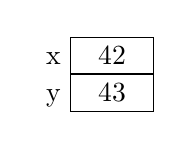
\begin{tikzpicture}[]
\matrix [matrix of nodes, row sep=0, column 2/.style={nodes={rectangle,draw,minimum width=3em}}]
{
x   & 42 \\
y   & 43 \\
};
\end{tikzpicture}
%\end{column}

%\end{columns}

\end{multicols}


\item Med en \Emph{tilldelningssats} ges en tidigare \code{var}-deklarerad variabel ett nytt värde:
\begin{lstlisting}
x = 13
\end{lstlisting}

\item Det gamla värdet försvinner för alltid och det nya värdet lagras istället: \\
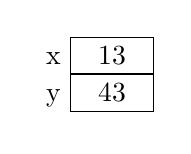
\begin{tikzpicture}[]
\matrix [matrix of nodes, row sep=0, column 2/.style={nodes={rectangle,draw,minimum width=3em}}]
{
x   & 13 \\
y   & 43 \\
};
\end{tikzpicture}

Observera att \code{y} här inte påverkas av att x ändrade värde.
\end{itemize}
\end{Slide}

\begin{Slide}{Tilldelningssatser är \emph{inte} matematisk likhet}\SlideFontSmall

\begin{itemize}

\item Likhetstecknet används alltså för att \Emph{tilldela} variabler nya värden och det är \Alert{inte} samma sak som matematisk likhet. Vad händer här?
\begin{lstlisting}
x = x + 1
\end{lstlisting}

\item Denna syntax är ett arv från de gamla språken C, Fortran mfl.

\item I \href{https://en.wikipedia.org/wiki/Assignment_(computer_science)}{andra språk} används  t.ex.  \\\vspace{1em}
\texttt{x := x + 1}  \hspace{2em} eller  \hspace{2em} \texttt{x <- x + 1} \\\vspace{0.5em}

\item Denna syntax visar kanske bättre att tilldelning är en \Emph{stegvis process}:

\begin{enumerate}\SlideFontTiny
\item Först beräknas \Emph{uttrycket till höger} om tilldelningstecknet.
\item Sedan \Emph{ersätts värdet} som variabelnamnet refererar till av det beräknade uttrycket. Det gamla värdet \Alert{försvinner för alltid}.
\end{enumerate}

\end{itemize}

\end{Slide}


\begin{Slide}{Förkortade tilldelningssatser}
\begin{itemize}
\item Det är vanligt att man vill tilldela en variabel ett nytt värde som beror av det gamla, så som i \\\code{x = x + 1}

\item Därför finns \Emph{förkortade tilldelningssatser} som gör så att man sparar några tecken och det blir tydligare (?) vad som sker (när man vant sig vid detta skrivsätt):
\begin{Code}
x += 1
\end{Code}

\item Uttrycket ovan expanderas av kompilatorn till \code{x = x + 1}
\end{itemize}


\end{Slide}


\begin{Slide}{Exempel på förkortade tilldelningssatser}
\begin{REPLnonum}
scala> var x = 42
val x: Int = 42

scala> x *= 2

scala> x
val res0: Int = 84


scala> x /= 3

scala> x
val res1: Int = 28
\end{REPLnonum}
\end{Slide}


\ifkompendium\else
\begin{Slide}{Övning: Tilldelningar i sekvens}\footnotesize

%\begin{columns}
%\begin{column}{0.32\textwidth}
\begin{minipage}{0.32\textwidth}

Rita hur minnet ser ut efter varje rad nedan:
\vskip1em
\begin{lstlisting}[ numbers=left,]
var u = 42
var x = 10
var y = 2 * x + 1
x = 20
var z = y + x + y - x
x += 1; y *= 2
\end{lstlisting}
%\end{column}
\end{minipage}\hspace{2em}%
%\begin{column}{0.6\textwidth}
\begin{minipage}{0.6\textwidth}


\scriptsize En variabel som ännu inte \Emph{initierats} har ett \Alert{odefinierat} värde, anges nedan med frågetecken.
\begin{table}[]
\centering\scriptsize
%http://tex.stackexchange.com/questions/83930/what-are-the-different-kinds-of-boxes-in-latex
\newcommand{\mybox}[1]{\raisebox{-0.5mm}{\framebox(21,14){#1}}\vspace{0.5mm}}
\begin{tabular}{@{}ccccccc}
 & rad 1 & rad 2 & rad 3 & rad 4  & rad 5 & rad 6\\
u& \mybox{42 } &  \mybox{}   &   \mybox{}   & \mybox{} & \mybox{} & \mybox{} \\
x& \mybox{? } &  \mybox{}   &   \mybox{}   & \mybox{} & \mybox{}  & \mybox{} \\
y& \mybox{? } &  \mybox{}   &   \mybox{}   & \mybox{} & \mybox{}  & \mybox{} \\
z& \mybox{? } &  \mybox{}   &   \mybox{}   & \mybox{} & \mybox{}  & \mybox{} \\
\end{tabular}
\end{table}

%\end{column}
%\end{columns}
\end{minipage}%
\end{Slide}
\fi



\begin{Slide}{Variabler som ändrar värden kan vara knepiga}
\begin{itemize}
\item Kod som innehåller variabler som \Alert{förändras} över tid är ofta svårare att läsa och begripa.

\item Många buggar beror på att variabler av misstag förändras på felaktiga och oanade sätt.

\item Föränderliga värden blir speciellt svåra i kod som körs jämlöpande (parallellt).

\item I kod som körs i skarpt läge med många användare (s.k. produktionskod) är därför \code{val} att föredra, medan \code{var} endast används om det \Alert{verkligen} behövs.
\item Alltså: räkna hellre ut nya värden än förändra befintliga.
\end{itemize}
\end{Slide}
%%%%%%%%%%


\Subsection{Kontrollstrukturer}

\begin{Slide}{Kontrollstrukturer: alternativ och repetition}\SlideFontSmall
Används för att kontrollera (förändra) sekvensen och skapa \Emph{alternativa} vägar genom koden. Vägen  bestäms vid körtid.
\begin{itemize}
\item if-sats:
\begin{Code}
if math.random() < 0.8 then println("gurka") else println("tomat")
\end{Code}
\end{itemize}

Olika sorters \Emph{loopar} för att repetera satser. Antalet repetitioner ges vid körtid.
\begin{itemize}
\item \code{while}-sats: bra när man \Alert{inte vet hur många gånger} det kan bli.
\begin{Code}
while math.random() < 0.8 do println("gurka")
\end{Code}

\item \code{for}-sats: bra när man \Alert{vill ange antalet repetitioner}:
\begin{Code}
for i <- 1 to 10 do println(s"gurka nr $i")
\end{Code}

\end{itemize}
\end{Slide}

\begin{Slide}{Scala-2-syntax för kontrollstrukturer fungerar i Scala 3}\SlideFontSmall
I Scala 2 användes en gammal syntax för kontrollstrukturer som liknar mer C/C++/Java. Den är tillåten i Scala 3, men nya mer lättlästa syntaxen är att föredra.
\begin{itemize}
\item Scala-2-syntax för alternativ: parenteser men inget \code{then}
\begin{Code}
if (math.random() < 0.8) println("gurka") else println("tomat")
\end{Code}
\end{itemize}

Scala-2-syntax för repetition:
\begin{itemize}
\item \code{while}-sats: parenteser men inget \code{do}
\begin{Code}
while (math.random() < 0.8) println("gurka")
\end{Code}

\item \code{for}-sats: parenteser men inget \code{do}
\begin{Code}
for (i <- 1 to 10) println(s"gurka nr $i")
\end{Code}

\item Kojo Desktop funkar ännu bara med Scala 2 och gamla syntaxen, men Kojo kan även köras med Scala 3 (se hur i kompendiet).

\end{itemize}

\end{Slide}

\begin{Slide}{Repetera många satser}
Om du vill göra flera saker i sekvens inne i en repetition så kan du skriva flera satser inom \Emph{klammer-parenteser}:
\begin{Code}
while math.random() < 0.8 do {
  println("gurka")
  println("tomat")
}
println("Repetitionen är klar!")
\end{Code}
\pause
Du kan efter vissa nyckelord (t.ex. \code{do}, \code{then}, \code{else}) välja bort klammer-parenteser \Eng{optional braces}. 
\begin{Code}
while math.random() < 0.8 do
  println("gurka")
  println("tomat")

println("Repetitionen är klar!")
\end{Code}
Då är det \Emph{indenteringen} som avgör vilka satser som ingår. \\Detta fungerar i Scala 3 (men inte i Scala 2).
\end{Slide}


\begin{Slide}{Procedurer}\SlideFontSmall
\begin{itemize}
\item En \Emph{procedur} är en funktion som \Alert{gör} något intressant, men som \Alert{inte} lämnar något intressant returvärde.
\item Exempel på procedur i standardbiblioteket: \code{println("hej")}
\item Du \Emph{deklarerar egna procedurer} genom att ange \texttt{\Alert{Unit}} som returvärdestyp. Då returneras värdet \texttt{\Alert{()}} som betyder ''inget''.
\end{itemize}
\begin{REPLnonum}
scala> def hej(x: String): Unit = println(s"Hej på dej $x!")
hej: (x: String)Unit

scala> hej("Herr Gurka")
Hej på dej Herr Gurka!

scala> val x = hej("Fru Tomat")
Hej på dej Fru Tomat!
x: Unit = ()
\end{REPLnonum}
\begin{itemize}
\item Det som \Alert{görs} kallas (sido)\Emph{effekt}. Ovan är utskriften själva effekten.
\item Även funktioner kan ha sidoeffekter. De kallas då \Alert{oäkta} funktioner.
\end{itemize}
\end{Slide}

\begin{Slide}{Problemlösning: nedbrytning i abstraktioner som sen kombineras}\SlideFontSmall
\begin{itemize}
\item En av de allra viktigaste principerna inom programmering är \Emph{funktionell nedbrytning} där  \Emph{underprogram} i form av funktioner och procedurer skapas för att bli byggstenar som kombineras till mer avancerade funktioner och procedurer.

\item Genom de namn som definieras skapas \Emph{återanvändbara abstraktioner} som kapslar in det funktionen gör till ett ''byggblock''.

\item Bra ''byggblock'' gör det lättare att lösa svåra programmeringsproblem.

\item Abstraktioner som beräknar eller gör \Emph{en enda, väldefinierad sak} är enklare att använda, jämfört med de som gör många, helt olika saker.

\item Abstraktioner med \Emph{välgenomtänkta namn} är enklare att använda, jämfört med kryptiska eller missvisande namn.
\end{itemize}

\end{Slide}

\Subsection{Veckans uppgifter}

\begin{Slide}{Övning \texttt{expressions} och labb \texttt{kojo}}
\label{w01:kojo-slide}
\begin{itemize}
  \item På övningen kör du Scala REPL för att träna på SARA.
  \item[] \Alert{Läs i Appendix} och på kursens hemsida under ''Verktyg'' om hur du installerar och får igång Scala REPL.
  \item På laborationen använder du barnvänliga \Emph{Kojo} för träna på SARA, med fokus på abstraktion.
  \item Det finns tre olika sätt att använda Kojo:
  \begin{enumerate}
  \item Grafikbiblioteket \textbf{\texttt{kojolib}} i ett fristående Scala program med hjälp av en professionell kodeditor och kompilering och exekvering i terminalen. \Emph{Fungerar fint med nya Scala 3}.
  \item Skrivbordsappen \textbf{Kojo Desktop} med inbyggd barnvänlig editor (endast Scala 2).
  \item Webbappen \textbf{\url{http://kojo.lu.se/}} som körs direkt i din webbläsare (endast Scala 2, begränsade funktioner).
  \end{enumerate}
\end{itemize}  
Alternativ 1 rekommenderas, men om du försenas av tekniskt strul, så kom igång med 2 el. 3 så länge tills du fått hjälp.
\end{Slide}

\ifkompendium\else

\begin{SlideExtra}{Om veckans övning: \code{expressions}}\SlideFontSmall

\begin{itemize}
%!TEX encoding = UTF-8 Unicode

\item Förstå vad som händer när satser exekveras och uttryck evalueras.
\item Förstå sekvens, alternativ och repetition.
\item Känna till litteralerna för enkla värden, deras typer och omfång.
\item Kunna deklarera och använda variabler och tilldelning, samt kunna rita bilder av minnessituationen då variablers värden förändras.
\item Förstå skillnaden mellan olika numeriska typer, kunna omvandla mellan dessa och vara medveten om noggrannhetsproblem som kan uppstå.
\item Förstå booleska uttryck och värdena \code{true} och \code{false}, samt kunna förenkla booleska uttryck.
\item Förstå skillnaden mellan heltalsdivision och flyttalsdivision, samt användning av rest vid heltalsdivision.
\item Förstå precedensregler och användning av parenteser i uttryck.
\item Kunna använda \code{if}-satser och \code{if}-uttryck.
\item Kunna använda \code{for}-satser och \code{while}-satser.
\item Kunna använda \code{math.random()} för att generera slumptal i olika intervaller.
\item Kunna beskriva skillnader och likheter mellan en procedur och en funktion.

\end{itemize}

\end{SlideExtra}

\begin{SlideExtra}{Om veckans labb: \code{kojo}}
\begin{itemize}
%!TEX encoding = UTF-8 Unicode
%!TEX root = ../compendium2.tex

\item Kunna tillämpa och kombinera principerna sekvens, alternativ, repetition, och abstraktion i skapandet av egna program om minst 20 rader kod.
\item Kunna förklara vad ett program gör i termer av sekvens, alternativ, repetition, och abstraktion.
\item Kunna formatera egna program så att de blir lätta att läsa och förstå.
\item Kunna förklara vad en variabel är och kunna deklarera oföränderliga och förändringsbara variabler, samt göra tilldelningar.
\item Kunna genomföra upprepade varv i cykeln \emph{editera-exekvera-felsöka/förbättra} för att stegvis bygga upp allt mer utvecklade program.

\end{itemize}
\end{SlideExtra}

\fi

%%%%%%%%%%%%%%%%%%%%%%%%%%%%%%%%%%%%%% nedan redan meddelat i introveckan
%\ifkompendium\else
%\Subsection{Meddelande från \href{http://lth.se/code}{Code@LTH}}
%\fi









%!TEX encoding = UTF-8 Unicode
%!TEX root = ../compendium1.tex

\renewcommand{\vecka}{2}

\chapter{Kodstrukturer}
\begin{itemize}[nosep]
\item while-sats
\item for-sats
\item algoritm: min/max
\item MIN_VALUE
\item MAX_VALUE
\item paket
\item import
\item filstruktur
\item jar
\item dokumentation
\item programlayout
\item JDK
\item konstanter vs föränderlighet
\item objektorientering
\item klasser
\item objekt
\item referensvariabler
\item referenstilldelning
\item anropa metoder
\item SimpleWindow\end{itemize}
\clearpage\section{Teori}
%!TEX encoding = UTF-8 Unicode
%!TEX root = ../lect-w02.tex


\ifkompendium

\noindent Ett program innehåller satser och uttryck. En \Emph{kontrollstruktur}, t.ex. \code{while}, styr i vilken \Alert{ordning} satser och uttryck exekveras. Data kan placeras i en \Emph{datastruktur}, t.ex. en \code{Vector}, så att man senare kan komma åt data igen.    
\fi


\ifkompendium\else
\begin{SlideExtra}{Från förra veckan: \texttt{val} \texttt{var} \texttt{def}}
  Vad är det för skillnad på (och likhet mellan) \code{val}, \code{var} och \code{def}? \pause
  \begin{itemize}
    \item Med \code{val} deklareras en variabel som tilldelas ett värde vid initialisering och som sedan \Emph{aldrig ändras}.
    \item Med \code{var} deklareras en variabel som tilldelas ett värde vid initialisering och som sedan \Alert{kan uppdateras} hur många gånger som helst med hjälp av tilldelningssatser.
    \item Med \code{def} deklareras en funktion som körs vid \Emph{varje anrop}
  \end{itemize}
  \pause\vspace{1em} En \Alert{konstighet i REPL}: 
  \begin{itemize}
  \item Man kan i REPL \Emph{deklarera} variabler och funktioner med \Emph{samma namn} \Alert{flera gånger} på samma nivå. 
  \item Detta ger i vanliga, fristående program \Emph{kompileringsfel}. 
  \end{itemize}
\end{SlideExtra}

\begin{SlideExtra}{Från förra veckan: \texttt{if} \texttt{then} \texttt{else}}\SlideFontSmall
\Emph{Spelets regler:} Singla slant. Om du får krona har du vunnit. \\[0.5em]
Förenkla dessa if-uttryck:
\begin{Code}
def singlaSlant: Boolean = if math.random() < 0.5 then true else false

def harVunnit(slantÄrKrona: Boolean): Boolean = 
  if slantÄrKrona == true then true else false
\end{Code}
\pause förenkling av ''kaka-på-kaka'': \textbf{if uttryck then true else false}
\begin{Code}
def singlaSlant: Boolean = math.random() < 0.5
\end{Code}
\pause förenkling av ''kaka-på-kaka'':  \textbf{uttryck == true}
\begin{Code}
def harVunnit(slantÄrKrona: Boolean): Boolean = slantÄrKrona
\end{Code}
\pause Hur ska vi ändra \code{harVunnit} om vi ändrar reglerna till att Klave ger vinst? \\
\pause Repetera även \Alert{de Morgans lagar} från vecka 1 så du har koll på dem.
\end{SlideExtra}

\fi 

\Subsection{Datastrukturer}

\begin{Slide}{Vad är en datastruktur?}\SlideFontSmall
\begin{itemize}
\item En \href{https://sv.wikipedia.org/wiki/Datastruktur}{datastruktur} är en struktur för organisering av data som...
\begin{itemize}\SlideFontTiny
\item kan innehålla \Alert{många} element,
\item kan \Emph{refereras} till som en \Alert{helhet}, och
\item ger möjlighet att \Emph{komma åt} \Alert{enskilda element}.
\end{itemize}

\item En \Emph{samling} \Eng{collection} är en datastruktur som kan innehålla många element av \Alert{samma typ}.

\item Exempel på olika samlingar där elementen är organiserade på olika vis: \\
\vspace{0.5em}
\begin{tabular}{l c}
\Emph{Sekvens} & \includegraphics[width=5cm]{../img/list.pdf} \\
\Emph{Träd}  & \includegraphics[width=2.2cm]{../img/tree.pdf} \\
\Emph{Graf}  & \includegraphics[width=2.2cm]{../img/graph.pdf} \\
\end{tabular}
\end{itemize}
{
\SlideFontTiny \vspace{1em }\hskip2em
Mer om sekvenser \& träd i \href{https://cs.lth.se/edaa01vt}{EDAA01 pfk}.
Mer om träd, grafer i \href{https://cs.lth.se/edaa40}{Diskreta strukturer.}
}

\end{Slide}

\begin{Slide}{Några samlingar i \texttt{scala.collection}}\SlideFontSmall
\SlideOnly{\setlength{\leftmargini}{0pt}}
\begin{itemize}
\item En \Emph{samling} \Eng{collection} är en datastruktur som kan innehålla många element av \Alert{samma typ}.
\item En \Emph{sekvens} \Eng{sequence} är en samling där alla element är ordnade.

\item Exempel på \Emph{färdiga samlingar} i Scalas standardbibliotek där elementen är organiserade  internt på \Alert{olika} vis så att samlingen får olika egenskaper som passar \Alert{olika användningsområden}:
\begin{itemize}\SlideFontTiny
\item \texttt{scala.collection.immutable.\Emph{Vector}}, sekvens med snabb access \Alert{överallt}.
\item \texttt{scala.collection.immutable.\Emph{List}}, sekvens med snabb access \Alert{i början}.
\item \texttt{scala.collection.immutable.\Emph{Set}}, \texttt{scala.collection.\Alert{mutable}.\Emph{Set}}, mängd med unika element; ej i sekvens men snabb innehållstest.
\item \texttt{scala.collection.immutable.\Emph{Map}}, \texttt{scala.collection.\Alert{mutable}.\Emph{Map}}, mängd med par av nyckel \& tillhörande värde, snabb access via nyckel.
\item \texttt{scala.collection.\Alert{mutable}.\Emph{ArrayBuffer}}, förändringsbar sekvens kan ändra storlek.
\item \texttt{scala.\Emph{Array}}, förändringsbar sekvens som \Alert{inte} kan ändra storlek. Alla element är lagrade efter varandra i minnet: snabbast access av alla samlingar, men har speciella begränsningar.
\end{itemize}
\end{itemize}
\end{Slide}


\begin{Slide}{Olika strukturer för att hantera data}
\begin{itemize}\SlideFontSmall
\item \Emph{Tupel} \Eng{tuple}
\begin{itemize}\SlideFontTiny
\item samla flera datavärden t.ex. \code{(1, "hej", true)} i element \Emph{\code{_1}}, \Emph{\code{_2}}, \Emph{\code{_3}} 
\item elementen kan vara av \Alert{olika} typ
\end{itemize}
\item \Emph{Enumeration} (även kallad \emph{uppräkning}) \Eng{enumeration}
\begin{itemize}\SlideFontTiny
\item Namnge uppräknade värden t.ex. \code+enum Color { case Red, Black }+
\item Värdena har ordningsnummer och är alla av \Alert{samma} typ (här \code{Color})
\end{itemize}
\item \Emph{Klass} \Eng{class}
\begin{itemize}\SlideFontTiny
\item samlar data i \Emph{attribut} med (väl valda!) namn
\item attributen kan vara av \Alert{olika} typ
\item definierar även \Emph{metoder} som använder attributen \\ (kallas även \Emph{operationer} på data)
\end{itemize}

\item \Emph{Färdig samling}
  \begin{itemize}
  \item speciella klasser som samlar data i element av \Alert{samma} typ
  \item exempel: \code{scala.collection.immutable.}\Emph{\code{Vector}}
  \item har ofta \emph{många} färdiga \Emph{bra-att-ha-metoder}, \\ se snabbreferensen \url{https://cs.lth.se/pgk/quickref}
  \end{itemize}

\item \Emph{Egenimplementerade samlingar}
  \begin{itemize}
  \item $\rightarrow$ fördjupningskurs
  \end{itemize}

\end{itemize}
\end{Slide}





\begin{Slide}{Vad är en vektor?}\SlideFontSmall
En \Emph{vektor}\footnote{Vektor kallas ibland på svenska även \href{https://sv.wikipedia.org/wiki/F\%C3\%A4lt_\%28datastruktur\%29}{fält}, men det skapar stor förvirring eftersom det engelska ordet \emph{field} ofta används för \emph{attribut} (förklaras senare).}
\Eng{vector} är en \Emph{sekvens} som är \Alert{snabb} att \Emph{indexera} i.
Åtkomst av element i en sekvens som t.ex. heter \code{xs} sker i Scala med \code{xs.apply(platsnummer)}:

\begin{REPL}
scala> val heltal = Vector(42, 13, -1, 0, 1)
val heltal: scala.collection.immutable.Vector[Int] = Vector(42, 13, -1, 0, 1)

scala> heltal.apply(0)   // platsnummer räknas från noll
val res0: Int = 42

scala> heltal(1)         // man kan i Scala skippa .apply före (
val res1: Int = 13

scala> heltal(5)         // ger körtidsfel då sjätte platsen inte finns
java.lang.IndexOutOfBoundsException: 5
  at scala.collection.immutable.Vector.checkRangeConvert(Vector.scala:132)
\end{REPL}
Utelämnar du \code{.apply} så skapar kompilatorn automatiskt ett anrop av \code{apply}.
\end{Slide}

\begin{Slide}{En konceptuell bild av en vektor}

\begin{REPLnonum}
scala> val heltal = Vector(42, 13, -1, 0, 1)

scala> heltal(0)
val res0: Int = 42
\end{REPLnonum}

\begin{tikzpicture}[font=\ttfamily]
\matrix [matrix of nodes, row sep=0, column 2/.style={nodes={rectangle,draw,minimum width=3em}}] (var) at (0cm, 2.8cm)
{
heltal   &  \makebox(16,12){ }\\
};
\matrix [matrix of nodes, draw=black,row sep=0, column 2/.style={nodes={rectangle,draw,minimum width=4em}}] (vec) at (4cm, 1cm)
{
\textit{plats} &  \\
0   &  \makebox(16,12){42}\\
1   &  \makebox(16,12){13}\\
2   &  \makebox(16,12){-1}\\
3   &  \makebox(16,12){0}\\
4   &  \makebox(16,12){1}\\
};
\filldraw[black] (0.7cm,2.8cm) circle (3pt) node[] (ref) {};
 \draw [arrow] (ref) -- (vec);
\end{tikzpicture}

%\vspace{1em} Elementen ligger på rad någonstans i minnet.
\end{Slide}



\begin{Slide}{En samling strängar}

\begin{itemize}
\item En vektor kan lagra \Emph{många} värden av samma typ.
\item Elementen kan vara till exempel heltal eller strängar.
\item Eller faktiskt vad som helst. (En s.k. \emph{generisk} samling.)
\end{itemize}

\begin{REPL}
scala> val grönsaker = Vector("gurka","tomat","paprika","selleri")
grönsaker: scala.collection.immutable.Vector[String] =
  Vector(gurka, tomat, paprika, selleri)

scala> val g = grönsaker(1)
val g: String = tomat

scala> val xs = Vector(42, "gurka", true, 42.0)
val xs: Vector[Matchable] = Vector(42, gurka, true, 42.0)
\end{REPL}
\SlideFontSmall Notera typen \code{Matchable} som betyder ''\Emph{nästan vilken typ som helst}''\\
%\footnote{
%(\code{Matchable} liknar \code{Object} i Java/C\# men är \Alert{mer generell}; 
(Mer om \code{Matchable} senare.)
%}
\end{Slide}



\Subsection{Kontrollstrukturer}


\begin{Slide}{Vad är en kontrollstruktur?}
\begin{itemize}
\item En \Emph{kontrollstruktur} påverkar i vilken ordning (sekvens) satser exekveras och uttryck evalueras.
\begin{itemize}
\item[] Exempel på \Emph{inbyggda} kontrollstrukturer:
\\\vspace{0.5em}\code{for}-\code{do}-sats \\ \code{while}-\code{do}-sats \\ \code{for}-\code{yield}-uttryck
\end{itemize}

\item[]

\item I Scala kan man definiera \Alert{egna} kontrollstrukturer.
\begin{itemize}
\item[] Exempel: \code{upprepa} som du använt i Kojo
\\\vspace{0.5em}\code|upprepa(4){fram; höger}|
\end{itemize}
\end{itemize}
\end{Slide}

\ifkompendium\else
\begin{SlideExtra}{Mitt första program: en oändlig loop på ABC80}
\begin{minipage}{0.8\textwidth}
\begin{verbatim}
10 print "hej"
20 goto 10
\end{verbatim}
\includegraphics[width=0.8\textwidth]{../img/abc80.jpg}
\end{minipage}%
\begin{minipage}{0.2\textwidth}
\pause
\begin{verbatim}
hej
hej
hej
hej
hej
hej
hej
hej
hej
hej
hej
hej
<Ctrl+C>
\end{verbatim}
\end{minipage}
\end{SlideExtra}
\fi

\begin{Slide}{Loopa genom elementen i en vektor}
En \code{for}-\code{do}-\Emph{sats} som skriver ut alla element i en vektor:
\begin{REPL}
scala> val grönsaker = Vector("gurka","tomat","paprika","selleri")

scala> for g <- grönsaker do println(g)
gurka
tomat
paprika
selleri

\end{REPL}
\code{for ... do ...} gör så att följande händer:
\begin{itemize}
  \item Plocka ut \Emph{varje element} ur samlingen. 
  \item \Emph{Namnet} före pilen (här \code{g}) \Alert{refererar} till ett \Emph{nytt} värde för varje runda i loopen.
  \item Detta namn motsvarar en \Emph{lokal} \code{val}-variabel.
\end{itemize}
\end{Slide}


\begin{Slide}{Bygg ny samling från befintlig med for-yield-uttryck}
Ett \code{for}-\code{yield}-\Emph{uttryck} som \Emph{skapar en \Alert{ny} samling}.

\begin{Code}[basicstyle=\ttfamily\fontsize{12}{14}\selectfont]
for g <- grönsaker yield s"god $g"
\end{Code}

\begin{REPL}
scala> val grönsaker = Vector("gurka","tomat","paprika","selleri")

scala> val åsikter = for g <- grönsaker yield s"god $g"
val åsikter: Vector[String] =
  Vector(god gurka, god tomat, god paprika, god selleri)
\end{REPL}

\end{Slide}


\begin{Slide}{Samlingen \code{Range} håller reda på intervall}
\begin{itemize}
\item Med en \code{Range(start, slut)} kan du skapa ett \Emph{intervall}: \\ från och med \code{start} till (men inte med) \code{slut}
\end{itemize}

\begin{REPLnonum}
scala> Range(0, 42)
val res0: Range =
  Range(0, 1, 2, 3, 4, 5, 6, 7, 8, 9, 10, 11, 12, 13, 14,
    15, 16, 17, 18, 19, 20, 21, 22, 23, 24, 25, 26, 27, 28,
    29, 30, 31, 32, 33, 34, 35, 36, 37, 38, 39, 40, 41)
\end{REPLnonum}

\begin{itemize}
\item Men alla värden däremellan skapas inte förrän de behövs:
\end{itemize}

\begin{REPL}
scala> val jättestortIntervall = Range(0, Int.MaxValue)
val jättestortIntervall: Range.Exclusive = Range 0 until 2147483647

scala> jättestortIntervall.end
val res1: Int = 2147483647

scala> jättestortIntervall.toVector
java.lang.OutOfMemoryError: Java heap space
\end{REPL}

\end{Slide}

\begin{Slide}{Loopa med Range}
\code{Range} används i for-loopar för att hålla reda på antalet rundor.
\begin{REPLsmall}
scala> for i <- Range(0, 6) do print(s" gurka $i")
 gurka 0 gurka 1 gurka 2 gurka 3 gurka 4 gurka 5
\end{REPLsmall}
Du kan skapa en \code{Range} med \code{until} efter ett heltal:
\begin{REPLsmall}
scala> 1 until 7
val res1: Range =
  Range(1, 2, 3, 4, 5, 6)

scala> for i <- 1 until 7 do print(s" tomat $i")
 tomat 1 tomat 2 tomat 3 tomat 4 tomat 5 tomat 6

\end{REPLsmall}
Med metoden \code{indices} på kan du få en \code{Range} med alla index:
\begin{REPLsmall}
scala> val xs = Vector("gurka1","gurka2","tomat1")
val xs: Vector[String] = Vector(gurka1, gurka2, tomat1)

scala> xs.indices
val res0: Range = Range 0 until 3
\end{REPLsmall}
\end{Slide}

\begin{Slide}{Loopa med Range skapad med \texttt{to}}

Med \code{to} efter ett heltal får du en \code{Range} till och \Emph{med} sista:
\begin{REPLnonum}
scala> 1 to 6
res2: Range.Inclusive =
  Range(1, 2, 3, 4, 5, 6)

scala> for i <- 1 to 6 do print(" gurka " + i)
 gurka 1 gurka 2 gurka 3 gurka 4 gurka 5 gurka 6

\end{REPLnonum}


\end{Slide}



\begin{Slide}{Vad är en \code{Array}?}


\begin{itemize}
\item En \href{https://en.wikipedia.org/wiki/Array_data_structure}{\code{Array}} liknar en \code{Vector} men har en särställning i JVM:
\begin{itemize}
\item Lagras som en sekvens i minnet på efterföljande adresser.
\item \Emph{Fördel}: snabbaste samlingen för element-access i JVM.
\item Men det finns en hel del \Alert{nackdelar} som vi ska se senare.
\end{itemize}

\end{itemize}

\begin{REPLnonum}
scala> val heltal = Array(42, 13, -1, 0 , 1)
\end{REPLnonum}

\begin{tikzpicture}[font=\ttfamily,scale=0.75, every node/.style={scale=0.75}]
\matrix [matrix of nodes, row sep=0, column 2/.style={nodes={rectangle,draw,minimum width=3em}}] (var) at (0cm, 2.8cm)
{
heltal   &  \makebox(16,12){ }\\
};
\matrix [matrix of nodes, draw=black,row sep=0, column 2/.style={nodes={rectangle,draw,minimum width=4em}}] (vec) at (4cm, 1cm)
{
\textit{plats} &  \\
0   &  \makebox(16,12){42}\\
1   &  \makebox(16,12){13}\\
2   &  \makebox(16,12){-1}\\
3   &  \makebox(16,12){0}\\
4   &  \makebox(16,12){1}\\
};
\filldraw[black] (0.7cm,2.8cm) circle (3pt) node[] (ref) {};
 \draw [arrow] (ref) -- (vec);
\end{tikzpicture}
\end{Slide}

\begin{Slide}{Några likheter \& skillnader mellan \texttt{Vector} och \texttt{Array}}\SlideFontSmall
\begin{multicols}{2}
\begin{REPLnonum}
scala> val xs = Vector(1,2,3)
\end{REPLnonum}

\columnbreak

\begin{REPLnonum}
scala> val xs = Array(1,2,3)
\end{REPLnonum}
\end{multicols}


Några likheter mellan \texttt{Vector} och \texttt{Array}
\begin{itemize}
\item Båda är samlingar som kan innehålla många element.

\item Med båda kan man snabbt accessa vilket element som helst: \code{xs(2)}
\end{itemize}
Några viktiga skillnader:

\vspace{-0.5em}\begin{multicols}{2}
\Emph{Vector}
\begin{itemize}
\item Är \Emph{oföränderlig}: du kan lita på att elementreferenserna aldrig någonsin kommer att ändras.

\item Är \Emph{snabb på att skapa en delvis förändrad kopia}, t.ex. tillägg/borttagning/uppdatering mitt i sekvensen.

\end{itemize}


\columnbreak

\Alert{Array}
\begin{itemize}
\item Är \Alert{föränderlig}: \code{xs(2) = 42}

\item Är \Alert{snabb} om man bara vill läsa eller skriva på befintliga platser.

\item Kan \Alert{ej} ändra storlek: tillägg eller borttagning mitt i kräver \Alert{långsam} kopiering av resten.

\end{itemize}
\end{multicols}
\end{Slide}



\Subsection{Fristående applikation}

\begin{Slide}{Kompilering i terminalen}
  När du ska skriva kod i en editor, kompilera i terminalen och köra ditt program som en \Emph{fristående applikation}, så behövs: 
  \begin{itemize}
    \item En editor: \Emph{VS Code} med tillägget \Alert{Scala (Metals)}
    \item Körmiljön \Emph{OpenJDK} 
    \item Kommandoverktyg i terminalen: \Alert{\texttt{scala}} eller \texttt{scala-cli}
    \item Installera så här: \url{https://cs.lth.se/pgk/verktyg}
    \item Läs mer i Appendix C.
    \item Tips om du kör Windows: installera %\href{https://docs.microsoft.com/en-us/windows/terminal/get-started}
    {nya Windows Terminal}

  \end{itemize}
    Få hjälp i kanalerna \texttt{\#installationskrångel} och \texttt{\#frågor-och-svar} på vår Discord-server eller fråga handledare på resurstid.
  
\end{Slide}

\begin{Slide}{Scala Command Line Interface (CLI)}
\begin{itemize}
\item Utvecklingen av ett nytt kommandogränssnitt \Eng{Command Line Interface (CLI)} för Scala startades 2022 i ett öppenkällkodsprojekt som leds av Virtuslab. 
\item I augusti 2024 blev \Alert{\texttt{scala-cli}} det nya \Emph{\texttt{scala}}%\footnote{I skrivande stund så har skiftet ännu inte skett. När det sker kan du ersätta alla förekomster av \code{scala-cli} med det kortare \code{scala}.}
\item Du kan nu ersätta \code{scala-cli} med \code{scala}
\item Läs mer i Appendix C och F, samt här: \url{https://scala-cli.virtuslab.org/}
\item Se vad Scala CLI kan göra med underkommandot \texttt{help}
\begin{REPLnonum}
  scala help
\end{REPLnonum}
\end{itemize}
\end{Slide}

\begin{Slide}{Ett minimalt fristående program i Scala}\SlideFontSmall
Spara nedan Scala-kod i filen \code{hej.scala}:
\begin{Code}
@main def run = println("Hej Scala!")
\end{Code}

Kompilera och kör i terminalen:
\begin{REPL}
> scala run hej.scala 
Compiling project (Scala 3.5.0, JVM (21))
Compiled project (Scala 3.5.0, JVM (21))
Hej Scala! 
\end{REPL}

Innan körning kompileras dina kodfiler automatiskt vid behov. Du kan se maskinkoden i en underkatalog i till katalogen \texttt{.scala-build}: 
\begin{REPL}
> ls .scala-build/*/classes/main
'hej$package.class'  'hej$package$.class'  'hej$package.tasty'   run.class   run.tasty
\end{REPL}
\end{Slide}


\begin{Slide}{Loopa genom en samling med en \texttt{while}-sats}
\begin{REPLnonum}
scala> val xs = Vector("Hej","på","dej","!!!")
val xs: Vector[String] =
  Vector(Hej, på, dej, !!!)

scala> xs.size
val res0: Int = 4

scala> var i = 0
val i: Int = 0

scala> while i < xs.size do { println(xs(i)); i = i + 1 }
Hej
på
dej
!!!
\end{REPLnonum}
\end{Slide}


\begin{Slide}{Strängargument till i ett program med primitiv main}
Skriv och spara nedan kod i filen \texttt{helloargs1scala}
\begin{REPLnonum}
> code helloargs1.scala
\end{REPLnonum}
\begin{Code}
object HelloScalaArgs:
  def main(args: Array[String]): Unit = // en primitiv main-metod utan @main
    var i = 0
    while i < args.size do
      println(args(i))
      i = i + 1
\end{Code}
En primitiv \code{main}-metod har ej \code{@main} och måste vara i ett objekt. \\
Kompilera och kör med programargument efter \code{--}
\begin{REPL}
> scala run helloargs1.scala -- morot gurka tomat
morot
gurka
tomat
\end{REPL}
\end{Slide}

\begin{Slide}{Typsäkra argument till i ett program med @main}
  \SlideFontSmall
Skriv och spara nedan kod i filen \texttt{helloargs2.scala}
\begin{REPLnonum}
> code helloargs2.scala
\end{REPLnonum}
\begin{Code}
@main def hej(heltal: Int, resten: String*): Unit =  // notera * efter String
  for i <- 0 until heltal do println(resten(i))
\end{Code}
Med \code{@main} behövs inget objekt.\\
Kompilera och kör med programargument efter \code{--}
\begin{REPL}
> scala run helloargs2.scala -- 2 morot gurka tomat
morot
gurka
> scala run helloargs2.scala -- aj morot gurka tomat
Illegal command line: java.lang.NumberFormatException: For input string: "aj"
\end{REPL}
Med \code{@main} genereras automatiskt en primitiv main som kollar att argumenten har rätt typ.
\end{Slide}


\begin{Slide}{För kännedom: Scala-\textbf{skript}}
\begin{itemize}
  \SlideFontSmall
  \item 
Scala-kod kan köras som ett \Emph{skript}.
\item Ett skript finns i en enda fristående fil med ändelsen \code{.sc}
\item Skript behöver inget huvudprogram. 
\item Skript har automatiskt alla programargument i strängsekvensen \code{args}

\begin{Code}
// spara detta i filen 'myscript.sc'
println("Hej alla mina argument:")
for a <- args do println(s"Hej: $a") 
\end{Code}
\begin{REPLnonum}
> scala run myscript.sc -- ett två tre
Hej alla mina argument:
Hej: ett
Hej: två
Hej: tre
\end{REPLnonum}
\end{itemize}
\pause {\SlideFontTiny Ett Scala-skript kan ej anropa andra skript utan speciella åtgärder, se detaljer här: \url{https://scala-cli.virtuslab.org/docs/guides/scripting/scripts/}
}
\end{Slide}



\Subsection{Algoritmer: stegvisa lösningar}

\begin{Slide}{Vad är en algoritm?}
En \href{https://sv.wikipedia.org/wiki/Algoritm}{algoritm} är en sekvens av instruktioner som beskriver hur man löser ett problem.

\vspace{1em}\Emph{Exempel}:
\begin{itemize}
\item	 baka en kaka
\pause\item räkna ut din pensionsprognos
\pause\item köra bil
\pause\item kolla om highscore i ett spel
\end{itemize}
\ifkompendium\else
\begin{tikzpicture}[overlay]
\node[xshift=0.85\textwidth, scale=2.0] { \includegraphics[width=0.25\textwidth]{../img/highscore}};
\end{tikzpicture}
\fi
\end{Slide}


\ifkompendium\else
\begin{SlideExtra}{Algoritm-exempel: HIGHSCORE}
\Emph{Problem}: Kolla om high-score i ett spel \\ \vspace{1em}

\Emph{Varför?} \pause Så att de som spelar uppmuntras att spela mer :) \\ \vspace{1em}

\Emph{Algoritm:}\pause
\begin{enumerate}
\item $points$ $\leftarrow$ poängen efter senaste spelet
\item $highscore$ $\leftarrow$ bästa resultatet innan senaste spelet
\item \Key{om} $points$ är större än $highscore$ \Key{så}
\begin{enumerate}[ ~~]
\item  Skriv ''Försök igen!''
\end{enumerate}
\Key{annars}
\begin{enumerate}[ ~~]
\item  Skriv ''Grattis!''
\end{enumerate}
\end{enumerate}
\pause
\scriptsize \Alert{Hittar du buggen?}

\pause Utskriften blir fel; vänd villkor eller byt plats på grenarna i if-satsen
\end{SlideExtra}
\fi

\ifkompendium\else
\begin{SlideExtra}{HIGHSCORE implementerad i Scala}
\begin{Code}
import scala.io.StdIn.readLine

@main 
def run = 
  val points = readLine("Hur många poäng fick du?").toInt
  val highscore = readLine("Vad var highscore före senaste spelet?").toInt
  val msg = if points > highscore then "GRATTIS!" else "Försök igen!"
  println(msg)
\end{Code}
\SlideFontSmall %(Mer om \code{import} senare.)\\
\pause
Är det en bugg eller en feature att det står\\ \texttt{points > highscore} \\ och inte \\ \texttt{points >= highscore} \\ ?
\pause Man får ej GRATTIS om poäng == highscore vilket är tråkigt :)
\end{SlideExtra}



\fi

\begin{Slide}{Algoritmexempel: N-FAKULTET}
\begin{algorithm}[H]
 \SetKwInOut{Input}{Indata}\SetKwInOut{Output}{Utdata}

 \Input{heltalet $n$}
 \Output{produkten av de första $n$ positiva heltalen}
 ~\\
 $prod \leftarrow 1$ \\
 $i \leftarrow 2$  \\
 \While{$i \leq n$}{
  $prod \leftarrow prod * i$\\
  $i \leftarrow i + 1$
 }
 $prod$
\end{algorithm}
\pause\vspace{1em}
\begin{itemize}\SlideFontSmall
\item Vad händer om $n$ är noll?
\item Vad händer om $n$ är ett?
\item Vad händer om $n$ är två?
\item Vad händer om $n$ är tre?
\end{itemize}
\end{Slide}

\begin{Slide}{Algoritmexempel: MIN}
\begin{algorithm}[H]
 \SetKwInOut{Input}{Indata}\SetKwInOut{Output}{Utdata}

 \Input{Array $args$ med strängar som alla innehåller heltal}
 \Output{minsta heltalet }
 ~\\
 $min \leftarrow$ det största heltalet som kan uppkomma  \\
 $n \leftarrow $ antalet heltal \\
 $i \leftarrow 0$ \\
 \While{$i < n$}{
   $x \leftarrow args(i).toInt$ \\
   \If{( x < $min$)}{$min \leftarrow x$}
   $i \leftarrow i + 1$
 }
 $min$
\end{algorithm}
\pause{\hfill \SlideFontTiny \Emph{Testa med indata}: \code{args = Array("2", "42", "1", "2")}}
\end{Slide}


\Subsection{Funktioner skapar struktur}

\ifkompendium
\noindent En program delas ofta upp i många olika \Emph{funktioner}. En funktion kan ha parametrar och ge ett returvärde. Om du delar upp ditt program i många enkla funktioner med bra namn, så blir ditt program lättare att läsa och begripa. Om en vältestad och buggfri funktion användas på flera ställen, så kan risken för buggar minskas.
\fi 

\begin{Slide}{Mall för funktionsdefinitioner}
\code{def} funktionsnamn(parameterdeklarationer): returtyp = uttryck

\pause\vspace{0.3em}\SlideFontSmall
\Emph{Exempel}:

\begin{Code}[basicstyle=\ttfamily\fontsize{9}{11}\selectfont]
def öka(i: Int): Int = i + 1
\end{Code}
\pause Returtypen kan härledas av kompilatorn:
\begin{Code}[basicstyle=\ttfamily\fontsize{9}{11}\selectfont]
def öka(i: Int) = i + 1
\end{Code}
Men för att få hjälp av kompilatorn är det bra att ange returtyp!

\pause 

Om flera parametrar använd kommatecken. Om flera satser använd indentering (och eventuell valfria klammerparenteser).
\begin{Code}[basicstyle=\ttfamily\fontsize{8}{10}\selectfont]
def isHighscore(points: Int, high: Int): Boolean = {
  val highscore: Boolean = points > high
  if highscore then println(":)") else println(":(")
  highscore
}
\end{Code}
\pause Ovan funktion har \Alert{sidoeffekten} att skriva ut en smiley.
\end{Slide}

\begin{Slide}{Bättre många små abstraktioner som gör en sak var}

\begin{Code}[basicstyle=\ttfamily\fontsize{8}{11}\selectfont]
def isHighscore(points: Int, high: Int): Boolean = points > high

def printSmiley(isHappy: Boolean): Unit =
  if isHappy then println(":)") else print(":(")
\end{Code}

\pause\vspace{1em}
\begin{REPLnonum}
  printSmiley(isHighscore(113,99))
\end{REPLnonum}

\pause
\begin{itemize}
  \item Denna bättre \code{isHighscore} är nu en \Emph{äkta funktion} som alltid ger samma svar för samma inparametrar och \Alert{saknar sidoeffekter}; dessa funktioner är ofta lättare att förstå.
  \item Funktioner som ger ett booleskt värde kallas för \Emph{predikat}.
\end{itemize}

\end{Slide}



\begin{Slide}{Vad är ett block?}

\begin{itemize}
\item Ett block \Emph{kapslar in} flera satser/uttryck och ser ''utifrån'' ut som en enda sats/uttryck.

\item Ett block skapas med hjälp av klammerparenteser (''krullparenteser'')

\item [] {\fontsize{14}{18}\selectfont \code|{ uttryck1; uttryck2; ... uttryckN }|}\\~

\pause

\item I Scala (till skillnad från många andra språk) har ett block ett \Emph{värde} och är alltså ett \Emph{uttryck}.

\item Värdet ges av \Emph{sista uttrycket} i blocket.

\begin{REPLnonum}
scala> val x = { println(1 + 1); println(2 + 2); 3 + 3 }
2
4
x: Int = 6
\end{REPLnonum}


\end{itemize}

\end{Slide}

\begin{Slide}{Namn i block blir \textbf{lokala}}
Synlighetsregler:
\begin{enumerate}
\item Identifierare deklarerade inuti ett block blir \Emph{lokala}.

\item Lokala namn \Alert{överskuggar} namn i yttre block om samma.


\item Namn syns i nästlade underblock.

\end{enumerate}

\begin{REPL}
scala> def a = { val lokaltNamn = 42; println(lokaltNamn) }
scala> a 
42

scala> println(lokaltNamn)                                                                                                                  
1 |println(lokaltNamn)
  |        ^^^^^^^^^^
  |        Not found: lokaltNamn

scala> def b = { val x = 42; { val x = 76; println(x) }; println(x) }
scala> def c = { val x = 42; { val b = x + 1; println(b) } }
scala> b  // vad händer?
scala> c  // vad händer?
\end{REPL}

\end{Slide}


\begin{Slide}{Parameter och argument}

Skilj på parameter och argument!
\begin{itemize}
\item En \Alert{parameter} är det deklarerade namnet som används \Alert{lokalt} i en funktion för att referera till...

\item \Emph{argumentet} som är värdet som skickas med \Emph{vid anrop} och binds till det lokala parameternamnet.

\end{itemize}


\begin{REPLnonum}
scala> val ettArgument = 42

scala> def öka(minParameter: Int) = minParameter + 1

scala> öka(ettArgument)
\end{REPLnonum}


Speciell syntax: anrop med s.k. \Emph{namngivet argument}
\begin{REPLnonum}
scala> öka(minParameter = ettArgument)
\end{REPLnonum}
{\SlideFontSmall Namngivna argument kan ges i valfri ordning; då riskerar man inte fel ordning.}

\end{Slide}

\begin{Slide}{Procedurer}\SlideFontSmall
\begin{itemize}
\item En \Emph{procedur} är en funktion som \Alert{gör} något intressant, men som \Alert{inte} lämnar något intressant returvärde.
\item Exempel på befintlig procedur: \code{println("hej")}
\item Du \Emph{deklarerar egna procedurer} genom att ange \texttt{\Alert{Unit}} som returvärdestyp. Då ges värdet \texttt{\Alert{()}} som betyder ''inget''.
\end{itemize}
\begin{REPLsmall}$%dummydollar 
scala> def hej(x: String): Unit = println(s"Hej på dej $x!")

scala> hej("Herr Gurka")
Hej på dej Herr Gurka!

scala> val x = hej("Fru Tomat")
Hej på dej Fru Tomat!

scala> :type x 
Unit

scala> println(x)    // vad händer?
\end{REPLsmall}
\begin{itemize}
\item Det som \Alert{görs} kallas (sido)\Emph{effekt}. Ovan är utskriften själva effekten.
\item Funktioner kan också ha sidoeffekter. De kallas då \Alert{oäkta} funktioner.
\end{itemize}
\end{Slide}

\begin{Slide}{''Ingenting'' \emph{är} faktiskt någonting i Scala}
\begin{itemize}
\item I många språk (Java, C, C++, ...) är funktioner som saknar värden speciella.
 Java m.fl. har speciell syntax för procedurer med nyckelordet \jcode{void}, men \Alert{inte} Scala.

\item I Scala är procedurer inte specialfall; de är vanliga funktioner som returnerar ett värde som \Emph{representerar} ingenting, nämligen () som är av typen Unit.

\item På så sätt blir procedurer inget undantag utan följer vanlig syntax och semantik precis som för alla andra funktioner.

\item Detta är typiskt för Scala: generalisera koncepten och vi slipper besvärliga undantag! \\(Men vi måste förstå generaliseringen...)


\item [] {\SlideFontSmall
\url{https://en.wikipedia.org/wiki/Void_type}
\url{https://en.wikipedia.org/wiki/Unit_type}
}

\end{itemize}

\end{Slide}

\begin{Slide}{Problemlösning: nedbrytning i abstraktioner som sen kombineras}\SlideFontSmall
\begin{itemize}
\item En av de allra viktigaste principerna inom programmering är \Emph{funktionell nedbrytning} där  \Emph{underprogram} i form av funktioner och procedurer skapas för att bli byggstenar som kombineras till mer avancerade funktioner och procedurer.

\item Genom de namn som definieras skapas \Emph{återanvändbara abstraktioner} som kapslar in det funktionen gör.

\item Problemet blir med bra byggblock lättare att lösa.

\item Abstraktioner som beräknar eller gör \Emph{en enda, väldefinierad sak} är enklare att använda, jämfört med de som gör många, helt olika saker.

\item Abstraktioner med \Emph{välgenomtänkta namn} är enklare att använda, jämfört med kryptiska eller missvisande namn.
\end{itemize}

\end{Slide}



\begin{Slide}{Exempel på \textbf{funktionell nedbrytning}}

Kojo-labben gav exempel på \Emph{funktionell nedbrytning} där ett antal abstraktioner skapas och återanvänds.

\begin{Code}
// skapa abstraktioner som bygger på varandra

def kvadrat = upprepa(4){fram; höger}

def stapel = {
  upprepa(10){kvadrat; hoppa}
  hoppa(-10*25)
} 

def rutnät = upprepa(10){stapel; höger; fram; vänster}

// huvudprogram

sudda; sakta(200)
rutnät
\end{Code}
\end{Slide}


\begin{Slide}{Varför abstraktion?}
\begin{itemize}
\item Stora program behöver delas upp annars blir det mycket svårt att förstå och bygga vidare på programmet.
\item Vi behöver kunna välja namn på saker i koden \textit{lokalt}, utan att det krockar med samma namn i andra delar av koden.
\item Abstraktioner hjälper till att hantera och kapsla in komplexa delar så att de blir enklare att använda om och om igen.

\item Exempel på \Emph{abstraktionsmekanismer} i Scala:
\begin{itemize}

\item \href{https://sv.wikipedia.org/wiki/Klass_\%28programmering\%29}{Klasser} är ''byggblock'' med kod som används för att skapa \href{https://sv.wikipedia.org/wiki/Objektorienterad_programmering\#Objekt}{objekt}, innehållande delar som hör ihop. \\ Nyckelord: \code{class} och \code{object}

\item \href{https://en.wikipedia.org/wiki/Method_\%28computer_programming\%29}{Metoder} är funktioner som finns i klasser/objekt och används för att lösa specifika uppgifter.  Nyckelord: \code{def}

\item \href{https://en.wikipedia.org/wiki/Java_package}{Paket} används för att skapa namnrymder och organisera maskinkod i en hierarkisk katalogstruktur. \\Nyckelord: \Key{package}

\end{itemize}

\end{itemize}
\end{Slide}


\Subsection{Katalogstruktur för kodfiler med paket}



\begin{Slide}{Från källkod till maskinkod med JVM}
\begin{tikzpicture}[node distance=1.5cm]
\node (input) [startstop] {\texttt{hello.scala}};
\node(inptext) [right of=input, text width=5.5cm, scale=1.2,xshift=3.5cm]{Källkodsfil};
\node (compile) [process, below of=input] {\texttt{scalac}};
\node(comptext) [right of=compile, text width=7.2cm, scale=1.0,xshift=4.5cm]{Kompilatorn skapar \textit{abstrakt} maskinkod (s.k. bytekod)};
\node (output) [startstop, below of=compile] {\texttt{hello.class}};
\node(outtext) [right of=output, text width=5.5cm, scale=1.2,xshift=3.5cm]{\texttt{.class}-fil med bytekod};
\node (jvm) [process, below of=output] {JVM};
\node(jvmtext) [right of=jvm, text width=7.2cm, scale=1.0,xshift=4.5cm]{\textit{Java Virtual Machine}\\Översätter bytekod till \textit{konkret}\\ maskinkod som passar din specifika CPU \textbf{under körning} (s.k. interpretering)};
\draw [arrow] (input) -- (compile);
\draw [arrow] (compile) -- (output);
\draw [arrow] (output) -- (jvm);
\end{tikzpicture}
\end{Slide}




\begin{Slide}{Paket}\SlideFontSmall

\begin{Code}
package greeting

@main def run = println("Hello world!")
\end{Code}

\begin{itemize}
\item Paket \Eng{package} skapar namnrymder och i en hierarkisk struktur. 

\item Paket kan vara \Emph{nästlade}: ofta finns paket i paket i paket.

\item Paket är speciellt bra om man har mycket kod i många kodfiler. 

\item Kompilatorn placerar maskinkoden i kataloger enligt paketstrukturen.%
\footnote{\SlideFontTiny Katalogstrukturen för källkoden \emph{måste} i många andra språk, t.ex. Java, \emph{exakt motsvara paketstrukturen}, men detta är inte nödvändigt i Scala -- alla Scala-kodfiler kan ligga i samma katalog på toppnivå eller i underkatalog med valfritt namn, oavsett hur din kod använder \code{package}.} 
\item[] Är du nyfiken, kolla underkataloger i \code{.scala-build}:
\begin{REPLsmall}
ls -R .scala-build
\end{REPLsmall}

\end{itemize}

% \vspace{1em}
% \begin{tikzpicture}[node distance=1.5cm,scale=0.8, every node/.style={transform shape}]
% \node (input) [startstop] {\texttt{greeting/Hello.scala}};
% \node(inptext) [right of=input, text width=4cm, scale=1.2,xshift=4.5cm]{\lstinline{package greeting}\\\lstinline{object Hello  ... }};
% \node (compile) [process, below of=input] {\texttt{scalac  greeting/Hello.scala}};
% \node (output) [startstop, below of=compile] {\texttt{greeting/Hello.class}};
% \node(outtext) [right of=output, text width=4cm, scale=1.2,xshift=4.5cm]{Paketens maskinkod hamnar i katalog med samma namn som paketnamnet};
% \node (jvm) [process, below of=output] {\texttt{scala greeting.Hello}};
% \draw [arrow] (input) -- (compile);
% \draw [arrow] (compile) -- (output);
% \draw [arrow] (output) -- (jvm);
% \end{tikzpicture}

\end{Slide}

\begin{Slide}{Import}
Med hjälp av punktnotation kommer man åt innehåll i ett paket.\\
\begin{Code}
val age = scala.io.StdIn.readLine("Ange din ålder:")
\end{Code}

En \code{import}-sats...

\begin{Code}
import scala.io.StdIn.readLine
\end{Code}

...gör så att namnet syns \Emph{direkt}, och man slipper skriva hela vägen till namnet:
\begin{Code}
val age = readLine("Ange din ålder:")
\end{Code}

Man säger att det importerade namnet hamnar \Emph{\textit{in scope}}.
\end{Slide}


\begin{Slide}{Jar-filer}
\begin{itemize}\SlideFontTiny
\item 
\texttt{jar}-filer liknar \texttt{zip}-filer och används för att sammanföra många kompilerade kodfiler i \Emph{en komprimerad fil} för enkel distribution och körning.
\item Du använder jar-filer med optionen \code{--jar}
\begin{REPLsmall}
scala run . --jar introprog.jar
\end{REPLsmall}
\item Du kan skapa egna jar-filer med \texttt{scala package} där optionen \code{--library} gör så att endast den komilerade koden inkluderas. Utan optionen \code{--library} så görs jar-filen exekverbar. Med optionen \code{--assembly} tas allt med i jar-filen som behövs för att köra jar-filen helt fristående med ett dubbelklick eller \code{java -jar myapp.jar}
\begin{REPLsmall}
scala package . --library --output myapp.jar
scala run --jar myapp.jar
scala package . --assembly --output my-fat-jar-app.jar
java -jar my-fat-jar-app.jar
\end{REPLsmall}
Optionen \code{--assembly} kräver power-läge enl. instruktioner i varning.\\
Läs mer om jar-filer i Appendix F.
\end{itemize}

% \vspace{2em}
% \begin{tikzpicture}[node distance=1.5cm,scale=0.8, every node/.style={transform shape}]
% \node (input) [startstop] {\texttt{greeting/}};
% \node(inptext) [right of=input, text width=4cm, scale=1.2,xshift=4.5cm]{en katalog med filer};
% \node (jar) [process, below of=input]
% {\texttt{jar cvf minjarfil.jar greeting}};

% \node (output) [startstop, below of=compile] {\texttt{minjarfil.jar}};

% \node(outtext) [right of=output, text width=4cm, scale=1.2,xshift=4.5cm]{En jar-fil med alla filer inpackade};

% \node (jvm) [process, below of=output] {\texttt{scala -cp minjarfil.jar}};

% \node(outtextjvm) [right of=jvm, text width=4cm, scale=1.2,xshift=4.5cm]{Lägg jar-filen till \\ ''classpath''};
% \draw [arrow] (input) -- (jar);
% \draw [arrow] (jar) -- (output);
% \draw [arrow] (output) -- (jvm);
% \end{tikzpicture}
\end{Slide}

\ifkompendium\else

\subsection{Att göra denna vecka}
%%%
\begin{SlideExtra}{Att göra denna vecka}

\begin{enumerate}
%\item Laborationer är \Alert{obligatoriska}.\\ Ev. sjukdom måste anmälas \Alert{före} via mejl till kursansvarig!
\item Gör övning \texttt{programs}
\item OBS! Ingen lab denna vecka w02. Använd tiden att komma ikapp om du ligger efter!
\item Träffas i samarbetsgrupper och hjälp varandra att förstå.
\item Vi har nosat på flera koncept som vi kommer tillbaka till senare: du kommer förstå mer detaljer på djupet då.
\item Om ni inte redan gjort det: \\Visa \href{https://github.com/bjornregnell/lth-eda016-2015/tree/master/assignments}{samarbetskontrakt} för handledare på resurstid.
\item \Alert{Koda på resurstiderna} och få hjälp och tips!
\end{enumerate}
\end{SlideExtra}

\begin{SlideExtra}{Veckans övning: \texttt{\ExeWeekTWO}}\SlideFontTiny
\vspace{-0.5em}
\setlength{\leftmargini}{0pt}
\begin{itemize}
%!TEX encoding = UTF-8 Unicode
%!TEX root = ../exercises.tex

\item Kunna skapa, kompilera och köra en enkel applikation i terminalen.
\item Kunna skapa samlingarna Range, Array och Vector med heltal och strängar.
\item Kunna indexera i en indexerbar samling, t.ex. Array och Vector.
\item Kunna anropa operationerna size, mkString, sum, min, max på samlingar som innehåller heltal.
\item Känna till skillnader och likheter mellan samlingarna Range, Array och Vector.
\item Förstå skillnaden mellan en while-sats och ett for-uttryck.
\item Kunna skapa samlingar med heltalsvärden som resultat av enkla for-uttryck.
\item Förstå skillnaden mellan en algoritm i pseudo-kod och dess implementation.
\item Kunna implementera algoritmerna SUM, MIN, MAX med en indexerbar samling och en while-sats.

\end{itemize}
\end{SlideExtra}

\begin{SlideExtra}{Labb läsvecka 3:  \texttt{\LabWeekTHREE}}\SlideFontSmall
\begin{itemize}
\item Skapa ett \Emph{lagom} irriterande textspel som körs i terminalen:
\begin{itemize}\SlideFontTiny
  \item ska vara \Emph{lagom} irriterande om man \Emph{först läser koden}
  \item får gärna vara \Alert{orimligt} irriterande om man \Alert{inte läser koden}
  \item koden ska vara \Emph{lättläst} och uppdelad i \Emph{många små funktioner} med bra, förklarande funktionsnamn, parameternamn och variablenamn
\end{itemize}
\item Använd en editor, kompilera och kör i terminalen
\item Mål: skapa \Emph{eget} program med \Emph{många små funktioner} och träna på \Emph{alla begrepp} vi använt hittills. Ju fler begrepp du kan använda på olika sätt desto bättre. Fokusera på det \Alert{du} behöver träna mest på.
\item Spela varandras textspel inom din samarbetsgrupp
\item Utveckla ditt spel \Emph{stegvis} och spela varandras halvfärdiga spel i flera omgångar. Ge varandra tips om förbättringar för att spelet ska bli mer lagom irriterande på ett kul sätt och för att koden ska bli mer lättläst.
\item Skriv ner den återkoppling du fått av din grupp inför labbredovisningen.
\item Läs igenom labbuppgiften redan nu och börja fundera. Ta dig inte ''vatten över huvudet''. Ta små steg i början och ha hela tiden körbar kod.


\end{itemize}
\end{SlideExtra}
\fi

\ifkompendium\else
\begin{SlideExtra}{}
  \Huge \Emph{Alla kodar loss!} \\~\\ Vi ses nästa vecka!
\end{SlideExtra}
\fi 



%!TEX encoding = UTF-8 Unicode
%!TEX root = ../compendium1.tex

\renewcommand{\vecka}{2}

\chapter{Funktioner, Objekt}\label{chapter:W03}
\begin{multicols}{2}\begin{itemize}[nosep,label={$\square$}]
\item definera funktion
\item anropa funktion
\item parameter
\item returtyp
\item värdeandrop
\item namnanrop
\item default-argument
\item namngivna argument
\item applicera funktion på alla element i en samling
\item procedur
\item typen Unit och värdet ()
\item värdeanrop vs namnanrop
\item uppdelad parameterlista
\item skapa egen kontrollstruktur
\item objekt
\item modul
\item punktnotation
\item tillstånd
\item funktionsvärde
\item funktionstyp
\item äkta funktion
\item stegad funktion
\item apply
\item lazy val
\item aktiveringspost
\item rekursion
\item basfall
\item anropsstacken
\item objektheapen\end{itemize}\end{multicols}

\clearpage\section{Teori}
%!TEX encoding = UTF-8 Unicode
%!TEX root = ../lect-w03.tex


% \ifkompendium\else
% \Subsection{Scala 2.12.10}

% \begin{SlideExtra}{Scala 2.12.10}
%   Den 10:e September släpptes Scala 2.12.10 med viktigaste förbättringen att filtrering i Scaladoc nu fungerar igen. 
%   \\~\\
%   \url{https://www.scala-lang.org/news/2.12.10}
%   \\~\\ Du kan gärna installera 2.12.10 om du vill, men inte nödvändigt.
%   \\~\\ När du kollar api-dokumentationen för Scalas standardbibliotek så använd denna länk:\\ 
%   \url{https://www.scala-lang.org/api/2.12.10}

% \end{SlideExtra}
% \fi

\Subsection{Abstraktion}

\begin{Slide}{Vad är abstraktion?}
\begin{itemize}
  \item \Emph{Abstraktion} innebär att skapa en förenklad \Emph{modell} ur konkreta detaljer 
  \item Vi ''hittar på'' nya \Emph{begrepp} som ger oss återanvändbara ''byggblock'' för våra tankar och vår kommunikation
  \item Vi får ett abstrakt \Emph{namn} som kan användas i stället för en massa \Alert{konkreta detaljer}
  \item Skilj på abstraktionens \Emph{namn} (begrepp, koncept), dess \Emph{användning} (anrop) och dess detaljerade \Emph{beskrivning} (definition, implementation)
  \item \Emph{Funktioner} (som du redan känner från matematiken) är en av våra \Alert{viktigaste} abstraktionsmekanismer
\end{itemize}
\url{https://sv.wikipedia.org/wiki/Abstraktion}
\url{https://en.wikipedia.org/wiki/Abstraction}
\end{Slide}

\begin{Slide}{Exempel på abstraktionsmekanismer inom datavetenskapen}
Vi kommer att behandla flera olika, alltmer \Emph{kraftfulla} abstraktionsmekanismer i denna kurs:
\begin{itemize}
  \item Funktioner
  \item Objekt
  \item Klasser
  \item Arv
  \item Generiska strukturer
  \item Kontextuella abstraktioner
\end{itemize}
Dessa abstraktionsmekanismer blir \Emph{extra kraftfulla} om de \Alert{kombineras}! 
\end{Slide}

\Subsection{Vad är en funktion?}


\ifkompendium\else
\begin{SlideExtra}{Om veckans tema: Funktioner}
\begin{itemize}
  \item Funktioner är en av de viktigaste abstraktionsmekanismerna inom datavetenskapen
  \item Du kan redan massor om funktioner, bl.a. från matematiken.
  \item Denna vecka ska vi fördjupa förståelsen:
  \begin{itemize}\SlideFontSize{6}{8}
    \item överlagring
    \item enhetlig access
    \item defaultargument
    \item namngivna argument
    \item lokala funktioner
    \item funktioner som äkta värden
    \item anonyma funktioner
    \item klammerparentes vid ensam paramenter
    \item multipla parameterlistor
    \item egendefinierade kontrollstrukturer
    \item fördröjd evaluering (''call-by-name'')
    \item stegade funktioner (''Curry-funktioner'')
    \item fångad variablelrymd (''closure'')
    \end{itemize}
\end{itemize}  
\end{SlideExtra}

\begin{SlideExtra}{Om veckans tema: Funktioner}
  \includegraphics[width=1.0\textwidth]{../img/coffee-grinder}
\end{SlideExtra}
\fi


\begin{Slide}{Funktion: deklaration och anrop}
\SlideOnly{\setlength{\leftmargini}{0pt}}

\code{def} funktionsnamn(parameterdeklarationer): returtyp = uttryck
\vspace{0.5em}

% \begin{Code}
% def namn(param1: Typ1, param2: Typ2): Returtyp = uttryck
% \end{Code}

\begin{itemize}\SlideFontSmall
  \item En funktion har ett \Emph{huvud} och efter \code{=} kommer dess \Emph{kropp}.
  \item En \Alert{namngiven} funktion \Emph{deklareras} med nyckelordet \code{def}
  \item En funktion kan ha \Emph{parametrar} som deklareras i huvudet. 
  \item \Alert{Kroppen} ska vara ett \Emph{uttryck} (ev. ett block med flera uttryck).
  \item \Emph{Parametrar} binds till \Emph{argument} vid \Alert{anrop}.
  \item Uttrycket i funktionens kropp \Emph{evalueras} vid \Alert{varje anrop}. 
  \item Värdet av uttrycket blir funktionens \Emph{returvärde}. 
\end{itemize}

\pause
Exempel:
\begin{Code}
def öka(a: Int, b: Int): Int = a + b
\end{Code}
\pause
\begin{REPLnonum}
scala> öka(42, 1)
val res0: Int = 43
\end{REPLnonum}

\end{Slide}


\begin{Slide}{Deklarera funktioner, överlagring}
\begin{itemize}
\item Överlagrade funktioner i samma namnrymd:
\begin{REPL}
scala> object matte:
         def öka(a: Int): Int = a + 1
         def öka(a: Int, b: Int): Int = a + b

scala> matte.öka(1)
val res0: Int = 2

scala> matte.öka(1, 2)
val res1: Int = 3

\end{REPL}
\item Båda funktionerna ovan kan finnas samtidigt! Trots att de har \Emph{samma namn} är de \Alert{olika funktioner}; kompilatorn kan skilja dem åt med hjälp av de \Alert{olika parameterlistorna}.

\item Detta kallas \Emph{överlagring} \Eng{overloading} av funktioner.
\item Överlagring ger \Alert{flexibilitet i användningen}; vi slipper hitta på nytt namn så som \code{öka2} vid 2 parametrar.
\end{itemize}
\end{Slide}



\begin{Slide}{Funktioner med defaultargument}\SlideFontSmall

\begin{itemize}
\item Vi kan ofta åstadkomma samma flexibilitet som vid överlagring, men med \Alert{en enda} funktion, om vi i stället använder \Emph{defaultargument}:
\begin{REPLnonum}
scala> def inc(a: Int, b: Int = 1) = a + b

scala> inc(42, 2)
val res0: Int = 44

scala> inc(42, 1)
val res1: Int = 43

scala> inc(42)
val res2: Int = 43

\end{REPLnonum}
\item Om ett argument utelämnas och parametern deklarerats med defaultargument så appliceras detta. Kompilatorn fyller alltså i argumentet åt oss, om det är \Alert{entydigt} vilken parameter som avses.
\end{itemize}
\end{Slide}


\begin{Slide}{Funktioner med namngivna argument}
\begin{itemize}\SlideFontTiny
\item Genom att använda \Emph{namngivna argument} behöver man inte hålla reda på ordningen på parametrarna, bara man känner till parameternamnen.
\item Namngivna argument går fint att \Alert{kombinera} med defaultargument.
\begin{REPLnonum}[basicstyle=\SlideFontSize{7}{9}\ttfamily\color{white}]
scala> def namn(
         förnamn: String,
         efternamn: String,
         förnamnFörst: Boolean = true,
         ledtext: String = "Namn:"
       ): String = 
         if förnamnFörst 
         then s"$ledtext $förnamn $efternamn"
         else s"$ledtext $efternamn, $förnamn"

scala> namn(ledtext = "Name:", efternamn = "Coder", förnamn = "Kim")
val res0: String = Name: Kim Coder
\end{REPLnonum}
\end{itemize}
\end{Slide}


\begin{Slide}{Enhetlig access}\SlideFontSmall
\begin{itemize}
\item Om en funktion \Emph{deklareras} \Alert{med} tom parameterlista \code{()} så \emph{ska} den \Emph{anropas} \Alert{med} tom parameterlista. \hfill (Undantag: Java-metoder)
\begin{REPLsmall}
scala> def tomParameterlista() = 42

scala> tomParameterlista()
val res1: Int = 42

scala> tomParameterlista                                                                                                                    
1 |tomParameterlista
  |^^^^^^^^^^^^^^^^^
  |method tomParameterlista must be called with () argument
\end{REPLsmall}

\item En parameterlös funktion deklarerad \Alert{utan} \code{()} ska anropas \Alert{utan} \code{()}. 
\begin{REPLsmall}
scala> def ingenParameterlista = 42
scala> ingenParameterlista()
1 |ingenParameterlista()
  |^^^^^^^^^^^^^^^^^^^
  |method ingenParameterlista does not take parameters
\end{REPLsmall}
\pause
\item Deklaration utan \code{()} möjliggör \Emph{enhetlig access}: implementationen kan ändras från \code{val} till \code{def} eller tvärtom, \Emph{utan} att \Alert{användandet} påverkas.
%\item Om parameterlista saknas får man alltså \Alert{inte} använda \code{()} vid anrop:

\end{itemize}
\end{Slide}

\Subsection{Hur ser det ut i minnet när funktioner anropas?}

\begin{Slide}{Anropsstacken och objektheapen}\SlideFontSmall
Minnet som innehåller ett programs data är uppdelat i två delar:
\begin{itemize}
\item \Emph{Anropsstacken}: 
\begin{itemize}\SlideFontSmall
\item På anropsstacken läggs en \Emph{aktiveringspost} \Eng{stack frame\footnote{\href{https://en.wikipedia.org/wiki/Call_stack}{en.wikipedia.org/wiki/Call\_stack}}, activation record} för varje funktionsanrop med plats för \Alert{parametrar} och \Alert{lokala variabler}.
\item Aktiveringsposten \Alert{raderas} när \Emph{returvärdet} har levererats.
\item Stacken \Alert{växer} vid \Emph{nästlade funktionsanrop}, då en funktion i sin tur anropar en annan funktion.
\end{itemize}
\item \Emph{Objektheapen}: I objektheapen\footnote{\href{https://en.wikipedia.org/wiki/Memory_management}{en.wikipedia.org/wiki/Memory\_management}}$^{,}$\footnote{Ej att förväxlas med datastrukturen heap  \href{https://sv.wikipedia.org/wiki/Heap}{sv.wikipedia.org/wiki/Heap}} sparas alla objekt (data) som allokeras under körning. Heapen städas då och då av \Emph{skräpsamlaren} \Eng{garbage collector}, och minne som inte används längre frigörs. \\\vspace{0.5em}
%\href{http://stackoverflow.com/questions/1565388/increase-heap-size-in-java}{stackoverflow.com/questions/1565388/increase-heap-size-in-java}
% \href{https://stackoverflow.com/questions/1441373/increase-jvm-heap-size-for-scala}{stackoverflow.com/questions/1441373/increase-jvm-heap-size-for-scala}
% \begin{REPLnonum}
% scala -J-Xmx16g -J-XX:-UseGCOverheadLimit Main
% \end{REPLnonum}
\end{itemize}
\end{Slide}

% \begin{Slide}{Aktiveringspost}\SlideFontSmall
% Nästlade anrop ger växande anropsstack.
% \begin{REPL}
% scala> def f(x: Int, y: Int): Int = { val z = x + y; println(z); z}
% scala> def g(a: Int, b: Int): Int = { val c = a + b; println(c); f(c, 2 * c) }
% scala> def h(i: Int): Int = { val n = 5; g(i, i * n) }
% scala> h(2)
% \end{REPL}
%
% \pause
% \Alert{Stacken}
%
% \begin{tabular}{|r | l | l |} \hline
%
% variabel & värde & Aktiveringspost för anrop av... \\ \hline \hline
% \pause
%  i & 2 & h \\
%  n & 5 & \\ \hline
%  \pause
%  a & 2 & g \\
%  b & 10 &  \\
%  c & 12  &  \\  \hline
%  \pause
%  x & 12  & f \\
%  y & 24 &  \\
%  z & 36 & \\ \hline
% \end{tabular}
% \end{Slide}

\begin{Slide}{Anropsstacken och aktiveringsposter}\SlideFontSmall
Nästlade anrop ger växande anropsstack. Vid varje anrop allokeras en s.k. \Emph{aktiveringspost} \Eng{activation record} med plats i minnet för parametrar, lokala variabler och ev. returvärde. När funktionen är klar så raderas aktiveringsposten och stacken krymper.
\begin{REPLsmall}
scala> def h(x: Int, y: Int): Unit = { val z = x + y; println(z) }
       def g(a: Int, b: Int): Unit = { val x = 1; h(x + 1, a + b) }
       def f(): Unit = { val n = 5; g(n, 2 * n) }

scala> f()

\end{REPLsmall}

\pause
\Alert{Stacken} med 3 aktiveringsposter då f anropar g som anropar h:

\begin{tabular}{|r | l | l |} \hline

variabel & värde & Anrop av... \\ \hline \hline
\pause
 n & 5 & f \\ \hline
 \pause
 a & 5 & g \\
 b & 10 &  \\
 x & 1  &  \\  \hline
 \pause
 x & 2  & h \\
 y & 15 &  \\
 z & 17 & \\ \hline
\end{tabular}
\end{Slide}

% \begin{Slide}{Anropsstacken i Kojo Desktop}
% Tryck på orange playknapp i Kojo och se anropsstacken.\vspace{0.5em}

% \includegraphics[width=1.0\textwidth]{../img/kojo-trace.png}  
% \end{Slide}

% \begin{Slide}{Anropsstacken i VS Code}
% Lägg till en brytpunkt på rad 4 nedan och klicka på debug över \code{@main} i VS Code och se anropsstacken.\vspace{0.5em}

% \includegraphics[width=0.85\textwidth]{../img/vscode-trace.png}  
% \end{Slide}


\begin{Slide}{Vad är en stack trace?}\SlideFontSmall
När du letar buggar vid körtidsfel har du nytta av att \Alert{noga studera} \Emph{utskriften av anropsstacken} \Eng{stack trace}:
% \begin{CodeSmall}
% // Program i filen BMI.scala
% object BMI: 
%   def main(args: Array[String]): Unit = 
%     println(bmi(args(0).toInt, args(1).toInt))

%   def bmi(heightCm: Int, weightKg: Int) = 
%     safeDiv(weightKg, heightCm * heightCm) 

%   def safeDiv(numerator: Int, denominator: Int): (Int, String) = 
%     if (denominator == 0) (numerator / denominator, "")  // ser du buggen?
%     else (0, "division by zero") 
% \end{CodeSmall}
  
\begin{Code}[numbers=left]
// Program i filen bmi.scala

@main 
def bmi(heightCm: Int, weightKg: Int) = 
  safeDiv(weightKg, heightCm * heightCm) 

def safeDiv(numerator: Int, denominator: Int): (Int, String) = 
  if denominator == 0 then (numerator / denominator, "")  // ser du buggen?
  else (0, "division by zero")

\end{Code}
\begin{REPL}
> scala run bmi.scala -- 0 42
Exception in thread "main" java.lang.ArithmeticException: / by zero
        // HÄR KOMMER STACK TRACE pga körtidsfel - se nästa bild
\end{REPL}
\end{Slide}

\begin{Slide}{Hur läsa en stack trace?}
\begin{REPL}
Exception in thread "main" java.lang.ArithmeticException: / by zero
        at bmi$package$.safeDiv(bmi.scala:8)
        at bmi$package$.bmi(bmi.scala:5)
        at bmi.main(bmi.scala:3)

\end{REPL}
\begin{itemize}\SlideFontSmall
  \item En \Emph{stack trace} skrivs ut efter en krasch p.g.a. körtidsfel.
  \item Körtidsfel känns igen med ordet \Alert{Exception}.
  \item Först kommer en beskrivning av felet som orsakat kraschen, här: \\\code{java.lang.ArithmeticException: / by zero} 
  \item Därefter visas anropsstacken.
  \item För varje funktionsanrop anges: \Emph{\texttt{klass.metod(kodfil:radnummer)}}
  \item Main-funktioner läggs i ett singelobjekt i ett speciellt paket
  \item Singelobjekt i Scala kodas som en Java-klass med dollar-tecken efter namnet, eftersom det inte finns singelobjekt i JVM.
  %\item Efter anropet av din \code{main}-procedur ligger JVM-interna anrop (\code{java.base} etc.) som du inte behöver bry dig om. %% syns inte längre i Scala 3 stack trace
\end{itemize}
\end{Slide}
  

\begin{Slide}{Lokala funktioner}\SlideFontSmall
Med lokala funktioner kan delproblem lösas med nästlade abstraktioner.

\begin{CodeSmall}
def gissaTalet(max: Int, min: Int = 1): Unit = 
  def gissat = io.StdIn.readLine(s"Gissa talet mellan $min och $max: ").toInt

  val hemlis = (math.random() * (max - min) + min).toInt

  def skrivLedtrådOmEjRätt(gissning: Int): Unit =
    if gissning > hemlis then println(s"$gissning är för stort :(")
    else if gissning < hemlis then println(s"$gissning är för litet :(")

  def inteRätt(gissning: Int): Boolean = 
    skrivLedtrådOmEjRätt(gissning)
    gissning != hemlis
  

  def loop: Int = { var i = 1; while inteRätt(gissat) do i += 1; i }

  println(s"Du hittade talet $hemlis på $loop gissningar :)")
\end{CodeSmall}

Lokala, nästlade funktionsdeklarationer är tyvärr inte tillåtna i många andra språk, t.ex. Java.\footnote{\href{http://stackoverflow.com/questions/5388584/does-java-support-inner-local-sub-methods}{\SlideFontSize{8}{9}stackoverflow.com/questions/5388584/does-java-support-inner-local-sub-methods}}

\end{Slide}

\Subsection{En funktion är ett värde}

\begin{Slide}{Funktioner är äkta värden i Scala}\SlideFontSmall
\begin{itemize}
\item En funktion är ett \Alert{äkta värde}.
\item Vi kan till exempel tilldela en variabel ett \Emph{funktionsvärde}.
\pause
\item Med hjälp \Alert{enbart} \Emph{funktionsnamnet} får vi funktionen som har ett \Alert{värde} (inga argument har applicerats än):
\begin{REPLnonum}
scala> def add(a: Int, b: Int) = a + b

scala> val f = add  
val f: (Int, Int) => Int = Lambda7210/0x0000000841e4e040@1ce2db23

scala> f(21, 21)
val res0: Int = 42
\end{REPLnonum}
\item Ett funktionsvärde har en \Alert{typ} precis som alla värden: \\
\code{f: (Int, Int) => Int}
\pause
\item Ett funktionsvärde har till skillnad från en funktionsdeklaration inget namn (variabeln \code{f} har ett namn, men inte själva funktionen). Den kallas därför en \Emph{anonym} funktion eller \Alert{lambda} (mer om detta snart).
\end{itemize}
\end{Slide}

\begin{Slide}{Funktionsvärden kan vara argument}\SlideFontSmall
Funktioner kan ha funktioner som parametrar:
\begin{REPL}
scala> def tvåGånger(x: Int, f: Int => Int) = f(f(x))

scala> def öka(x: Int) = x + 1

scala> def minska(x: Int) = x - 1

scala> tvåGånger(42, öka)
val res1: Int = 44

scala> tvåGånger(42, minska)
val res1: Int = 40
\end{REPL}
En funktion som har funktionsvärden som indata (eller utdata) kallas en\\ \Emph{högre ordningens funktion}  \Eng{higher-order function}.

\end{Slide}



\begin{Slide}{Applicera funktioner på element i samlingar med \texttt{map}}\SlideFontSmall
\begin{Code}
def öka(x: Int) = x + 1

def minska(x: Int) = x - 1

val xs = Vector(1, 2, 3)
\end{Code}
\pause
Metoden \Emph{\texttt{map}} fungerar på alla Scala-samlingar och tar \Emph{en funktion som argument} och applicerar denna funktion på alla element och \Alert{skapar en ny samling} med resultaten:
\begin{REPL}
scala> xs.map(öka)
val res0: ???   // vad blir resultatet?

scala> xs.map(minska)
val res1: ???   // vad blir resultatet?
\end{REPL}
\end{Slide}


\begin{Slide}{Applicera funktioner på element i samlingar med \texttt{map}}\SlideFontSmall
\begin{Code}
def öka(x: Int) = x + 1

def minska(x: Int) = x - 1

val xs = Vector(1, 2, 3)
\end{Code}
Metoden \Emph{\texttt{map}} fungerar på alla Scala-samlingar och tar \Emph{en funktion som argument} och applicerar denna funktion på alla element och \Alert{skapar en ny samling} med resultaten:
\begin{REPL}
scala> xs.map(öka)
val res0: scala.collection.immutable.Vector[Int] = Vector(2, 3, 4)

scala> xs.map(minska)
val res1: scala.collection.immutable.Vector[Int] = Vector(0, 1, 2)
\end{REPL}
Metoden \Emph{\texttt{map}} är en smidig och ofta använd \Alert{högre ordningens funktion}.
\end{Slide}

\Subsection{Äkta funktioner}

\begin{Slide}{Äkta funktioner}
\begin{itemize}\SlideFontSmall
\item En \Emph{äkta} \Eng{pure} funktion är en funktion som ger ett resultat som \Alert{enbart} beror av dess argument. Alltså som funktioner i matematiken.
\item En äkta (matematisk) funktion är \Emph{referentiellt transparent} \Eng{referentially transparent}. Det innebär att \Alert{varje anrop} \Emph{kan bytas ut} mot \Alert{värdet av} \Emph{funktionskroppen} där parametrarna ersatts med motsvarande argument före evaluering.
\item En äkta funktion har \Alert{inga sidoeffekter}, t.ex. utskrift, skriva/läsa filer,  eller uppdateringar av variabler \Alert{synliga utanför} funktionen.
\item Exempel:
\begin{Code}
def add(x: Int, y: Int): Int = x + y              // äkta funktion
def rnd(n: Int): Int = (math.random() * n).toInt  // oäkta funktion
\end{Code} 
\begin{itemize}\SlideFontTiny

\item Uttrycket \code{add(41, 1)} kan ersättas med 41 +1 som i sin tur kan ersättas med 42 utan att det påverkar resultatet. Resultatet av \code{add(41, 1)} blir \Emph{samma varje gång} funktionen appliceras med dessa argument
\item Uttrycket \code{rnd(42)} kan \Alert{inte} bytas ut mot ett specifikt värde. \\Alltså: \emph{ej referentiellt transparent}.
\end{itemize}  
\end{itemize}  
\end{Slide}

\begin{Slide}{Exempel på oäkta funktioner: slumptal}

  \begin{itemize}
    \item Funktioner vars värden på något sätt beror av slumpen är \Alert{inte} äkta funktioner.
    \item Även om samma argument ges vid upprepad applicering, så kan ju resultatet bli olika.
    \item Studera dokumentationen för \code{scala.util.Random} här:\\ \href{https://www.scala-lang.org/api/current/scala/util/Random.html}{\SlideFontSmall https://www.scala-lang.org/api/current/scala/util/Random.html}
    \item Du har nytta av funktionen \code{Random.nextInt} och slumptalsfrö \Eng{random seed} i veckans uppgifter.
  \end{itemize}

\end{Slide}

\begin{Slide}{Slumptalsfrö: få samma slumptal varje gång}\SlideFontTiny
\begin{itemize}
\item Om man använder slumptal kan det vara svårt att leta buggar, eftersom det blir \Alert{olika varje gång} man kör programmet och buggen kanske bara uppstår ibland.

\item Med klassen \code{scala.util.Random} kan man skapa \Emph{pseudo}-slumptalssekvenser.
\pause
\item Om man ger ett s.k. \Emph{frö} \Eng{seed}, av heltalstyp, som argument till konstruktorn när man skapar en instans av klassen \code{scala.util.Random}, får man samma ''slumpmässiga'' sekvens \Alert{varje gång} man kör programmet.

\begin{Code}
  val seed = 42
  val rnd = util.Random(seed) // skapa ny slumpgenerator med frö 42
  val r = rnd.nextInt(6)      // något av heltalen 0, 1, 2, 3, 4, 5
\end{Code}
\pause
\item Om man \Alert{inte} ger ett \Emph{frö} så sätts fröet till ''\emph{a value very likely to be distinct from any other invocation of this constructor}''. Då vet vi inte vilket fröet blir och det blir olika varje gång man kör programmet.
\begin{Code}
  val rnd = util.Random() // OLIKA frö vid varje programkörning
  val r = rnd.nextInt(6) 
\end{Code}
\end{itemize}
\end{Slide}

%\begin{Slide}{Syresättning av hjärnan vid sövande föreläsning}
%Prova nedan kod som finns här:\\
%%\href{https://github.com/lunduniversity/introprog/blob/master/compendium/examples/workspace/w05-seqalg/src/NanananananananaNanananananananaBatman.scala}{\SlideFontTiny github.com/lunduniversity/introprog/.../NanananananananaNanananananananaBatman.scala} \\
%
%
%
%\vspace{0.65em}\scalainputlisting[numbers=left,numberstyle=,basicstyle=\fontsize{6.5}{8}\ttfamily\selectfont]{../compendium/examples/workspace/w05-seqalg/src/FixSleepyBrain.scala}
%
%\pause
%Medan du lyssnar till: \href{https://www.youtube.com/watch?v=zUwEIt9ez7M}{\SlideFontSmall www.youtube.com/watch?v=zUwEIt9ez7M}\\
%Eller: \href{https://www.youtube.com/watch?v=rvXxlXg_V-k}{\SlideFontSmall www.youtube.com/watch?v=rvXxlXg\_V-k}
%\end{Slide}

\Subsection{Anonyma funktioner}


\begin{Slide}{Anonyma funktioner}
\begin{itemize}\SlideFontSmall
\item  Man behöver inte ge funktioner namn. De kan i stället skapas med hjälp av \Emph{funktionslitteraler}.\footnote{Även kallat ''lambda-värde'' eller bara ''lambda'' efter den s.k. lambdakalkylen. \href{https://en.wikipedia.org/wiki/Anonymous_function}{en.wikipedia.org/wiki/Anonymous\_function}}

\item En funktionslitteral har ...
\begin{enumerate}
\item en parameterlista (utan funktionsnamn, utan returtyp),
\item sedan den reserverade teckenkombinationen \code{=>}
\item och sedan ett uttryck (eller ett block).
\end{enumerate}
\pause
\item Exempel:
\begin{Code}[basicstyle=\ttfamily\SlideFontSize{9}{11}]
(x: Int, y: Int) => x + y
\end{Code}
Vilken typ har denna funktionslitteral? \pause \hfill\code{(Int, Int) => Int}
\pause
\item Om kompilatorn kan gissa typerna från sammanhanget så behöver typerna inte anges i själva  funktionslitteralen:
\begin{Code}[basicstyle=\ttfamily\SlideFontSize{9}{11}]
val f: (Int, Int) => Int = (x, y) => x + y
\end{Code}
\end{itemize}
\end{Slide}


\begin{Slide}{Applicera anonyma funktioner på element i samlingar}\SlideFontSmall
Anonym funktion skapad med funktionslitteral direkt i anropet:
\begin{REPL}
scala> val xs = Vector(1, 2, 3)

scala> xs.map((x: Int) => x + 1)
res0: scala.collection.immutable.Vector[Int] = Vector(2, 3, 4)
\end{REPL}
\pause
Eftersom kompilatorn här kan härleda typen \code{Int} så behövs den inte:
\begin{REPL}
scala> xs.map(x => x + 1)
res1: scala.collection.immutable.Vector[Int] = Vector(2, 3, 4)
\end{REPL}
\pause
Om man bara använder parametern en enda gång i funktionen så kan man byta ut parameternamnet mot ett understreck.
\begin{REPL}
scala> xs.map(_ + 1)
res2: scala.collection.immutable.Vector[Int] = Vector(2, 3, 4)
\end{REPL}
\end{Slide}



\begin{Slide}{Platshållarsyntax för anonyma funktioner}\SlideFontSmall
Understreck i funktionslitteraler kallas \Emph{platshållare} \Eng{placeholder} och medger ett förkortat skrivsätt \Alert{om} den parameter som understrecket representerar används \Alert{endast en gång}.
\begin{Code}[basicstyle=\ttfamily\fontsize{10}{12}\selectfont]
_ + 1
\end{Code}
Ovan expanderas av kompilatorn till följande funktionslitteral \\(där namnet på parametern är godtyckligt):
\begin{Code}[basicstyle=\ttfamily\fontsize{10}{12}\selectfont]
x => x + 1
\end{Code}
\pause
Det kan förekomma flera understreck; det första avser första parametern, det andra avser andra parametern etc.
\begin{Code}[basicstyle=\ttfamily\fontsize{10}{12}\selectfont]
_ + _
\end{Code}
\pause
... expanderas till:
\begin{Code}[basicstyle=\ttfamily\fontsize{10}{12}\selectfont]
(x, y) => x + y
\end{Code}
\end{Slide}


\begin{Slide}{Exempel på platshållarsyntax med \texttt{reduceLeft}}\SlideFontSmall
Metoden \code{reduceLeft} applicerar en funktion på de två första elementen i en sekvens och tar sedan resultatet som första argument och nästa element som andra argument och upprepar detta genom hela samlingen.
\begin{REPL}
scala> def summa(x: Int, y: Int) = x + y

scala> val xs = Vector(1, 2, 3, 4, 5)

scala> xs.reduceLeft(summa)
res20: Int = 15

scala> xs.reduceLeft((x, y) => x + y)
res21: Int = 15

scala> xs.reduceLeft(_ + _)
res22: Int = 15

scala> xs.reduceLeft(_ * _)
res23: Int = 120
\end{REPL}
\end{Slide}


\begin{Slide}{Predikat, med och utan namn}
\begin{itemize}\SlideFontTiny
\item En funktion som har \code{Boolean} som returtyp kallas för ett \Emph{predikat}. 
\item Exempel:
\begin{Code}
def isTooLong(name: String): Boolean = name.length > 10

def isTall(heightInMeters: Double, limit: Double = 1.78): Boolean = 
  heightInMeters > limit
\end{Code}
\item Predikat ges ofta ett namn som börjar på \code{is} eller \code{has} så att man lätt kan se att det är ett predikat när man läser kod som anropar funktionen.
\item Många av samlingsmetoderna i Scalas standardbibliotek tar predikat som funktionsargument. Exempel med predikat som anonym funktion: 
\begin{REPLnonum}
scala> val parts = Vector(3, 1, 0, 5).partition(_ > 1)
val parts: (Vector[Int], Vector[Int]) = 
  (Vector(3, 5),Vector(1, 0))
\end{REPLnonum} 
\item Studera snabbreferensen och försök hitta samlingsmetoder som tar predikat som funktionsargument. \url{https://fileadmin.cs.lth.se/pgk/quickref.pdf} \\I anropsexempel med predikat-argument används bokstaven \code{p}.
\end{itemize}  
\end{Slide}

\begin{Slide}{Funktionsvärde vid tom parameterlista: använd ''thunk''}\SlideFontSmall
\begin{itemize}\SlideFontSmall

\item Om du vill ha funktionen som ett värde så skriv bara namnet och inte parameterlistan (samma exempel som tidigare):
\begin{REPLsmall}
scala> def add(a: Int, b: Int) = a + b

scala> val f = add     // inget anrop sker 
val f: (Int, Int) => Int = Lambda7210/0x0000000841e4e040@1ce2db23
\end{REPLsmall}

\item Vid \Alert{tom parameterlista} behövs anonym funktion som \Emph{fördröjer anrop}: 
\begin{REPLsmall}
scala> def a() = 42
def a(): Int

scala> val b = a
1 |val b = a
  |        ^
  |        method a must be called with () argument

scala> val b = () => a()   // anonym funktion, fördröjd evaluering
val b: () => Int = Lambda7214/0x0000000841e50440@565d794
\end{REPLsmall}
\item Notera typen: \code{() => Int} ~~Ett sådant funktionsvärde kallas \Alert{thunk}\\ \url{https://en.wikipedia.org/wiki/Thunk} 
\end{itemize}
\end{Slide}



\Subsection{Skapa din egen kontrollstruktur}  

\begin{Slide}{Hur fungerar egentligen \code{upprepa} i Kojo?}
\begin{Code}[basicstyle=\ttfamily\SlideFontSize{14}{16}]
upprepa(10) {
  println("hej")
}
\end{Code}

\pause
Vi ska nu se hur vi, genom att kombinera ett antal koncept, kan skapa egna kontrollstrukturer likt upprepa ovan:
\begin{itemize}
\item klammerparentes vid ensam paramenter
\item multipla parameterlistor
\item namnanrop (fördröjd evaluering)
\end{itemize}
\end{Slide}



\begin{Slide}{Multipla parameterlistor}
Vi har tidigare sett att man kan ha mer än en parameter:
\begin{REPLnonum}
scala> def add(a: Int, b: Int) = a + b

scala> add(21, 21)
res0: Int = 42
\end{REPLnonum}
Man kan även ha \Alert{mer än en} \Emph{parameterlista}:
\begin{REPLnonum}
scala> def add(a: Int)(b: Int) = a + b

scala> add(21)(21)
res1: Int = 42
\end{REPLnonum}
\Eng{multiple parameter lists}

\href{http://docs.scala-lang.org/style/declarations.html#multiple-parameter-lists}{\SlideFontTiny docs.scala-lang.org/style/declarations.html\#multiple-parameter-lists}
\end{Slide}



\begin{Slide}{Värdeanrop och namnanrop}\SlideFontSmall
Det vi sett hittills är \Emph{värdeanrop}: argumentet evalueras \Alert{först} innan dess \Alert{värde} \emph{sedan} appliceras:
\begin{REPL}
scala> def byValue(n: Int): Unit = for i <- 1 to n do print(" " + n)

scala> byValue(21 + 21)
 42 42 42 42 42 42 42 42 42 42 42 42 42 42 42 42 42 42 42 42 42 42 42 42 42 42 42 42 42 42 42 42 42 42 42 42 42 42 42 42 42 42

scala> byValue({print(" hej"); 21 + 21})
 hej 42 42 42 42 42 42 42 42 42 42 42 42 42 42 42 42 42 42 42 42 42 42 42 42 42 42 42 42 42 42 42 42 42 42 42 42 42 42 42 42 42 42
\end{REPL}
\pause
Men man kan med \code{=>} före parametertypen åstadkomma \Emph{namnanrop}: argumentet \Alert{''klistras in''} i stället för \Alert{namnet} och evalueras \Alert{varje gång} (kallas även \Emph{fördröjd evaluering}):
\begin{REPL}
scala> def byName(n: => Int): Unit = for i <- 1 to n do print(" " + n)

scala> byName({print(" hej"); 21 + 21})
 hej hej 42 hej 42 hej 42 hej 42 hej 42 hej 42 hej 42 hej 42 hej 42 hej 42 hej 42 hej 42 hej 42 hej 42 hej 42 hej 42 hej 42 hej 42 hej 42 hej 42 hej 42 hej 42 hej 42 hej 42 hej 42 hej 42 hej 42 hej 42 hej 42 hej 42 hej 42 hej 42 hej 42 hej 42 hej 42 hej 42 hej 42 hej 42 hej 42 hej 42 hej 42 hej 42
\end{REPL}
\Alert{Kluring}: Varför skrivs ''hej'' ut en extra gång i början? \pause ledtråd: \texttt{1 to \Alert{n}}
%evalueringen av n i 1 to n ger ett extra hej
\end{Slide}

\begin{Slide}{Klammerparenteser vid ensam parameter}
Så här har vi sett nyss att man man göra:
\begin{REPL}
scala> def twice(action: => Unit): Unit = { action; action }

scala> twice( { print("hej"); print("san ") } )
hejsan hejsan
\end{REPL}

Det ser rätt klyddigt ut med \code+({+  och \code+})+ eller vad tycker du? \pause Men...
För alla funktioner \code{f} gäller att: \\ det är helt ok att byta ut vanliga parenteser: \hfill\code{f(uttryck)} \\ mot krullparenteser: \hfill\code|f{uttryck}| \\ \Alert{om} parameterlistan har \Alert{exakt en} parameter.

\vspace{0.5em}Man kan alltså skippa yttre parentesparet för \Alert{bättre läsbarhet}:
\begin{REPLnonum}
scala> twice { print("hej"); print("san ") }
\end{REPLnonum}
\end{Slide}



\begin{Slide}{Skapa din egen kontrollstruktur}\SlideFontSmall
\begin{itemize}
\item Genom att \Alert{kombinera} \Emph{multipla parameterlistor} med \Emph{namnanrop} med \Emph{klammerparentes vid ensam parameter} kan vi skapa vår egen kontrollstruktur: \code{upprepa} \pause
\begin{Code}
upprepa(42){
  if math.random() < 0.5 then print(" gurka")
  else print(" tomat")
}
\end{Code}
Hur då?
\pause
 Till exempel så här:
\begin{Code}
def upprepa(n: Int)(block: => Unit) = for i <- 0 until n do block
\end{Code}

\pause

\begin{REPLnonum}
gurka gurka gurka tomat tomat gurka gurka gurka gurka tomat tomat tomat tomat tomat
\end{REPLnonum}
\end{itemize}
\end{Slide}


\begin{Slide}{Kolon vid ensam parameter}\SlideFontSmall
Du kan i Scala 3 i stället för klammerparentes vid ensam parameter använda kolon för att få färre ''krullisar'' \Eng{fewer braces}.
\begin{Code}
  upprepa(42):
    if math.random() < 0.5 
    then print(" gurka")
    else print(" tomat")
\end{Code}
Denna förenklade syntax föregicks av långa diskussioner innan den till slut accepterades.\footnote{
Den nyfikne kan läsa förslaget före omröstning här: \\ \url{https://docs.scala-lang.org/sips/fewer-braces.html}}
\end{Slide}

\begin{Slide}{Stegade funktioner, ''Curry-funktioner''}
Om en funktion har multipla parameterlistor kan man skapa \Emph{stegade funktioner}, även kallat \Emph{partiellt applicerade} funktioner \Eng{partially applied functions} eller \Emph{''Curry''-funktioner}.
\begin{REPLnonum}
scala> def add(x: Int)(y: Int) = x + y

scala> val öka = add(1)
val öka: Int => Int = Lambda7339/0x0000000841eb7040@19c8add7

scala> Vector(1,2,3).map(öka)
val res0: Vector[Int] = Vector(2, 3, 4)

scala> Vector(1,2,3).map(add(2))
val res1: Vector[Int] = Vector(3, 4, 5)
\end{REPLnonum}
\end{Slide}


\begin{Slide}{Funktion med fångad variabelrymd: \textit{closure}}
\begin{Code}
def f(x: Int): Int => Int = 
  val a = 42 + x
  def g(y: Int): Int = y + a
  g
\end{Code}
Funktionen \code{g} \Alert{fångar} den lokala variabeln \code{a} i ett \Emph{funktionsobjekt}.
\pause
\begin{REPLnonum}
scala> val funkis = f(1)
val funkis: Int => Int = Lambda7356/0x0000000841ed2840@1bda26bc

scala> funkis(2)
val res0: Int = 45
\end{REPLnonum}
\pause
Ett funktionsobjekt med ''fångade'' variabler kallas \Alert{closure}. \\
(Mer om funktioner som objekt senare.)
\end{Slide}

\ifkompendium\else
\begin{SlideExtra}{Översikt av begrepp vi gått igenom hittills}
\begin{enumerate}
\item överlagring
\item utelämna tom parameterlista (enhetlig access)
\item defaultargument
\item namngivna argument
\item lokala funktioner
\item funktioner som äkta värden
\item anonyma funktioner
\item klammerparentes vid ensam paramenter
\item multipla parameterlistor
\item namnanrop (fördröjd evaluering)
\item egendefinierade kontrollstrukturer
\item stegade funktioner (''Curry-funktioner'')
\item fångad variablelrymd i funktionsobjekt (''closure'')
\end{enumerate}
\end{SlideExtra}
\fi



\Subsection{Kort om rekursion}

\begin{Slide}{Rekursiva funktioner}
\begin{itemize}
\item Funktioner som \Alert{anropar sig själv} kallas \Emph{rekursiva}.


\begin{REPLnonum}
scala> def fakultet(n: Int): Int =
         if n < 2 then 1 else n * fakultet(n - 1)

scala> fakultet(5)
val res0: Int = 120
\end{REPLnonum}

\item För varje nytt anrop läggs en ny aktiveringspost på stacken.

\item I aktiveringsposten sparas varje returvärde som gör att \code{5 * (4 * (3 * (2 * 1)))} kan beräknas.

\item Rekrusionen avbryts när man når \Emph{basfallet}, här \code{n < 2}

\item En rekursiv funktion \Alert{måste} ha en returtyp.

\end{itemize}

\end{Slide}

\begin{Slide}{Loopa med rekursion}
\begin{Code}
def gissaTalet(max: Int, min: Int = 1): Unit =
  def gissat = 
    io.StdIn.readLine(s"Gissa talet mellan [$min, $max]: ").toInt

  val hemlis = (math.random() * (max - min) + min).toInt

  def skrivLedtrådOmEjRätt(gissning: Int): Unit =
    if gissning > hemlis then println(s"$gissning är för stort :(")
    else if (gissning < hemlis) println(s"$gissning är för litet :(")

  def ärRätt(gissning: Int): Boolean = 
    skrivLedtrådOmEjRätt(gissning)
    gissning == hemlis

  def loop(n: Int = 1): Int = if ärRätt(gissat) then n else loop(n + 1)

  println(s"Du hittade talet $hemlis på ${loop()} gissningar :)")
\end{Code}
\end{Slide}


\begin{Slide}{Rekursiva datastrukturer}
\begin{itemize}
\item Datastrukturena Lista och Träd är exempel på datastrukturer som passar bra ihop med rekursion.
\item Båda dessa datastrukturer kan beskrivas rekursivt:
\begin{itemize}
\item En lista består av ett huvud och en lista, som i sin tur består av ett huvud och en lista, som i sin tur...
\item Ett träd består av grenar till träd som i sin tur består av grenar till träd som i sin tur, ...
\end{itemize}
\item Dessa datastrukturer bearbetas med fördel med rekursiva algoritmer.
\item I denna kursen ingår rekursion endast ''för kännedom'': \\ du ska veta vad det är och kunna skapa en enkel rekursiv funktion, t.ex. fakultets-beräkning. Du kommer jobba mer med rekursion och rekursiva datastrukturer i fortsättningskursen.
\end{itemize}
\end{Slide}

\Subsection{Automatisk omkompilering}

\begin{Slide}{Kompilera om det som ändrats vid varje sparning}
\begin{itemize}
  \item Den kreativa programmeringsprocessen innehåller många korta cykler av koda, ändra, testa.
  \item Det blir \Alert{många omkompileringar} och då vill man gärna slippa skriva samma kommando om och om igen. %En lösning är att skapa ett skript, t.ex. i språket \Emph{bash}, som kör kompileringen.
  \item Vid \Emph{varje liten ändring} vill man \Alert{kompilera om} det som ändrats och se om det fortfarande kompilerar utan fel. 
  \item Då kan du använda:\\\code{scala compile . --watch}\\Ändringar bevakas och kompileras om direkt.
  %\item  Du kan också använda ett s.k. \Emph{byggverktyg},\\t.ex. Scala Build Tool (\code{sbt}), se Appendix F.

\end{itemize}
\end{Slide}

% \begin{Slide}{Bash-skript för kompilering}\SlideFontSmall
% \begin{itemize}
%   \item Det gamla skriptspråket \Emph{bash} funkar i Linux och MacOS.
%   \item Bash är smidigt för enkla program som använder terminalkommando, men syntaxen är knepig och det finns många fallgropar.
%   \item I ett bash-skript kan du t.ex. kompilera och köra ett program. Exempel i filen \code{build.sh} nedan:
% \begin{Code}
% scalac mitt-program.scala && scala MinMain
% \end{Code}
% Med pil-upp kan du enkelt kompilera om efter varje ändring:
% \begin{REPLnonum}
% > sh build.sh
% \end{REPLnonum}
%   \item Det går att få \Emph{bash} och ubuntu-terminalen att funka i Windows 10 med WSL (Windows Linux Subsystem) där du kan välja Ubuntu 18.04 LTS: \\
%   {\SlideFontTiny\url{https://docs.microsoft.com/en-us/windows/wsl/install-win10}}
% \end{itemize}
% {\noindent   Det finns dock stora begränsningar med WSL och om du vill ha Linux ''på riktigt'' rekommenderas att du installera Ubuntu med dual-boot: \SlideFontTiny\url{https://linoxide.com/distros/install-ubuntu-18-04-dual-boot-windows-10/}}
% \end{Slide}

% \begin{Slide}{Scala Build Tool: \texttt{sbt}}
% \begin{itemize}
%   \item Ett \Emph{byggverktyg}, exempelvis \code{sbt}, kan användas för att kompilera, testköra, ladda ner, paketera och distribuera kodbibliotek och applikationer.
%   \item Du behöver en fil som heter \code{build.sbt} som innehåller:\\\code{scalaVersion := "3.2.2"}
%   \item Det är enkelt att använda \code{sbt} för att kompilera om ditt program varje gång du gör \code{Ctrl+S}:
% \begin{REPLnonum}
% > sbt
% sbt> ~compile   // med ~ görs omkompilering vid ändring
% \end{REPLnonum}
% Tecknet \code{~} kallas \emph{tilde} och skrivs med högra Alt-tangenten nere och två tryck på tangenten bredvid Enter.

%   \item Läs mer om \code{sbt} i Appendix F och här: \\\url{https://www.scala-sbt.org}

% \end{itemize}

% \end{Slide}


\ifkompendium\else
\Subsection{Veckans uppgifter}

\begin{SlideExtra}{Mål med övning \ExeWeekTHREE}
\begin{itemize}\SlideFontSmall
  %!TEX encoding = UTF-8 Unicode
%!TEX root = ../exercises.tex

\item Kunna skapa och använda funktioner med en eller flera parametrar, default-argument, namngivna argument, och uppdelad parameterlista.
\item Kunna använda funktioner som äkta värden.
\item Kunna skapa och använda anonyma funktioner (ä.k. lambda-funktioner).
\item Kunna applicera en funktion på element i en samling.
\item Förstå skillnader och likheter mellan en funktion och en procedur.
\item Förstå vad ett block och en lokal variabel är.
\item Kunna skapa och använda lokala funktioner och förklara nyttan med dessa.
\item Förstå skillnader och likheter mellan värdeanrop och namnanrop.
\item Kunna skapa en enkel kontrollstruktur med fördröjd evaluering av ett block.
\item Förstå skillnaden mellan äkta funktioner och funktioner med sidoeffekter.
%\item Kunna skapa och använda variabler med fördröjd initialisering och förstå när de är användbara.
\item Kunna förklara hur nästlade funktionsanrop sker med   aktiveringsposter.
\item Känna till rekursion och kunna förklara hur rekursiva funktioner fungerar.
\item Känna till att det går att partiellt applicera argument på funktioner med uppdelad parameterlista för att skapa s.k. stegade funktioner (ä.k. curry-funktioner).

%\item Känna till svansrekursion och att svansrekursiva funktioner kan optimeras till loopar.

\end{itemize}
\end{SlideExtra}

\begin{SlideExtra}{Mål med laboration \LabWeekTHREE}
\begin{itemize}
  %!TEX encoding = UTF-8 Unicode
%!TEX root = ../compendium2.tex

%\item Kunna kompilera Scalaprogram med \texttt{scalac}.
%\item Kunna köra Scalaprogram med \texttt{scala}.
%\item Kunna definiera och anropa funktioner.
%\item Kunna använda och förstå default-argument.
%\item Kunna ange argument med parameternamn.
\item Kunna skapa ett större program med din egen kod efter dina egna idéer.
\item Kunna använda en editor och terminalen för att iterativt editera, kompilera, och testa din kod.
\item Kunna använda variabler i kombination med alternativ och repetetition i flera nivåer.
\item Kunna stegvis förbättra din kod för att underlätta förändring och öka läsbarhet.
\item Kunna skapa och använda abstraktioner för att generalisera och möjliggöra återanvändning av kod.

\end{itemize}
Ni ska spela \Emph{varandras} textspel i din \Alert{samarbetsgrupp}.\\
Läs labbinstruktioner:\url{http://fileadmin.cs.lth.se/pgk/compendium.pdf/}
\end{SlideExtra}


\begin{SlideExtra}{Tips till ditt textspel.}
\begin{CodeSmall}
"Yes".toLowerCase.startsWith("y")    // true
"hejsan".contains("ejsa")            // true
"42".toInt                           // 42 
"?".toInt                            // ger krasch (undantaget NumberFormatException)
"?".toIntOption.getOrElse(42)        // 42 (toIntOption kan inte krascha)
// ett annat sätt att förhindra krasch med try ... catch:
val x = try { "?".toInt } catch { case e: Exception => 42 }

val i = 42
s"Livets mening är $i!" // dollar $ före namn vid stränginterpolering med s""
s"Livets mening är inte ${i-1}!"  // klamrar ${} vid evaluering av uttryck

"""|en sträng som spänner över
   |flera rader där marginalen fram till vertikalstreck
   |är bortplockad med stripMargin (kan kombineras med s-interpolatorn)
""".stripMargin

math.random() < 0.8                  // true i 80% av fallen
scala.util.Random.nextInt(42)      // ger slumptal mellan 0 och 41
scala.io.StdIn.readLine("prompt>") // ger sträng som användaren skriver

Thread.sleep(1000)    // sova i 1 sekunder, en lagom irriterande fördröjning
\end{CodeSmall}
Kolla \Emph{snabbreferensen} vad mer du kan göra med strängar!
\end{SlideExtra}

\begin{SlideExtra}{Exempel på en början till ett textspel}
  Här finns en exempel på en enkel \emph{början} på ett textspel som du stegvis kan ändra och bygga ut till något du själv vill göra:
  \url{https://github.com/lunduniversity/introprog/tree/master/workspace/w03_irritext}

\begin{itemize}
  \item Vilka begrepp och principer ger koden träning i?
\end{itemize}

\end{SlideExtra}

\begin{SlideExtra}{Jobba så här}
\begin{itemize}\SlideFontTiny
  \item Skriv koden i editorn vs code som du startar med \code{code .}
  \item Dra igång 3 olika terminalfönster:
  \begin{enumerate}\SlideFontTiny
  \item \code{scala compile . --watch}~\\så att din kod kompileras om automatiskt vid varje sparning med Ctrl+S.
  \item \code{scala repl .}~\\så att du kan göra mindre undersökningar rad för rad, medan du tänker. Ctrl+D avslutar REPL, så du kan börja om efter kodändring.
  \item \code{scala run .}~\\för att se om programmet funkar som det ska. Om programmet väntar på input kan du behöva avbryta för att köra om efter ändring. 
  \end{enumerate}
  \item Börja enkelt och bygg vidare steg för steg.
  \item Bygg om koden allteftersom den växer genom att införa nya abstraktioner med väl valda namn (s.k. ''refaktorisering'') .
  \item Fixa \Alert{alla} kompileringsfel och \Alert{alla} körtidsfel \Emph{innan} du går vidare.
  \item Fokusera på kodens \Alert{läsbarhet}: Om en funktion blir stor så försök dela upp den i flera funktioner med bra namn. 
  \item En åtgärd som förbättrar läsbarheten utan att ändra hur koden fungerar ur användarens synvinkel kallas \Emph{refaktorisering} \Eng{refactoring}. \\\url{https://sv.wikipedia.org/wiki/Omstrukturering_av_kod}\\\url{https://en.wikipedia.org/wiki/Code_refactoring} 
\end{itemize}

\end{SlideExtra}

\fi


%!TEX encoding = UTF-8 Unicode
%!TEX root = ../compendium1.tex

\chapter{Datastrukturer}\label{chapter:W04}
\begin{itemize}[nosep]
\item tupler
\item case-klasser
\item case-object
\item enum i java ???
\item Array
\item Map
\item List
\item Vector
\item föränderlighet
\item iterering
\item vektorer i Java vs Scala
\item Complex
\item Rational
\item läsa/skriva textfiler
\item Source.fromFile
\item java.nio.file
\end{itemize}

\clearpage

%!TEX encoding = UTF-8 Unicode
%!TEX root = ../lect-w04.tex

\ifkompendium\else
\begin{SlideExtra}{Denna vecka: Objekt}
\begin{itemize}\SlideFontSmall
\item Övning \texttt{objects} innehåller bland annat:
\begin{itemize}\SlideFontTiny
\item hur man kan kapsla in funktioner och variabler i singelobjekt
\item hur man kan skapa namnrymder, hantera namnöverskuggning, och använda punktnotation
%\item skapa objekt med hjälp av tupler
%\item lat initialisering
%\item jar-fil, paket, namnbyte vid import
\item använda färdiga klasser, t.ex. \code{java.awt.Color}
\item händelsehantering i ett grafiskt fönster
\end{itemize}

\item På laboration \texttt{blockmole} lär du dig bland annat:
\begin{itemize}\SlideFontTiny
  \item att dela upp din kod i flera singelobjekt
  \item att använda färdig klass: \code{introprog.PixelWindow}
  \item att skapa ett större program i form av ett grafiskt spel
  \item använda tidigare begrepp: uttryck, program och funktioner
\end{itemize}

\item Senaste versionen av kursbiblioteket \code{introprog} är \Emph{\LibVersion} 
\begin{itemize}\SlideFontTiny
\item Jar-fil kan laddas ned här: \url{https://fileadmin.cs.lth.se/introprog.jar}
\item Eller låt \texttt{scala-cli} ladda ner den med
\begin{Code}
//> using scala "3.1.3"
//> using lib "se.lth.cs::introprog:1.3.1"  
\end{Code} 
\item Se \Emph{dokumentation} här: \url{http://cs.lth.se/pgk/api}
\end{itemize}
\end{itemize}
\end{SlideExtra}
\fi


\Subsection{Vad är ett objekt?}

\ifkompendium\else
\begin{SlideExtra}{Objekt är ungefär som äggkartonger}
  \begin{tabular}{l r}
    \includegraphics[width=0.5\textwidth]{../img/egg-box}
    &
    \includegraphics[width=0.5\textwidth]{../img/egg-box-closed}
  \end{tabular}
  Men de kan innehålla mer än bara ägg...
\end{SlideExtra}
\fi

\begin{Slide}{Vad rymmer sköldpaddan i Kojo i sitt tillstånd?}
\centering
\includegraphics[width=0.7\textwidth]{../img/kojo}

\pause position, riktning, färg, bredd, penna uppe/nere, fyll-färg
\end{Slide}



\begin{Slide}{Vad är ett objekt?}
\begin{itemize}
\item Ett objekt är en abstraktion som...
\begin{itemize}
  \item kan innehålla \Emph{data} som objektet ''håller reda på'' och
  \item kan erbjuda \Emph{operationer} som \emph{gör} något eller ger ett \emph{värde}
\end{itemize}

\pause

\item Exempel: Sköldpaddan i Kojo \includegraphics[width=0.08\textwidth]{../img/turtle.png}
\begin{itemize}
  \item Vilken \Emph{data} sparas av sköldpaddan?
  \pause
  \item[] position, rikting, pennfärg, ...

  \item Vilka \Emph{operationer} kan man be sköldpaddan att utföra?

  \item[] fram, höger, vänster, ...
  \pause


\end{itemize}

\item Terminologi:
\begin{itemize}
  \item objektets data sparas i variabler som kallas \Alert{attribut}
  \item alla variabelvärden utgör tillsammans objektets \Alert{tillstånd}
  \item operationerna är funktioner i objektet och kallas \Alert{metoder}
  \item attribut, metoder (och annat i objektet) kallas \Alert{medlemmar}
\end{itemize}
\end{itemize}
\end{Slide}



\begin{Slide}{Deklarera, allokera, referera}
Olika saker man kan göra med objekt:
\begin{itemize}
  \item \Emph{deklarera}: att skriva kod som beskriver objekt; \\
  finns flera sätt: singelobjekt, klass, tupel, ...
  \item \Emph{allokera}: att skapa plats i minnet för objektet vid körtid
  \item \Emph{referera}: att använda objektet via ett namn;\\
  man kommer åt innehållet i ett objekt med \Alert{punktnotation}: \\
  \code{ref.medlem}
  \pause
  \item (\Emph{avallokera}): att frigöra minne för objekt som inte längre används;
  detta \Alert{sker automatiskt} i Scala, men i många andra språk,
  t.ex. C++, får man själv hålla reda på avallokering,
  vilket är knepigt och det blir lätt svåra buggar.
\end{itemize}
\end{Slide}


\begin{Slide}{Olika sätt att allokera objekt}\SlideFontSmall
\begin{enumerate}

\item Använda en \Emph{färdig funktion} som skapar ett objekt åt oss, t.ex. \code{apply}:
\begin{Code}
Vector(1,2,3)  // skapa Vector-objekt med apply-metod
Vector.apply(1,2,3)  // explicit apply
\end{Code}
{\SlideFontTiny En funktion som skapar objekt kallas \Alert{fabriksmetod} \Eng{factory method}.\vspace{0.5em}}

\item Göra \code{new} på en klass (mer om klasser senare):
\begin{Code}
new introprog.PixelWindow() // skapa ett fönsterobjekt
\end{Code}
{
\SlideFontSmall Med \code{new} kan man skapa \Alert{många upplagor} av samma typ av objekt.\\
I Scala 3 kan \code{new} ofta utelämnas: \code{introprog.PixelWindow()}
}

\item Deklarera ett \Emph{singelobjekt} med nyckelordet \code{object}
\begin{itemize}\SlideFontSmall
  \item Ett singelobjekt finns i exakt \Alert{en} upplaga.
  \item Allokeras \Alert{automatiskt} första gången man refererar objektet; \\
  man behöver inte, och kan inte, skriva \code{new}.
  \pause
  \item Medlemmar i ett Scala-singelobjekt liknar \jcode{static}-medlemmar i en Java/C++/C\#-klass.
\end{itemize}
\item Använda en \Emph{tupel}, exempel: \code{val p = (200, 300)}
\end{enumerate}
\end{Slide}

\Subsection{Singelobjekt}

\begin{Slide}{Vad är ett singelobjekt?}
\begin{itemize}\SlideFontSmall
\item Ett singelobjekt \Eng{singelton} deklareras med nyckelordet \code{object} och används för att samla \Emph{medlemmar} \Eng{members} som \Alert{hör ihop}.
\item Ett singelobjekt kallas också \Emph{modul} \Eng{module}.
\item Medlemmarna kan t.ex. vara \Emph{variabler} (\code{val}, \code{var}) och \Emph{metoder} (\code{def}). 
\item En \Alert{metod} är en \Emph{funktion} som finns i ett objekt. Metoder kallas även \Emph{operationer}.
\item Exempel: singelobjekt/modul som hanterar highscore:
\begin{Code}
object Highscore {
  var highscore = 0
  def isHighscore(points: Int): Boolean = points > highscore
}
\end{Code}
\item Krullparenteser är valfria i Scala 3:\\~~~du kan använda kolon och indentering i stället.
\pause
\item Tanken är ofta att abstraktioner ska vara användbar i annan kod, för att underlätta när man bygger applikationer, och kallas då ett \Emph{API} (Application Programming Interface). Exempel: ett highscore-API.
\end{itemize}
\end{Slide}


\begin{Slide}{Allokering: minne reserveras med plats för data}
\begin{Code}
object Highscore:
  var highscore = 0
  def isHighscore(points: Int): Boolean = points > highscore

\end{Code}
\pause
\begin{tikzpicture}[font=\large\sffamily]
\matrix [matrix of nodes, row sep=0, column 2/.style={nodes={rectangle,draw,minimum width=0.8cm}}] (mat)
{
\texttt{Highscore}   &  \makebox(10,10){ }\\
%\texttt{g2}   &  \makebox(16,12){ }\\
};
\node[cloud, cloud puffs=13.0, cloud ignores aspect, minimum width=2cm, minimum height=3.8cm,
 align=center, draw] (x) at (5.8cm, -1.5cm) {
 \begin{tabular}{r l}
 \texttt{highscore} & \fbox{~~~~~0~~} \\

 \end{tabular}
 };
\filldraw[black] (1.2cm,0.0cm) circle (3pt) node[] (ref) {};
 \draw [arrow, line width=0.7mm] (ref) -- (x);
% \node[cloud, cloud puffs=15.7, cloud ignores aspect, %minimum width=5cm, minimum height=2cm,
% align=center, draw] (g2) at (5cm, -2cm) {Gurka-\\objekt};
% \filldraw[black] (0.4cm,-0.4cm) circle (3pt) node[] (g2ref) {};
% \draw [arrow] (g2ref) -- (g2);
\end{tikzpicture}
\end{Slide}


\begin{Slide}{Punktnotation, tillståndsförändring med tilldelning}
\begin{REPLnonum}
scala> Highscore.isHighscore(5)
res0: Boolean = true

scala> Highscore.highscore = 42
\end{REPLnonum}
\pause
\begin{tikzpicture}[font=\large\sffamily]
\matrix [matrix of nodes, row sep=0, column 2/.style={nodes={rectangle,draw,minimum width=0.8cm}}] (mat)
{
\texttt{Highscore}   &  \makebox(10,10){ }\\
%\texttt{g2}   &  \makebox(16,12){ }\\
};
\node[cloud, cloud puffs=13.0, cloud ignores aspect, minimum width=2cm, minimum height=3.8cm,
 align=center, draw] (x) at (5.8cm, -1.5cm) {
 \begin{tabular}{r l}
 \texttt{highscore} & \fbox{~~~~42~~} \\

 \end{tabular}
 };
\filldraw[black] (1.2cm,0.0cm) circle (3pt) node[] (ref) {};
 \draw [arrow, line width=0.7mm] (ref) -- (x);
% \node[cloud, cloud puffs=15.7, cloud ignores aspect, %minimum width=5cm, minimum height=2cm,
% align=center, draw] (g2) at (5cm, -2cm) {Gurka-\\objekt};
% \filldraw[black] (0.4cm,-0.4cm) circle (3pt) node[] (g2ref) {};
% \draw [arrow] (g2ref) -- (g2);
\end{tikzpicture}
\end{Slide}


\begin{Slide}{Punktnotation och operatornotation}
Punktnotation där metodanropet har \Alert{ett} enda argument:\\~\\
\code{objekt.metod(argument)}
\\~\\kan även skrivas med infix \Emph{operatornotation}:\\~\\
\code{objekt metod argument}
\\~\\Exempel:\\
\code{1 + 2}\\\pause\vspace{0.5em}
\code{Highscore isHighscore 1000}
\pause 
{
\SlideFontSmall
\\\vspace{0.5em}Operatornotation med metoder vars namn börjar med bokstäver kommer i framtiden kräva deklaration med \code{infix} före \code{def}, detta för att uppmuntra konsekvent användning.
}
\end{Slide}


\begin{Slide}{Namnrymd och skuggning}
\begin{itemize}\SlideFontSmall
  \item En \Emph{namnrymd}\footnote{\url{https://sv.wikipedia.org/wiki/Namnrymd}}  \Eng{namespace} är en omgivning (kontext) i vilken alla namn är unika. Genom att skapa flera olika namnrymder
  kan man undvika ''\Alert{krockar}'' mellan lika namn med olika betydelser (homonymer). \\
  Exempel: mejladresser \code{kim@företag1.se}  ~$\neq$~  \code{kim@företag2.se}
  \item Medlemmarna i ett singelobjekt finns i en egen namnrymd,
  där alla namn måste vara unika på samma nivå. De ''krockar'' inte med namn ''utanför'' objektet. Dock kan det förekomma \Alert{skuggning} \Eng{shadowing}:
\end{itemize}
\begin{Code}
object Game {

  val highscore = 42   // ett annat värde än Game.Highscore.highscore

  object Highscore:
    var highscore = 0  // ett annat värde än Game.highscore
    def isHighscore(points: Int): Boolean = points > highscore
}
\end{Code}

\end{Slide}



\begin{Slide}{Inkapsling: att dölja interna delar}\SlideFontSmall
Med nyckelordet \code{private} döljs interna delar för omvärlden.
Privata medlemmar kan bara refereras \emph{inifrån} objektet.
Denna princip kallas \Emph{inkapsling} \Eng{encapsulation}.
\begin{CodeSmall}
object Highscore:
  private var myHighscore = 0        // namnet myHighscore syns ej utåt
  def highscore: Int = myHighscore   // en s.k. getter ger ett attributvärde
  def isHighscore(points: Int): Boolean = points > myHighscore
  def update(points: Int): Unit = if isHighscore(points) then myHighscore = points
\end{CodeSmall}
\pause
Varför har man nytta av detta?
\begin{itemize}
  \item Förhindra att man av misstag ändrar objekts tillstånd på fel sätt.
  \item Förhindra användning av kod som i framtiden kan komma att ändras.
  \item Erbjuder en enklare ''utsida'' genom dölja komplexitet ''på insidan''.
  \item Inte ''skräpa ner'' namnrymden med ''onödiga'' namn.
\end{itemize}
Nackdelar:
\begin{itemize}
  \item Begränsar användningen, har ej tillgång till alla delar.
  \item Svårare att experimentera med ett API medan man försöker förstå det.
\end{itemize}
\end{Slide}



\begin{Slide}{Idiom: Privata variabler med understreck vid ''krock''}\SlideFontSmall
\Emph{Idiom}: (d.v.s. ett typiskt, allmänt accepterat sätt att skriva kod)
\begin{itemize}
  \item Om namnet på en privat variabel krockar med namnet på en getter
  brukar man börja det privata namnet med ett understreck:
\end{itemize}

\begin{CodeSmall}
object Highscore:
  private var _highscore = 0
  def highscore: Int = _highscore
  def isHighscore(points: Int): Boolean = points > _highscore
  def update(points: Int): Unit = if isHighscore(points) then _highscore = points
\end{CodeSmall}

\pause

{\SlideFontTiny Namnkrock mellan metoder och variabler uppkommer inte i Java m.fl. språk, där dessa finns i \emph{olika} namnrymder.
Men i Scala har man valt att principen om \Emph{enhetlig access} ska gälla och alla medlemmar (både metoder och variabler) finns därmed i en gemensam namnrymd.}

\end{Slide}

\begin{Slide}{Principen om enhetlig access}\SlideFontSmall
  \begin{itemize}
    \item I Scala så ser access av attribut och anrop av metoder, som är deklarerade utan parameterlista, likadana ut. 
\begin{Code}
object A1 { val a = 42 }  
object A2 { def a = (41 + math.random()).round.toInt }
\end{Code}
\begin{REPLnonum}
scala> A1.a
scala> A2.a  
\end{REPLnonum}
    \item Många andra språk har olika syntax för access av attribut och anrop av metoder (t.ex. Java m.fl., där alla metodanrop måste ha parenteser).
    \item Fördel: Det går lätt att ändra i implementationen och växla mellan att använda attribut och använda metoder utan att den kod som använder din implementation behöver ändras.
    \item Nackdel: Det kan bli namnkrockar mellan metoder och attribut eftersom de finns i samma namnrymd.
  \end{itemize}
  
\end{Slide}



\begin{Slide}{Exempel: singelobjektet med förändringsbart tillstånd} \SlideFontSmall
\begin{Code}[basicstyle=\ttfamily\fontsize{9}{11}\selectfont]
object mittBankkonto:
  val kontonr: Long        = 1234567L
  var saldo: Int           = 1000
  def ärSkuldsatt: Boolean = saldo < 0
\end{Code}
\begin{REPLnonum}
scala> mittBankkonto.saldo -= 25000

scala> mittBankkonto.ärSkuldsatt
res0: Boolean = true
\end{REPLnonum}

(Vi ska i nästa vecka se hur man med s.k. klasser kan skapa många upplagor av samma  typ av objekt, så att vi kan ha flera olika bankkonto.)
\end{Slide}



\begin{Slide}{Exempel: tillstånd, attribut}
Ett objekts \Emph{tillstånd} är den samlade uppsättningen av värden av alla de attribut som finns i objektet.
\begin{Code}[basicstyle=\ttfamily\fontsize{9}{11}\selectfont]
object mittBankkonto
  val kontonr: Long        = 1234567L
  var saldo: Int           = 1000
  def ärSkuldsatt: Boolean = saldo < 0
\end{Code}
\begin{tikzpicture}[font=\large\sffamily]
\matrix [matrix of nodes, row sep=0, column 2/.style={nodes={rectangle,draw,minimum width=0.8cm}}] (mat)
{
\texttt{mittBankkonto}   &  \makebox(10,10){ }\\
%\texttt{g2}   &  \makebox(16,12){ }\\
};
\node[cloud, cloud puffs=13.0, cloud ignores aspect, minimum width=2cm, minimum height=3.8cm,
 align=center, draw] (x) at (5.8cm, -1.5cm) {
 \begin{tabular}{r l}
 \texttt{kontonr} & \fbox{1234567L} \\
 \texttt{saldo} & \fbox{1000}\\
 \end{tabular}
 };
\filldraw[black] (1.7cm,0.0cm) circle (3pt) node[] (ref) {};
 \draw [arrow, line width=0.7mm] (ref) -- (x);
% \node[cloud, cloud puffs=15.7, cloud ignores aspect, %minimum width=5cm, minimum height=2cm,
% align=center, draw] (g2) at (5cm, -2cm) {Gurka-\\objekt};
% \filldraw[black] (0.4cm,-0.4cm) circle (3pt) node[] (g2ref) {};
% \draw [arrow] (g2ref) -- (g2);
\end{tikzpicture}
\end{Slide}


\begin{Slide}{Tillståndsändring}

När en variabel tilldelas ett nytt värde sker en \Emph{tillståndsändring}. Ett \Emph{förändringsbart objekt} \Eng{mutable object} har ett \Emph{förändringsbart tillstånd} \Eng{mutable state}.

\begin{REPLnonum}
scala> mittBankkonto.saldo -= 25000

scala> mittBankkonto.saldo
res1: Int = -24000
\end{REPLnonum}
\begin{tikzpicture}[font=\large\sffamily]
\matrix [matrix of nodes, row sep=0, column 2/.style={nodes={rectangle,draw,minimum width=0.8cm}}] (mat)
{
\texttt{mittBankkonto}   &  \makebox(10,10){ }\\
%\texttt{g2}   &  \makebox(16,12){ }\\
};
\node[cloud, cloud puffs=13.0, cloud ignores aspect, minimum width=2cm, minimum height=3.8cm,
 align=center, draw] (x) at (5.8cm, -1.5cm) {
 \begin{tabular}{r l}
 \texttt{kontonr} & \fbox{1234567L} \\
 \texttt{saldo} & \fbox{-24000}\\
 \end{tabular}
 };
\filldraw[black] (1.7cm,0.0cm) circle (3pt) node[] (ref) {};
 \draw [arrow, line width=0.7mm] (ref) -- (x);
% \node[cloud, cloud puffs=15.7, cloud ignores aspect, %minimum width=5cm, minimum height=2cm,
% align=center, draw] (g2) at (5cm, -2cm) {Gurka-\\objekt};
% \filldraw[black] (0.4cm,-0.4cm) circle (3pt) node[] (g2ref) {};
% \draw [arrow] (g2ref) -- (g2);
\end{tikzpicture}
\end{Slide}

\Subsection{Paket}

\begin{Slide}{Modul}

  \begin{itemize}
    \item En modul samlar kod som utgör en sammanhållen, avgränsad \Emph{uppsättning abstraktioner} som kan användas av annan kod  för att lösa ett specifikt (del)problem.
    \item I Scala finns två sätt att skapa moduler:\footnote{\href{https://en.wikipedia.org/wiki/Modular_programming}{en.wikipedia.org/wiki/Modular\_programming}}
    \begin{itemize}
      \item \Emph{singelobjekt} med nyckelordet \code{object} och
      \item \Emph{paket} med nyckelordet \code{package}
      \pause
      \item Liknar varandra; t.ex. kan man använda punktnotation och göra \code{import} på medlemmar i både singelobjekt och paket.
      \pause
      \item Skillnader:
      \begin{itemize} 
        \item paket medför att \Alert{underkataloger} för maskinkoden skapas vid kompilering
        \item objekt kan ärva medlemmar från klasser och traits (mer om det senare)
        %\item paket får inte i Scala 2 innehålla variabel- och funktions- deklarationer på topp-nivå; dessa  måste i Scala 2 ligga inuti singelobjekt eller klasser
      \end{itemize}
      %\item I Scala 2 kan toppnivådekl. placeras i ett \code{package object}
    \end{itemize}
  
  \end{itemize}
\end{Slide}

\begin{Slide}{Deklarera paket}
Med nyckelordet \code{package} först i en kodfil ges alla deklarationer en gemensam namnrymd.\\
\vspace{1em}
Denna kod ligger i filen \texttt{f1.scala}:
\begin{Code}
package mittpaket

object A: 
  def hälsa: Unit = println(B.hälsning)
\end{Code}

Denna kod ligger i filen \texttt{f2.scala}:
\begin{Code}
package mittpaket

object B:
  def hälsning: String = "hejsan"
\end{Code}
Singelobjekten \code{A} och \code{B} finns båda i namnrymden \code{mittpaket}.
\end{Slide}

\begin{Slide}{Kompilera paket}\SlideFontSmall
Paketdeklarationer medför att kompilatorn placerar bytekodfiler i en katalog med samma namn som paketet:
\begin{REPL}
> scalac f1.scala f2.scala     // samkompilering av två filer
> ls
f1.scala  f2.scala  mittpaket
> ls mittpaket
A.class  'A$.class'   A.tasty   
B.class  'B$.class'   B.tasty 
\end{REPL}
\pause
Idiom, syntax och semantik:
\begin{itemize}
  \item Paketnamn brukar bestå av enbart små bokstäver.
  \item Om paketnamn innehåller punkt(er), skapas nästlade underpaket, exempel:  \code{p1.p2.p3} kompilerar kod till katalogen \code{p1/p2/p3}
  \item Du kan ha flera paket och även nästlade paket i \Alert{samma} kodfil, genom att använda klammerparentes (eller kolon+indentering):\\
  \code|package p1 { object A; package p2 { object B }}|
\end{itemize}
\end{Slide}

\begin{Slide}{Paket i REPL}
Paket funkar inte i REPL:
\begin{REPLnonum}
scala> package mittpaket { def hej = println("Hej") }
-- [E103] Syntax Error: -------------------------------
1 |package mittpaket { def hej = println("Hej") }
  |^^^^^^^
  |this kind of statement is not allowed here

\end{REPLnonum}
\end{Slide}


\Subsection{Tupler}


\begin{Slide}{Vad är en tupel?}\SlideFontSmall

\begin{itemize}
\item En $n$-tupel är ett objekt som samlar $n$ st objekt i en enkel datastruktur med koncis syntax;
du behöver bara parenteser och kommatecken för att skapa tupel-objekt: ~~\code{(1,'a',"hej")}
\item Elementen kan alltså vara av \Alert{olika} typ.

\item
\code{(1,'a',"hej")} är en \Emph{3-tupel} av typen: \code{(Int, Char, String)}

\pause

\item Du kan komma åt de enskilda elementen med \Emph{\code{_1}}, \Emph{\code{_2}}, ...  \Emph{\code{_}$n$}
\item Du kan även använda \Emph{\code{apply(0)}}, \Emph{\code{apply(1)}}, ...  \Emph{\code{apply(n-1)}}

\begin{REPL}
scala> val t = ("hej", 42, math.Pi)
t: (String, Int, Double) = (hej,42,3.141592653589793)

scala> t._1    // direkt access
res0: String = hej

scala> t(1)    // notera användningen av apply
res1: Int = 42
\end{REPL}

\pause

\item Tupler är praktiska när man inte vill ta det lite större arbetet att skapa en egen klass.
(Men med klasser kan man göra mycket mer än med tupler.)

% \item I Scala 2 kan du skapa tupler upp till en storlek av 22 element.
% \\ Behöver du fler element, använd i stället en samling, t.ex. \code{Vector}.
\end{itemize}

\end{Slide}


\begin{Slide}{Tupler som parametrar och returvärde.}\SlideFontSmall

\begin{itemize}

\item Tupler är smidiga som \Emph{parametrar} om man vill kombinera värden som hör ihop, till exempel
 x- och y-värdena i en punkt: \code{(3, 4)}
\pause
\item Tupler är smidiga när man på ett enkelt och typsäkert sätt
vill låta en funktion \Emph{returnera mer än ett värde}.

\begin{REPLsmall}
scala> def längd(p: (Double, Double)): Double = math.hypot(p._1, p._2)

scala> def vinkel(p: (Double, Double)): Double = math.atan2(p._1, p._2)

scala> def polär(p: (Double, Double)): (Double, Double) = (längd(p), vinkel(p))

scala> polär((3,4))
res2: (Double, Double) = (5.0,0.6435011087932844)

\end{REPLsmall}
\vspace{0.5em}
\item Om typerna passar kan man skippa dubbla parenteser vid \Emph{ensamt tupel-argument}:
\begin{REPL}
scala> polär(3,4)
res3: (Double, Double) = (5.0,0.6435011087932844)
\end{REPL}
\item[] {\SlideFontTiny\href{https://sv.wikipedia.org/wiki/Pol\%C3\%A4ra_koordinater}{https://sv.wikipedia.org/wiki/Polära\_koordinater}}


\end{itemize}
\end{Slide}



\begin{Slide}{Ett smidigt sätt att skapa 2-tupler med metoden \texttt{->}}
Det finns en metod vid namn \code{->} som kan användas på objekt av \Alert{godtycklig} typ för att \Emph{skapa par}:

\vspace{0.8em}
\begin{REPL}
scala> ("Ålder", 42)
res0: (String, Int) = (Ålder,42)

scala> "Ålder".->(42)
res1: (String, Int) = (Ålder,42)

scala> "Ålder" -> 42
res2: (String, Int) = (Ålder,42)

scala> Vector("Ålder" -> 42, "Längd" -> 178, "Vikt" -> 65)
res3: scala.collection.immutable.Vector[(String, Int)] =
        Vector((Ålder,42), (Längd,178), (Vikt,65))


\end{REPL}
\end{Slide}


\begin{Slide}{Typalias för att abstrahera typnamn}\SlideFontSmall
Med hjälp av nyckelordet \code{type} kan man deklarera ett \Emph{typalias} för att ge ett \Alert{alternativt} namn till en viss typ. Exempel:
\begin{REPL}
scala> type Pt = (Int, Int)            // typalias
scala> type Pts = Vector[Pt]           // nästlat typalias

scala> def distToOrigo(pt: Pt): Double = math.hypot(pt._1, pt._2)

scala> val xs: Pts = Vector((1,1), (2,2), (3,4))
val xs: Pts = Vector((1,1), (2,2), (3,4))

scala> xs.head
val res0: Pt = (1,1)

scala> xs.map(distToOrigo)                                                                  
val res1: Vector[Double] = Vector(1.4142135623730951, 2.8284271247461903, 5.0)
\end{REPL}

Typalias kan vara bra när:
\begin{itemize}
\item man har en lång och krånglig typ och vill använda ett kortare namn,

\item man vill kunna lätt byta implementation senare\\(t.ex. om man vill använda en egen klass i stället för en tupel).
\end{itemize}
\end{Slide}


\Subsection{Fördröjd initialisering}

\begin{Slide}{Lata variabler och fördröjd initialisering}
Med nyckelordet \code{lazy} före \code{val} sker ''\Emph{lat}'' evaluering av initialiseringsuttrycket. Motsatsen (det normala i Scala) kallas \Alert{strikt} evaluering.
\begin{REPL}
scala> val strikt = Vector.fill(1000000)(math.random())
strikt: scala.collection.immutable.Vector[Double] =
 Vector(0.7583305221813246, 0.9016192590993339, 0.770022134260162, 0.15667718184929746, ...

scala> lazy val lat = Vector.fill(1000000)(math.random())
lat: scala.collection.immutable.Vector[Double] = <lazy>

scala> lat
res0: scala.collection.immutable.Vector[Double] =
  Vector(0.5391685014341797, 0.14759775960530275, 0.722606095900537, 0.9025572787055386, ...
\end{REPL}

En \code {lazy val} initialiseras \Alert{inte} vid deklarationen utan när den \Alert{refereras första gången}. Uttrycket som anges i deklarationen evalueras med s.k. \Emph{fördröjd evaluering} (även ''lat'' evaluering).
\end{Slide}




\begin{Slide}{Singelobjekt är lata}

\begin{itemize}
  \item Singelobjekt allokeras \Alert{inte} direkt vid deklaration; allokeringen sker först då objektet refereras första gången.

\pause

  \item Exempel:

\end{itemize}

\begin{Code}[basicstyle=\ttfamily\fontsize{8}{11}\selectfont]
object mittLataObjekt:
  println("jag är lat")
  val storArray = { println("skapar stor Array"); Array.fill(10000)(42) }
  lazy val ännuStörreArray = Array.fill(Int.MaxValue)(42)
\end{Code}

När sker utskrifterna?

När allokeras variablerna?

\end{Slide}




\begin{Slide}{Vad är skillnaden mellan \texttt{val}, \texttt{var}, \texttt{def} och \texttt{lazy val}?}
\begin{Code}[basicstyle=\ttfamily\fontsize{8}{11}\selectfont]
object exempel:
  println("hej exempel")
  val förAlltidSammaReferens  = {println("hej val"); math.random()}
  var kanÄndrasMedTilldelning = {println("hej var"); math.random()}
  def evaluerasVidVarjeAnrop  = {println("hej def"); math.random()}
  lazy val fördröjdInit = {println("hej lazy val"); math.random()}
\end{Code}
\vspace{1em}\pause
Lat evaluering är en viktig princip inom funktionsprogrammering som möjliggör effektiva, oföränderliga datastrukturer där element allokeras först när de behövs. \\
\href{https://en.wikipedia.org/wiki/Lazy_evaluation}{en.wikipedia.org/wiki/Lazy\_evaluation}
\end{Slide}




\Subsection{Funktioner är objekt}

\begin{Slide}{Programmeringsparadigm}
\href{https://en.wikipedia.org/wiki/Programming_paradigm}{en.wikipedia.org/wiki/Programming\_paradigm}:
\begin{itemize}
\item \Emph{Imperativ programmering}: programmet är uppbyggt av sekvenser av olika satser som läser och \Alert{ändrar} tillstånd
\item \Emph{Objektorienterad programmering}: en sorts imperativ programmering där programmet består av objekt som kapslar in tillstånd och erbjuder operationer som läser och \Alert{ändrar} tillstånd.
\item \Emph{Funktionsprogrammering}: programmet är uppbyggt av samverkande (äkta) funktioner som \Alert{undviker} föränderlig data och tillståndsändringar. Oföränderliga datastrukturer skapar effektiva program i kombination med lat evaluering och rekursion.
\end{itemize}
\end{Slide}


\begin{Slide}{Funktioner är äkta objekt i Scala}
Scala visar hur man kan \Alert{förena} \Eng{unify} \\ \Emph{objektorientering} och \Emph{funktionsprogrammering}: \\\vspace{0.5em}

\textbf{En funktion är ett objekt som har en \code{apply}-metod.}
\pause
\begin{REPLnonum}
scala> object öka:
         def apply(x: Int) = x + 1

scala> öka.apply(1)
res0: Int = 2

scala> öka(1)   // metoden apply behöver ej skrivas explicit
res1: Int = 2
\end{REPLnonum}
\end{Slide}



\begin{Slide}{Fördjupning: Äkta funktionsobjekt är av funktionstyp}
Egentligen, mer precist:\\
\textbf{En funktion är ett objekt \Alert{av funktionstyp} som har en \code{apply}-metod.}
\pause
\begin{REPLnonum}
scala> object öka extends (Int => Int):
         def apply(x: Int) = x + 1
 
scala> öka(1)
res2: Int = 2

scala> Vector(1,2,3).map(öka)
res3: scala.collection.immutable.Vector[Int] = Vector(2, 3, 4)

scala> öka.   // tryck TAB
andThen   apply   compose   toString  ...
\end{REPLnonum}
Mer om \code{extends} senare i kursen... %extends (Int => Int skrivs om till Function1[Int, Int]
\end{Slide}



\Subsection{Använda färdiga klasser}

\begin{Slide}{Vad är en klass?}
Singelobjekt finns bara i exakt EN upplaga:
\begin{Code}
object mittBankkonto:
  val kontonr: Long        = 1234567L
  var saldo: Int           = 1000
  def ärSkuldsatt: Boolean = saldo < 0
\end{Code}
Om vi vill ha flera bankkonton behöver vi en \Alert{klass} \Eng{class}.
\end{Slide}

\begin{Slide}{Vad är en klass?}
En klass kan användas för att skapa många objekt av samma typ. Varje upplaga har sitt eget tillstånd och kallas en \Emph{instans} av klassen (mer om detta nästa vecka).
\begin{Code}
class Bankkonto(val kontonr: Long, var saldo: Int): // klassbeskrivning
  def ärSkuldsatt: Boolean = saldo < 0
\end{Code}
\pause
\begin{REPL}
scala> val bk1 = new Bankkonto(1234567L, 1000 )   // instansiera en klass
bk1: Bankkonto = Bankkonto@5d7399f9

scala> val bk2 = new Bankkonto(6789012L, -200 )
bk2: Bankkonto = Bankkonto@286855ea

scala> bk1.saldo
res0: Int = 1000

scala> bk2.ärSkuldsatt
res1: Boolean = true
\end{REPL}
\end{Slide}

\begin{Slide}{Använda klassen \code{Color}}\SlideFontSmall
\begin{itemize}
\item I JDK (Java Development Kit) finns hundratals paket (moduler) och tusentals färdiga klasser.
\footnote{\SlideFontTiny\url{https://stackoverflow.com/questions/3112882/}}

\item En av dessa klasser heter \code{Color} och ligger i paketet \code{java.awt} och används för att representera RGB-färger med ett tal som beskriver andelen Rött, Grönt och Blått.
\end{itemize}
\begin{REPL}
scala> val röd = java.awt.Color(255, 0, 0)    //  en maximalt röd färg

scala> import java.awt.Color  // namnet Color tillgängligt i aktuell namnrymd

scala> Color.    // tryck TAB och se alla publika medlemmar
\end{REPL}
\pause
\begin{itemize}
\item Använd klassen \code{java.awt.Color} på veckans övning.
\item Hur ska jag veta hur jag kan använda en färdig klass?
\pause
\begin{enumerate}\SlideFontTiny
  \item Läs koden, visar ''insidan'' med all sin komplexitet; kan vara knepigt...
  \item Läs \Emph{dokumentationen}, visar ''utsidan'' som är enklare (?) än ''insidan''
  \item \Alert{Experimentera} med hjälp av REPL och/eller en IDE
\end{enumerate}
\end{itemize}

\end{Slide}


\Subsection{Extensionsmetoder}

\begin{Slide}{Lägg till metoder i efterhand med \texttt{extension}}\SlideFontSmall
\begin{itemize}\SlideFontSmall
\item Ofta vill man kunna lägga till metoder på godtyckliga typer i efterhand, speciellt när det gäller typer som finns i kod som någon annan skrivit.
\item Detta går att göra i Scala med nyckelordet \code{extension}:\\{\SlideFontTiny\code{extension (s: String) def skrikBaklänges = s.reverse.toUpperCase}}
\item En \Emph{extensionsmetod} kan anropas med \Alert{punktnotation} som om den vore en medlem av typen.
\item Det går också att anropa en extensionsmetod som en fristående funktion utan punktnotation.
\end{itemize}  
\begin{REPL}
scala> extension (s: String) def skrikBaklänges = s.reverse.toUpperCase
def skrikBaklänges(s: String): String

scala> "hejsan".skrikBaklänges
val res1: String = NASJEH

scala> skrikBaklänges("goddag")
val res2: String = GADDOG
\end{REPL}
\end{Slide}

\begin{Slide}{Kollektiva extensionsmetoder}
\begin{itemize}
  \item 
Det går bra att sammanföra flera funktioner under en och samma \code{extension} så här:
\begin{Code}
extension (s: String)
  def baklänges = s.reverse
  def skrik = s.toUpperCase
\end{Code}
\item Detta kallas \Emph{kollektiva extensionsmetoder}. 
\item Notera att det \emph{inte} ska vara något kolon efter \code{extension}-deklarationens första rad.
  
\end{itemize}
\end{Slide}

\Subsection{Mer om import}

\begin{Slide}{Import av alla namn i en viss modul}\SlideFontSmall
\begin{itemize}
\item Man kan importera \Alert{alla} namn i en viss modul (singelobjekt eller paket). Detta kallas på engelska för \emph{wildcard import}.

\begin{itemize}\SlideFontTiny
  \item Syntax:  \code|import p1.p2.*|
\end{itemize}

\item Exempel:
\begin{REPL}
scala> import java.awt.*  // importera ALLA namn i paketet awt
\end{REPL}
\item \Emph{Fördelar}:
\begin{enumerate}\SlideFontTiny
  \item Slipper skriva import på varje enskilt namn.
  \item De abstraktioner som är tänkta att användas tillsammans blir alla synliga i aktuell namnrymd \Eng{in scope}.
\end{enumerate}
\item \Alert{Nackdelar}:
\begin{enumerate}\SlideFontTiny
  \item Kan ge namnkrockar och svåra buggar vid namnskuggning.
  \item Man ''skräpar ner'' sin namnrymd med namn som kanske inte är tänkta att användas, men som vid misstag, t.ex. felstavning, ändå ger effekt.
  \item Man kan inte genom att studera import-deklarationerna se exakt vilka namn som används, vilket kan göra det svårare att förstå vad koden gör.
\end{enumerate}
\end{itemize}
\end{Slide}


\begin{Slide}{Namnbyte vid import}
\begin{itemize}
\item Man kan undvika namnkrockar med \Emph{namnbyte vid import}.
\item Syntax:  \code|import p1.p2.befintligtNamn as nyttNamn|
\item Exempel:
\begin{REPL}
scala> import java.awt.Color as JColor //importera och byt namn

scala> val grön = JColor(0, 255, 0)  //skapa instans med nya namnet
grön: java.awt.Color = java.awt.Color[r=0,g=255,b=0]
\end{REPL}
%\item Detta går inte att göra i Java, men t.ex. i C\# och Kotlin.
\end{itemize}
\end{Slide}

\begin{Slide}{Exkludera (gömma) namn vid import}
\begin{itemize}
\item Man kan undvika namnkrockar vid import genom att exkludera vissa namn \Eng{import hiding}.
\item Syntax:  \code|import p1.p2.exkluderaMig as _|
\item Exempel:
\begin{REPL}
scala> import java.awt.{Event as _, *}  // importera allt UTOM Event
\end{REPL}
\item Kan kombineras med namnbyte och allimport:
\begin{REPL}
scala> import java.awt.{Event as _, Color as JColor, *}
\end{REPL}
%\item Detta går inte att göra i Java.
\end{itemize}
\end{Slide}

\begin{Slide}{Lokal import-deklaration}
\begin{itemize}
\item Man kan begränsa ''nedskräpningen'' av namnrymden genom att göra import-deklarationer så lokalt som möjligt, till exempel i ett objekt eller i en funktionskropp.
\item Exempel:
\begin{Code}
object A:
  def x = 
    import java.awt.Color.RED
    /* ... namnet RED syns bara lokalt i denna funktion */
\end{Code}
%\item Detta går inte i Java, där import ska stå i början av filen.
\end{itemize}
\end{Slide}

\begin{Slide}{Export}
\begin{itemize}\SlideFontSmall
  \item \code{import} ger direkt synlighet \Emph{lokalt} inuti en namnrymd
  \item Med \code{export} kan du göra \emph{motsatsen} till import: \\
göra medlemmar direkt synliga \Alert{utanför} en namnrymd.
\begin{CodeSmall}
object A:
  import java.awt.Color.* // gör färger synliga direkt inuti detta objekt
  def test = RED          // färgen RED synlig direkt i lokala namnrymden

object B:
  export java.awt.Color.* // RED blir medlem som syns utåt via B.RED
  export math.{sin, cos}  // sin och cos blir metoder i B
\end{CodeSmall}

\begin{REPLsmall}
scala> A.RED
-- [E008] Not Found Error: ---------------------------------------------
1 |A.RED
  |^^^^^
  |value RED is not a member of object A

scala> B.RED
val res0: java.awt.Color = java.awt.Color[r=255,g=0,b=0]

scala> (B.cos(0), B.sin(0))
val res1: (Double, Double) = (1.0,0.0)
\end{REPLsmall}
\end{itemize}

\end{Slide}

\Subsection{Dokumentation}

\begin{Slide}{Skapa dokumentation}
\code{scaladoc} är ett program som tar Scala-kod som indata och skapar en webbsajt med dokumentation.

\vspace{2em}
\begin{tikzpicture}[node distance=1.5cm,scale=0.8, every node/.style={transform shape}]
\node (input) [startstop] {\texttt{src/*.scala}};

\node(inptext) [right of=input, text width=4cm, scale=1.2,xshift=4.5cm]{en katalog \texttt{src} som innehåller \texttt{.scala}-filer};

\node (scaladoc) [process, below of=input]
{\texttt{scaladoc}};

\node (output) [startstop, below of=scaladoc] {\texttt{index.html} ~~~med mera...};

\node(outtext) [right of=output, text width=4cm, scale=1.2,xshift=4.5cm]{En webbsajt};


\draw [arrow] (input) -- (scaladoc);
\draw [arrow] (scaladoc) -- (output);
\end{tikzpicture}

\vspace*{1em}Läs mer i Appendix E: Dokumentation.
%\vspace{2em} För Java-kod finns motsvarande program som heter \code{javadoc}.
\end{Slide}

\begin{Slide}{Använda dokumentation för färdiga klasser.}
\begin{itemize}
  \item Dokumentation för standardbiblioteket i Scala finns här:  \\ \url{https://www.scala-lang.org/api/}
  \item Övning: Leta upp dokumentationen för metoden \code{reduceLeft} i klassen \code{Vector}.
  \item[]
  \item Dokumentation för standardbiblioteket i Java finns här:  \\ 
  \url{https://docs.oracle.com/en/java/javase/11/docs/api/index.html}
  %\url{https://docs.oracle.com/javase/8/docs/api/}
  \item Övning: Leta upp dokumentationen för \code{java.awt.Color}

\end{itemize}
\end{Slide}


\Subsection{Använda färdiga kodbibliotek}

\begin{Slide}{Vad är en jar-fil?}
\begin{itemize}
  \item Jar-filer används för att distribuera färdigkompilerad kod så att andra kan använda den enkelt
  \item Förkortningen \Emph{jar} kommer från ''Java Archive''
  \item En \Emph{jar}-fil följer ett standardiserat filformat och används för att \Alert{paketera flera filer} i en och samma fil, exempelvis:
  \begin{itemize}
    \item \texttt{.class}-filer med bytekod
    \item resursfiler för en applikation t.ex. bilder \code{.png}, \code{.jpg}, etc
    \item information om vilken klass som innehåller \code{main}-funktionen
    \item etc.
  \end{itemize}
  \item En \code{.jar}-fil komprimeras på samma sätt som en \code{.zip}-fil.
  \item Fördjupning för den intresserade:\\
  {\SlideFontTiny\url{https://en.wikipedia.org/wiki/JAR_(file_format)}}
\end{itemize}
\end{Slide}

\begin{Slide}{Öppen källkod på Maven Central}
\begin{itemize}
  \item På \Emph{Maven Central} som hanteras av företaget Sonatype finns tusentals öppet tillgängliga kodbibliotek publicerade som jarfiler.
  \item Du kan söka bland alla Scala-bibliotek här: \\\url{https://index.scala-lang.org/}
  \item Du kan söka bland alla bibliotek här: \\\url{https://search.maven.org/}
\end{itemize}
\end{Slide}


\begin{Slide}{Vad är \emph{classpath}?}\SlideFontSmall
\begin{itemize}
  \item Hur hittar kompilatorn färdiga moduler?
\pause
\item Kompilatorerna \code{scalac} och \code{javac} och programmen \code{scala} och \code{java} som kör igång JVM använder \Alert{en lista med filsökvägar} kallad \Emph{classpath} när de söker efter kompilerad kod.
\pause
\item Aktuell katalog samt Scalas standardbibliotek läggs automatiskt på classpath.
\item Med hjälp av optionen \code{-cp} kan du ange innehållet på classpath genom att ge en lista med sökvägar separerade med kolon\footnote{I Windows skiljs sökvägar med semikolon istället för kolon.}.
\item Det går bra att lägga till sökväg till jar-filer i listan.
\item Exempel: (punkt används för att ange aktuell katalog)
\begin{REPLnonum}
scala -cp "introprog.jar:." Main
scala-cli run . --jar introprog.jar
\end{REPLnonum}
\end{itemize}
\end{Slide}


\begin{Slide}{Färdiga grafikmetoder i klassen \texttt{PixelWindow}}\SlideFontSmall

\begin{itemize}
\item På labben ska du använda en \texttt{.jar}-fil med kodbiblioteket \code{introprog}.
%\item En \Emph{klass} är en ''mall'' för att göra \Emph{objekt}.
\item Där finns klassen \code{PixelWindow} som kan skapa ritfönster.
%\item När man skapar ett objekt från en klass använder man nyckelordet \code{new}.
\item Du kan starta REPL så här om du har laddat ner jar-filen manuellt från \url{https://fileadmin.cs.lth.se/introprog.jar}  %\pause
\begin{REPLnonum}
> scala -cp introprog.jar 
\end{REPLnonum}
(Men det är enklare att låta Scala CLI ladda ner den åt dig.)
\item Testa \code{PixelWindow} i REPL med:
\begin{REPLnonum}
scala> val w = introprog.PixelWindow(300, 200, "hejsan")
\end{REPLnonum}
\item Studera dokumentationen för \code{introprog.PixelWindow} här: \\\url{http://cs.lth.se/pgk/api/}
\end{itemize}
\end{Slide}


\begin{Slide}{Använda färdiga kodbiblitek med Scala CLI i REPL:}\SlideFontSmall
\begin{itemize}
\item \code{scala-cli} kan inkludera en jar-fil på classpath med optionen \code{--jar}
\begin{REPLsmall}
> curl -sLO https://fileadmin.cs.lth.se/introprog.jar
> scala-cli repl . --jar introprog.jar
Welcome to Scala 3.1.3 (17.0.3, Java OpenJDK 64-Bit Server VM).
Type in expressions for evaluation. Or try :help.
                                                                                                                               
scala> introprog.Dialog.show("hello introprog")
\end{REPLsmall}
\item Du kan istället låta \code{scala-cli} \Emph{automatiskt} ladda ner ett färdigt kodbibliotek som är publicerat på Maven Central och lägga det på classpath med optionen \code{--dep} som är en förkortning av \emph{dependency}. Notera antalet kolon i adressen till kodbiblioteket:
\begin{REPLsmall}
> scala-cli repl . --dep se.lth.cs::introprog:1.3.1
Welcome to Scala 3.1.3 (17.0.3, Java OpenJDK 64-Bit Server VM).
Type in expressions for evaluation. Or try :help.
                                                                                                                               
scala> introprog.Dialog.show("hello introprog")
\end{REPLsmall}
\end{itemize}

\end{Slide}


\begin{Slide}{Köra program + kodbiblitek med Scala CLI}\SlideFontTiny
\begin{itemize}
\item \code{scala-cli} kan inkludera kodbibliotek från Maven Central om du skriver en ''magisk'' kommentar i början av din \code{.scala-}filen:
\begin{Code}
//> using scala "3.1.3"
//> using lib "se.lth.cs::introprog:1.3.1"

@main def run = introprog.Dialog.show("hello introprog")
\end{Code}
Notera \texttt{>} efter \texttt{//}

\item När du kör ditt program såhär så kommer Scala CLI att ladda ner kodbiblioteket om det inte redan är gjort:
\begin{REPLsmall}
> scala-cli run .
\end{REPLsmall}
\item Läs mer här:\\\url{https://index.scala-lang.org/lunduniversity/introprog-scalalib} och i Appendix C, stycket om Scala CLI. Mer om \code{//> using} här:
\item[] \url{https://scala-cli.virtuslab.org/docs/reference/directives}
\end{itemize}

\end{Slide}

\begin{Slide}{Scala Build Tool: \texttt{sbt}}\SlideFontSmall
\begin{itemize}
\item Du kan låta byggverktyget \code{sbt} automatiskt sköta omkompilering och körning vid varje Ctrl+S med kommandot \code{~run}
och enbart omkompilering med \code{~compile}
\begin{REPL}
> sbt
[info] Set current project to hellosbt (in build file:/home/bjornr/tmp/hellosbt/)
[info] sbt server started at 127.0.0.1:5320
sbt:hellosbt> ~run
\end{REPL}
Avsluta med Enter. Om flera \code{main} gör: \code{ ~runMain DettaMainObj}
\item Kod antas finnas direkt i \Emph{aktuell katalog} eller i \code{src/main/scala}
\item Lägg \code{.jar}-filer i en katalog \code{lib} så hamnar de automatiskt på classpath
\item Skapa en fil med namnet \code{build.sbt} för att säkerställa rätt version:
\begin{Code}
scalaVersion := "3.1.3"
\end{Code}
I filen \code{project/build.properties} kan du ange versionen på \code{sbt}:
\begin{Code}
sbt.version=1.7.1
\end{Code}
Se Appendix F i kompendiet och \url{http://www.scala-sbt.org/}
\end{itemize}
\end{Slide}



\begin{Slide}{Använda \texttt{introprog} tillsammans med \texttt{sbt}}
Lägg raden med \code{libraryDependencies} i filen \code{build.sbt} efter \code{scalaVersion}:
\begin{Code}
scalaVersion := "3.1.3"
libraryDependencies += "se.lth.cs" %% "introprog" % "1.3.1"
\end{Code}
Första gången du kör \code{compile}, \code{run} eller \code{console} i \code{sbt} kommer en jar-fil med paketet \code{introprog} automatiskt att laddas ner från Maven Central.
\end{Slide}


\ifkompendium\else


\Subsection{Veckans övning och laboration}

\begin{SlideExtra}{Övning \texttt{objects}}\SlideFontTiny
\setlength{\leftmargini}{0pt}
\begin{itemize}
%!TEX encoding = UTF-8 Unicode
%!TEX root = ../compendium2.tex

\item Kunna skapa och använda objekt som moduler.
\item Känna till att funktioner är objekt med en \code{apply}-metod.
\item Förstå begreppen synlighet, \code{private}, \code{import}, namnrymd och skuggning.
\item \TODO{FLER MÅL OM OBJEKT HÄR}

%\item Känna till svansrekursion och att svansrekursiva funktioner kan optimeras till loopar.

\end{itemize}
\end{SlideExtra}

\begin{SlideExtra}{Lab \texttt{blockmole}}\SlideFontTiny
%\setlength{\leftmargini}{0pt}
\begin{itemize}
%!TEX encoding = UTF-8 Unicode
%!TEX root = ../labs.tex

\item Kunna förklara hur singelobjekt kan användas som moduler.
\item Kunna förklara hur åtkomst av medlemmar i singelobjekt sker.
\item Kunna skapa kod som reagerar på och förändrar objekts tillstånd.
\item Kunna förklara nyttan med att samla namngivna konstanter i egen modul.
\item Kunna förklara hur import påverkar synlighet av namn.
\item Kunna ge exempel på en situation där man har nytta av namnbyte vid import.
\item Kunna redogöra för skillnaden mellan paket och singelobjekt.
\item Kunna skapa och använda tupler.

\end{itemize}

\end{SlideExtra}
\fi


%!TEX encoding = UTF-8 Unicode

%!TEX root = ../compendium1.tex

\chapter{Vektoralgoritmer}\label{chapter:W05}
\begin{itemize}[nosep]
\item vektoralgoritmer
\item min/max
\item strängar
\item registrering
\item java System.out.println
\item Scanner
\end{itemize}
\clearpage\section{Teori}
%!TEX encoding = UTF-8 Unicode
%!TEX root = ../lect-w05.tex

%%%

%TODO:
%  \begin{itemize}
%  \item Bygg upp \code{case class Complex(re: Double, im: Double)} steg för steg inspirerat av Pins3ed kap 6 i likhet med hur de gör med Rational
%  \item Illustrera följande begrepp: this (behövs i max(that)), method overloading behövs för att plussa med både Complex och Double
%  \item Till fördjupningsövning: dekorera Double med metoderna im och re samt (Double, Double) med metoden ir (för irrational) med implicit klass
%  \item Till extrauppgift: implementera klassen Polar(r, fi) med polära koordinater \url{https://sv.wikipedia.org/wiki/Pol%C3%A4ra_koordinater}
%  \end{itemize}

\Subsection{Vad är en klass?}

\begin{Slide}{Vad är en klass?}
\begin{itemize}
\item En klass är en mall för att skapa objekt.
\item Objekt skapas med \code{new Klassnamn} och kallas för  \Emph{instanser} av klassen \code{Klassnamn}.
\item En klass innehåller medlemmar \Eng{members}:
  \begin{itemize}
  \item \Emph{attribut}, kallas även fält \Eng{field}: \code{val}, \code{lazy val}, \code{var}
  \item \Emph{metoder}, kallas även operationer: \code{def}
  \end{itemize}
\item Varje instans har sin uppsättning värden på attributen
vilka tillsammans utgör instansens \Emph{tillstånd}.
\end{itemize}

\end{Slide}



\begin{Slide}{En klass liknar en stämpel}\SlideFontSmall
\begin{multicols}{2}

\emph{Metafor:} En klass liknar en \Emph{stämpel}

\begin{itemize}
\item En stämpel kan \Alert{tillverkas} -- motsvarar \Emph{deklaration} av klassen.
 \item Det händer inget förrän man \Alert{stämplar} -- motsvarar \code{new}.
\item Då skapas \Alert{avbildningar} av stämpeln -- motsvarar \Emph{allokering av ett objekt} som är en \Emph{instans} av klassen.
\item Allokering kallas också \Emph{konstruktion} och funktionen/koden som gör själva allokeringen kallas \Emph{konstruktor}.
\end{itemize}

\columnbreak

\includegraphics[width=0.4\textwidth]{../img/stamp}

\end{multicols}
\end{Slide}



\begin{Slide}[t]{Klass och instans}
\vspace{-0.65em}
\begin{REPLnonum}
scala> class C { var attr = 42 }

scala> val objRef1 = new C
\end{REPLnonum}
\vspace{3.7em}
\begin{tikzpicture}[font=\SlideFontSmall\sffamily]
\matrix [matrix of nodes, row sep=0, column 2/.style={nodes={rectangle,draw,minimum width=0.8cm}}] (mat)
{
\texttt{objRef1}   &  \makebox(10,10){ }\\
};

\node[cloud, cloud puffs=15.0, cloud ignores aspect, minimum width=2cm, minimum height=2cm,
 align=center, draw] (instance1) at (3.8cm, 0.0cm) {
 \begin{tabular}{r l}
 \texttt{attr} & \fbox{42} \\
 \end{tabular}
 };


\filldraw[black] ($ (mat-1-2) + (0.0cm,0.0cm) $) circle (3pt) node[] (ref1)  {};
\draw [arrow, line width=0.7mm] (ref1) -- (instance1);
\end{tikzpicture}
\end{Slide}



\begin{Slide}[t]{Klass och instans}
\vspace{-0.5em}
\begin{REPLnonum}
scala> class C { var attr = 42 }

scala> val objRef1 = new C

scala> val objRef2 = new C
\end{REPLnonum}
\vspace{2em}
\begin{tikzpicture}[font=\SlideFontSmall\sffamily]
\matrix [matrix of nodes, row sep=0, column 2/.style={nodes={rectangle,draw,minimum width=0.8cm}}] (mat)
{
\texttt{objRef1}   &  \makebox(10,10){ }\\
\texttt{objRef2}   &  \makebox(10,10){ }\\
};

\node[cloud, cloud puffs=15.0, cloud ignores aspect, minimum width=2cm, minimum height=2cm,
 align=center, draw] (instance1) at (3.8cm, 0.35cm) {
 \begin{tabular}{r l}
 \texttt{attr} & \fbox{42} \\
 \end{tabular}
 };

\node[cloud, cloud puffs=15.0, cloud ignores aspect, minimum width=2cm, minimum height=2cm,
 align=center, draw] (instance2) at (5.8cm, -1.5cm) {
 \begin{tabular}{r l}
 \texttt{attr} & \fbox{42} \\
 \end{tabular}
 };

\filldraw[black] ($ (mat-1-2) + (0.0cm,0.0cm) $) circle (3pt) node[] (ref1)  {};
\draw [arrow, line width=0.7mm] (ref1) -- (instance1);

\filldraw[black] ($ (mat-2-2) + (0.0cm,0.0cm) $) circle (3pt) node[] (ref2)  {};
\draw [arrow, line width=0.7mm] (ref2) -- (instance2);
\end{tikzpicture}
\end{Slide}



\begin{Slide}[t]{Klass och instans}
\vspace{-0.5em}
\begin{REPLnonum}
scala> class C { var attr = 42 }

scala> val objRef1 = new C

scala> val objRef2 = new C

scala> objRef2.attr = 43
\end{REPLnonum}
\begin{tikzpicture}[font=\SlideFontSmall\sffamily]
\matrix [matrix of nodes, row sep=0, column 2/.style={nodes={rectangle,draw,minimum width=0.8cm}}] (mat)
{
\texttt{objRef1}   &  \makebox(10,10){ }\\
\texttt{objRef2}   &  \makebox(10,10){ }\\
};

\node[cloud, cloud puffs=15.0, cloud ignores aspect, minimum width=2cm, minimum height=2cm,
 align=center, draw] (instance1) at (3.8cm, 0.35cm) {
 \begin{tabular}{r l}
 \texttt{attr} & \fbox{42} \\
 \end{tabular}
 };

\node[cloud, cloud puffs=15.0, cloud ignores aspect, minimum width=2cm, minimum height=2cm,
 align=center, draw] (instance2) at (5.8cm, -1.5cm) {
 \begin{tabular}{r l}
 \texttt{attr} & \fbox{43} \\
 \end{tabular}
 };


\filldraw[black] ($ (mat-1-2) + (0.0cm,0.0cm) $) circle (3pt) node[] (ref1)  {};
\draw [arrow, line width=0.7mm] (ref1) -- (instance1);

\filldraw[black] ($ (mat-2-2) + (0.0cm,0.0cm) $) circle (3pt) node[] (ref2)  {};
\draw [arrow, line width=0.7mm] (ref2) -- (instance2);
\end{tikzpicture}
\end{Slide}



\begin{Slide}{Klassdeklarationer och instansiering}\SlideFontSmall
\setlength{\leftmargini}{0pt}
\begin{itemize}
\item Syntax för deklaration av klass: \\ \vspace{0.5em}{\SlideFontSize{13}{16}\code|class Klassnamn(parametrar){ medlemmar }|}\vspace{0.5em}
\item Exempel: \Emph{deklaration}
\begin{Code}
class Klassnamn(val attribut1: Int, attribut2: String){
  val attribut3: Double = 42.0              //publikt oföränderligt attribut
  private var attribut4: Boolean = false    //privat medlem syns inte utåt
  def metod(parameter: Int) = parameter + 1 //funktion i klass kallas metod
  lazy val attr5 = Vector.fill(100000)(42.0)     //fördröjd initialisering
}
\end{Code}

\item Parametrar initialiseras med de argument som ges vid \code{new}.
\item Exempel: \Emph{instansiering} med argument för initialisering av klassparametrar
\begin{Code}
val instansReferens = new Klassnamn(42, "hej")
\end{Code}

\item Attribut blir \Emph{publika} (alltså synliga utåt) om inte modifieraren \code{private} anges.
\item Parametrar som inte föregås av modifierare (t.ex. private val, val, var) blir \Emph{attribut} som är \code{ private[this] val } och bara är synliga i \Alert{denna} instans.

\end{itemize}
\end{Slide}



\begin{Slide}{Övning: en klass som representerar en person}
\begin{enumerate}
  \item Deklarera en klass \code{Person} med dessa publika attribut:
  \begin{itemize}
    \item oföränderligt förnamn
    \item oföränderligt efternamn
    \item förändringsbar ålder med defaultargument \code{0}
  \end{itemize}
  \item lägg till en metod i klasskroppen med explicit returtyp som ger en 2-tupel med förnamn och efternamn
  \item skriv en deklaration som deklarerar en variabel \code{p} som initialiseras med värdet av ett uttryck som instansierar klassen \code{Person} med ditt namn och din födelseålder
  \item skriv en sats som skriver ut ditt förnamn genom att referera attribut med punktnotation
  \item skriv en tilldelningssats som ändrar tillståndet för den instans som referensen \code{p} refererar till så att åldersattributets värde blir din nuvarande ålder
\end{enumerate}
\end{Slide}



\begin{Slide}{Lösning: klassen Person}
\begin{Code}[basicstyle=\SlideFontSize{6.9}{9}\ttfamily]
class Person(val givenName: String, val familyName: String, var age: Int = 0){
  def name: (String, String) = (givenName, familyName)
}
\end{Code}
\begin{REPLnonum}[basicstyle=\SlideFontSize{7}{9}\ttfamily\color{white}]
val p = new Person("Björn", "Regnell")
println(p.name._1)
p.age = 50
\end{REPLnonum}
\pause
Hur kan vi ändra lösning så att vi får andra varianter som fortfarande uppfyller kraven i övningsuppgiften?
\end{Slide}


\begin{Slide}{Instansprivata klassparametrar}\SlideFontSmall
\setlength{\leftmargini}{0pt}

\begin{itemize}
\item Parametrar som inte föregås av modifierare (t.ex. private val, val, var) blir \Emph{attribut} som är \code{ private[this] val } och bara är synliga i \Alert{denna} instans.
\item Exempel på konsekvensen av \code{private[this]}:
\begin{REPL}
scala> class C(a: Int){ def add(other: C): Int = a + other.a }
error: value a is not a member of C

// betyder samma sak som:

scala> class C(private[this] a: Int){ def add(other: C): Int = a + other.a }
error: value a is not a member of C
\end{REPL}
\item Men detta fungerar fint:
\begin{REPL}
scala> class D(val a: Int){ def add(other: D): Int = a + other.a }

scala> (new D(42)).add(new D(43))
res0: Int = 85
\end{REPL}
...eftersom modifieraren \code{val} framför klassparameter ger publik synlighet.
\item Vad händer om du skriver \code{private val} framför klassparametern \code{a} ovan?
\end{itemize}
\end{Slide}





\begin{Slide}{Exempel: Klassen Complex i Scala}\SlideFontSmall
\scalainputlisting[basicstyle=\ttfamily\SlideFontSize{7}{9}]{../compendium/examples/complex1.scala}
Klassparametrarna är parametrar till den s.k. \Emph{primärkonstruktorn}.
\begin{REPL}
scala> val c1 = new Complex(3, 4)  // konstruktion av instans av Complex
c1: Complex = 3.0 + 4.0i

scala> val polarForm = (c1.r, c1.fi)
polarForm: (Double, Double) = (5.0,0.6435011087932844)

scala> val c2 = new Complex(1, 2)
c2: Complex = 1.0 + 2.0i

scala> c1 + c2
res0: Complex = 4.0 + 6.0i
\end{REPL}
\end{Slide}



\begin{Slide}{Exempel: Principen om enhetlig access}\SlideFontSmall
\scalainputlisting[basicstyle=\ttfamily\SlideFontSize{7}{9}]{../compendium/examples/complex2.scala}
\pause
\begin{itemize}
\item Efter som attributen \code{re} och \code{im} är oföränderliga, kan vi lika gärna ändra i klass-implementationen och göra om metoderna \code{r} och \code{fi} till \code{val}-variabler utan att klientkoden påverkas.

\item Då anropas \code{math.hypot} och \code{math.atan2} bara en gång vid initialisering (och inte varje gång som med \code{def}).

\item Vi skulle även kunna använda \code{lazy val} och då bara räkna ut \code{r} och \code{fi} om och när de verkligen refereras av klientkoden, annars inte.

\item Eftersom klientkoden inte ser skillnad på metoder och variabler, kallas detta \Emph{principen om enhetlig access}. (Många andra språk har \Alert{inte} denna möjlighet, tex Java där metoder \emph{måste} ha parenteser.)
\end{itemize}
\end{Slide}






\Subsection{Olika sätt att skapa instanser}

\begin{Slide}{Instansiering med direkt användning av \texttt{new}}

Instansiering genom \Emph{direkt användning} av \code{new}\\
{\SlideFontSmall (här första varianten av Complex med \code{r} och \code{fi} som metoder)}
\begin{REPLnonum}
scala> val c1 = new Complex(3, 4)
\end{REPLnonum}
\begin{tikzpicture}[font=\SlideFontSmall\sffamily]
\matrix [matrix of nodes, row sep=0, column 2/.style={nodes={rectangle,draw,minimum width=0.8cm}}] (mat)
{
\texttt{c1}   &  \makebox(10,10){ }\\
};

\node[cloud, cloud puffs=15.0, cloud ignores aspect, minimum width=2cm, minimum height=3.8cm,
 align=center, draw] (instance1) at (5.8cm, -1.5cm) {
 \begin{tabular}{r l l}
 \texttt{re:} & \texttt{Double} & \fbox{3.0} \\
 \texttt{im:} & \texttt{Double} & \fbox{4.0}\\
 \texttt{imSymbol:} & \texttt{Char} & \fbox{i}\\
 \end{tabular}
 };

\filldraw[black] ($ (mat-1-2) + (0.0cm,0.0cm) $) circle (3pt) node[] (ref1)  {};

\draw [arrow, line width=0.7mm] (ref1) -- (instance1);
\end{tikzpicture}
\pause
Ofta vill man göra \Alert{indirekt} instansiering så att vi senare har friheten att ändra hur instansiering sker.
\end{Slide}



\begin{Slide}{Indirekt instansiering med fabriksmetoder}\SlideFontSmall
En \Emph{fabriksmetod} är en metod som används för att instansiera objekt.
\begin{Code}[basicstyle=\SlideFontSize{8}{12}\ttfamily\selectfont]
object MyFactory {
  def createComplex(re: Double, im: Double) = new Complex(re, im)
  def createReal(re: Double)                = new Complex(re, 0)
  def createImaginary(im: Double)           = new Complex(0, im)
}
\end{Code}
\pause
Instansiera \Alert{inte direkt}, utan \Emph{indirekt} genom användning av \Emph{fabriksmetoder}:
\begin{REPL}
scala> import MyFactory._

scala> createComplex(3, 4)
res0: Complex = 3.0 + 4.0i

scala> createReal(42)
res1: Complex = 42.0 + 0.0i

scala> createImaginary(-1)
res2: Complex = 0.0 + -1.0i
\end{REPL}
\end{Slide}



\begin{Slide}{Hur förhindra direkt instansiering?}
Om vi vill \Emph{förhindra direkt instansiering} kan vi göra primärkonstruktorn \Alert{privat}:
\scalainputlisting[basicstyle=\ttfamily\SlideFontSize{7}{9}]{../compendium/examples/complex3.scala}
MEN... då går det ju \Alert{inte} längre att instansiera något alls!  \code{   :(}
\begin{REPLnonum}
scala> new Complex(3,4)
error:
 constructor Complex in class Complex cannot be accessed
\end{REPLnonum}
\end{Slide}



\begin{Slide}{Kompanjonsobjekt kan förhindra direkt instansiering}\SlideFontSmall
\setlength{\leftmargini}{0pt}
\begin{itemize}
\item Ett \Emph{kompanjonsobjekt} är ett objekt som ligger i samma kodfil som en klass och har \Alert{samma namn} som klassen.

\item Medlemmar i ett kompanjonsobjekt \Alert{får accessa privata} medlemmar i kompanjonsklassen (och vice versa) och kompanjonsobjektet får därför accessa privat konstruktor och kan göra \code{new}.
\scalainputlisting[basicstyle=\ttfamily\SlideFontSize{7}{9}]{../compendium/examples/complex4.scala}

\item Fabriksmetoder i kompanjonsobjektet ovan och privat kontstruktor gör att vi \Alert{enbart} tillåter \Emph{indirekt instansiering}.
\end{itemize}
\end{Slide}

\begin{Slide}{Användning av kompanjonsobjekt med fabriksmetoder för indirekt instansiering}
Nu kan vi \Alert{bara} instansiera \Emph{indirekt}!  \code{   :)}
\begin{REPLnonum}
scala> Complex.real(42.0)
res0: Complex = 42.0 + 0.0i

scala> Complex.imag(-1)
res1: Complex = 0.0 + -1.0i

scala> Complex.apply(3,4)
res2: Complex = 3.0 + 4.0i

scala> Complex(3,4)
res3: Complex = 3.0 + 4.0i

scala> new Complex(3, 4)
error:
     constructor Complex in class Complex cannot be accessed
\end{REPLnonum}
\end{Slide}


\begin{Slide}{Alternativa direktinstansieringar med default-argument}\SlideFontSmall
Med \Emph{default-argument} kan vi erbjuda \Emph{alternativa} sätt att direktinstansiera.
\scalainputlisting[basicstyle=\ttfamily\SlideFontSize{7}{9}]{../compendium/examples/complex5.scala}
\begin{REPL}
scala> new Complex()
res0: Complex = 0.0 + 0.0i

scala> new Complex(re = 42)  //anrop med namngivet argument
res1: Complex = 42.0 + 0.0i

scala> new Complex(im = -1)
res2: Complex = 0.0 + -1.0i

scala> new Complex(1)
res3: Complex = 1.0 + 0.0i
\end{REPL}
\end{Slide}

\begin{Slide}{Alternativa sätt att instansiera med fabriksmetod}
Vi kan också erbjuda \Emph{alternativa} sätt att instansiera \Emph{indirekt} med fabriksmetoden \code{apply} i ett kompanjonsobjekt genom default-argument:
\scalainputlisting[basicstyle=\ttfamily\SlideFontSize{7}{9}]{../compendium/examples/complex6.scala}

\end{Slide}

\begin{Slide}{Medlemmar som bara behövs i en enda upplaga}
Attributet \code{imSymbol} passar bättre att ha i \Emph{kompanjonsobjektet}, eftersom det räcker att ha \Alert{en enda upplaga}, som kan vara gemensam för alla objekt:
\scalainputlisting[basicstyle=\ttfamily\SlideFontSize{7}{9}]{../compendium/examples/complex7.scala}

\end{Slide}



\begin{Slide}{Medlemmar i singelobjekt är statiskt allokerade}\SlideFontTiny

Minnesplatsen för \Emph{attribut i singelobjekt} allokeras automatiskt en gång för alla, och kallas därför \Emph{statiskt} allokerad. Singelobjektets namn \code{Complex} utgör en statisk referens till den enda instansen och är av typen \texttt{Complex.type}.

\begin{tikzpicture}[font=\SlideFontSmall\sffamily]
\matrix [matrix of nodes, row sep=0, column 2/.style={nodes={rectangle,draw,minimum width=0.8cm}}] (mat)
{
\texttt{Complex}   &  \makebox(10,10){ }\\
};

\node[cloud, cloud puffs=15.0, cloud ignores aspect, minimum width=1cm, minimum height=2cm,
 align=center, draw] (instance1) at (5.8cm, 0.0cm) {
 \begin{tabular}{r l l}
 \texttt{imSymbol:} & \texttt{Char} & \fbox{i}\\
 \end{tabular}
 };

\filldraw[black] ($ (mat-1-2) + (0.0cm,0.0cm) $) circle (3pt) node[] (ref1)  {};

\draw [arrow, line width=0.7mm] (ref1) -- (instance1);
\end{tikzpicture}

Nu bereder vi inte plats för \code{imSymbol} i varenda \Emph{dynamiskt} allokerade instans:
\begin{REPLnonum}
scala> val c1 = Complex(3, 4)
\end{REPLnonum}

\begin{tikzpicture}[font=\SlideFontSmall\sffamily]
\matrix [matrix of nodes, row sep=0, column 2/.style={nodes={rectangle,draw,minimum width=0.8cm}}] (mat)
{
\texttt{c1}   &  \makebox(10,10){ }\\
};

\node[cloud, cloud puffs=15.0, cloud ignores aspect, minimum width=2cm, minimum height=2cm,
 align=center, draw] (instance1) at (5.8cm, -0.0cm) {
 \begin{tabular}{r l l}
 \texttt{re:} & \texttt{Double} & \fbox{3.0} \\
 \texttt{im:} & \texttt{Double} & \fbox{4.0}\\
 \end{tabular}
 };

\filldraw[black] ($ (mat-1-2) + (0.0cm,0.0cm) $) circle (3pt) node[] (ref1)  {};

\draw [arrow, line width=0.7mm] (ref1) -- (instance1);
\end{tikzpicture}


\end{Slide}




\begin{Slide}{Attribut i kompanjonsobjekt användas för sådant som är gemensamt för alla instanser}

Om vi ändrar på statiska \code{imSymbol} så ändras \code{toString} för \Alert{alla} dynamiskt allokerade instanser.
\begin{REPLnonum}
scala> val c1 = Complex(3, 4)
c1: Complex = 3.0 + 4.0i

scala> Complex.imSymbol = 'j'
Complex.imSymbol: Char = j

scala> val c2 = Complex(5, 6)
c2: Complex = 5.0 + 6.0j

scala> c1
res0: Complex = 3.0 + 4.0j
\end{REPLnonum}
\end{Slide}


\begin{Slide}{Övning: en läskig mutant}\SlideFontSmall
\begin{enumerate}
\item Skapa en klass med namnet \code{Mutant} som har ett förändringsbart attribut som klassparameter med namnet \code{i} av typen \code{Int} med default-argumentet \code{5}.
\vspace{0.5em}

\item \begin{minipage}{0.5\textwidth}
Skriv kod som deklarerar två variabler med namnet \code{fem1} och \code{fem2} som refererar till samma \code{Mutant}-instans.
\end{minipage}
\hfill\begin{minipage}{0.32\textwidth}
\hfill\includegraphics[width=3.4cm]{../img/mutant.png}

En \code{Mutant}-instans där \code{i} kanske är fem.
\vspace{1em}
\end{minipage}

\item Skriv kod som ändra tillstånd via den ena mutantreferensen.

\item Syns ändringen via den andra mutantreferensen?
\end{enumerate}
\end{Slide}


\Subsection{Case-klasser}


\begin{Slide}{Case-klasser}
Case-klasser är ett smidigt sätt att skapa \Emph{oföränderliga} datastrukturer. Med nyckelordet \code{case} framför \code{class} får du mycket ''godis på köpet'':

\begin{itemize}
\item Klassparametrar blir automatiskt publika oföränderliga attribut\footnote{alltså \Alert{inte} \texttt{private[this] val } som i vanliga klasser.} och du slipper alltså skriva \code{val}
\item Du får en automatisk \Emph{toString} med klassens namn och värdet av alla \code{val}-attribut som ges av klassparametrarna och du slipper alltså skriva en egen toString
\item Du slipper skriva \code{new} eftersom du får ett automatiskt kompanjonsobjekt med en fabriksmetod \code{apply} för indirekt instansiering där alla klassparametrarnas \code{val}-attribut initialiseras.
\pause
\item ... och mer därtill men mer om det senare...
\end{itemize}
\end{Slide}




\begin{Slide}{Exempel: oföränderliga case-klassen \code{Point}}

\begin{Code}[basicstyle=\SlideFontSize{10}{12}\ttfamily]
case class Point(x: Double, y: Double)
\end{Code}

\begin{REPLnonum}
scala> val p1 = Point(3, 4)
p1: Point = Point(3.0,4.0)

scala> val p2 = p1
p2: Point = Point(3.0,4.0)

scala> p1.x = 42
error: reassignment to val
\end{REPLnonum}

\end{Slide}






\Subsection{Konstruktor}



\begin{Slide}{Vad är en konstruktor?}
\begin{itemize}
\item En \Emph{konstruktor} är den kod som exekveras när klasser instansieras med \code{new}.

\item Konstruktorn skapar nya objekt i minnet under körning när den anropas.

\item I Scala \Alert{genererar} kompilatorn en \Emph{primärkonstruktor} med maskinkod som initialiserar alla attribut baserat på klassparametrar och \code{val}- och \code{var}-deklarationer.

\pause

\item I Java får man \Alert{explicit} skriva alla konstruktorer med speciell syntax och göra alla initialiseringar själv. Man kan ha många olika alternativa konstruktorer i Java.

\item I Scala \Emph{kan} man också skriva egna alternativa s.k. \Emph{hjälpkonstrukturer}, men det är \Alert{ovanligt}, eftersom man har möjligheten med fabriksmetoder i kompanjonsobjekt och default-argument (saknas i Java).
\end{itemize}
\end{Slide}


\begin{Slide}{Hjälpkonstruktorer i Scala}%\SlideFontSmall
Fördjupning för kännedom:
\begin{itemize}
\item I Scala kan man skapa ett alternativ till primärkonstruktorn, en så kallad \Emph{hjälpkonstruktor} \Eng{auxilliary constructor} genom att deklarera en metod med det speciella namnet \code{this}.


\item Hjälpkonstruktorer \Alert{måste} börja med att anropa en \Alert{annan} konstruktor som står \Alert{före} i koden, till exempel primärkonstruktorn.
\end{itemize}

\begin{Code}
class Point(val x: Int, val y: Int, val z: Int){
  def this(x: Int, y: Int) = this(x, y, 0)   //anrop av primärkonstruktorn
  def this(x: Int) = this(x, 0)              //anrop av hjälpkonstruktor
}
\end{Code}

{\SlideFontSmall Genom att känna till hur hjälpkonstruktorer fungerar i Scala, blir det lättare att begripa konstruktorer i Java.}

\end{Slide}

\begin{Slide}{Användning av hjälpkonstruktor}
\begin{REPL}
scala> val p1 = new Point(1)
p1: Point = Point(1,0)

scala> val p2 = new Point(1, 2)
p2: Point = Point(1,2)

scala> val p3 = new Point(1, 2, 3)
p3: Point = Point(1,2,3)
\end{REPL}
\pause
Men man gör \Alert{mycket oftare} så här i Scala:
\begin{Code}[basicstyle=\ttfamily\SlideFontSize{8.5}{12}]
case class Point(val x: Int, val y: Int = 0, val z: Int = 0)
\end{Code}
(Eller en vanlig klass med fabriksmetod i kompanjonsobjekt.)
\end{Slide}



% \begin{Slide}{Vad gör skräpsamlaren?}\SlideFontSmall
% \begin{itemize}
% \item Scala och Java är båda programmeringsspråk som förutsätter en körmiljö med \Alert{automatisk}  \Emph{skräpsamling} \Eng{garbage collection}.
%
% \item \Emph{Skräpsamlaren} \Eng{the garbage collector} är ett program som automatiskt körs i bakgrunden då och då och \Emph{städar minnet} genom att frigöra den plats som upptas av \Alert{objekt som inte längre används}.
%
% \item JVM:en bestämmer själv när skräpsamlaren ska jobba och programmeraren har ingen kontroll över detta.
%
% \item Den stora \Emph{fördelen} med automatisk skärpsamling är att man slipper bry sig om det svåra och felbenägna arbetet att \Alert{avallokera} minne.
%
% \item \Alert{Nackdelen} är att man inte kan styra exakt hur och när skräpsamlingen ska ske och man kan därmed inte bestämma när processorn ska belastas med minneshanteringen. Detta är normalt inget problem, utom i vissa tidskritiska realtidssystem med hårda minnesbegränsningar och svarstidskrav.
%
% \item I språk utan automatisk skräpsamling, t.ex. C++, måste man ta hand om destruktion av objekt och skriva egna s.k. \Emph{destruktorer}.
% \end{itemize}
% \end{Slide}


\Subsection{Referens saknas: \texttt{null}}

\begin{Slide}{Referens saknas: \texttt{null}}
\begin{itemize}
\item I Java och många andra språk använder man ofta literalen \code{null} för att representera att ett \Alert{värde saknas}.

\item En referens som är \code{null} refererar inte till någon instans.

\item Om du försöker referera till instansmedlemmar med punktnotation genom en referens som är \code{null} kastas ett \Alert{undantag} \code{NullPointerException}.

\item Oförsiktig användning av \code{null} är en vanlig källa till \Alert{buggar}, som kan vara svåra att hitta och fixa.

\end{itemize}
\end{Slide}


\begin{Slide}{Exempel: \texttt{null}}
\begin{REPL}
scala> class Gurka(val vikt: Int)
defined class Gurka

scala> var g: Gurka = null        // ingen instans allokerad än
g: Gurka = null

scala> g.vikt
java.lang.NullPointerException

scala> g = new Gurka(42)          // instansen allokeras
g: Gurka = Gurka@1ec7d8b3

scala> g.vikt
res0: Int = 42

scala> g = null         // instansen kommer att destrueras av skräpsamlaren
\end{REPL}

\begin{itemize} \SlideFontSmall
\item Scala har \code{null} av kompabilitetsskäl, men det är brukligt att \Alert{endast} använda \code{null} om man anropar Java-kod.

\item Scala erbjuder smidiga \code{Option}, \code{Some} och \code{None} för säker hantering av saknade värden; mer om detta i vecka 10.



\end{itemize}
\end{Slide}






\Subsection{Klasser i Java}

\begin{Slide}{Typisk utformning av Java-klass}
Typisk ''anatomi'' av en Java-klass:
\begin{Code}[language=Java]
class Klassnamn {
    attribut, normalt privata
    konstruktorer, normalt publika
    metoder: publika getters, och vid förändringsbara objekt även setters
    metoder: privata abstraktioner för internt bruk
    metoder: publika abstraktioner tänkta att användas av klientkoden
}
\end{Code}
\href{http://www.oracle.com/technetwork/java/codeconventions-141855.html#1852}{\SlideFontSize{9}{8}www.oracle.com/technetwork/java/codeconventions-141855.html\#1852}
\end{Slide}




\begin{Slide}{Java-exempel: Klassen JComplex}\SlideFontSmall
\javainputlisting[basicstyle=\SlideFontSize{5}{6}\ttfamily\selectfont]{../compendium/examples/JComplex.java}
\end{Slide}




\begin{Slide}{Exempel: Använda JComplex i Scala-kod}
\begin{REPL}
$ javac JComplex.java
$ scala
Welcome to Scala 2.12.3 (Java HotSpot(TM) 64-Bit Server VM, Java 1.8.0_66).
Type in expressions for evaluation. Or try :help.

scala> val jc1 = new JComplex(3, 4)
jc1: JComplex = 3.0 + 4.0i

scala> val polarForm = (jc1.getR, jc1.getFi)
polarForm: (Double, Double) = (5.0,0.6435011087932844)

scala> val jc2 = new JComplex(1, 2)
jc2: JComplex = 1.0 + 2.0i

scala> jc1 add jc2
res0: JComplex = 4.0 + 6.0i
\end{REPL}
\end{Slide}




\begin{Slide}{Exempel: Använda JComplex i Java-kod}\SlideFontSmall
\javainputlisting[basicstyle=\SlideFontSize{8}{10}\ttfamily\selectfont]{../compendium/examples/JComplexTest.java}
\begin{itemize}
\item I Java måste man skriva \Alert{tomma parentes-par} efter metodnamnet vid \Alert{anrop av parameterlösa metoder}.

\item \Alert{Tupler finns inte} i Java, så det går inte på ett enkelt sätt att skapa par av värden som i Scala; ovan görs polär form till en sträng för utskrift.

\item \Alert{Operatornotation för metoder finns inte} i Java, så man måste i Java använda punktnotation och skriva: \code{jc1.add(jc2)}
\end{itemize}
\end{Slide}










\begin{Slide}{Statiska medlemmar i Java}
\begin{itemize}
\item Man kan \Alert{inte} deklarera explicita singelobjekt i Java och det finns inget nyckelord \code{object}.

\item I stället kan man deklarera \Emph{statiska medlemmar} i en klass med Java-nyckelordet \jcode{static}.

\item Exempel på hur vi kan göra detta inuti klassen \code{JComplex}:

\begin{Code}[language=Java,basicstyle=\SlideFontSize{10}{12}\ttfamily\selectfont]
    public static char imSymbol = 'i';
\end{Code}

\item Effekten blir den samma som ett singelobjekt i Scala:
\begin{itemize}
\item Alla statiska medlemmar i en Java-klass allokeras automatiskt och hamnar i en egen singulär ''klassinstans'' som existerar oberoende av de dynamiska instanserna.
\item De statiska medlemmarna accessas med punktnotation genom klassnamnet:
\begin{Code}[language=Java,basicstyle=\SlideFontSize{11}{13}\ttfamily\selectfont]
    JComplex.imSymbol = 'j';
\end{Code}

\end{itemize}


\end{itemize}
\end{Slide}



\Subsection{Referensen \texttt{this}}
\begin{Slide}{Referensen \texttt{this}}\SlideFontSmall
\begin{itemize}
\item Nyckelordet \code{this} ger en referens till den aktuella instansen.
\begin{REPLnonum}
scala> class Gurka(var vikt: Int){def jagSjälv = this}
defined class Gurka

scala> val g = new Gurka(42)
g: Gurka = Gurka@5ae9a829

scala> g.jagSjälv
res0: Gurka = Gurka@5ae9a829

scala> g.jagSjälv.vikt
res1: Int = 42

scala> g.jagSjälv.jagSjälv.vikt
res2: Int = 42
\end{REPLnonum}
\item Referensen \code{this} används ofta för att komma runt ''namnkrockar'' där variabler med samma namn gör så att den ena variabeln inte syns.
\end{itemize}
\end{Slide}



\Subsection{Getters och setters}

\begin{Slide}{Getters och setters i Java}\SlideFontSmall
\begin{itemize}
\item I Java finns inget motsvarande nyckelord \code{val} som garanterar oföränderliga attributreferenser.\footnote{Det finns visserligen \jcode{final} men det är annorlunda som vi ska se senare.}

\item Därför gör man i Java nästan alltid attribut \Alert{privata} för att förhindra att de ändras på ett okontrollerat sätt.

\item Java följer inte principen om enhetlig access: åtkomst av metoder och variabler sker med olika syntax.

\item Därför är det normala i Java att införa metoder som kallas \Emph{getters} och \Emph{setters}, som används för att \Alert{indirekt} läsa och uppdatera \Emph{attribut}.

\item Dessa metoder känns igen genom Java-konventionen att de heter något som börjar med \Emph{get} respektive \Emph{set}.

\item Med indirekt access av attribut kan man i Java åstadkomma \Emph{flexibilitet}, så att klassimplementationen kan ändras utan att ändra i klientkoden:
\begin{itemize}\SlideFontSmall
\item man kan t.ex. i efterhand ändra representation av de privata attributen eftersom all access sker genom getters och setters.
\end{itemize}

\item Om klassen \Alert{inte} erbjuder en \Alert{setter} för privata attribut kan man åstadkomma \Emph{oföränderliga} datastrukturer där attributreferenserna inte förändras efter allokering.
\end{itemize}
\end{Slide}



\begin{Slide}{Java-exempel: Klassen JPerson}\SlideFontSmall
\Emph{Indirekt} access av \Alert{privata} attribut:
\vspace{-1em}\begin{multicols}{2}
\javainputlisting[basicstyle=\SlideFontSize{7}{8}\ttfamily\selectfont]{../compendium/examples/JPerson.java}

\columnbreak

\begin{REPLnonum}[basicstyle=\SlideFontSize{7}{9}\ttfamily\color{white}]
$ javac JPerson.java
$ scala
Welcome to Scala 2.11.8 (Java HotSpot(TM) 64-Bit Server VM, Java 1.8.0_66).
Type in expressions for evaluation. Or try :help.

scala> val p = new JPerson("Björn")
p: JPerson = JPerson@7e774085

scala> p.getAge
res0: Int = 0

scala> p.setAge(42)

scala> p.getAge
res1: Int = 42

scala> p.age
error:
value age is not a member of JPerson
\end{REPLnonum}
\end{multicols}
\end{Slide}


\begin{Slide}{Motsvarande JPerson men i Scala}
Så här brukar man åstadkomma ungefär motsvarande i Scala: \\~
\begin{Code}[basicstyle=\SlideFontSize{13}{15}\ttfamily\selectfont]
class Person(val name: String) {
  var age = 0
}
\end{Code}
~\\
Notera att alla attribut här är \Emph{publika}.
\end{Slide}


\begin{Slide}{Förhindra felaktiga attributvärden med setters}\SlideFontSmall
Med hjälp av \Emph{setters} kan vi förhindra \Alert{felaktig} uppdatering av attributvärden, till exempel \Alert{negativ ålder} i klassen \code{JPerson} i Java:
\begin{Code}[language=Java]
    public void setAge(int age){
        if (age >= 0) {
            this.age = age;
        else {
            this.age = 0;
        }
    }
\end{Code}
Hur kan vi åstadkomma \Emph{motsvarande i Scala}? \\
\pause
Antag att vi började med nedan variant, men \Alert{ångrar} oss och sedan vill införa funktionalitet som förhindrat negativ ålder \Emph{utan att ändra i klientkod}:
\begin{Code}
class Person(val name: String) {
  var age = 0
}
\end{Code}
Om vi inför en ny metod \code{setAge} och gör attributet \code{age} privat så funkar det \Alert{inte} längre att skriva  \code{ p.age = 42 } och vi ''kvaddar'' klientkoden! \code{  :(}
\end{Slide}



\begin{Slide}{Getters och setters i Scala}\SlideFontSmall
\setlength{\leftmargini}{0pt}
\begin{itemize}
\item Principen om \Emph{enhetlig access} tillsammans med \Alert{specialsyntax} för \Emph{setters} kommer till vår räddning!

\item
En \Emph{setter} i Scala är en \textbf{procedur som har ett namn som slutar med} \texttt{\_=}
\pause
\item I Scala kan man utan att kvadda klientkod införa getter+setter så här:
\end{itemize}
\begin{Code}
class Person(val name: String) { // ändrad implementation men samma access
  private var myPrivateAge = 0
  def age = myPrivateAge         // getter
  def age_=(a: Int): Unit =      // setter
    if (a >= 0) myPrivateAge = a else myPrivateAge = 0
}
\end{Code}
\pause\vspace{-0.5em}
\begin{REPL}
scala> val p = new Person("Björn")
p: Person = Person@28ac3dc3

scala> p.age = 42      // najs syntax om getter parad med setter enl ovan
p.age: Int = 42

scala> p.age = -1      // nu förhindras negativ ålder
p.age: Int = 0
\end{REPL}
\end{Slide}

%!TEX encoding = UTF-8 Unicode
%!TEX root = ../lect-w05.tex

%%%


\Subsection{Likhet}
\begin{Slide}{Referenslikhet eller strukturlikhet?}\SlideFontSmall
Det finns två \Alert{principiellt olika} sorters \Emph{likhet}:
\begin{itemize}
\item \Emph{Referenslikhet} \Eng{reference equality} där två referenser anses lika om de refererar till \Emph{samma instans} i minnet.
\item \Emph{Strukturlikhet} \Eng{structural equality} där två referenser anses lika om de refererar till instanser med \Emph{samma innehåll}.

\pause

\item I Scala finns flera metoder som testar likhet:
\begin{itemize}\SlideFontSmall
\item metoden \code{eq} testar referenslikhet och \code{r1.eq(r2)} ger \code{true} om \code{r1} och \code{r2} refererar till \Emph{samma} instans.

\item metoden \code{ne} testar referens\textbf{o}likhet och \code{r1.ne(r2)} ger \code{true} om \code{r1} och \code{r2} refererar till \Alert{olika} instanser.

\item metoden \code{==} som anropar metoden \code{equals} som default testar referenslikhet men som \Alert{kan överskuggas} om man \Emph{själv vill bestämma} om det ska vara referenslikhet eller strukturlikhet.
\end{itemize}

\pause

\item Scalas \Emph{standardbibliotek} och \Emph{grundtyperna} \code{Int}, \code{String} etc. testar \Emph{strukturlikhet} genom metoden \code{==}
\pause
\item I Java är det annorlunda: symbolen \code{==} är ingen metod i Java utan specialsyntax som  testar referenslikhet mellan instanser, medan metoden \code{equals} kan överskuggas med valfri likhetstest.
\end{itemize}
\end{Slide}


\begin{Slide}{Exempel: referenslikhet och strukturlikhet}
I Scalas standardbibliotek har man överskuggat \code{equals} så att metoden \code{==} ger test av \Emph{strukturlikhet} mellan instanser:
\begin{REPL}
scala> val v1 = Vector(1,2,3)
v1: scala.collection.immutable.Vector[Int] = Vector(1, 2, 3)

scala> val v2 = Vector(1,2,3)
v2: scala.collection.immutable.Vector[Int] = Vector(1, 2, 3)

scala> v1 eq v2                //referenslikhetstest: olika instanser
res0: Boolean = false

scala> v1 ne v2
res1: Boolean = true

scala> v1 == v2                //strukturlikhetstest: samma innehåll
res2: Boolean = true

scala> v1 != v2
res3: Boolean = false
\end{REPL}
\end{Slide}


\begin{Slide}{Referenslikhet och egna klasser}
Om du inte gör något speciellt med dina egna klasser så ger metoden \code{==} test av \Emph{referenslikhet} mellan instanser:
\begin{REPLnonum}
scala> class Gurka(val vikt: Int)

scala> val g1 = new Gurka(42)
g1: Gurka = Gurka@2cc61b3b

scala> val g2 = new Gurka(42)
g2: Gurka = Gurka@163df259

scala> g1 == g2       // samma innehåll men olika instanser
res0: Boolean = false

scala> g1.vikt == g2.vikt
res1: Boolean = true
\end{REPLnonum}
\end{Slide}

\ifkompendium\else
\fi

%!TEX encoding = UTF-8 Unicode
%!TEX root = ../lect-w05.tex

%%%

\begin{Slide}{Case-klasser ger innehållslikhet}
Förutom annat ''godis på köpet'' får du med \code{case class} även detta:
\begin{itemize}
\item Metoden \code{==} ger \Emph{innehållslikhet} (och inte referenslikhet).
\end{itemize}
\end{Slide}



\begin{Slide}{Likhet och case-klasser}
Metoden \code{equals} är i case-klasser automatiskt överskuggad så att metoden \code{==} ger test av strukturlikhet.
\begin{REPL}
scala> case class Gurka(vikt: Int)

scala> val g1 = Gurka(42)
g1: Gurka = Gurka(42)

scala> val g2 = Gurka(42)
g2: Gurka = Gurka(42)

scala> g1 eq g2          // olika instanser
res0: Boolean = false

scala> g1 == g2          // samma innehåll!
res1: Boolean = true
\end{REPL}
\end{Slide}



\begin{Slide}{Sammanfattning case-klass-godis}
Kom-ihåg-lista med ''godis'' i \code{case}-klasser så här långt:
\begin{enumerate}
\item klassparametrar blir \code{val}-attribut
\item najs toString
\item automatisk fabriksmetod \code{apply} i kompanjonsobjekt
\item == ger innehållslikhet \Eng{structural equality}
\pause~\\...
\end{enumerate}

\vspace{1em}Men vi har inte sett allt godis än: \\Mönstermatchning (mer om det senare).
\end{Slide}

%!TEX encoding = UTF-8 Unicode
%!TEX root = ../lect-w05.tex

%%%


\Subsection{Implementation saknas: ???}

\begin{Slide}{Implementation saknas: ???}
\begin{itemize}
\item Ofta vill man bygga kod iterativt och steg för steg lägga till olika funktionalitet.

\item Standardfunktionen \code{???} ger vid anrop undantaget \Alert{\texttt{NotImplementedError}} och kan användas på platser i koden där man ännu inte är färdig.

\item \code{???} tillåter \Emph{kompilering av ofärdig kod}.

\pause

\item Undantag har bottentypen \code{Nothing} som är subtyp till \emph{alla} typer och kan därmed tilldelas referenser av godtycklig typ.

\begin{REPLnonum}
scala> lazy val sprängsSnart: Int = ???

scala> sprängsSnart + 42
scala.NotImplementedError: an implementation is missing
\end{REPLnonum}

\end{itemize}
\end{Slide}

\begin{Slide}{Exempel: ofärdig kod}
\begin{Code}[basicstyle=\SlideFontSize{9}{11}\ttfamily\selectfont]
case class Person(name: String, age: Int):
  def ärTonåring = age >= 13 && age <= 19
  def ärUng = !ärGammal
  def ärGammal: Boolean = ???   //implementation ännu ej klar
\end{Code}
\begin{REPLnonum}
scala> Person("Björn", 51).ärTonåring
res23: Boolean = false

scala> Person("Sandra", 39).ärUng
scala.NotImplementedError: an implementation is missing
\end{REPLnonum}
\end{Slide}


% \Subsection{Klass-specifikationer}
%
%
%
%
% \begin{Slide}{Specifikationer av klasser i Scala}\footnotesize
% \begin{itemize}
% \item Specifikationer av klasser innehåller information som \emph{den som ska implementera} klassen behöver veta.
% \item Specifikationer innehåller liknande information som dokumentationen av klassen (scaladoc), som beskriver vad \emph{användaren} av klassen behöver veta.
% \end{itemize}
% \begin{ScalaSpec}{Person}
% /** Encapsulate immutable data about a Person: name and age. */
% case class Person(name: String, age: Int = 0){
%   /** Tests whether this Person is more than 17 years old. */
%   def isAdult: Boolean = ???
% }
% \end{ScalaSpec}
% \begin{itemize}
% \item Specifikationer av Scala-klasser utgör i denna kurs ofullständig kod som kan kompileras utan fel.
% \item Saknade implementationer markeras med \code{???}
% \item \Emph{Dokumentationskommentarer} utgör \Alert{krav} på implementationen.
% \end{itemize}
%
% \end{Slide}
%
%
% \begin{Slide}{Specifikationer av klasser och objekt}
% \begin{ScalaSpec}{MutablePerson}
% /** Encapsulates mutable data about a person. */
% class MutablePerson(initName: String, initAge: Int){
%   /** The name of the person. */
%   def getName: String = ???
%
%   /** Update the name of the Person */
%   def setName(name: String): Unit = ???
%
%   /** The age of this person. */
%   def getAge: Int = ???
%
%   /** Update the age of this Person */
%   def setAge(age: Int): Unit = ???
%
%   /** Tests whether this Person is more than 17 years old. */
%   def isAdult: Boolean = ???
%
%   /** A string representation of this Person, e.g.: Person(Robin, 25) */
%   override def toString: String = ???
% }
% object MutablePerson {
%   /** Creates a new MutablePerson with default age. */
%   def apply(name: String): MutablePerson = ???
% }
% \end{ScalaSpec}
%
% \end{Slide}
%
% \ifkompendium
% Man brukar inte använda \code{get} och \code{set} i metodnamn i Scala. Mer senare om principen om enhetlig access \Eng{uniform access principle} och hur man gör ''setters'' som möjliggör tilldelningssyntax.
% \fi

% \ifkompendium
% \begin{Slide}{Specifikationer av Java-klasser på extentor}
% \begin{itemize}\small
% \item Specificerar signaturer för konstruktorer och metoder.
% \item Kommentarerna utgör krav på implementationen.
% \item Används flitigt på extentor i EDA016, EDA011, EDA017...
% \item Javaklass-specifikationerna \Alert{saknar} \Emph{implementationer} och behöver kompletteras med metodkroppar och klassrubriker innan de kan kompileras.
% \end{itemize}
% \begin{JavaSpec}{class Person}
% /** Skapar en person med namnet name och åldern age. */
% Person(String name, int age);

% /** Ger en sträng med denna persons namn. */
% String getName();

% /** Ändrar denna persons ålder. */
% void setAge(int age);

% /** Anger åldersgränsen för när man blir myndig. */
% static int adultLimit = 18;
% \end{JavaSpec}
% \end{Slide}
% \fi


%!TEX encoding = UTF-8 Unicode

%!TEX root = ../compendium1.tex

%!TEX encoding = UTF-8 Unicode
\chapter{Klasser, Likhet}\label{chapter:W06}
Koncept du ska lära dig denna vecka:
\begin{multicols}{2}\begin{itemize}[nosep,label={$\square$},leftmargin=*]
\item objektorientering
\item klass
\item Point
\item Square
\item Complex
\item inkapsling
\item accessregler
\item private
\item private[this]
\item getters och setters
\item new
\item null
\item referensklasser vs värdeklasser
\item klassparameter
\item primär konstruktor
\item alternativ konstruktor
\item referenslikhet vs strukturlikhet
\item eq vs ==
\item compareTo
\item implementera equals\end{itemize}\end{multicols}

\clearpage
%!TEX encoding = UTF-8 Unicode
%!TEX root = ../lect-w06.tex

\Subsection{Vad är en sekvens?}

\begin{Slide}{Vad är en sekvens?}
\begin{itemize}
\item En sekvens är en \Emph{följd av element} som
  \begin{itemize}
   \item är \Alert{numrerade} (t.ex. från noll), och
   \item är av en viss \Alert{typ} (t.ex. heltal).
  \end{itemize}
  \pause
\item En sekvens kan innehålla \Alert{dubbletter}.
\item En sekvens kan vara \Alert{tom} och ha längden noll.
\item Exempel på en icke-tom sekvens med dubbletter:
\begin{REPLnonum}
scala> val xs = Vector(42, 0, 42, -9, 0, 13, 7)
xs: scala.collection.immutable.Vector[Int] =
  Vector(42, 0, 42, -9, 0, 13, 7)
\end{REPLnonum}
\pause
\item \Emph{Indexering} ger ett element via dess ordningsnummer:
\begin{REPLnonum}
scala> xs(2)
res0: Int = 42

scala> xs.apply(2)
res1: Int = 42
\end{REPLnonum}
\end{itemize}
\end{Slide}

\begin{Slide}{Exempel: En sträng är en sekvens av tecken}
\begin{REPLnonum}
scala> "haj po daj"
\end{REPLnonum}
Längd? Elementtyp?
Vad ligger på första platsen?
Dubbletter?
\pause
\begin{REPLnonum}
scala> "haj po daj".length
res1: Int = 10

scala> "haj po daj".apply(0)
res2: Char = h

scala> "haj po daj"(0)
res3: Char = h

scala> "haj po daj".distinct
res4: String = haj pod
\end{REPLnonum}

\end{Slide}


\begin{Slide}{Egenskaper hos några sekvenssamlingar i Scala}
\vspace{-0.5em}
\begin{itemize}\SlideFontSmall

\item \code{Vector}
  \begin{itemize}\SlideFontSmall
  \item \Emph{Oföränderlig}. Snabb på att skapa kopior med små förändringar.
  \item Allsidig prestanda: \Emph{bra till det mesta}.
  \end{itemize}

\item \code{List}
  \begin{itemize}\SlideFontSmall
  \item \Emph{Oföränderlig}. Snabb på att skapa kopior med små förändringar.
  \item Snabb vid bearbetning \Emph{i början}.
  \item Smidig \& snabb vid \Emph{rekursiva} algoritmer.
  \item Långsam vid upprepad \Alert{indexering} på godtyckliga ställen.
  \end{itemize}

\item \code{Array}
  \begin{itemize}\SlideFontSmall
  \item \Alert{Föränderlig}: \Emph{snabb indexering \& uppdatering}.
  \item Kan \Alert{ej ändra storlek}; storlek ges vid allokering.
  \item Har särställning i JVM: ger snabbast allokering och access.
  \end{itemize}

\item \code{ArrayBuffer}
  \begin{itemize}\SlideFontSmall
  \item \Alert{Föränderlig}: \Emph{snabb indexering \& uppdatering}.
  \item Kan \Emph{ändra storlek} efter allokering. Snabb att indexera överallt.
  \end{itemize}

\item \code{ListBuffer}
  \begin{itemize}\SlideFontSmall
  \item \Alert{Föränderlig}: snabb indexering \& uppdatering \Emph{i början}.
  \item Snabb om du bygger upp sekvens genom många tillägg i början.
  \end{itemize}

\end{itemize}
\end{Slide}

\begin{Slide}{Vilken sekvenssamling ska jag välja?}\SlideFontSmall
\vspace{-0.5em}
\begin{itemize}
\item Välj \code{Vector} om ...
  \begin{itemize}\SlideFontTiny
  \item[a)] du vill ha oföränderlighet: \code{val xs = Vector[Int](1,2,3)}
  \item[b)] du behöver föränderlighet (notera \code{var}):\\ \code{var xs = Vector.empty[Int]}
  \item[c)] du ännu inte vet vilken sekvenssamling som är bäst; du kan alltid ändra efter att du mätt prestanda och kollat flaskhalsar vid upprepade körningar.
  \end{itemize}

\item Välj \code{List} om ...
  \begin{itemize}\SlideFontTiny
  \item[] du har en rekursiv sekvensalgoritm och/eller bara lägger till i början.
  \end{itemize}


\item Välj \code{Array} om ...
  \begin{itemize}\SlideFontTiny
  \item[] det behövs av prestandaskäl och du \Alert{vet} storlek vid allokering:\\
  \code{val xs = Array.fill(initSize)(initValue)     }  eller:
  \code{val ys = new Array[String](1000)  // 1000 null-referenser}
  \end{itemize}

\item Välj \code{ArrayBuffer} om ...
  \begin{itemize}\SlideFontTiny
  \item[] det behövs av prestandaskäl och du \Alert{inte} vet storlek vid allokering:\\
  \code{val xs = scala.collection.mutable.ArrayBuffer.empty[Int]}
  \end{itemize}

\item Välj \code{ListBuffer} om ...
  \begin{itemize}\SlideFontTiny
  \item[] det behövs av prestandaskäl och du bara behöver lägga till i början:\\ \code{val xs = scala.collection.mutable.ListBuffer.empty[Int]}
  \end{itemize}

\end{itemize}
\end{Slide}


\begin{Slide}{Sammanfattning: Oföränderlig eller förändringsbar?}
\begin{itemize}
\item \Emph{Oföränderlig}:  Kan ej ändra elementreferenserna, men effektiv på att skapa kopia som är (delvis) förändrad\\(vanliga i Scala, men inte i Java): \Emph{Vector} eller \Emph{List}

\item \Alert{Förändringsbar}: kan ändra elemententreferenserna
  \begin{itemize}
  \item Kan \Alert{ej ändra storlek} efter allokering: \\ Scala+Java: \Emph{Array}: indexera och uppdatera varsomhelst
  \item Kan ändra storlek efter allokering:
  \\ Scala: \Alert{ArrayBuffer} eller \Alert{ListBuffer}
  \\ Java: \Alert{ArrayList} eller \Alert{LinkedList}
  \end{itemize}
\item \Emph{Ofta funkar oföränderlig sekvenssamling utmärkt}, men om man \Alert{efter prestandamätning} upptäcker en flaskhals kan man ändra från \Emph{Vector} till t.ex. \Emph{ArrayBuffer}.
\end{itemize}
\end{Slide}





\begin{Slide}{Lämna det öppet: använd \texttt{Seq[T]}}
\begin{Code}[basicstyle=\ttfamily]
def varannanBaklänges[T](xs: Seq[T]): Seq[T] =
  for (i <- xs.indices.reverse by -2) yield xs(i)
\end{Code}
Fungerar med alla sekvenssamlingar:
\begin{REPLnonum}
scala> varannanBaklänges(Vector(1,2,3,4,5))
res0: Seq[Int] = Vector(5, 3, 1)

scala> varannanBaklänges(List(1,2,3,4,5))
res1: Seq[Int] = List(5, 3, 1)

scala> varannanBaklänges(collection.mutable.ListBuffer(1,2))
res2: Seq[Int] = Vector(2)
\end{REPLnonum}
Scalas standardbibliotek returnerar ofta lämpligaste specifika sekvenssamlingen som är subtyp till \texttt{Seq[T]}.
\end{Slide}



\Subsection{Vad är en sekvensalgoritm?}

\begin{Slide}{Vad är en sekvensalgoritm?}\SlideFontSmall
\begin{itemize}
\item En algoritm är en stegvis beskrivning av lösningen på ett problem.
\item En \textbf{sekvensalgoritm} är en algoritm där \Emph{element i sekvens} utgör en viktig del av \Alert{problembeskrivningen} och/eller \Alert{lösningen}.


\item Exempelproblem: sortera en sekvens av personer efter deras ålder.

\pause

\item Några vanliga sekvensalgoritmer som löser ofta återkommande programmeringsproblem:

\begin{itemize}\SlideFontSmall
  \item \Emph{kopiering} (\Emph{filtrering}) av (delar av) en sekvens
  \item \Emph{sökning} efter element som uppfyller \Alert{sökkriterium}
  \item \Emph{sortering} enligt jämförelse av vissa \Alert{egenskaper} hos element
  \item \Emph{registrering} av \Alert{frekvens} av element med vissa \Alert{egenskaper}
\end{itemize}
\end{itemize}
\end{Slide}


\begin{Slide}{Vanliga sekvensproblem som funktioner}
\begin{Code}
object IntSeqUtils {
  def copy(xs: Array[Int]): Array[Int] = ???

  def filter(xs: Vector[Int], p: Int => Boolean): Vector[Int] = ???

  def findIndices(xs: Vector[Int], p: Int => Boolean): Vector[Int] = ???

  def sort(xs: Vector[Int]): Vector[Int] = ???

  def freq(xs: Vector[Int]): Vector[(Int, Int)] = ???  // (heltal, frekvens)
}
\end{Code}
\end{Slide}


\begin{Slide}{Vanliga sekvensproblem som funktioner}
\begin{Code}
object IntSeqUtils {
  def copy(xs: Array[Int]): Array[Int] = for (x <- xs) yield x

  def filter(xs: Vector[Int], p: Int => Boolean): Vector[Int] =
    for (x <- xs if p(x)) yield x

  def findIndices(xs: Vector[Int], p: Int => Boolean): Vector[Int] =
    (for (i <- xs.indices if p(xs(i))) yield i).toVector

  def sort(xs: Vector[Int]): Vector[Int] = xs.sorted // mer om sortering sen

  def freq(xs: Vector[Int]): Vector[(Int, Int)] = // mer om registrering snart
    for (x <- xs.distinct) yield (x, xs.count(_ == x))
}
\end{Code}
\end{Slide}



% \begin{Slide}{Vanliga sekvensproblem som generiska funktioner}
% \begin{Code}
% object sequenceAlgorithms {
%   def copy[T](xs: Seq[T]): Seq[T] = ???
%
%   def filter[T](xs: Seq[T], p: T => Boolean): Seq[T] = ???
%
%   def find[T](xs: Seq[T], p: T => Boolean): T = ???
%
%   def sort[T](xs: Seq[T]): Seq[T] = ???
%
%   def freq(xs: Seq[T]): Seq[(T, Int)] = ???
% }
% \end{Code}
% \end{Slide}


\begin{Slide}{Skapa ny sekvenssamling eller ändra på plats?}
  Två olika principer vid sekvensalgoritmkonstruktion:
  \begin{itemize}
  \item Skapa \Emph{ny sekvens} utan att förändra insekvensen
  \item Ändra \Emph{på plats} \Eng{in-place} i en \Alert{förändringsbar} sekvensen
  \end{itemize}

Skapa ny sekvens eller ändra på plats?
\begin{itemize}
\item Ofta är det \Emph{lättast att skapa ny samling} och kopiera över elementen efter eventuella förändringar medan man loopar.
\item Om man har mycket stora samlingar kan man behöva ändra på plats för att spara tid/minne.
\end{itemize}
Det är bra att själv kunna implementera sekvensalgortimer även om många av dem finns färdiga, för att bättre förstå vad som händer ''under huven'', och för att i enstaka fall kunna optimera om det verkligen behövs.

Vi illustrerar därför hur man kan implementera några sekvensalgoritmer med primitiva arrayer även om man sällan gör så i praktiken (i Scala).
\end{Slide}

\input{../slides/body/lect-w06-varargs.tex}
\input{../slides/body/lect-w06-register.tex}
\input{../slides/body/lect-w06-seq-while.tex}
%!TEX encoding = UTF-8 Unicode
%!TEX root = ../lect-w06.tex

%%%

\Subsection{Vad är en sekvensalgoritm?}

\begin{Slide}{Vad är en sekvensalgoritm?}
\begin{itemize} 
\item En algoritm är en stegvis beskrivning av hur man löser ett problem. 
\item En sekvensalgoritm är en algoritm där dataelement i sekvens utgör en viktig del av problembeskrivningen och/eller lösningen.   

\item Exempel: sortera en sekvens av personer efter deras ålder.

\item Två olika principer:
\begin{itemize} 
\item Skapa \Emph{ny sekvens} utan att förändra indatasekvensen
\item Ändra \Emph{på plats} \Eng{in place} i den \Alert{förändringsbara} indatasekvensen
\end{itemize}
\end{itemize}

\end{Slide}

\begin{Slide}{Skapa ny sekvenssamling eller ändra på plats?}
\begin{itemize}
\item Ofta är det \Emph{lättast att skapa ny samling} och kopiera över elementen medan man loopar.
\item Om man har mycket stora samlingar kan man behöva ändra på plats för att spara tid/minne.
\item Det är bra att själv kunna implementera sekvensalgortimer även om många av dem finns färdiga, för att bättre förstå vad som händer ''under huven'', och för att i enstaka fall kunna optimera om det verkligen behövs.
\item Vi illustrerar därför hur man kan implementera några sekvensalgoritmer med primitiva arrayer även om man sällan gör så i praktiken (i Scala).
\end{itemize}
\end{Slide}


\Subsection{SEQ-COPY}

\begin{Slide}{Algoritm: SEQ-COPY}
\Emph{Pseudokod} för algoritmen SEQ-COPY som kopierar en sekvens, här en Array med heltal:\\
\noindent\hrulefill
\begin{algorithm}[H]
 \SetKwInOut{Input}{Indata}\SetKwInOut{Output}{Resultat}
 \Input{Heltalsarray $xs$} 
 \Output{En ny heltalsarray som är en kopia av $xs$. \\ \vspace{1em}}
 $result \leftarrow$ en ny array med plats för $xs.length$ element\\
 $i \leftarrow 0$  \\
 \While{$i < xs.length$}{
  $result(i) \leftarrow xs(i)$\\
  $i \leftarrow i + 1$\\
 }
 \Return $result$
\end{algorithm}
\noindent\hrulefill
\end{Slide}

\begin{Slide}{Implementation av SEQ-COPY med \texttt{while}}
\lstinputlisting[numbers=left]{../compendium/examples/workspace/w05-seqalg/src/seqCopy.scala}
\end{Slide}

\begin{Slide}{Implementation av SEQ-COPY med \texttt{for}}
\lstinputlisting[numbers=left]{../compendium/examples/workspace/w05-seqalg/src/seqCopyFor.scala}
\end{Slide}

\begin{Slide}{Implementation av SEQ-COPY med \texttt{for-yield}}
\lstinputlisting[numbers=left]{../compendium/examples/workspace/w05-seqalg/src/seqCopyForYield.scala}
\end{Slide}

\Subsection{For-satser och arrayer i Java}

\begin{Slide}{For-satser och arrayer i Java}
En for-sats i Java har följande struktur:
\begin{Code}[language=Java, basicstyle=\fontsize{10}{12}\ttfamily\selectfont]
for (initialisering; slutvillkor; inkrementering) {
    sats1;
    sats2;
    ...
}
\end{Code}
En primitiv heltals-array deklareras så här i Java:
\begin{Code}[language=Java, basicstyle=\fontsize{9}{11}\ttfamily\selectfont]
int[] xs = new int[42];  // rymmer 42 st heltal, init 0:or
int[] ys = {10, 42, -1}; // initera med 3 st heltal  
\end{Code}
Exempel på for-sats: fyll en array med 1:or 
\begin{Code}[language=Java, basicstyle=\fontsize{9}{11}\ttfamily\selectfont]
for (int i = 0; i < xs.length; i = i + 1){ // vanligare: i++
  xs[i] = 1;                             // indexera med [i]
}
\end{Code}

\end{Slide}

\begin{Slide}{Implementation av SEQ-COPY i Java med \texttt{for}-sats}
\begin{minipage}{0.55\textwidth}
\vspace{-0.5em}
\javainputlisting[numbers=left,numberstyle=,basicstyle=\fontsize{6.5}{8}\ttfamily\selectfont]{../compendium/examples/workspace/w05-seqalg/src/SeqCopyForJava.java}
\end{minipage}
\begin{minipage}{0.44\textwidth}\SlideFontTiny\vspace{-1.5em}
~~~Lite syntax och semantik för Java:
\begin{itemize}
\item En Java-klass med enbart statiska medlemmar motsvarar ett singelobjekt i Scala. 

\item Typen kommer \Alert{före} namnet.

\item Man \Alert{måste} skriva \code{return}.

\item Man \Alert{måste} ha semikolon efter varje sats.

\item Metodnamn \Alert{måste} följas av parenteser; om inga parametrar finns används \code{()}

\item En array i Java är inget vanligt objekt, men har ett ''attribut'' \code{length} som ger antal element.

\item \Emph{Övning}: skriv om med \code{while}-sats i stället; har samma syntax i Scala \& Java.

\end{itemize}
\end{minipage}

\end{Slide}


\Subsection{Exempel: PolygonWindow}

\begin{Slide}{Exempel: PolygonWindow}
\setlength{\leftmargini}{0pt}
\begin{itemize}
\item En polygon kan representeras som en sekvens av punkter, där varje punkt är en 2-tupel:  \code{Seq[(Int, Int)]}

\item \code{PolygonWindow} nedan är ett fönster som kan rita en polygon.
\end{itemize}

\vspace{-0.0em}\scalainputlisting[numbers=left,numberstyle=,basicstyle=\fontsize{6.5}{8}\ttfamily\selectfont]{../compendium/examples/workspace/w05-seqalg/src/PolygonWindow.scala}
\pause
\vspace{0em}\scalainputlisting[numbers=left,numberstyle=,basicstyle=\fontsize{6.5}{8}\ttfamily\selectfont]{../compendium/examples/workspace/w05-seqalg/src/polygonTest1.scala}
\end{Slide}

\begin{Slide}{Typ-alias för att abstrahera typnamn}\SlideFontSmall
Med hjälp av nyckelordet \code{type} kan man deklarera ett \Emph{typ-alias} för att ge ett \Alert{alternativt} namn till en viss typ. Exempel:
\begin{REPL}
scala> type Pt = (Int, Int)

scala> def distToOrigo(pt: Pt): Int = math.hypot(pt._1, pt._2)

scala> type Pts = Vector[Pt]

scala> def firstPt(pts: Pts): Pt = pts.head

scala> val xs: Pts = Vector((1,1),(2,2),(3,3))

scala> firstPt(xs)
res0: Pt = (1,1)
\end{REPL}

Detta är bra om:
\begin{itemize}
\item man har en lång och krånglig typ och vill använda ett kortare namn,

\item om man vill abstrahera en typ och öppna för möjligheten att byta implementation senare (t.ex. till en egen klass), medan man ändå kan fortsätta att använda befintligt namn.
\end{itemize}
\end{Slide}


\Subsection{SEQ-INSERT/REMOVE-COPY}

\begin{Slide}{Exempel: SEQ-INSERT/REMOVE-COPY}
Nu ska vi ''uppfinna hjulet'' och som träning implementera \Emph{insättning} och \Emph{borttagning} till en \Alert{ny} sekvens utan användning av sekvenssamlingsmetoder (förutom \code{length} och \code{apply}): 
\begin{Code}
object pointSeqUtils {
  type Pt = (Int, Int)  // a type alias to make the code more concise

  def primitiveInsertCopy(pts: Array[Pt], pos: Int, pt: Pt): Array[Pt] = ???

  def primitiveRemoveCopy(pts: Array[Pt], pos: Int): Array[Pt] = ???
}
\end{Code}
\end{Slide}




\begin{Slide}{Pseudo-kod för SEQ-INSERT-COPY}\SlideFontSmall
\begin{algorithm}[H]
 \SetKwInOut{Input}{Indata}\SetKwInOut{Output}{Resultat}
 
 \Input{\texttt{pts: Array[Pt],}\\\texttt{pt: Pt,}\\\texttt{pos: Int}} ~\\
 \Output{En ny sekvens av typen \texttt{Array[Pt]} som är en kopia av $pts$ men där $pt$ är infogat på plats $pos$} 
 
 \noindent\hrulefill\\
 $result \leftarrow$ en ny \texttt{Array[Pt]} med plats för $pts.length + 1$ element \\
 \For{$i \leftarrow 0$ \KwTo $pos - 1$}{
  $result(i) \leftarrow pts(i)$
 }
 $result(pos) \leftarrow pt$ \\
 \For{$i \leftarrow pos + 1$ \KwTo $xs.length$}{
  $result(i) \leftarrow xs(i - 1)$
 }
 
 \Return $result$
 
  \noindent\hrulefill\\ 
\end{algorithm}
\pause\vspace{0.5em}\Emph{Övning}: Skriv pseudo-kod för SEQ-REMOVE-COPY
\end{Slide}

\begin{Slide}{Insättning/borttagning i kopia av primitiv Array}
\vspace{-0.6em}\scalainputlisting[numbers=left,numberstyle=,basicstyle=\fontsize{6}{7.2}\ttfamily\selectfont]{../compendium/examples/workspace/w05-seqalg/src/pointSeqUtils.scala} 

\pause
\SlideFontSmall Man gör \Alert{mycket lätt fel} på gränser/specialfall: +-1, to/until, tom sekvens etc.
\end{Slide}

\begin{Slide}{Exempel: Test av SEQ-INSERT/REMOVE-COPY}
\vspace{-0.6em}\scalainputlisting[numbers=left,numberstyle=,basicstyle=\fontsize{6.5}{8}\ttfamily\selectfont]{../compendium/examples/workspace/w05-seqalg/src/polygonTest2.scala}
\end{Slide}

\begin{Slide}{Exempel: Göra insättning med take/drop}\SlideFontSmall
Om du inte vill ''uppfinna hjulet'' och inte använda \code{patch} kan du göra så här: \\Använd \code{take} och \code{drop} tillsammans med \code{:+} och \code{++} \\Du kan också göra insättningen generiskt användbar för alla sekvenser:
\begin{REPLnonum}
scala> val xs = Vector(1,2,3)
xs: scala.collection.immutable.Vector[Int] = 
  Vector(1, 2, 3)

scala> val ys = (xs.take(2) :+ 42) ++ xs.drop(2)
ys: scala.collection.immutable.Vector[Int] = 
  Vector(1, 2, 42, 3)
  
scala> def insertCopy[T](xs: Seq[T], elem: T, pos: Int) = 
        (xs.take(pos) :+ elem) ++ xs.drop(pos)

scala> insertCopy(xs, 42, 2)
res0: Seq[Int] = Vector(1, 2, 42, 3)
  
\end{REPLnonum}
\Emph{Övning}: Implementera \code{insertCopy[T]} med \code{patch} istället.
\end{Slide}









\input{../slides/body/lect-w06-seq-append-insert-remove.tex}
%!TEX encoding = UTF-8 Unicode
%!TEX root = ../lect-w06.tex

\Subsection{For-satser och arrayer i Java}

\begin{Slide}{For-satser och arrayer i Java}
En for-sats i Java har följande struktur:
\begin{Code}[language=Java, basicstyle=\fontsize{10}{12}\ttfamily\selectfont]
for (initialisering; slutvillkor; inkrementering) {
    sats1;
    sats2;
    ...
}
\end{Code}
En primitiv heltals-array deklareras så här i Java:
\begin{Code}[language=Java, basicstyle=\fontsize{9}{11}\ttfamily\selectfont]
int[] xs = new int[42];  // rymmer 42 st heltal, init 0:or
int[] ys = {10, 42, -1}; // initera med 3 st heltal
\end{Code}
Exempel på for-sats: fyll en array med 1:or
\begin{Code}[language=Java, basicstyle=\fontsize{9}{11}\ttfamily\selectfont]
for (int i = 0; i < xs.length; i = i + 1){ // vanligare: i++
  xs[i] = 1;                             // indexera med [i]
}
\end{Code}

\end{Slide}

\begin{Slide}{Implementation av SEQ-COPY i Java med \texttt{for}-sats}
\begin{minipage}{0.55\textwidth}
\vspace{-0.5em}
\javainputlisting[numbers=left,numberstyle=,basicstyle=\fontsize{6.5}{8}\ttfamily\selectfont]{../compendium/examples/workspace/w05-seqalg/src/SeqCopyForJava.java}
\end{minipage}
\begin{minipage}{0.44\textwidth}\SlideFontTiny\vspace{-1.5em}
~~~Lite syntax och semantik för Java:
\begin{itemize}
\item En Java-klass med enbart statiska medlemmar motsvarar ett singelobjekt i Scala.

\item Typen kommer \Alert{före} namnet.

\item Man \Alert{måste} skriva \code{return}.

\item Man \Alert{måste} ha semikolon efter varje sats.

\item Metodnamn \Alert{måste} följas av parenteser; om inga parametrar finns används \code{()}

\item En array i Java är inget vanligt objekt, men har ett ''attribut'' \code{length} som ger antal element.

\item \Emph{Övning}: skriv om med \code{while}-sats i stället; har samma syntax i Scala \& Java.

\end{itemize}
\end{minipage}

\end{Slide}

\input{../slides/body/lect-w06-stringbuilder.tex}
\input{../slides/body/lect-w06-scanner.tex}
%!TEX encoding = UTF-8 Unicode
%!TEX root = ../lect-w06.tex

%%%

\Subsection{Slumptalssekvenser och slumptalsfrö}

\begin{Slide}{Klassen java.util.Random}\SlideFontTiny
\begin{itemize}
\item Om man använder slumptal kan det vara svårt att leta buggar, efter som det blir \Alert{olika varje gång} man kör programmet och buggen kanske bara uppstår ibland.

\item Med klassen \code{java.util.Random} kan man skapa \Emph{pseudo}-slumptalssekvenser.
\pause
\item Om man ger ett \Emph{frö} \Eng{seed} av typen \code{Long} som argument till konstruktorn när man skapar en instans av klassen \code{Random}, får man samma ''slumpmässiga'' sekvens \Alert{varje gång} man kör programmet.

\begin{Code}
  val seed = 42
  val rnd = new java.util.Random(seed)  // SAMMA sekvens varje körning
  val r = rnd.nextInt(6) // ger slumptal mellan 0 till och med 5
\end{Code}
\pause
\item Om man \Alert{inte} ger ett \Emph{frö} så sätts fröet till ''\emph{a value very likely to be distinct from any other invocation of this constructor}''. Då vet vi inte vilket fröet blir och det blir olika varje gång man kör programmet.
\begin{Code}
  val rnd = new java.util.Random  // OLIKA sekvens varje körning
  val r = rnd.nextInt(6) // ger slumptal mellan 0 till och med 5
\end{Code}
\pause
\item Studera dokumentationen för klassen \code{java.util.Random} här: \href{https://docs.oracle.com/javase/8/docs/api/java/util/Random.html}{\SlideFontSmall docs.oracle.com/javase/8/docs/api/java/util/Random.html}

\end{itemize}
\end{Slide}

\begin{Slide}{Syresättning av hjärnan vid sövande föreläsning}
Prova nedan kod som finns här:\\
%\href{https://github.com/lunduniversity/introprog/blob/master/compendium/examples/workspace/w05-seqalg/src/NanananananananaNanananananananaBatman.scala}{\SlideFontTiny github.com/lunduniversity/introprog/.../NanananananananaNanananananananaBatman.scala} \\



\vspace{0.65em}\scalainputlisting[numbers=left,numberstyle=,basicstyle=\fontsize{6.5}{8}\ttfamily\selectfont]{../compendium/examples/workspace/w05-seqalg/src/FixSleepyBrain.scala}

\pause
Medan du lyssnar till: \href{https://www.youtube.com/watch?v=zUwEIt9ez7M}{\SlideFontSmall www.youtube.com/watch?v=zUwEIt9ez7M}\\
Eller: \href{https://www.youtube.com/watch?v=rvXxlXg_V-k}{\SlideFontSmall www.youtube.com/watch?v=rvXxlXg\_V-k}
\end{Slide}

%!TEX encoding = UTF-8 Unicode
%!TEX root = ../lect-w06.tex

\ifkompendium\else

\Subsection{Uppgifter denna vecka}

\begin{Slide}{Denna veckas övning: \texttt{sequences}}
\begin{itemize}\SlideFontTiny
\input{../compendium/modules/w06-sequences-exercise-goals.tex}
\end{itemize}
\end{Slide}

\begin{Slide}{Denna veckas laboration: \texttt{shuffle}}
\begin{itemize}\SlideFontSmall
%!TEX encoding = UTF-8 Unicode
%!TEX root = ../compendium2.tex

\item Kunna skapa och använda sekvenssamlingar.
\item Kunna använda sekvensalgoritmen SHUFFLE för blandning på plats av innehållet i en array.
\item Kunna registrera antalet förekomster av olika värden i en sekvens.

\end{itemize}
\end{Slide}
\fi

\begin{Slide}{Scala Build Tool: \texttt{sbt}}
\begin{itemize}
\item Läs appendix om sbt.
\item Med enkla medel sköter \code{sbt} omkompilering och körning vid varje Ctrl+S med kommandot \code{~run} 
\begin{REPLnonum}
$ sbt
> ~run
\end{REPLnonum}
\item Lägg din kod i biblioteket \code{src/main/scala}
\item Lägg till en enkel styrfil \code{build.sbt}
\begin{Code}
name := "hello"
scalaVersion := "2.12.13" 
\end{Code}
\end{itemize}
\end{Slide}

%!TEX encoding = UTF-8 Unicode
%!TEX root = ../lect-w06.tex

\Subsection{Scala Build Tool \texttt{sbt} för smidig omkompilering}
\begin{Slide}{Scala Build Tool: \texttt{sbt}}\SlideFontSmall
\begin{itemize}
\item Du kan låta \code{sbt} automatiskt sköta omkompilering och körning vid varje Ctrl+S med kommandot \code{~run}
och enbart omkompilering med \code{~compile}
\begin{REPL}
> sbt              # kör igång sbt i en katalog med .scala-filer
[info] Set current project to hellosbt (in build file:/home/bjornr/tmp/hellosbt/)
[info] sbt server started at 127.0.0.1:5320
sbt:hellosbt> ~run
\end{REPL}
Avsluta med Enter. Om flera \code{main} gör: \code{ ~runMain DettaMainObj}
\item Kod antas finnas direkt i \Emph{aktuell katalog} eller i \code{src/main/scala}
\item Lägg \code{.jar}-filer i en katalog \code{lib} så hamnar de automatiskt på classpath
\item Om du vill: skapa en fil med namnet \code{build.sbt} som konfigurerar \code{sbt}
\begin{Code}
name := "hellosbt"           // bestäm namnet på mitt projekt
scalaVersion := "2.12.13"    // bestäm version av Scala-kompilatorn
\end{Code}
\item Exempel på andra inställningar i \code{bild.sbt}:
\begin{CodeSmall}
scalaSource in Compile := baseDirectory.value / "src"      // bestäm kodkatalog
unmanagedBase := baseDirectory.value / "../annanstans/lib" // bestäm jarfil-katalog
\end{CodeSmall}
Se vidare: Appendix F i kompendiet, \url{http://www.scala-sbt.org/}
\end{itemize}
\end{Slide}


%!TEX encoding = UTF-8 Unicode

%!TEX root = ../compendium1.tex

%!TEX encoding = UTF-8 Unicode
\chapter{Arv}\label{chapter:W07}
Koncept du ska lära dig denna vecka:
\begin{multicols}{2}\begin{itemize}[nosep,label={$\square$},leftmargin=*]
\item arv
\item polymorfism
\item asInstanceOf
\item klasshierarkin i Scala: Any AnyRef Object AnyVal Nothing Null
\item referensklasser vs värdeklasser
\item klasshierarkin i Scalas samlingar
\item Shape som basklass till Point och Rectangle
\item accessregler vid arv
\item protected
\item final
\item abstrakt klass
\item trait
\item inmixning
\item klass vs trait
\item case-object
\item typer med uppräknade värden\end{itemize}\end{multicols}

\clearpage
%!TEX encoding = UTF-8 Unicode
%!TEX root = ../lect-w07.tex


\Subsection{Kontrollskrivning}

\begin{Slide}{Kontrollskrivning}\SlideFontSmall
Ta med \Alert{legitimation} och \Emph{snabbreferens}, blyertspenna, suddgummi, \Alert{röd} penna till rättningen, förtäring. Ingen mobil. Jackor och väskor vid väggen.
\begin{itemize}
  \item \textbf{Diagnostisk}: vad har du lärt dig hittills?
  \item \textbf{Kamraträttad}: träna på att läsa och bedöma kod
  \item \textbf{Obligatorisk}: sjukdom \Alert{måste} meddelas i förväg
  \item Kan ge \Emph{samarbetsbonus} \Alert{om man har visat samarbetskontrakt}
  %\SlideFontSmall
  \begin{itemize}\SlideFontTiny
    \item[] Max 5p i samarbetsbonus på \Alert{första ordinarie tentamen}, som adderas i slutet av kursen till din tentamenspoäng (max 100) och baseras på \Emph{medelvärdet} av resultaten på kontrollskrivningen i din samarbetsgrupp (se kap ''Anvisningar'' i kompendiet).
  \end{itemize}
  \ifkompendium\else
  \item Detta är ingen ''riktig'' tenta och du ska inte anmäla dig i LTH:s tentaanmälningssystem.
  %\item Alla ska svara på enkät i Canvas om grupptillhörighet
  \fi
\end{itemize}
OBS! Du ska gå på kontrollskrivningen \Alert{även} om du inte har alla labbar godkända. Om du har mer än en icke godkänd labb efter dig så kontakta \url{mailto:bjorn.regnell@cs.lth.se}
\end{Slide}

\begin{Slide}{Kontrollskriving -- upplägg}\SlideFontSmall
Pågår i 5 timmar, se Timeedit för tid och plats.
\begin{itemize}
\item \textbf{Moment 0}: Genomgång, legitimationskontroll, utdelning
\item \textbf{Moment 1}: ca 2 h 15 min: Du löser uppgifterna individuellt
\item \textbf{Moment 2}: ca 1 h 15 min: Parvis kamratbedömning
\item \textbf{Moment 3}: ca 30 min: Inspektera din egen skrivning
\item \textbf{Moment 4}: Insamling, avslutning
\item[]
\item KOM I GOD TID: sitt redo vid anvisad plats en kvart \Alert{före} hel timme
\item Läs \Alert{noga} igenom instruktionerna på gammal kontrollskrivning här: 
\url{https://lunduniversity.github.io/pgk/#examination-prog}

\end{itemize}


\end{Slide}

\begin{Slide}{Plugga själv OCH i din samarbetsgrupp}
\begin{itemize}\SlideFontSmall
  \item Träffas och prata i din samarbetsgrupp om hur ni bäst pluggar \Emph{individuellt} och \Alert{tillsammans} inför kontrollskrivningen för att maximera lärandet i gruppen!

  \item Repetera teorin i läsperiod 1.
  
  \item Repetera lösningar till övningarna och labbarna.

  \item Träna på att koda med papper och penna!

  \item Använd tidigare års kontrollskrivningar: \\ \url{https://lunduniversity.github.io/pgk/#examination-prog}

\ifkompendium\else
\begin{SlideExtra}{}
  \begin{center}
    \huge\Alert{Lycka till på kontrollskrivningen!}
  \end{center}
\end{SlideExtra}
\fi
%!TEX encoding = UTF-8 Unicode
%!TEX root = ../lect-w07.tex


\Subsection{Veckans uppgifter}

\begin{Slide}{Laboration: \texttt{words}}
\begin{itemize}
  \item Denna uppgift handlar om analys av naurligt språk \Eng{Natural Language Processing, NLP}.
  \item Svara på frågorna:
  \begin{itemize}%[noitemsep]
  \item Hur vanligt är ett visst ord i en given text?
  \item Vilket är det vanligaste ordet som följer efter ett visst ord?
  \item Hur kan man generera ordsekvenser som liknar ordföljden i en given text?
  \end{itemize}
\item Använda mängd för unika ord.
\item Använda nyckel-värde-tabell för att för varje ord i en lång text räkna antalet förekomster av detta ord.
\end{itemize}
\end{Slide}



\begin{Slide}{Övning: \texttt{lookup}}
\begin{itemize}
  \item Övningen innehåller delar som är \Alert{nödvändiga} för laborationen.
  \item På övningen tränar du på \Emph{mängder} och \Emph{nyckel-värde-tabeller}.
  \item Du ska skapa en klass \code{FreqMapBuilder} som bygger upp en tabell med ordfrekvenser, som behövs på labben.
\end{itemize}
\end{Slide}

%!TEX encoding = UTF-8 Unicode
%!TEX root = ../lect-w07.tex


\Subsection{Hierarki av samlingstyper}

\begin{Slide}{Repetition: Vad är en samling?}
En \Emph{samling} \Eng{collection} är en datastruktur som kan innehålla många element av \Alert{samma typ}.

\pause
\vspace{2em}\emph{Exempel:} \\Heltalsvektor: \hfill\code{val xs = Vector(2, -1, 3, 42, 0)}\\
\pause
Härledd typ: \hfill\code{scala.collection.immutable.Vector[Int]}


\pause
{\SlideFontSmall\vspace{2em}Samlingar implementeras med hjälp av klasser. \\ I standardbiblioteken \code{scala.collection} och \code{java.util} finns \Alert{många} \Emph{färdiga samlingar}, så man behöver sällan implementera egna.

\pause\vspace{0.5em}\emph{Om} man behöver en egen, speciell datastruktur är det ofta lämpligt att skapa en klass som \emph{innehåller} en \emph{färdig} samling och utgå från dess färdiga metoder.

}

\end{Slide}





\begin{Slide}{Typparameter möjliggör generiska samlingar}\SlideFontSmall

\begin{itemize}
  \item Med \Emph{generisk} \Eng{generic} kod menar man att koden kan hantera data av \Alert{godtycklig} typ.
  \item Funktioner och klasser kan, förutom vanliga parametrar, även ha \Emph{typparametrar} som skrivs i en \Alert{egen} parameterlista med \Alert{hakparenteser} i stället för vanliga parenteser.

  \item En typparameter gör så att funktioner och datastrukturer blir \Emph{generiska}.

  \item Exempel: Funktionerna \code{baklänges} 1--4 nedan är ordnade från specifik typ till mer generell typ.

\begin{Code}
def baklänges1(xs: Vector[Int]): Vector[Int] = xs.reverse

def baklänges2[T](xs: Vector[T]): Vector[T] = xs.reverse

def baklänges3(xs: Seq[T]): Vector[T] = xs.reverse.toVector

def baklänges4(xs: Seq[T]): Seq[T] = xs.reverse  // reverse avgör typ
\end{Code}
\item Mer om typparametrar i w08.
\end{itemize}
\end{Slide}



\begin{Slide}{Hierarki av samlingstyper i \texttt{scala.collection}}

\begin{multicols}{2}
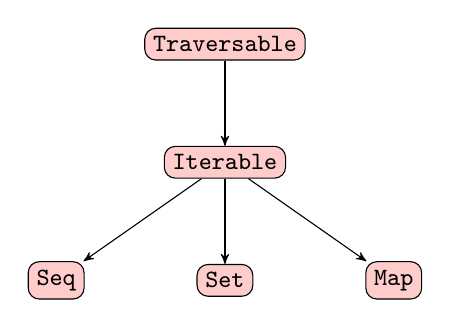
\begin{tikzpicture}[sibling distance=6.1em,->,>=stealth', inner sep=3pt, %scale=0.5,
  every node/.style = {shape=rectangle, draw, align=center,font=\small\ttfamily},
  class/.style = {fill=blue!20},
  trait/.style = {rounded corners, fill=red!20}]
  \node[trait] {Traversable}
    child { node[trait] {Iterable}
      child { node[trait] {Seq}
       }
      child { node[trait] {Set}
      }
      child { node[trait] {Map}
      }
    };
\end{tikzpicture}

\columnbreak

{\SlideFontTiny

\code{Traversable} har metoder som är implementerade med hjälp av: \\
\code{def foreach[U](f: Elem => U): Unit}\\

\vspace{1em}\code{Iterable} har metoder som är implementerade med hjälp av: \\
\code{def iterator: Iterator[A] }

}

\begin{itemize}\SlideFontTiny
\item[] \code{Seq}: ordnade i sekvens
\item[] \code{Set}: unika element
\item[] \code{Map}: par av (nyckel, värde)
\end{itemize}


\end{multicols}

{\SlideFontSmall Samlingen \Emph{\texttt{Vector}} är en \code{Seq} som är en \code{Iterable} som är en \code{Traversable}. \\ \vspace{0.5em}\pause
De konkreta samlingarna är uppdelade i dessa paket:\\
\code{scala.collection.immutable} \hfill som är \Emph{automatiskt} importerade\\
\code{scala.collection.mutable}  \hfill som \Alert{måste importeras} explicit\\\pause
(undantag: primitiva \code{scala.Array} som är automatiskt synlig)
}
\end{Slide}





% \begin{Slide}{Hierarki av samlingar i scala.collection}\SlideFontTiny
% \includegraphics[width=0.95\textwidth]{../img/collection/collection-traits}\\
% %\noindent Läs mer om Scalas samlingar här: \\
% \url{http://docs.scala-lang.org/overviews/collections/overview}
% \end{Slide}




\Subsection{Mängd} %%%%%%%%%%%%%%%%%%%%%%%%%%%%%%%%%%%%%%%%%%%%%%%%%%%%%%

\Subsection{Nyckel-värde-tabell} %%%%%%%%%%%%%%%%%%%%%%%%%%%%%%%%%%%%%%%%




\Subsection{\texttt{scala.collection}}




\begin{Slide}{Mer specifika samlingstyper i \texttt{scala.collection}}
Det finns \Alert{mer specifika} \Emph{subtyper} av \code{Seq}, \code{Set} och \code{Map}:
\\ \vspace{1em}

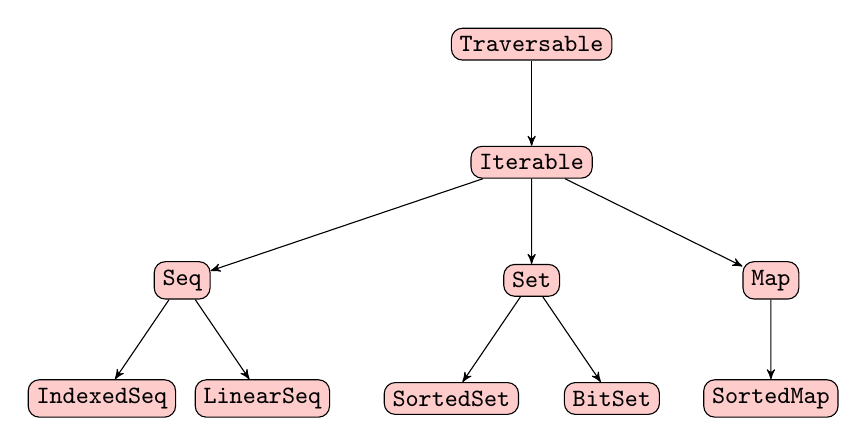
\begin{tikzpicture}[sibling distance=5.8em,->,>=stealth', inner sep=3pt, %scale=0.5,
  every node/.style = {shape=rectangle, draw, align=center,font=\small\ttfamily},
  class/.style = {fill=blue!20},
  trait/.style = {rounded corners, fill=red!20}]
  \node[trait] {Traversable}
    child { node[trait] {Iterable}
      child { node[trait, xshift=-2.4cm] {Seq}
        child { node[trait] {IndexedSeq} }
        child { node[trait] {LinearSeq} }
       }
      child { node[trait, yshift=-0.0cm] {Set}
        child { node[trait] {SortedSet} }
        child { node[trait] {BitSet} }
      }
      child { node[trait, xshift=1.0cm] {Map}
        child { node[trait] {SortedMap} }
      }
    };
\end{tikzpicture}

\vspace{0.5em}
\Emph{\texttt{Vector}} är en \Alert{\texttt{IndexedSeq}} medan
\Emph{\texttt{List}} är en \Alert{\texttt{LinearSeq}}.
\end{Slide}

\begin{Slide}{Några oföränderliga och förändringsbara sekvenssamlingar}\SlideFontSmall
\begin{tabular}{r l l}
\texttt{scala.collection.\Emph{immutable}.Seq.} & & \\
 & \code|IndexedSeq.| & \\
 & & \Emph{\texttt{Vector}} \\
 & & \Emph{\texttt{Range}} \\
 & \code|LinearSeq.| & \\
 & & \Emph{\texttt{List}} \\
   & & \Emph{\texttt{Queue}} \\

\texttt{scala.collection.\Alert{mutable}.Seq.} & & \\
 & \code|IndexedSeq.| & \\
 & & \Alert{\texttt{ArrayBuffer}} \\
 & & \Alert{\texttt{StringBuilder}} \\
 & \code|LinearSeq.| & \\
 & & \Alert{\texttt{ListBuffer}} \\
   & & \Alert{\texttt{Queue}} \\
\end{tabular}

Studera samlingars egenskaper här: \href{http://docs.scala-lang.org/overviews/collections/overview}{docs.scala-lang.org/overviews/collections/overview}
\end{Slide}




\begin{Slide}{Använda \texttt{iterator}}\SlideFontSmall
Med en \code{iterator} kan man \Emph{iterera} med \code{while} över alla element, men endast \Alert{en   gång}; sedan är iteratorn ''förbrukad''. (Men man kan be om en ny.)
\begin{REPL}
scala> val xs = Vector(1,2,3,4)
xs: scala.collection.immutable.Vector[Int] = Vector(1, 2, 3, 4)

scala> val it = xs.iterator
it: scala.collection.immutable.VectorIterator[Int] = non-empty iterator

scala> while (it.hasNext) print(it.next)
1234

scala> it.hasNext
res1: Boolean = false

scala> it.next
java.util.NoSuchElementException: reached iterator end
  at scala.collection.immutable.VectorIterator.next(Vector.scala:674)
\end{REPL}
\Emph{Normalt} behöver man \Alert{inte} använda \code{iterator}: det finns oftast färdiga metoder som gör det man vill, till exempel \code{foreach}, \code{map}, \code{sum}, \code{min} etc.
\end{Slide}





\begin{Slide}{Några användbara metoder på samlingar}\SlideFontTiny
\begin{tabular}{r r l}\hline
\texttt{\Emph{Traversable}}
  & \code|xs.size| & antal elementet \\
  & \code|xs.head| & första elementet \\
  & \code|xs.last| & sista elementet \\
  & \code|xs.take(n)| & ny samling med de första n elementet \\
  & \code|xs.drop(n)| & ny samling utan de första n elementet \\
  & \code|xs.foreach(f)| & gör \code|f| på alla element, returtyp \code|Unit|\\
  & \code|xs.map(f)| & gör \code|f| på alla element, ger ny samling \\
  & \code|xs.filter(p)| & ny samling med bara de element där p är sant\\
  & \code|xs.groupBy(f)| & ger en \code|Map| som grupperar värdena enligt f\\
  & \code|xs.mkString(",")| & en kommaseparerad sträng med alla element\\ \hline

\texttt{\Emph{Iterable}}
  & \code|xs.zip(ys)| & ny samling med par (x, y); ''zippa ihop'' xs och ys \\
  & \code|xs.zipWithIndex| & ger en \code|Map| med par (x, index för x) \\
  & \code|xs.sliding(n)| & ny samling av samlingar genom glidande ''fönster''\\ \hline

\texttt{\Emph{Seq}}
  & \code|xs.length| & samma som \code|xs.size| \\
  & \code|xs :+ x| & ny samling med x sist efter xs \\
  & \code|x +: xs| & ny samling med x före xs \\ \hline

\end{tabular}

\pause
\vspace{0.5em}\Emph{Minnesregel} för \code{+:} och \code{:+  } \Alert{Colon on the collection side}

\pause
Prova fler samlingsmetoder ur snabbreferensen: ~~\url{http://cs.lth.se/quickref}
\end{Slide}



\begin{Slide}{Använda samlingsmetoder}
\begin{REPL}
scala> val tal = Vector(1,4,7,9,42)
tal: scala.collection.immutable.Vector[Int] = Vector(1, 4, 7, 9, 42)

scala> val jämna = tal.filter(_ % 2 == 0)
jämna: scala.collection.immutable.Vector[Int] = Vector(4, 42)

scala> val xs = Vector(("Kim","Smith"), ("Kim", "Jones"), ("Robin", "Smith"))
xs: scala.collection.immutable.Vector[(String, String)] = Vector((Kim,Smith), (Kim,Jones), (Robin,Smith))

scala> val grupperaEfterFörnamn = xs.groupBy(_._1)
grupperaEfterFörnamn: Map[String,Vector[(String, String)]] =
Map(Kim -> Vector((Kim,Smith), (Kim,Jones)), Robin -> Vector((Robin,Smith)))

scala> val grupperaEfterEfternamn = xs.groupBy(_._2)
grupperaEfterEfternamn: Map[String,Vector[(String, String)]] =
Map(Jones -> Vector((Kim,Jones)), Smith -> Vector((Kim,Smith), (Robin,Smith)))

\end{REPL}
\end{Slide}




\begin{Slide}{scala.collection.immutable}
\includegraphics[width=0.82\textwidth]{../img/collection/collection-immutable}
\includegraphics[width=0.33\textwidth]{../img/collection/collection-legend}
\end{Slide}


\begin{Slide}{scala.collection.mutable}
\includegraphics[width=1.05\textwidth]{../img/collection/collection-mutable}
\end{Slide}


\begin{Slide}{Strängar är implicit en \texttt{IndexedSeq[Char]}}\SlideFontSmall
Det finns en så kallad \Emph{implicit konvertering} mellan \code{String} och \code{IndexedSeq[Char]} vilket gör att \Alert{alla samlingsmetoder på \texttt{Seq} även funkar på strängar} och även flera andra smidiga strängmetoder erbjuds \Alert{utöver} de som finns i \href{http://docs.oracle.com/javase/8/docs/api/java/lang/String.html}{\code{java.lang.String}} genom klassen \href{http://www.scala-lang.org/api/current/#scala.collection.immutable.StringOps}{\code{StringOps}}.

\vspace{0.5em}
\begin{REPLnonum}
scala> "hej".  //tryck på TAB och se alla strängmetoder
\end{REPLnonum}
Detta är en stor fördel med Scala jämfört med många andra språk, som har strängar som inte kan allt som andra sekvenssamlingar kan.
\end{Slide}


\begin{Slide}{\texttt{Vector} eller \texttt{List}?}\SlideFontTiny
{\href{http://stackoverflow.com/questions/6928327/when-should-i-choose-vector-in-scala}{stackoverflow.com/questions/6928327/when-should-i-choose-vector-in-scala}}

\begin{enumerate}
\item If we only need to transform sequences by operations like map, filter, fold etc: basically it does not matter, we should program our algorithm generically and might even benefit from accepting parallel sequences. For sequential operations List is probably a bit faster. But you should benchmark it if you have to optimize.

\item If we need a lot of random access and different updates, so we should use vector, list will be prohibitively slow.

\item If we operate on lists in a classical functional way, building them by prepending and iterating by recursive decomposition: use list, vector will be slower by a factor 10-100 or more.

\item If we have an performance critical algorithm that is basically imperative and does a lot of random access on a list, something like in place quick-sort: use an imperative data structure, e.g. ArrayBuffer, locally and copy your data from and to it.
\end{enumerate}
{\href{http://stackoverflow.com/questions/20612729/how-does-scalas-vector-work}{stackoverflow.com/questions/20612729/how-does-scalas-vector-work}}\\
Mer om tids- och minneskomplexitet i fördjupningskursen och senare kurser.
\end{Slide}



\begin{Slide}{Mängd: snabb innehållstest, garanterat dubblettfri}\SlideFontSmall
En \Emph{mängd} \Eng{set} är en samling som \Alert{inte} kan innehålla \Alert{dubbletter} och som är snabb på att avgöra om ett element \Alert{finns eller inte} i mängden.

\begin{REPL}
scala> var veg = Set.empty[String]
veg: scala.collection.immutable.Set[String] = Set()

scala> veg = veg + "Gurka"
veg: scala.collection.immutable.Set[String] = Set(Gurka)

scala> veg = veg ++ Set("Broccoli", "Tomat", "Gurka")
veg: scala.collection.immutable.Set[String] = Set(Gurka, Broccoli, Tomat)

scala> veg.contains("Gurka")
res0: Boolean = true

scala> veg.apply("Gurka")   // samma som contains
res1: Boolean = true

scala> veg("Morot")
res2: Boolean = false
\end{REPL}

\end{Slide}

\begin{Slide}{Den fantastiska nyckel-värde-tabellen \texttt{Map}}\SlideFontSmall
\begin{itemize}
\item En \Emph{nyckel-värde-tabell} \Eng{key-value table} är en slags generaliserad vektor där man kan ''indexera'' med godtycklig typ.

\item Kallas öven \href{https://sv.wikipedia.org/wiki/Hashtabell}{\Emph{hashtabell}} \Eng{hash table}, \Emph{lexikon} \Eng{dictionary} eller kort och gott \Emph{mapp} \Eng{map},

\item En hashtabell är en \Emph{samling av par}, där varje par består av en \Alert{unik} \Emph{nyckel} och ett tillhörande \Emph{värde}.

\item Om man vet nyckeln kan man få fram värdet \Alert{snabbt}, på liknande sätt som indexering sker i en vektor om man vet heltalsindex.

\item Denna datastruktur är \Alert{mycket användbar} och liknar en enkel databas.
\end{itemize}
\begin{REPL}
scala> val födelse = Map("C" -> 1972,  "C++" -> 1983, "C#" -> 2000,
  "Scala" -> 2004, "Java" -> 1995, "Javascript" -> 1995, "Python" -> 1991)

födelse: scala.collection.immutable.Map[String,Int] = Map(Scala -> 2004, C# -> 2000, Python -> 1991, Javascript -> 1995, C -> 1972, C++ -> 1983, Java -> 1995)

scala> födelse.apply("Scala")
res0: Int = 2004

scala> födelse("Java")
res1: Int = 1995

\end{REPL}
\end{Slide}

\begin{Slide}{Exempel nyckel-värde-tabell}
\begin{REPL}
scala> val färg = Map("gurka" -> "grön", "tomat"->"röd", "aubergine"->"lila")
färg: scala.collection.immutable.Map[String,String] =
  Map(gurka -> grön, tomat -> röd, aubergine -> lila)

scala> färg("gurka")
res0: String = grön

scala> färg.keySet
res1: scala.collection.immutable.Set[String] = Set(gurka, tomat, aubergine)

scala> val ärGrönSak = färg.map(elem => (elem._1, elem._2 == "grön"))
ärGrönSak: Map[String,Boolean] = Map(gurka -> true, tomat -> false, aubergine -> false)

scala> val baklängesFärg = färg.mapValues(s => s.reverse)
baklängesFärg: Map[String,String] = Map(gurka -> nörg, tomat -> dör, aubergine -> alil)

\end{REPL}
\begin{itemize}
\item \code{xs.keySet} ger en mängd av alla nycklar
\item \code{xs.map(f)} mappar funktionen f på alla par av (key, value)
\item \code{xs.mapValues(f)} mappar funktionen f på alla värden
\end{itemize}

\end{Slide}

\begin{Slide}{Metoderna zipWithIndex, groupBy och mapValues}
\begin{REPL}
scala> val högaKort = Vector("Knekt", "Dam", "Kung", "Äss")

scala> val kortIndex = högaKort.zipWithIndex.toMap
kortIndex: Map[String,Int] = Map(Knekt -> 0, Dam -> 1, Kung -> 2, Äss -> 3)

scala> kortIndex("Kung") > kortIndex("Knekt")
res0: Boolean = true

scala> val xs = Vector(("Kim","Smith"), ("Kim", "Jones"), ("Robin", "Smith"))
xs: Vector[(String, String)] = Vector((Kim,Smith), (Kim,Jones), (Robin,Smith))

scala> val grupperaEfterFörnamn = xs.groupBy(_._1)
grupperaEfterFörnamn: Map[String,Vector[(String, String)]] =
Map(Kim -> Vector((Kim,Smith), (Kim,Jones)), Robin -> Vector((Robin,Smith)))

scala> val grupperaEfterEfternamn = xs.groupBy(_._2)
grupperaEfterEfternamn: Map[String,Vector[(String, String)]] =
Map(Jones -> Vector((Kim,Jones)), Smith -> Vector((Kim,Smith), (Robin,Smith)))

scala> val frekvens = xs.groupBy(_._1).mapValues(_.size)
frekvens: Map[String,Int] = Map(Kim -> 2, Robin -> 1)
\end{REPL}
\end{Slide}


\begin{Slide}{Speciella metoder på förändringsbara samlingar}\SlideFontSmall
Både \code{Set} och \code{Map} finns i \Alert{förändringsbara} varianter med extra metoder för uppdatering av innehållet ''på plats'' utan att nya samlingar skapas.
\begin{REPL}
scala> import scala.collection.mutable

scala> val ms = mutable.Set.empty[Int]
ms: scala.collection.mutable.Set[Int] = Set()

scala> ms += 42
res0: ms.type = Set(42)

scala> ms += (1, 2, 3, 1, 2, 3); ms -= 1
res1: ms.type = Set(2, 42, 3)

scala> ms.mkString("Mängd: ", ", ", s" Antal: ${ms.size}")
res2: String = Mängd: 1, 2, 42, 3 Antal: 4

scala> val ordpar = mutable.Map.empty[String, String]
scala> ordpar += ("hej" -> "svejs", "abra" -> "kadabra", "ada" -> "lovelace")
scala> println(ordpar("abra"))
kadabra
\end{REPL}
\end{Slide}

\begin{Slide}{Fler exempel på samlingsmetoder}
Exempel: räkna bokstäver i ord.  \\
Undersök vad som händer i REPL:
\begin{Code}[basicstyle=\SlideFontSize{9}{13}\ttfamily]
val ord = "sex laxar i en laxask sju sjösjuka sjömän"
val uppdelad = ord.split(' ').toVector
val ordlängd = uppdelad.map(_.length)
val ordlängdMap = uppdelad.map(s => (s, s.size)).toMap
val grupperaEfterFörstaBokstav = uppdelad.groupBy(s => s(0))
val bokstäver = ord.toVector.filter(_ != ' ')
val antalX = bokstäver.count(_ == 'x')
val grupperade = bokstäver.groupBy(ch => ch)
val antal = grupperade.map(kv => (kv._1, kv._2.size))
val sorterat = antal.toVector.sortBy(_._2)
val vanligast = antal.maxBy(_._2)
\end{Code}
\end{Slide}


\begin{Slide}{Jobba med föränderlig samling lokalt; \\ returnera oföränderlig samling när du är klar}
\SlideFontSmall
Om du vill implementera en imperativ algoritm med en föränderlig samling:\\
Gör gärna detta \Alert{lokalt} i en \Alert{förändringsbar} samling och returnera sedan en \Emph{oföränderlig} samling, genom att köra t.ex. \code{toSet} på en mängd, eller \code{toMap} på en hashtabell, eller \code{toVector} på en \code{ArrayBuffer} eller \code{Array}.

\begin{REPL}
scala> :paste
def kastaTärningTillsAllaUtfallUtomEtt(sidor: Int = 6) = {
  val s = scala.collection.mutable.Set.empty[Int]
  var n = 0
  while (s.size < sidor - 1) {
    s += (math.random * sidor + 1).toInt
    n += 1
  }
  (n, s.toSet)
}
scala> kastaTärningTillsAllaUtfallUtomEtt()
res0: (Int, scala.collection.immutable.Set[Int]) = (13,Set(5, 1, 6, 2, 3))

\end{REPL}

\end{Slide}

%!TEX encoding = UTF-8 Unicode
%!TEX root = ../lect-w07.tex


\Subsection{Läsa från fil och URL}

\begin{Slide}{Serialisering och deserialisering}
\begin{itemize}
  \item Att \Emph{serialisera} innebär att \Alert{koda objekt} i minnet till en avkodningsbar \Alert{sekvens av symboler}, som kan lagras t.ex. i en fil på din hårddisk.
  \item Att \Emph{de-serialisera} innebär att \Alert{avkoda en sekvens av symboler}, t.ex. från en fil, och \Alert{återskapa objekt} i minnet.
\end{itemize}
\end{Slide}


\begin{Slide}{Läsa från fil och URL}
I paketet \code{scala.io} finns singelobjektet \code{Source} med metoderna \code{fromFile} och \code{fromUrl} för läsning från fil resp. från  URL\footnote{URL = Universal Resource Locator}, som börjar t.ex. med \code{http://}
\begin{Code}
def läsFrånFil(filnamn: String) = scala.io.Source.fromFile(filnamn).mkString

def läsRaderFrånFil(filnamn: String): Vector[String] =
  scala.io.Source.fromFile(filnamn).getLines.toVector

def läsFrånWebbsida(url: String) = scala.io.Source.fromURL(url).mkString

def läsRaderWebbsida(url: String, kodning: String = "UTF-8"): Vector[String] =
  scala.io.Source.fromURL(url, kodning).getLines.toVector

\end{Code}
Se exempel på veckans övning.
\end{Slide}


\begin{Slide}{Fördjupning: singelobjektet Disk}
Se fördjupningsuppgift övning \texttt{lookup}:
\scalainputlisting[basicstyle=\ttfamily\SlideFontSize{6}{7.5}]{../compendium/examples/Disk.scala}
\end{Slide}

%%!TEX encoding = UTF-8 Unicode
%!TEX root = ../lect-w07.tex

\ifkompendium\else

% \Subsection{Grumligtlådan}

% \begin{Slide}{Grumligtlådan}
%   \Alert{OM} du har något koncept i kursen som är \Alert{extra} ''grumligt'' så skriv ner det på en lapp i lådan som går runt. 
% \end{Slide}

% \begin{Slide}{Grumligtlådan: topplista med ämnen 2017}
% \begin{multicols}{2}
% \begin{verbatim}
%   om kursen       : 14
%   klass           : 9
%   this            : 7
%   filstruktur     : 5
%   pluggteknik     : 4
%   case-klass      : 4
%   registrera      : 3
%   filtrera        : 3
%   copy            : 3
%   tupel           : 2
%   konstruktor     : 2
%   iterera         : 2
%   fabriksmetod    : 2
%   synlighet       : 1
%   skuggning       : 1
%   sidoeffekt      : 1
%   Seq[T]          : 1
%   sekvenser       : 1
%   sats/uttryck    : 1
%   lambda          : 1
%   kompanjonsobj   : 1
%   högre ordn funk : 1
%   funktion        : 1
%   curry-funktion  : 1
% \end{verbatim}
% \end{multicols}
% \end{Slide}




% \begin{Slide}{Grumligtlådan: lajvkodning}
% Lajvkodning enligt begrepp i lådan utifrån denna klass:
% \begin{Code}[basicstyle=\ttfamily\SlideFontSize{12}{14}]
% class Frog(var n: Int) { def hop = n += 1 }
% \end{Code}
% \includegraphics[width=0.6\textwidth]{../img/frog}
% \end{Slide}

\fi



%!TEX encoding = UTF-8 Unicode

%!TEX root = ../compendium2.tex

\chapter{Mönster, Undantag}\label{chapter:W08}
\begin{itemize}[nosep]
\item match
\item Option
\item null
\item try
\item catch
\item Try
\item unapply
\end{itemize}
\clearpage\section{Teori}
%!TEX encoding = UTF-8 Unicode
%!TEX root = ../lect-w08.tex

%%%

\Subsection{Veckans labb: \texttt{life}}

\begin{Slide}{Veckans labb: \texttt{life}}
\begin{minipage}{0.52\textwidth}
  \setlength{\leftmargini}{0pt}

\begin{itemize}
  \SlideFontSmall
\item Universum är en binär matris av \Emph{celler} där \Emph{levande} celler representeras med \code{true} och \Alert{döda} med \code{false}.
\item Följande regler gäller för \Emph{nästa generation} celler i universum:
\begin{itemize}\SlideFontTiny
  \item \textbf{Fortlevnad}: en levande cell med 2 eller 3 grannar \Emph{lever vidare}
  \item \textbf{Död}: en levande cell med färre än 2 eller fler än 3 grannar \Alert{dör}
  \item \textbf{Födelse}: en död cell med exakt tre grannar föds
\end{itemize}
\item Övning \code{matrices} uppgift 5: skapa en generisk \code{case class Matrix[T]}
\item På labben: använd \code{Matrix[Boolean]}
\end{itemize}

\end{minipage}%
\begin{minipage}{0.5\textwidth}
  \includegraphics[width=1.0\textwidth]{../img/glider-blinker-block}

  \begin{itemize}\SlideFontTiny
  \item Du ska simulera \emph{Game of Life} i ett \code{introprog.PixelWindow}
  \item Fördjupning:\\{\SlideFontTiny\url{https://en.wikipedia.org/wiki/Conway%27s_Game_of_Life}}
  \end{itemize}
\end{minipage}%

\end{Slide}






\Subsection{Matriser}

\begin{Slide}{Vad är en matris?}\SlideFontSmall
\begin{itemize}

\item En \Emph{matris} inom \Alert{matematiken} innehåller \Emph{rader} och \Emph{kolumner}\footnote{även kallade \emph{kolonner}} med tal.

\item I en \Alert{matematisk} matris har alla rader \Emph{lika många} element och

\item även alla kolumner har \Emph{lika många} element.

\item En matris av dimension $2\times{}5$ har $2 \cdot 5 = 10$ stycken element.

\item Exempel på en matematisk matris av dimension $2\times{}5$:
\[
M_{2,5}=
  \begin{pmatrix}
    5 & 2 & 42 & 4 & 5 \\
    3 & 4 & 18 & 6 & 7
  \end{pmatrix}
\]
\end{itemize}
\end{Slide}

\begin{Slide}{Indexering i en matris}\SlideFontSmall
\begin{itemize}

  \item En matris av dimension $m\times{}n$ har $m \cdot n$ stycken element.

  \item En matris $A_{m,n}$ av dimension $m\times{}n$ ritas inom matematiken ofta så här:

  \[
  A_{m,n} =
   \begin{pmatrix}
    a_{1,1} & a_{1,2} & \cdots & a_{1,n} \\
    a_{2,1} & a_{2,2} & \cdots & a_{2,n} \\
    \vdots  & \vdots  & \ddots & \vdots  \\
    a_{m,1} & a_{m,2} & \cdots & a_{m,n}
   \end{pmatrix}
  \]


\item Matrisindexering inom matematiken sker ofta från $1$, men ofta från $0$ i datorprogram.

\item Vad har talet $42$ för index i matrisen $M_{2,5}$ nedan?
\begin{itemize}\SlideFontTiny
  \item[--] Inom matematiken?
  \item[--] I Scala och Java och många andra språk?

  \[
  M_{2,5}=
    \begin{pmatrix}
      5 & 2 & 42 & 4 & 5 \\
      3 & 4 & 18 & 6 & 7
    \end{pmatrix}
  \]
\end{itemize}
\end{itemize}
\end{Slide}

\begin{Slide}{Hur skapa matriser?}
  \setlength{\leftmargini}{0pt}

  \begin{itemize}
  \item Inom programmering används ordet \Emph{matris} ofta för att beteckna en \Alert{nästlad struktur} i två dimensioner. Exempel:
  \begin{itemize}
   \item \Emph{Oföränderliga} sekvenser, t.ex. \code{Vector[Vector[Int]]} \\
   \code{val xss = Vector(Vector(0, 0, 0), Vector(0, 0, 0))} eller enklare: \\
      \code{val xss = Vector.fill(2,3)(0)}

    \item \Alert{Föränderliga} sekvens, t.ex. \code{Array[Array[Int]]} \\
    \code{val yss = Array(Array(0, 0, 0), Array(0, 0, 0))} eller enklare: \\
       \code{val yss = Array.fill(2,3)(0)}

  \end{itemize}

\end{itemize}
\end{Slide}

\begin{Slide}{Hur indexera i matriser?}
En matris med array av arrayer:
\begin{REPL}
scala> val xss = Array(Array(5,2,42,4,5),Array(3,4,18,6,7))
xss: Array[Array[Int]] = Array(Array(5, 2, 42, 4, 5), Array(3, 4, 18, 6, 7))
\end{REPL}
\pause
Man indexerar i en nästlad sekvens med upprepad \code{apply}:
\begin{REPL}
scala> xss(0)(2)
res0: ???

scala> xss.apply(0).apply(2)
res1: ???

scala> xss(0)
res2: ???
\end{REPL}
Övning: Vad är typ och värde vid \code{???} ovan?
\end{Slide}

\begin{Slide}{Hur indexera i matriser?}
En matris med array av arrayer:
\begin{REPL}
scala> val xss = Array(Array(5,2,42,4,5),Array(3,4,18,6,7))
xss: Array[Array[Int]] = Array(Array(5, 2, 42, 4, 5), Array(3, 4, 18, 6, 7))
\end{REPL}

Man indexerar i en nästlad sekvens med upprepad \code{apply}:
\begin{REPL}
scala> xss(0)(2)
res0: Int = 42

scala> xss.apply(0).apply(2)
res1: Int = 42

scala> xss(0)
res2: Array[Int] = Array(5, 2, 42, 4, 5)
\end{REPL}
Övning: Rita en bild av minnet som referensen \code{xss} refererar till.

\end{Slide}

\begin{Slide}{Uppdatering av en förändringsbar nästlad struktur}
Man kan förändra en array av arrayer ''på plats'' med tilldelning:
\begin{REPL}
scala> val xss = Array(Array(5,2,42,4,5),Array(3,4,18,6,7))

scala> xss(0)(0) = 100

scala> xss
res0: ???

scala> xss(0)(2) = xss(0)(2) - 1

scala> xss
res1: ???

scala> xss(1) = Array.fill(5)(-1)

scala> xss
res2: ???
\end{REPL}
\end{Slide}

\begin{Slide}{Uppdatering av en förändringsbar nästlad struktur}
Man kan förändra en array av arrayer ''på plats'' med tilldelning:
\begin{REPL}
scala> val xss = Array(Array(5,2,42,4,5),Array(3,4,18,6,7))

scala> xss(0)(0) = 100

scala> xss
res0: Array[Array[Int]]=Array(Array(100, 2, 42, 4, 5), Array(3, 4, 18, 6, 7))

scala> xss(0)(2) = xss(0)(2) - 1

scala> xss
res1: Array[Array[Int]]=Array(Array(100, 2, 41, 4, 5), Array(3, 4, 18, 6, 7))

scala> xss(1) = Array.fill(5)(-1)

scala> xss
res2: Array[Array[Int]]=Array(Array(100, 2, 41, 4, 5), Array(-1,-1,-1,-1,-1))
\end{REPL}
\end{Slide}

\begin{Slide}{Några olika sätt att skapa förändringsbara matriser}\SlideFontSmall
Det jobbiga, primitiva sättet:
\begin{REPL}
scala> val xss = new Array[Array[Int]](2)
xss: Array[Array[Int]] = Array(null, null)

scala> for (i <- xss.indices) {xss(i) = new Array[Int](5)}

scala> xss
res0: Array[Array[Int]] = Array(Array(0, 0, 0, 0, 0), Array(0, 0, 0, 0, 0))

scala> println(xss)
[[I@196a99d0
\end{REPL}
Enklare sätt:
\begin{REPL}
scala> val xss = Array.ofDim[Int](2,5)
xss: Array[Array[Int]] = Array(Array(0, 0, 0, 0, 0), Array(0, 0, 0, 0, 0))
\end{REPL}
Enklare och tydligare sätt, där initialvärdet anges explicit:
\begin{REPL}
scala> val xss = Array.fill(2,5)(0)
xss: Array[Array[Int]] = Array(Array(0, 0, 0, 0, 0), Array(0, 0, 0, 0, 0))
\end{REPL}

\end{Slide}

\begin{Slide}{Exempel på skapande av oföränderlig nästlad struktur}\SlideFontSmall
Om du kan beräkna initialvärde direkt, använd \code{Vector.fill}:\\
{\SlideFontTiny\code{def fill[A](n1: Int, n2: Int)(elem: => A): Vector[Vector[A]]}}
\begin{REPL}
scala> Vector.fill(2,5)(scala.util.Random.nextInt(6) + 1)
res0:
  typ???
  värde???

\end{REPL}
Om du kan beräkna initialvärde ur index, använd \code{Vector.tabulate}:\\
{\SlideFontTiny\code{def tabulate[A](n1: Int, n2: Int)(f: (Int, Int) => A): Vector[Vector[A]]}}
\begin{REPL}
scala> Vector.tabulate(5,2)((x,y) => x + y + 1)
res1:
  typ???
  värde???

\end{REPL}
\end{Slide}

\begin{Slide}{Exempel på skapande av oföränderlig nästlad struktur}\SlideFontSmall
Om du kan beräkna initialvärde direkt, använd \code{Vector.fill}:\\
{\SlideFontTiny\code{def fill[A](n1: Int, n2: Int)(elem: => A): Vector[Vector[A]]}}
\begin{REPL}
scala> Vector.fill(2,5)(scala.util.Random.nextInt(6) + 1)
res0: Vector[Vector[Int]] =
  Vector(Vector(1, 2, 6, 2, 1), Vector(1, 4, 3, 3, 2))

\end{REPL}
Om du kan beräkna initialvärde ur index, använd \code{Vector.tabulate}:\\
{\SlideFontTiny\code{def tabulate[A](n1: Int, n2: Int)(f: (Int, Int) => A): Vector[Vector[A]]}}
\begin{REPL}
scala> Vector.tabulate(5,2)((x,y) => x + y + 1)
res1: Vector[Vector[Int]] =
  Vector(Vector(1,2), Vector(2,3), Vector(3,4), Vector(4,5), Vector(5,	6))

\end{REPL}
\end{Slide}



\begin{Slide}{Uppdatering av en oföränderlig nästlad struktur}\SlideFontSmall
Uppdatering av endimensionell struktur med \code{xs.updated}:\\
{\SlideFontTiny\code{def updated[A](index: Int, elem: A): Vector[A]} }
\begin{REPL}
scala> var xs = Vector.tabulate(5)(x => x + 1)
xs: typ??? = värde???

scala> xs = xs.updated(1, 42)
xs: typ??? = värde???
\end{REPL}

Uppdatering av nästlad struktur i två dimensioner:
\begin{REPL}
scala> var xss = Vector.tabulate(2, 5)((x,y) => x + y + 1)
xss:
  typ??? =
  värde???

scala> xss = xss.updated(0, xss(0).updated(1, 42))
xss:
  typ??? =
  värde???
\end{REPL}

\end{Slide}



\begin{Slide}{Uppdatering av en oföränderlig nästlad struktur}\SlideFontSmall
Uppdatering av endimensionell struktur med \code{xs.updated}:\\
{\SlideFontTiny\code{def updated[A](index: Int, elem: A): Vector[A]} }
\begin{REPL}
scala> var xs = Vector.tabulate(5)(x => x + 1)
xs: Vector[Int] = Vector(1, 2, 3, 4, 5)

scala> xs = xs.updated(1, 42)
xs: Vector[Int] = Vector(1, 42, 3, 4, 5)
\end{REPL}

Uppdatering av nästlad struktur i två dimensioner:
\begin{REPL}
scala> var xss = Vector.tabulate(2, 5)((x,y) => x + y + 1)
xss: Vector[Vector[Int]] =
  Vector(Vector(1, 2, 3, 4, 5), Vector(2, 3, 4, 5, 6))

scala> xss = xss.updated(0, xss(0).updated(1, 42))
xss:
  Vector[Vector[Int]] =
  Vector(Vector(1, 42, 3, 4, 5), Vector(2, 3, 4, 5, 6))
\end{REPL}

\end{Slide}


\begin{Slide}{Iterera över nästlad struktur}\SlideFontSmall
Behandling av nästlade strukturer kräver ofta algoritmer med nästlad iterering. \\
Exempel: iterera med nästlad \code{for}-sats för utskrift av denna matris\\
\code{val xss = Vector.tabulate(2,5)((x,y) => x + y + 1)}
\pause
\begin{REPL}
scala> for ??? do
         for ??? do 
           print(xss(i)(j))
           print(" ")
         println

1 2 3 4 5
2 3 4 5 6
\end{REPL}
Övning: \\Vad ska det stå vid \code{???} för att alla element ska skrivas ut?
\end{Slide}

\begin{Slide}{Iterera över nästlad struktur}\SlideFontSmall
  \vspace{1em}
  Behandling av nästlade strukturer kräver ofta algoritmer med nästlad iterering. \\
  Exempel: iterera med nästlad \code{for}-sats för utskrift av denna matris \\
  \code{val xss = Vector.tabulate(2,5)((x,y) => x + y + 1)}

  \begin{REPL}
scala> for xs <- xss do
         for x <- xs do 
           print(x)
           print(" ")
         end for
         println()
       end for

1 2 3 4 5
2 3 4 5 6
\end{REPL}
Övning: skriv ut matrisen med nästlad \code{foreach}\\
\pause
\begin{Code}
xss.foreach { xs => 
  xs.foreach { x => print(x); print(" ") }
  println()
}
\end{Code}
\end{Slide}


\begin{Slide}{Övningsexempel: Yatzy}\SlideFontSmall
Skapa en funktion \code{roll} som ger utfallet av n st tärningskast:
\begin{REPL}
scala> import scala.util.Random

scala> def roll(n: Int): Vector[Int] = ???
\end{REPL}

Skapa en funktion \code{isYatzy} som ger \code{true} om alla utfall är lika:
\begin{REPL}
scala> def isYatzy(xs: Vector[Int]): Boolean = ???
\end{REPL}
Du kan anta att xs.length > 0\\
Tips: använd metoden xs.forall: \\
\code{def forall[A](p: A => Boolean): Boolean }
\end{Slide}


\begin{Slide}{Övningsexempel: Yatzy}\SlideFontSmall
Skapa en funktion \code{roll} som ger utfallet av n st tärningskast:
\begin{REPL}
scala> import scala.util.Random

scala> def roll(n: Int): Vector[Int] = Vector.fill(n)(Random.nextInt(6) + 1)
\end{REPL}

Skapa en funktion \code{isYatzy} som ger \code{true} om alla utfall är lika:
\begin{REPL}
scala> def isYatzy(xs: Vector[Int]): Boolean = xs.forall(x => x == xs(0))
\end{REPL}
Du kan anta att xs.length > 0\\
Tips: använd metoden xs.forall: \\
\code{def forall[A](p: A => Boolean): Boolean }
\end{Slide}

\begin{Slide}{Iterera över nästlad struktur: for-sats}\SlideFontSmall
Iterera med nästlad for-sats: (vad har xss för typ?)
\begin{REPL}
scala> val xss = Vector.fill(100)(roll(5))

scala> for (i <- ???) do 
         for (j <- ???) do
           print(s"($i)($j): ${xss(i)(j)} ")
         println(s" YATZY: ${isYatzy(xss(i))}")

(0)(0): 3 (0)(1): 6 (0)(2): 4 (0)(3): 4 (0)(4): 6  YATZY: false
(1)(0): 4 (1)(1): 1 (1)(2): 5 (1)(3): 2 (1)(4): 6  YATZY: false
(2)(0): 1 (2)(1): 3 (2)(2): 5 (2)(3): 6 (2)(4): 2  YATZY: false
(3)(0): 2 (3)(1): 1 (3)(2): 1 (3)(3): 5 (3)(4): 4  YATZY: false
(4)(0): 4 (4)(1): 4 (4)(2): 1 (4)(3): 6 (4)(4): 5  YATZY: false
(5)(0): 3 (5)(1): 3 (5)(2): 2 (5)(3): 3 (5)(4): 6  YATZY: false
(6)(0): 3 (6)(1): 6 (6)(2): 1 (6)(3): 1 (6)(4): 4  YATZY: false
(7)(0): 6 (7)(1): 2 (7)(2): 4 (7)(3): 4 (7)(4): 3  YATZY: false
(8)(0): 1 (8)(1): 5 (8)(2): 4 (8)(3): 2 (8)(4): 4  YATZY: false
(9)(0): 1 (9)(1): 1 (9)(2): 3 (9)(3): 6 (9)(4): 6  YATZY: false
(10)(0): 2 (10)(1): 5 (10)(2): 2 (10)(3): 4 (10)(4): 5  YATZY: false
(11)(0): 3 (11)(1): 4 (11)(2): 2 (11)(3): 5 (11)(4): 6  YATZY: false
...
\end{REPL}
\end{Slide}

\begin{Slide}{Iterera över nästlad struktur: for-sats}\SlideFontSmall
Iterera med nästlad for-sats: (xss är en \code{Vector[Vector[Int]]})
\begin{REPL}
scala> val xss = Vector.fill(100)(roll(5))

scala> for (i <- xss.indices) do 
         for (j <- xss(i).indices) do
           print(s"($i)($j): ${xss(i)(j)} ")
         println(s" YATZY: ${isYatzy(xss(i))}")

(0)(0): 3 (0)(1): 6 (0)(2): 4 (0)(3): 4 (0)(4): 6  YATZY: false
(1)(0): 4 (1)(1): 1 (1)(2): 5 (1)(3): 2 (1)(4): 6  YATZY: false
(2)(0): 1 (2)(1): 3 (2)(2): 5 (2)(3): 6 (2)(4): 2  YATZY: false
(3)(0): 2 (3)(1): 1 (3)(2): 1 (3)(3): 5 (3)(4): 4  YATZY: false
(4)(0): 4 (4)(1): 4 (4)(2): 1 (4)(3): 6 (4)(4): 5  YATZY: false
(5)(0): 3 (5)(1): 3 (5)(2): 2 (5)(3): 3 (5)(4): 6  YATZY: false
(6)(0): 3 (6)(1): 6 (6)(2): 1 (6)(3): 1 (6)(4): 4  YATZY: false
(7)(0): 6 (7)(1): 2 (7)(2): 4 (7)(3): 4 (7)(4): 3  YATZY: false
(8)(0): 1 (8)(1): 5 (8)(2): 4 (8)(3): 2 (8)(4): 4  YATZY: false
(9)(0): 1 (9)(1): 1 (9)(2): 3 (9)(3): 6 (9)(4): 6  YATZY: false
(10)(0): 2 (10)(1): 5 (10)(2): 2 (10)(3): 4 (10)(4): 5  YATZY: false
(11)(0): 3 (11)(1): 4 (11)(2): 2 (11)(3): 5 (11)(4): 6  YATZY: false
...
\end{REPL}
\end{Slide}


% \begin{Slide}{Iterera över nästlad struktur med nästlad foreach}\SlideFontSmall
% Iterera med nästlad foreach-sats:
% \begin{REPL}
% scala> val xss = Vector.tabulate(2,5)((x,y) => x + y + 1)

% xss.foreach{ xs => ??? ; println }

% 1 2 3 4 5
% 2 3 4 5 6
% \end{REPL}
% \end{Slide}


% \begin{Slide}{Iterera över nästlad struktur med nästlad foreach}\SlideFontSmall
% Iterera med nästlad foreach-sats:
% \begin{REPL}
% scala> val xss = Vector.tabulate(2,5)((x,y) => x + y + 1)

% xss.foreach{ xs => xs.foreach{ x => print(x + " ") }; println }

% 1 2 3 4 5
% 2 3 4 5 6
% \end{REPL}
% \end{Slide}


\begin{Slide}{Nästlade for-uttryck}\SlideFontSmall
Iterera med \Emph{nästlad for-yield}:\\
%Statisk typ: \code{IndexedSeq[IndexedSeq[[Int]]} \\
%Dynamisk typ: \code{Vector[Vector[[Int]]}

\begin{REPL}
scala> val xss = for (i <- 1 to 2) yield 
                   for (j <- 1 to 5) yield i + j + 1
                 
val xss: IndexedSeq[IndexedSeq[Int]] =
      ???

\end{REPL}
\pause Om man skriver så här får man en endimensionell struktur:
\begin{REPL}
scala> val xs = for (i <- 1 to 2; j <- 1 to 5) yield i + j + 1
val xs: IndexedSeq[Int] =
    ???

\end{REPL}
\end{Slide}

\begin{Slide}{Nästlade for-uttryck}\SlideFontSmall
Iterera med \Emph{nästlad for-yield}:\\
\begin{REPL}
scala> val xss = for (i <- 1 to 2) yield {
                   for (j <- 1 to 5) yield i + j + 1
                 }
val xss: IndexedSeq[IndexedSeq[Int]] =
    Vector(Vector(3, 4, 5, 6, 7), Vector(4, 5, 6, 7, 8))

\end{REPL}
\pause Om man skriver så här får man en endimensionell struktur:
\begin{REPL}
scala> val xs = for (i <- 1 to 2; j <- 1 to 5) yield i + j + 1
val xs: IndexedSeq[Int] =
    Vector(3, 4, 5, 6, 7, 4, 5, 6, 7, 8)

\end{REPL}
\end{Slide}



\begin{Slide}{Nästlade map-uttryck}\SlideFontSmall
Iterera med \Emph{nästlade map-uttryck}:\\
\begin{REPL}
scala> val xss = (1 to 2).map(i => (1 to 5).map(j => i + j + 1))
xss: IndexedSeq[IndexedSeq[Int]] =
      ???
\end{REPL}
\end{Slide}

\begin{Slide}{Nästlade map-uttryck}\SlideFontSmall
Iterera med \Emph{nästlade map-uttryck}:\\
\begin{REPL}
scala> val xss = (1 to 2).map(i => (1 to 5).map(j => i + j + 1))
xss: IndexedSeq[IndexedSeq[Int]] =
      Vector(Vector(3, 4, 5, 6, 7), Vector(4, 5, 6, 7, 8))
\end{REPL}
\end{Slide}



\ifkompendium\else
\begin{Slide}{Fallgrop: likhet av array}
\begin{REPL}
scala> Vector.fill(5, 2)(42) == Vector.fill(5, 2)(42)
val res0: ???

scala> Array.fill(5, 2)(42) == Array.fill(5, 2)(42)
val res1: ???
\end{REPL}
\end{Slide}
\fi

\begin{Slide}{Fallgrop: likhet av array}
\begin{REPL}
scala> Vector.fill(5, 2)(42) == Vector.fill(5, 2)(42)
val res0: Boolean = true

scala> Array.fill(5, 2)(42) == Array.fill(5, 2)(42)
val res1: Boolean = false  // AAAARRGH!!! :(
\end{REPL}
Primitiva arrayer har en equals-metod som ger referenslikhet, \Alert{inte} innehållslikhet. Och det fungerar följaktligen ej heller på nästlade strukturer. 
\end{Slide}

\ifkompendium\else
\begin{Slide}{Övning: Kolla likhet av array (uppfinner hjulet)}
\begin{Code}
def isEqual(xss: Array[Array[Int]], yss: Array[Array[Int]]) = 
  var i = 0
  var foundUnequal = false
  while ??? do                          // VILKET VILLKOR?
    var j = 0
    while ??? do                        // VILKET VILLKOR?
      if xss(i)(j) != yss(i)(j) then ???   // VAD SKA UPPDATERAS? 
      j += 1
    end while
    i += 1
  end while
  !foundUnequal
end isEqual
\end{Code}
\begin{REPL}
scala> val (xss, yss) = (Array.fill(5,2)(42), Array.fill(5,2)(42))

scala> isEqual(xss, yss)

scala> yss(4)(1) = 0

scala> isEqual(xss, yss)
\end{REPL}
\end{Slide}
\fi


\begin{Slide}{Övning: Kolla likhet av array (uppfinner hjulet)}
\begin{Code}
def isEqual(xss: Array[Array[Int]], yss: Array[Array[Int]]) = 
  var i = 0
  var foundUnequal = false
  while i < xss.length && !foundUnequal do
    var j = 0
    while j < xss(i).length && !foundUnequal do
      if xss(i)(j) != yss(i)(j) then foundUnequal = true
      j += 1
    end while
    i += 1
  end while
  !foundUnequal
end isEqual
\end{Code}
\begin{REPL}
scala> val (xss, yss) = (Array.fill(5,2)(42), Array.fill(5,2)(42))

scala> isEqual(xss, yss)  // true

scala> yss(4)(1) = 0

scala> isEqual(xss, yss)  // false
\end{REPL}
\end{Slide}

\begin{Slide}{Använd \texttt{sameElements} för test av innehållslikhet men bara på icke-nästlade arrayer}

  I Scala kan du använda metoden \code{sameElements} på arrayer för innehållslikhet, men det funkar \Alert{INTE} på nästlade strukturer.

\begin{REPL}
scala> val xs = Array(1,2,3)
xs: Array[Int] = Array(1, 2, 3)

scala> val ys = Array(1,2,3)
ys: Array[Int] = Array(1, 2, 3)

scala> xs.sameElements(ys)
res0: Boolean = true

scala> Array(Array(1)) sameElements Array(Array(1))  
res1: Boolean = false

\end{REPL}
\pause Använd i stället: \code{java.util.Arrays.deepEquals(xs, ys)}\\
men det kan då behövas \code{.asInstanceOf[Array[Object]]} på argumenten om kompilatorn inte klarar typkonverteringen.
\end{Slide}

% \begin{Slide}{Matris som Array med Array med heltal i Java}\SlideFontTiny
% \begin{CodeSmall}[language=Java]
% public class ArrayMatrix {

%     public static void showMatrix(int[][] m){
%         System.out.println("\n--- showMatrix ---");
%         for (int row = 0; row < m.length; row++){
%             for (int col = 0; col < m[row].length; col++) {
%                 System.out.print("[" + row + "]");
%                 System.out.print("[" + col + "] = ");
%                 System.out.print(m[row][col] + "; ");
%             }
%             System.out.println();
%         }
%     }

%     public static void main(String[] args) {
%         int[][] xss = new int[10][5];
%         showMatrix(xss);
%     }
% }
% \end{CodeSmall}
% \pause
% Övning: skriv en metod \code{fillRnd} som fyller en heltalsmatris med slumptal 1 till n:\\
% \pause
% \jcode|public static void fillRnd(int[][] m, int n){ /* ??? */ }| \\
% \pause
% Tips: använd en nästlad for-sats och detta uttryck: \\
% \jcode{(int) (Math.random() * n + 1) // (int) motsvarar Scalas asInstanceOf[Int]}

% \end{Slide}

\begin{Slide}{Om veckans övningar}\SlideFontSmall
\begin{itemize}
\item Träna på att iterera över nästlade strukurer

\item Fortsätt jobba med Yatzy-exemplet

\item träna på att skapa \Emph{imperativa} algoritmer: \\
lös \code{isYatzy} med \code{while}-sats 

\item Extrauppgift där du ska bygga ett enkelt yatzy-spel i terminalen (kunde varit en tentauppgift...)

\end{itemize}
\end{Slide}

% \begin{Slide}{Övning extrauppgift, utgör början på labb \code{survey}}\SlideFontSmall
%
% \begin{ScalaSpec}{Table}
% object Table {
%   /** Creates a new Table from fileName with columns split by sep */
%   def fromFile(fileName: String, separator: Char = ';'): Table = ???
% }
% case class Table(
%   data: Vector[Vector[String]],
%   headings: Vector[String],
%   sep: String){
%   /** A 2-tuple with (number of rows, number of columns) in data */
%   val dim: (Int, Int) = ???
%
%   /** The element in row r an column c of data, counting from 0 */
%   def apply(r: Int, c: Int): String = ???
%
%   /** The row-vector r in data, counting from 0 */
%   def row(r: Int): Vector[String]= ???
%
%   /** The column-vector c in data, counting from 0 */
%   def col(c: Int): Vector[String] = ???
%
%   /** A map from heading to index counting from 0 */
%   lazy val indexOfHeading: Map[String, Int] = ???
%
%   /** The column-vector with heading h in data */
%   def col(h: String): Vector[String] = ???
%
%   /** A vector with the distinct, sorted values of col with heading h */
%   def values(h: String): Vector[String] = ???
%
%   /** Headings and data with columns separated by sep */
%   override lazy val toString: String = ???
% }
% \end{ScalaSpec}
% \end{Slide}


% \begin{Slide}{Övn. fördjupn. uppg.: skapa en generisk matris-klass}\SlideFontSmall
% \vspace{-0.7em}
% \begin{Code}[basicstyle=\SlideFontSize{6}{6.8}\ttfamily\selectfont]
% case class Matrix[T](data: Vector[Vector[T]]){
%
%   def foreachRowCol(f: (Int, Int, T) => Unit): Unit =
%     for (r <- data.indices) {
%       for (c <- data(r).indices) {
%         f(r, c, data(r)(c))
%       }
%     }
%
%   def map[U](f: T => U): Matrix[U] = Matrix(data.map(_.map(f)))
%
%   /** The element at row r and column c */
%   def apply(r: Int, c: Int): T = ???
%
%   /** Gives Some[T](element) at index (r, c) if within index bounds, else None */
%   def get(r: Int, c: Int): Option[T] = ???
%
%   /** The row vector of row r */
%   def row(r: Int): Vector[T] = ???
%
%   /** The column vector of column c */
%   def col(c: Int): Vector[T] = ???
%
%   /** A new Matrix with element at row r and col c updated */
%   def updated(r: Int, c: Int, value: T): Matrix[T] = ???
% }
% object Matrix {
%   def fill[T](rowSize: Int, colSize: Int)(init: T): Matrix[T] =
%     new Matrix(Vector.fill(rowSize)(Vector.fill(colSize)(init)))
% }
% \end{Code}
% \end{Slide}

%!TEX encoding = UTF-8 Unicode
%!TEX root = ../lect-w08.tex

\Subsection{Typparametrar}



\begin{Slide}{Exempel: Icke-generisk case-klass med heltalsmatris}
  En \emph{icke-generisk} datastruktur har inga obundna typparametrar; alla typer är \Emph{konkreta} (alltså specifika). \\~\\ En icke-generisk case-class med en \code{Vector[Vector[Int]]}:
  \begin{Code}
  case class Matrix(data: Vector[Vector[Int]]):
    def apply(x: Int, y: Int): Int = data(x)(y)
  \end{Code}

  \begin{REPL}
  scala> Matrix(Vector(Vector(5, 2, 42, 4, 5),Vector(3, 4, 18, 6, 7)))
  res0: Matrix =
    Matrix(Vector(Vector(5, 2, 42, 4, 5), Vector(3, 4, 18, 6, 7)))
  \end{REPL}

\end{Slide}





\begin{Slide}{Exempel: Generisk case-klass med generell matris}
  En \emph{generisk} datastruktur har minst en obunden \Emph{typparameter} som kan bindas  till ett \Alert{konkret} \Emph{typargument}.
  
  \begin{Code}
  case class Matrix[T](data: Vector[Vector[T]]):
    def apply(x: Int, y: Int): T = data(x)(y)
  \end{Code}
  \code{Matrix} i exemplet ovan är en \Emph{generisk} case-class där \code{T} är obunden, eftersom \code{T} är en typparameter deklarerad inom \code{[]} \Alert{efter} klassens namn men \Alert{före} klassparameterlistan. \\

  \vspace{0.5em} Användning där \code{T} binds till \code{Int} via kompilatorns typhärledning:
  \begin{REPL}
  scala> Matrix(Vector(Vector(5, 2, 42, 4, 5),Vector(3, 4, 18, 6, 7)))
  res1: Matrix[Int] =
    Matrix(Vector(Vector(5, 2, 42, 4, 5), Vector(3, 4, 18, 6, 7)))
  \end{REPL}

\end{Slide}




\begin{Slide}{Vad är en typparameter?}\SlideFontSmall
  \setlength{\leftmargini}{0pt}

\begin{itemize}
\item En \Emph{typparameter} gör det möjligt att ge ett \Emph{typargument}.
\item Detta kallas \Emph{parametrisk polymorfism} \Eng{paramteric polymorphism}.
\item Exempel: \Emph{generisk} \Alert{funktion}:
\begin{Code}
def tnirp[A](x: A):Unit = println(x.toString.reverse)
\end{Code}
\pause
\item En \Emph{fri} typparameter kan bindas till vilken typ som helst.
\item Bindingen av typargument till typparametrar sker vid \Alert{kompileringstid}.
\item En typparameter är \Emph{fri} om den \Alert{inte} fått något värde, annars \Emph{bunden}. 
\pause
\item Exempel: \Emph{generisk} \Alert{klass} med \Emph{generiska} \Alert{metoder}:
\begin{Code}
class Cell[A](   // [A] är fri (måste bindas vid användning) 
    var value: A):                              // A är bunden
  def update(a: A): Unit = value = a            // A är bunden
  def replaced[B](b: B): Cell[B] = new Cell(b)  // första [B] är fri
\end{Code}
\pause
\item \Alert{Skuggning kan förekomma}: Om \code{replaced} i \code{Cell} hade använt namnet A på sin typparameter hade den \Emph{skuggat} klassens typparameter och tolkats som en  fri typparameter, alltså en godtycklig typ och \Alert{inte} klassens typparameter. (jämför  namnöverskuggning vid \Emph{lokala} namn i nästlade block)
\end{itemize}

\end{Slide}

\ifkompendium\else
\begin{Slide}{Exempel: Generisk funktion}
Vad händer här?
\begin{REPL}

scala> def skrikBaklänges(x: T): String = x.toString.toUpperCase.reverse
???



scala> def skrikBaklänges[T](x: T): String = x.toString.toUpperCase.reverse

scala> skrikBaklänges("gurka är gott")
val res0: ???

\end{REPL}
\end{Slide}


\begin{Slide}{Exempel: Generisk funktion}
Vad händer här?
\begin{REPL}

scala> def skrikBaklänges(x: T): String = x.toString.toUpperCase.reverse
1 |def skrikBaklänges(x: T): String = x.toString.toUpperCase.reverse
  |                      ^
  |                      Not found: type T
                             ^

scala> def skrikBaklänges[T](x: T): String = x.toString.toUpperCase.reverse

scala> skrikBaklänges("gurka är gott")
val res0: ???
\end{REPL}
\end{Slide}
\fi

\begin{Slide}{Exempel: Generisk funktion}
Vad händer här?
\begin{REPL}

scala> def skrikBaklänges(x: T): String = x.toString.toUpperCase.reverse
1 |def skrikBaklänges(x: T): String = x.toString.toUpperCase.reverse
  |                      ^
  |                      Not found: type T
                             ^

scala> def skrikBaklänges[T](x: T): String = x.toString.toUpperCase.reverse

scala> skrikBaklänges("gurka är gott")
val res0: String = TTOG RÄ AKRUG
\end{REPL}
Om ingen typparameter deklareras inom hakparenteser efter funktionens namns så vet inte kompilatorn vad \code{T} är för en typ. Men med en typparameter \code{[T]} efter funktionsnamnet tolkar kompilatorn funktionen som \Emph{generisk} och typen \code{T} bestäms av argumentets typ \Alert{vid anrop} och \code{T} kan bindas till godtycklig typ.
\end{Slide}


\begin{Slide}{Exempel: Generisk case-klass}
\SlideFontSmall
En generisk klass har en eller flera typparametrar efter klassnamnet:
\begin{Code}
case class Box[A](value: A)  
\end{Code}

Kompilatorn härleder typparameterarnas typ utifrån givna värden. 
\begin{REPL}
scala> Box("gurka")  
val res1: Box[String] = Box(gurka)
\end{REPL}

Du kan också ge typpparametern en typ explicit:
\begin{REPL}
scala> Box[Int](42)  // 
val res3: Box[Int] = Box(42)
\end{REPL}

Om typen inte stämmer får du hjälp av kompilatorn att hitta felet:
\begin{REPL}
scala> Box[String](42)
-- Error:
1 |Box[String](42)
  |            ^^
  |            Found:    (42 : Int)
  |            Required: String
\end{REPL}
\end{Slide}






\begin{Slide}{Fallgrop: Typradering \Eng{type erasure}}\SlideFontSmall
Informationen om typerna i typparametrar raderas innan kodgenerering för JVM av prestandaskäl och \Alert{typparametrar saknas vid runtime} i bytekoden.
\vspace{-0.25em}\begin{REPL}
scala> def isIntVector[T](xs: Vector[T]) = xs.isInstanceOf[Vector[Int]]
-- Warning:
1 |def isIntVector[T](xs: Vector[T]) = xs.isInstanceOf[Vector[Int]]
  |                                    ^^^^^^^^^^^^^^^^^^^^^^^^^^^^
  |                the type test for Vector[Int] cannot be checked at runtime
def isIntVector[T](xs: Vector[T]): Boolean

scala> isIntVector(Vector("hej"))
res42: Boolean = true  // AAAARGHH!! :(
\end{REPL}
Måste ''packa upp'' samlingen och typtesta alla element:
\begin{REPL}
scala> def isIntVector[T](xs: Vector[T]) = xs.forall(_.isInstanceOf[Int])

scala> isIntVector(Vector("hej"))
res43: Boolean = false  // FUNKAR :)

\end{REPL}
Typkontroll vid körtid görs oftast hellre med \code{match}.

\end{Slide}

\Subsection{Upptäcka och åtgärda buggar}

\begin{Slide}{Testning och avlusning}
%\TODO 
\begin{itemize}
\item Läs om testning och avlusning \Eng{debugging} i Appendix D: ''Fixa buggar'' 
\item Träna på println-debugging
\item Prova debuggern i VS code
%\item Visa hur testramverket ska funka som du ska skapa på övning och använda på labb
%\item sbt testOnly och andra sätt att köra testfall
%\item Visa hur en fördröjning kan skapas med en s.k. thunk 
%\item Visa hur printlndebugging
%\item Visa hur debugga i vs code
\end{itemize}
\end{Slide}


% \ifkompendium\else


% \begin{Slide}{Typparametrar på tentan?}
% \begin{itemize}
% \item Det ingår att kunna använda färdiga generiska strukturer med specifika typer, t.ex. \code{Vector[Int]}

% \item Det ingår att kunna skapa abstraktioner med specifika typparametrar, t.ex. metoder eller klasser som tar en vektor med en specifik typ som parameter:\\
% \code{case class X(x: Vector[Int])}


% \item Det ingår \Alert{inte} på tentan att kunna skapa generiska metoder eller klasser, t.ex.: \\
% \code{def f[T](x: Vector[T]): Vector[T] = ???} \\
% Mer om generiska strukturer i fördjupningskursen!
% \end{itemize}
% \end{Slide}

% \fi

%!TEX encoding = UTF-8 Unicode
%!TEX root = ../lect-w08.tex

\Subsection{Upptäcka och åtgärda buggar}

\begin{Slide}{Debugging -- Appendix D}
\begin{itemize}
\item Läs om testning och avlusning \Eng{debugging} i Appendix D: ''Fixa buggar'' 
\item Träna på println-debugging
\item Prova debuggern i VS code

% TODO?
%\item munit ?
%\item sbt testOnly och andra sätt att köra testfall???

\end{itemize}
\end{Slide}


\begin{Slide}{Den första buggen}\SlideFontSmall
En nattfjäril i ett relä i datorn Mark II hittad av Grace Hopper i logg från 1940:

\includegraphics[width=0.70\textwidth]{../img/bug}

\url{https://en.wikipedia.org/wiki/Debugging}

\end{Slide}



\begin{Slide}{Olika sorters fel?}
\begin{itemize}
\item Kravfel  
\item Designfel  
\item Implementeringsfel  
\item Testfel  
\item Operatörsfel  
\item Användarfel  
\end{itemize}
\end{Slide}

\begin{Slide}{När upptäcks fel?}
\begin{itemize}
\item Vid granskning av människor  
\item Kompileringsfel -- tack kompilatorn!
\item Exekveringsfel \pause 
\begin{itemize}
\item Exekveringen ger oönskat resultat 
\begin{itemize}
\item Vid testning -- eller är det fel på testfallet?
\item I produktion -- ledsna användare \code{:(}  
\end{itemize}
\item Exekveringen hänger sig \Eng{hang}
\begin{itemize}
\item oändlig loop  
\item väldigt långsamt  
\item väntar på indata
\item dödläge
\end{itemize}
\item Exekveringen kraschar \Eng{crash}
\begin{itemize}
\item minnet är slut
\item null-referens
\item undantag \Eng{exception}
\end{itemize}
\end{itemize}
\end{itemize}
\end{Slide}

\begin{Slide}{Förebygga fel}
\begin{itemize}
\item Skapa begriplig kod.
\item Tänk ut bra namn.
\item Kontrollera parametrar och variabler.
\item Kontrollera typer.
\item Hantera saknade värden.
\item Hantera undantag.
\item Granska kod.
\item Testa kod.
\item Lär av användarnas upplevelser.
\end{itemize}
\end{Slide}

\begin{Slide}{Hitta felorsaken: debugging (avlusning)}
\begin{itemize}
\item Återskapa buggen med ett minimalt testfall.
\item Formulera och verifiera hypoteser om buggen.
\item Instrumentering med utskrifter, "println-debugging".
\end{itemize}
\end{Slide}

\begin{Slide}{Åtgärda fel}
\begin{itemize}
\item Algoritmen i grunden feltänkt: skapa ny algoritm
\item Undantagsfall hanteras ej korrekt.
\item En knepig algoritm är extra svår att fixa till.
\item Medan man rättar en bug kan man råka att, av misstag, skapa nya buggar.
\item Exekveringstiden växer alltför snabbt ökad datamängd.
\end{itemize}
\end{Slide}

\begin{Slide}{Använda en debugger}
\begin{minipage}{0.42\textwidth}
\begin{itemize}
\item Sätta brytpunkter.
\item Stegad exekvering.
\item Inspektera variabler.
\end{itemize}
\end{minipage}%
\begin{minipage}{0.65\textwidth}
\includegraphics[width=1.0\textwidth]{../img/vscode-debug}
\end{minipage}

\vspace{2em}
Läs mer i Appendix H om debuggern i VSCode.
\end{Slide}



\ifkompendium\else

\begin{SlideExtra}{Om veckans övning: \code{matrices}}
\SlideFontSmall
\begin{itemize}

%!TEX encoding = UTF-8 Unicode
%!TEX root = ../exercises.tex


\item Kunna skapa och använda matriser med nästlade strukturer av \code{Vector}.
\item Kunna iterera över elementen i en matris med nästlade \code{for}-satser och \code{for}-\code{yield}-uttryck, samt nästlad applicering av \code{map} respektive \code{foreach}.
\item Kunna skapa och använda funktioner som tar matriser som parametrar.
\item Kunna skapa en enkel generisk klass och enkla generiska funktioner med hjälp av en typparameter.
\item Kunna beskriva skillnader och likheter mellan Scala och Java vad gäller indexering och iterering i matriser implementerade med nästlade arrayer.
%\item Kunna skapa och använda matriser med hjälp inbyggda arrayer i Java.
%\item Kunna använda nästlade \code{for}-satser i Java för att iterera över elementen i en matris.

\end{itemize}

\end{SlideExtra}

\begin{SlideExtra}{Om veckans labb: \code{life}}
\SlideFontSmall
\begin{itemize}
%!TEX encoding = UTF-8 Unicode
%!TEX root = ../compendium2.tex

\item Kunna skapa och använda matriser med hjälp av en generisk datatyp.
\item Kunna iterera över alla element i en matris.
\item Träna på algoritmkonstruktion.
\item Träna på hantering av både oföränderliga och förändringsbara objekt.
\item Prova på att använda en avlusare \Eng{debugger} i en integrerad utvecklingsmiljö (IDE), t.ex. VS code.

\end{itemize}
\end{SlideExtra}

\fi



%!TEX encoding = UTF-8 Unicode

%!TEX root = ../compendium1.tex

%!TEX encoding = UTF-8 Unicode
\chapter{Arv}\label{chapter:W09}
Begrepp som ingår i denna veckas studier:
\begin{itemize}[noitemsep,label={$\square$},leftmargin=*]
\item arv
\item polymorfism
\item trait
\item extends
\item asInstanceOf
\item with
\item inmixning
\item supertyp
\item subtyp
\item bastyp
\item override
\item klasshierarkin i Scala: Any AnyRef Object AnyVal Null Nothing
\item referenstyper vs värdetyper
\item klasshierarkin i scala.collection
\item Shape som bastyp till Rectangle och Circle
\item accessregler vid arv
\item protected
\item final
\item klass vs trait
\item abstract class
\item case-object
\item typer med uppräknade värden
\item gränssnitt
\item trait vs interface
\item programmeringsgränssnitt (api)\end{itemize}

\clearpage
\input{../slides/body/lect-w09-extends.tex}
\input{../slides/body/lect-w09-override.tex}
\input{modules/w10-patterns-chapter.tex}
%!TEX encoding = UTF-8 Unicode

%!TEX root = ../compendium1.tex

%!TEX encoding = UTF-8 Unicode
\chapter{TODO: Kontextuella abstraktioner}\label{chapter:W11}
Begrepp som ingår i denna veckas studier:
\begin{itemize}[noitemsep,label={$\square$},leftmargin=*]
\item syntaxskillnader mellan Scala och Java
\item klasser i Scala och Java
\item referensvariabler i Java
\item enkla värden i Java
\item primitiva typer i Java
\item referenstilldelning och värdetilldelning i Java
\item alternativ konstruktor i Scala och Java
\item for-sats i Java
\item for-each-sats i Java
\item java.util.ArrayList
\item autoboxing i Java
\item wrapperklasser i Java
\item samlingar i Java
\item scala.jdk.CollectionConverters
\item namnkonventioner för konstanter i Scala och Java
\item kodläsbarhet
\item idiom
\item kodningsstandard\end{itemize}


\input{modules/w12-sorting-chapter.tex}
%!TEX encoding = UTF-8 Unicode

%!TEX root = ../compendium2.tex

%!TEX encoding = UTF-8 Unicode
\chapter{Design}\label{chapter:W13}
Koncept du ska lära dig denna vecka:
\begin{multicols}{2}\begin{itemize}[nosep,label={$\square$},leftmargin=*]
\item\end{itemize}\end{multicols}

\clearpage\section{Tips}
%!TEX encoding = UTF-8 Unicode
%!TEX root = ../lect-w13.tex
%%%



\Subsection{Repetition på begäran}

\newcommand{\Vecka}[1]{\hfill\href{https://fileadmin.cs.lth.se/pgk/lect-w#1.pdf}{w#1}}

% \begin{Slide}{Repetitionsämnen 2020}
% Gör en lista på saker du behöver repetera.\\Exempel på önskade repetitionsämnen från tidigare år:
% \begin{itemize}\SlideFontSmall
%   \item closure (''fångad variabelrymd'') \Vecka{03}
%   \item Skillnad på objekt och singelobjekt? \Vecka{04}
%   \item Mönstermatchning. \Vecka{06}
%   \item \code{Option}  \Vecka{06}
%   \item \code{Try} med stort T  \Vecka{06}
%   \item \code{enum}: när och hur? eller case-klass? \Vecka{07}
%   \item När använda vilken sekvenstyp? \Vecka{07}
%   \item Typhärledning. \Vecka{08}
%   \item komposition eller arv?  \Vecka{10}
% \end{itemize}  
% \end{Slide}

% \begin{Slide}{Repetitionsämnen på begäran från tidigare år}
% \begin{enumerate}\SlideFontSmall
%    \item namnanrop, värdeanrop \Vecka{03}
%    \item funktionsvärde, funktionstyp och thunk \Vecka{03}
%    \item \code{--classpath} \Vecka{04}
%    \item \code{import} \Vecka{04}
%    \item \code{Option} \Vecka{06}
%    \item \code{Try} \Vecka{06}
%    \item \code{enum} \Vecka{07}
%    \item avlusning, läsa felmeddelande \Vecka{08}
%    \item \code{given using} \Vecka{11}
% \end{enumerate}  
% \end{Slide}

% \begin{Slide}{Några extra önskemål från tidigare år (i mån av tid)}
% \begin{enumerate}\SlideFontSmall
%   \item Closure (''fångad variabelrymd'') \Vecka{03}
%   \item Skillnad på objekt och singelobjekt? \Vecka{04}
%   \item Mönstermatchning. \Vecka{06}
%   \item När använda vilken sekvenstyp? \Vecka{07}
%   \item Typhärledning. \Vecka{08}
%   \item Komposition eller arv?  \Vecka{10}
% \end{enumerate}  
% \end{Slide}



\begin{Slide}{På begäran 2025}
\Emph{Grumligt}
\begin{enumerate}\SlideFontSmall
  \item namnanrop och värdeanrop \Vecka{03}
  \item konstruktor \Vecka{05}
  \item mönstermatchning med \code{match} ... \code{case} \Vecka{06}
  \item enumerationer \Vecka{07}
  \item synlighet, import/export, private/protected \Vecka{10}

\end{enumerate}  
\vspace{1em}\Alert{Nyfiken-på}
\begin{enumerate}\SlideFontSmall
  \item säker kod och felhantering
\end{enumerate}  
\end{Slide}


\begin{Slide}{På begäran 2024}
\Emph{Grumligt}
\begin{enumerate}\SlideFontSmall
  \item När är det bra/dåligt att använda anonyma funktioner? \Vecka{03}
  \item Klasser och kompanjonsobjekt: vad passar bäst var? \Vecka{05}
  \item Hur göra felhantering med \code{Option} och \code{Try}? \Vecka{06}
  \item Skillnaden mellan sats \& uttryck, tex \code{if}, \code{for}? \Vecka{01}

\end{enumerate}  
\vspace{1em}\Alert{Nyfiken-på}
\begin{enumerate}\SlideFontSmall
  \item Flertrådad programmering
  \item Fönsterhantering i introprog under huven 
  \item Generiska typgränser \code{<:} \code{>:}
\end{enumerate}  
\end{Slide}
  


% \begin{Slide}{På begäran 2023}
% \Emph{Grumligt}
% \begin{enumerate}\SlideFontSmall
%   \item Jämför: \code{class}, \code{trait}, \code{enum} \Vecka{05}
%   \item Hur fungerar kompanjonsobjekt? \Vecka{05}
%   \item Jämför: \code{try catch finally} och \code{Try Success Failure} \Vecka{06}
%   \item Hur fungerar \code{enum}? \Vecka{07} 
%   \item \code{match} \code{case} \Vecka{06}
%   \item Vad händer i minnet? Aktiveringspost, stacken, heapen \Vecka{03}
% \end{enumerate}  
% \vspace{1em}\Alert{Nyfiken-på}
% \begin{enumerate}\SlideFontSmall
%   \item Auto-formatera kod \hfill \url{https://scalameta.org/scalafmt/}
%   \item Flertrådad programmering: Övning Extra Vecka 12 \\ Kap 12.2.2 Uppgifter om trådar och jämlöpande exekvering
%   \item Opaka typer \hfill \url{https://docs.scala-lang.org/scala3/reference/other-new-features/opaques.html} 
% \end{enumerate}  
% \end{Slide}


%!TEX encoding = UTF-8 Unicode
%!TEX root = ../lect-w12.tex

%%%


\begin{Slide}{Repetition: Vad är en algoritm? }\SlideFontTiny
En \href{https://sv.wikipedia.org/wiki/Algoritm}{algoritm} är en stegvis beskrivning av hur man löser ett problem. \\ 
Exempel: SWAP, MIN, Registrering, Sökning, Sortering \\
\pause\vspace{0.5em}
Problemlösningsprocessens olika steg (inte nödvändigtvis i denna ordning): 
\begin{itemize}
\item Dela upp problemet i enklare delproblem och sätt samman.
\item Finns redan färdig lösning på (del)problem?
\item Formulera (del)\Emph{problemet} och ange tydligt indata och utdata: \\ exempel MIN: indata: sekvens av heltal; utdata: minsta talet
\item Kom på en \Emph{lösningsidé}: (kan  vara mycket klurigt och svårt) \\ exempel MIN: iterera över talen och håll reda på ''minst hittills''
\item Formulera en \Emph{stegvis beskrivning} som löser problemet: \\ exempel: pseudo-kod med sekvens av instruktioner
\item Implementera en \Emph{körbar lösning} i ''riktig'' kod: \\ exempel: en Scala-metod i en klass eller i ett singelobjekt
\item Har algoritmen acceptabla tids- och minneskrav?
\end{itemize}
\pause\vspace{0.5em} Det krävs ofta \Emph{kreativitiet} i stegen ovan  -- även i att \Emph{känna igen} problemet!\\
Simpelt exempel: Du stöter på problemet MAX och ser likheten med MIN.\\
\pause\vspace{0.5em}\Emph{Övning}: Diskutera hur du löser detta problem i relation till stegen ovan: \\
\emph{Att räkna antalet förekomster av olika unika ord i en textsträng.} 
\end{Slide}















\begin{Slide}{Repetition: Tumregler/tips vid val av abstraktion}\SlideFontSmall
Extensionsmetod, singelobjekt, case-klass, klass, trait, eller enum?
\begin{itemize}\SlideFontTiny
\item Om du vill lägga till en metod på befintlig typ utan behov av nya attribut etc., använd \code{extension}.
\item Använd \code{object} om du behöver samla metoder (och variabler) i en modul som bara finns i en upplaga. Du får lokal namnrymd och punktnotation på köpet.
\item Behöver du modellera \Emph{oföränderlig data}, använd en \code{case class} eller \code{enum}.  
\item Om du vill ha uppräknade värden som du vill kunna iterera över och matcha på i förseglad struktur, med värden i egen namnrymd, använd \code{enum}.
\item Med \code{case class} och \code{enum} får du även innehållslikhet och en massa annat godis på köpet!
\item Behöver du \Alert{förändringsbart tillstånd} \Eng{mutable state} använd en vanlig \code{class}. Det normala är att det föränderliga tillståndet (de attribut som är föränderliga) är \code{private} eller \code{protected} och att all uppdatering och avläsning av tillståndet sker indirekt genom metoder (getters/setters/...).
\item Behöver du en abstrakt bastyp använd en \code{trait}, speciellt om du vill ha möjlighet till inmixning.  Om du vill förhindra inmixning eller underlätta användning från Java, använd \code{abstract class}. 
\end{itemize}
\end{Slide}


% \begin{Slide}{Tips om hur man läser en specifikation}\SlideFontSmall
% När du läser en specifikation av en klass, en trait, eller ett singelobjekt:
% \begin{itemize}
% \item Tänk igenom vilket ansvar olika delar av koden har
% \item Vad håller klassen reda på? \\$\rightarrow$ Ledtrådar till attribut
% \item Vad ska klassen göra/räkna ut? \\$\rightarrow$ Ledtrådar till metoder och deras algoritm
% \item Vilka andra klasser har nytta av denna metod? \\$\rightarrow$ Ledtrådar till hur klasserna samverkar för att lösa uppgiften
% \end{itemize}
% Rita gärna en bild med ett specifikt exempel på vilken data som olika instanser håller reda på och fundera på hur data skapas/beräknas/förändras
% \end{Slide}


\begin{Slide}{Repetition: Tips om val av samling}\SlideFontSmall

Det är ofta enklare med oföränderliga samlingar med oföränderliga element och skapa nya samlingar vid förändring. Men för vissa algoritmer blir det enklare eller effektivare om du ändrar på plats i förändringsbar samling.

\begin{itemize}
\item Behöver du hantera värden i sekvens?
\begin{itemize}\SlideFontTiny
\item Om du klarar dig utan förändring av innehållet efter konstruktion:\\
\code{val}-referens till \code{Vector}
\item Om du behöver ändra innehåll men \Alert{inte} antal element:\\
\code{val}-referens till \code{Array}
\item Om du behöver ändra innehåll \Alert{och} antal element:
\\ \code{var}-referens till \code{Vector} och t.ex. metoden \code{patch}, eller \\
\code{val}-referens till \code{ArrayBuffer} och t.ex. metoden \code{insert}
\end{itemize}

\item Behöver du hantera värden \code{x} som ska vara unika?
\begin{itemize}\SlideFontTiny
\item Oföränderlig: \code{  Set}
\item Förändringsbar: \code{val}-referens till \code{scala.collection.mutable.Set}
\end{itemize}

\item Behöver du leta upp värden \code{x:Int} utifrån en nyckel av t.ex. String?
\begin{itemize}\SlideFontTiny
\item Oföränderlig: \code{Map[String, Int] }
\item Förändringsbar: \code{val}-referens till \code{scala.collection.mutable.Map[String, Int]}
\end{itemize}


\end{itemize}
\end{Slide}

% \begin{Slide}{ArrayBuffer}
% Ändra på plats: update, insert, remove, append
% {\SlideFontTiny

% \vspace{2.5em}\begin{tabular}{@{}p{4.2cm}  p{6.5cm}}
% \texttt{xs(i) = x \newline xs.update(i, x)} & Replace element at index i with x. \newline Return type Unit.\\   \cline{1-2}

% \texttt{xs.insert(i, x)\newline xs.remove(i)} & Insert x at index \texttt{i}. Remove element at i. \newline Return type Unit.\\   \cline{1-2}

% \texttt{xs.append(x)~~~xs~+=~x} & Insert x at end.  Return type Unit.\\   \cline{1-2}

% \texttt{xs.prepend(x)~~x~+=:~xs} & Insert x in front.  Return type Unit.\\   \cline{1-2}

% \texttt{xs -= x} & Remove first occurance of x (if exists). \newline Returns xs itself. \\\cline{1-2}

% \texttt{xs ++= ys} & Appends all elements in ys to xs and returns xs itself. \\

% \end{tabular}
% }

% \end{Slide}


\Subsection{Tentatips}

\begin{Slide}{Före tentan:}\SlideFontSmall
\begin{enumerate}
\item Repetera övningar och labbar i kompendiet.
\item Läs igenom föreläsningsanteckningar.
\item Studera \Emph{snabbref} \Alert{mycket noga} så att du vet vad som är givet och var det står, så att du kan hitta det du behöver snabbt.
\item Skapa och \Emph{memorera} en personlig \Emph{checklista} med programmeringsfel du brukar göra, som även inkluderar småfel, så som glömda parenteser och semikolon, och annat som en kompilator/IDE normalt hittar.
\item Tänk igenom hur du ska disponera dina 5 timmar på tentan.
\item Gör minst en extenta som om det vore \Alert{skarpt läge}:
\begin{enumerate}\SlideFontTiny
\item Avsätt 5 ostörda timmar (stäng av telefon, dator etc).
\item Inga hjälpmedel. Bara snabbref.
\item Förbered dryck och tilltugg.
\end{enumerate}
\end{enumerate}
\end{Slide}

\begin{Slide}{På tentan:} \SlideFontTiny
\begin{enumerate}
\item Läs igenom \Alert{hela} tentan först. \\ \Emph{Varför?} Förstå helheten. Delarna hänger ihop.
\item Notera och begrunda specifika begrepp och definitioner. \\ \Emph{Varför?} Begreppen är avgörande för förståelsen av uppgiften.
\item Notera förenklingar, antaganden och specialfall. \\ \Emph{Varför?} Uppgiften blir mkt enklare om du inte behöver hantera dessa.
\item \Alert{Fråga} tentamensansvarig om du inte förstår uppgiften -- speciellt om det finns misstänkta felaktigheter eller förmodat oavsiktliga oklarheter. \\ \Emph{Varför?} Det är inte lätt att konstruera en ''perfekt'' tenta. \\ Du får fråga vad du vill, men det är inte säkert du får svar...
\item Läs specifikationskommentarerna och metodsignaturerna i alla givna klass-specifikationer \Alert{mycket noga}. \\ \Emph{Varför?} Det är ett vanligt misstag att förbise de ledtrådar som ges där.
\item Återskapa din memorerade personliga checklista för vanliga fel som du brukar göra och avsätt tid till att gå igenom den på tentan. Varje fix plockar poäng!
\item Lämna in ett försök även om du vet att lösningen inte är fullständig. Det gäller att plocka så många poäng det går. En ofullständig lösning kan ändå ge poäng.

\item Om du har svårigheter kan det bli kamp mot klockan. Försök hålla huvudet kallt och prioritera utifrån var du kan plocka flest poäng. Ge inte upp! Ta en kort äta-dricka-paus för att få mer energi!

\end{enumerate}
\end{Slide}

\ifkompendium\else

\begin{Slide}{Planeringstips}\SlideFontTiny
Exempel på saker som du kan lägga in tid för i din julpluggkalender:
\begin{enumerate}
\item Ta reda på vad just \Alert{du} behöver träna på!
\item Välja ut övningar att repetera.
\item Repetera övning X, Y, Z, ... Både läsa och skriva kod. Fundera på typ och värde.
\item Välja ut labbar att repetera.
\item Repetera labb X, Y, Z, ... Lär dig ''trick'' och ''mönster''.
\item Träna på att skriva program med papper och penna.
\item Gör så många extentor du orkar, simulera ''skarp läge''.
\item Gör en checklista med vanliga fel och misstag som du brukar göra.
%\item Det finns inte så många Scala-extentor, men du kan också göra Java-extentor och lösa vissa delar i Scala och vissa delar i Java beroende på vad du behöver träna på.

\item Läsa igenom alla de extentor som du väljer att inte göra ''i fiktivt skarpt läge'' och studera generella mönster och typiska trick.
\end{enumerate}
\end{Slide}

\begin{Slide}{Tentans struktur}
\begin{itemize}\SlideFontSmall
\item Del A 20\%:\\\Emph{Evaluera uttryck} där du ska \Alert{ange typ och värde}
\begin{itemize}\SlideFontTiny
\item Testar förståelse av variabler, uttryck, samlingar, algoritmer, arv, etc.
\item Det är bra/nödvändigt att anteckna delsteg och variablers värden, då det är mycket svårt att tänka ut svaren direkt i huvudet.
%\item Ev. ''rättningströskel'': \textit{Om du på del A erhåller färre poäng än vad som krävs för att nå upp till en bestämd ''rättningströskel'', kan din tentamen komma att underkännas utan att del B bedöms.}
\end{itemize}


\item Del B 80\%:\\\Emph{Skriva kod} som uppfyller \Alert{krav och design}
\begin{itemize}\SlideFontTiny
\item Testar att du själv kan skapa kod med delar som samverkar
\item Testar förmåga att gå från indata-utdata till algoritm \\
 givet: ledtrådar, design, ev. skiss på lösning, ev. pseudokod etc.
\end{itemize}
\item Blanka inlämningar ger 0 poäng; det är alltid bättre att försöka än att lämna in blankt. Lämna inte in kladdpapper eller dubbla lösningar.
\end{itemize}
\end{Slide}


\begin{Slide}{Vad kommer på tentan?}
\begin{itemize}
\item Grundläggande begrepp och det som tränas på grundövningar och labbar är basen för att bli godkänd.
\item Begrepp, föreläsningsbilder och övningar som är markerade \Emph{''fördjupning''} krävs ej för att klara tentan men ökar förståelsen och hjälper dig att nå högre betyg.
\item Det är helt ok på tentan om du väljer en \Emph{enkel lösning med basala begrepp} \Alert{som fungerar bra}, i stället för en kortare/elegantare/mer avancerad lösning.
\item Extra-övningarna i läsvecka 12 ingår ej på tentan.
\end{itemize}
\end{Slide}


\Subsection{Avslutning}

\begin{Slide}{När du om några år tänker tillbaka på pgk...}
...hoppas jag du uppskattar den allmänbildning du fick om:
\begin{itemize}
  \item sekvens -- alternativ -- repetition -- abstraktion 
  \item viktiga datavetenskapliga idéer\\namnrymd, datatyp, samling, uppdelning i delproblem, ...
  \item grundläggande algoritmer\\registrering, linjärsökning, insättningssortering, ...
  \item träning i att självständigt skapa lättläst kod
  \item färdighet i användning av programmeringsverktyg  
\end{itemize}

\vspace{1em} Bonus: ett värdefullt socialt sammanhang med framtida kollegor.
\end{Slide}

\begin{Slide}{Scala då, nu och i framtiden}\SlideFontSmall

% {\SlideFontSize{7}{10}\url{
% https://en.wikipedia.org/wiki/Scala_(programming_language)#Versions
% }}
{\SlideFontSize{12}{13} Scalas övergripande målsättning: \Emph{smidigt} OCH \Alert{säkert}}
\begin{itemize}
\item Scala 1.0 (2003) första pre-release
\item Scala 2.0-2.9 (2006-2011) pionjärer: Twitter, LinkedIn, The Guardian, ...
\item Scala 2.10 (2013) brett genombrott, viktiga språkutvidgningar
\item Scala 2.11 (2014) allmän industriell spridning, stabilitet, prestanda, \\
% {\SlideFontSize{7}{10}\url{
% https://en.wikipedia.org/wiki/Scala_(programming_language)#Companies
% }}
\item Scala 2.12 (2016) fokus på prestanda, snabbare bytekod: lambda i JVM
\item Scala 2.13 (2019) fokus på standardbiblioteket och \code{scala.collection}, migreringsverktyg för Scala 3
\item Scala 3.0 (2021): \Alert{stort} \Emph{tekniksprång} med många nya språkdelar %:\\enum, top-level defs, @main, trait params, given, export, creator applications, ...,\\ "uppstädning" + förenklingar baserat på lärdomar från Scala 2.
\item Scala 3.8 (2026): första experimentella steget mot ännu säkrare system (fångstkontroll, nullkontroll, strikt likhet, ...)  
\end{itemize}

% Historiker på wikipedia är tyvärr inte uppdaterad...
%Läs mer om historik här: \url{https://en.wikipedia.org/wiki/Scala_(programming_language)}

Läs mer om nya experimentella delar i Scala här: \url{https://docs.scala-lang.org/scala3/reference/experimental}
\end{Slide}

% \begin{Slide}{Scala 3}\SlideFontSmall
% \begin{itemize}
%   \item Scala 3 släpptes i början av 2021.
%   \item Nya språkkonstruktioner, t.ex.  optional braces, if then else, while do, enum, top-level defs, @main, trait params, extension methods, given, using, export, creator applications, union types, intersection types,  ...,
%   \item \Emph{Tasty}: nytt format för kodträd som kompletterar bytekod och möjliggör omkompilering i efterhand och korsvis användning Scala 2 \& 3. \\
%   \item Formell bas för Scala: DOT (en algebra för dependent object types)
% \item Några viktiga Scala-ramverk för stordata, massiv parallellism, AI:
% \begin{itemize}\SlideFontTiny
%   \item \href{https://akka.io/}{Akka} ramverk för skalbara parallella arkitekturer
%   \item \href{https://spark.apache.org/}{Apache Spark} för parallell behandling av stordata i molnet, för AI, ML ...
%   \item \href{https://en.wikipedia.org/wiki/Apache_Kafka}{Apache Kafka} för hantering av strömmande data (initierad av LinkedIn)
%   \item \href{https://www.playframework.com/}{Play framework} för moderna, skalbara webbappar
% \end{itemize}
% \item Flera ''backends'' som breddar Scalas användningsområde:
% \begin{itemize}\SlideFontTiny
%   \item \href{http://www.scala-js.org/}{scala-js.org}: dela kod+kompetens mellan backend och frontend
%   \item \href{http://scala-native.org}{scala-native.org}: kör Scala kompilerat direkt ''på metallen''
% \end{itemize}
% \end{itemize}
% \end{Slide}


% \begin{Slide}{Scala på JVM, Scala JS, Scala Native}
% \begin{multicols}{3}

% \begin{tikzpicture}[node distance=1.4cm]
% \node (input) [startstop] {Scala-kod};
% \node (compile) [process, below of=input] {\texttt{scalac}};
% \node (output) [startstop, below of=compile] {byte-kod};
% \node (interp) [process, below of=output] {JVM};
% %\node (output2) [startstop, below of=interp] {maskinkod};
% \draw [arrow] (input) -- (compile);
% \draw [arrow] (compile) -- (output);
% \draw [arrow] (output) -- (interp);
% %\draw [arrow] (interp) -- (output2);
% \end{tikzpicture}


% \columnbreak %---------

% %https://www.sharelatex.com/blog/2013/08/29/tikz-series-pt3.html
% \begin{tikzpicture}[node distance=1.4cm]
% \node (input) [startstop] {Scala-kod};
% \node (compile) [process, below of=input] {\texttt{Scala JS}};
% \node (output) [startstop, below of=compile] {Javascript};
% \node (interp) [process, below of=output] {Browser | NodeJS};
% %\node (output2) [process, right of=interp, minimum size=6mm] {NodeJS};
% \draw [arrow] (input) -- (compile);
% \draw [arrow] (compile) -- (output);
% \draw [arrow] (output) -- (interp);
% %\draw [arrow] (interp) -- (output2);
% \end{tikzpicture}

% \columnbreak

% \begin{tikzpicture}[node distance=1.4cm]
% \node (input) [startstop] {Scala-kod};
% \node (compile) [process, below of=input] {\texttt{Scala Native}};
% \node (output) [startstop, below of=compile] {Mellankod (IR)};
% \node (interp) [process, below of=output] {LLVM};
% \node (output2) [startstop, below of=interp] {maskinkod};
% \draw [arrow] (input) -- (compile);
% \draw [arrow] (compile) -- (output);
% \draw [arrow] (output) -- (interp);
% \draw [arrow] (interp) -- (output2);
% \end{tikzpicture}

% \end{multicols} 
% \end{Slide}



\begin{Slide}{Hur håller jag mig uppdaterad om Scalas utveckling?}
\begin{itemize}%\SlideFontTiny
  \item Officiell blog: \url{https://www.scala-lang.org/blog/}
  \item Scala-nyheter: \url{http://scalatimes.com/}
%  \item Open online courses: \\\url{https://www.coursera.org/courses?query=scala}
  \item User-forum: \url{https://users.scala-lang.org/}
  \item Tjatt: \url{https://discord.gg/h9452YPJ}
  \item Scala Center: \url{https://scala.epfl.ch/}
  \item Scala-bibliotek: \url{https://index.scala-lang.org/}
  \item Contributors: \url{https://contributors.scala-lang.org/}
  \item Scala-språkets pågående förbättring: \url{https://docs.scala-lang.org/sips}
  % \item Scala Improvement Process: \\
  % \url{http://docs.scala-lang.org/sips/all.html}
\end{itemize}
\end{Slide}



\begin{Slide}{CEQ -- Course Experience Questionnaire}\SlideFontSmall
\begin{itemize}
\item Görs på hela LTH på samma sätt. Alla får länkar via mejl.
\item Snälla fyll i CEQ! Jag är \Alert{mycket tacksam} för all konstruktiv feedback! \\ Hög svarsfrekvens är viktigt för att kunna dra slutsatser om variationen i svaren och signifikansen i sammanställningen.
\item Del 1: Generella påståenden, alla med 5-gradig skala: \\ tar helt avstånd ... instämmer helt
\item Del 2: \Emph{Fritextfrågor}: \\
''Vad  tycker  du  var  det  bästa  med  den här  kursen?'' \\
''Vad  tycker  du  främst  behöver  förbättras?''
\item Mer om CEQ här: \url{https://www.ceq.lth.se/}
\item \Emph{Fördel} med CEQ: Samma alla kurser alla år medger jämförelse över tid.
\item \Alert{Begränsning}: Saknar frågor kopplat till specifika kursmoment.
\end{itemize}
\end{Slide}

\begin{Slide}{Kursspecifik utvärdering om specifika kursmoment}\SlideFontSmall
\begin{itemize}
\item Jag vill gärna att \Alert{alla} gör den LTH-gemensamma, anonyma kursutvärderingsenkäten \href{https://www.ceq.lth.se/}{CEQ}. Dina fritext-kommentarer om vad som är det bästa med kursen och vad som främst behöver förbättra emottages mycket tacksamt i CEQ-utvärderingen!
\item Jag kommer att komplettera CEQ med en \Emph{kursspecifik utvärdering} av specifika kursmoment i denna kurs och jag är därför \Alert{mycket tacksam} om alla fyller enkäten när länk kommer via anslag i Canvas.
\item Jag behandlar dina svar \Alert{konfidentiellt}, men sparar din email så att jag kan återkomma om jag mot förmodan undrar något mer.
\item Din input är \Emph{mycket värdefull} vid framtida kursutveckling!
\end{itemize}
\end{Slide}

\begin{Slide}{Intresserad av att arbeta som handledare?}
\begin{itemize}
\item Vi har ständigt behov av nya handledare i våra kurser
\item Det är lärorikt att jobba som handledare
\item Information om ansökningsprocessen: 
\begin{itemize}
  \item \url{https://www.cs.lth.se/utbildning/amanuenser}
  \item Sista ansökningsdatum för pgk är senare delen av \Alert{maj} (se exakt datum via länk från ovan sida)
  \item Skriv i ansökan om du helst jobbar i pgk.
  \item Ange övriga relevanta meriter, tex. ledarskap i föreningar, pedagogiska uppdrag, etc.
  \item Prata också gärna med handledare om hur det är att jobba i pgk eller mejla bjorn.regnell@cs.lth.se om du har frågor.
\end{itemize}
\end{itemize}
\end{Slide}


\begin{Slide}{Ett stort TACK...}
\begin{itemize}
  \item
... till alla \Emph{handledare} som jobbat hårt för att ni ska lära er så mycket som möjligt!
\item ... till alla \Alert{studenter} som gått kursen för:
\begin{itemize}
\item ... att ni kämpat så hårt!
\item ... att ni ställt massor med frågor!
\item ... att det har varit så hög närvaro på föreläsningarna!
\item ... att ni hjälp till med värdefull återkoppling!
\item ... att ni är så konstruktiva och verkligen vill lära er!
\end{itemize}
\vspace{2em} \pause

\end{itemize}
\Alert{Ett stort LYCKA TILL på vägen till att bli en \\ kompetent och innovativ systemutvecklare!}
\end{Slide}

\begin{Slide}{Hoppas att pgk-kursen varit givande!}
\includegraphics[width=5cm]{../img/gurka.jpg}\includegraphics[width=5cm]{../img/ukulele.jpg}
\end{Slide}


% subjekt och predikat -> public static void: https://www.youtube.com/watch?v=1ZPaR_wH-R8


% \begin{Slide}{Koda i Scala}

%   {\footnotesize\it Melodi: McDonalds-låten}
% % https://youtu.be/cTVhZqNwn3Y

% \begin{verbatim}

%           E         A             E          B 
% Det finns stunder i livet som man alltid har kvar

%           E           A               B 
% Det finns villkor och uttryck som man spar 

%         F#           B             F#           C#
% Och när koden är öppen finns gemenskap för fler 

% F#      B      C#       F#
% Koda i Scala; det ger meeeeeeer! 
% \end{verbatim}

% \end{Slide}


% \begin{Slide}{Ljuvliga språk}
% \fontsize{7}{8}\selectfont
%   \begin{verbatim}  
% F        F9   Fmaj7 F9        Fmaj7
% Å detta språk detta ljuvliga språk

% F             Gm    Gm7     C7
% som vi kallar bella Scala

% Gm                 Gm7       C7
% se vilken syn alla uttryck i skyn

%       Gm    C7    F
% detta ljuva bella Scala

% Cm                  Cm7  F7     Bbmaj7        Bb
% fjärran från det du älskar blir koden ödsligt tom

%     Dm7   G7     Dm7      G7        Gm7         C
% men i din närhet sluts du in i dess trolska rikedom

% C7#5   F        Am           Eb        D
% åh åh detta språk det är ungdomens språk

%        Gm     C     F      C7       
% som vi kallar bella Scala
% \end{verbatim}
% \end{Slide}




\fi

%!TEX encoding = UTF-8 Unicode

%!TEX root = ../compendium2.tex

%!TEX encoding = UTF-8 Unicode
\chapter{Muntlig examen}\label{chapter:W14}


\TODO Beskrivning av hur muntligt prov går till. Vad händer om du behöver visa mer av dina kunskaper?


\part{Appendix}
\appendix
%!TEX encoding = UTF-8 Unicode
%!TEX root = ../compendium2.tex

\chapter{Kojo}\label{appendix:kojo}

\section{Vad är Kojo?}

Kojo%
\footnote{\href{https://en.wikipedia.org/wiki/Kojo_(programming_language)}{en.wikipedia.org/wiki/Kojo\_(programming\_language)}}
 är en integrerad utvecklingsmiljö för Scala som är speciellt anpassad för programmeringsundervisning i grundskolan. Kojo används i LTH:s Science Center Vattenhallen för utbildning av grundskolelärare i programmering och vid skolbesök och annan besöksverksamhet, i vilken lärare och studenter vid LTH arbetar som handledare. 
 
 Kojo är öppen källkod och utvecklingsgemenskapen leds av Lalit Pant från Indien. I Kojo finns även lättillgängliga bibliotek som gör tröskeln lägre att programmera rörlig grafik och enkla spel.

Under kursens första laboration använder vi grafikbiblioteket i Kojo för att illustrera grundläggande begrepp, så som sekvens, alternativ, repetition och abstraktion.  


\begin{figure}[H]
\centering
\includegraphics[width=0.8\textwidth]{../img/kojo/kojo.png}
\caption{Den nybörjarvänliga utvecklingsmiljön Kojo för Scala på svenska.}
\label{fig:appendix:ide:kojo}
\end{figure}

\section{Använda grafikbiblioteket i Kojo}\label{appendix:ide:kojo:install}

Kojo bygger på den beprövade pedagogiska idén med sköldpaddsgrafik \Eng{turtle graphics}\footnote{\url{https://en.wikipedia.org/wiki/Turtle_graphics}}, där du skriver program som styr en sköldpadda med en penna under magen. När sköldpaddan rör sig bildas ett streck av valfri färg på skärmen. Beroende på hur du bestämmer att sköldpaddan ska röra sig och vilken färg du bestämmer att pennan ska ha, kan du skapa olika intressanta bilder och samtidigt lära dig om programmeringens grunder.

Under kursens första laboration ska du använda grafikbiblioteket i Kojo tillsammans med editorn VS \code{code} och \code{scala-cli} i terminalen (se appendix \ref{appendix:terminal} och \ref{appendix:compile}). Ladda ner filen \texttt{kojo.scala} från \url{https://cs.lth.se/pgk/kojolib} och spara i en ny katalog med hjälp av din webbläsare, eller via dessa kommandon:

\begin{REPLnonum}
> mkdir w01-kojo
> cd w01-kojo
> curl -o kojolib.scala -sL https://cs.lth.se/pgk/kojolib
\end{REPLnonum}

Nu kan du starta Scala REPL och rita med Kojo så här:

\begin{REPLnonum}
> scala-cli repl .
Welcome to Scala 3.1.2 (17.0.2, Java OpenJDK 64-Bit Server VM).
Type in expressions for evaluation. Or try :help.
                                                                                                                               
scala> fram; höger; fram; vänster

\end{REPLnonum}

Du kan starta VS \code{code} i aktuellt bibliotek så här:
\begin{REPLnonum}
> code .
\end{REPLnonum}

Skriv nedan progam i VS \code{code} och spara det i samma katalog som den tidigare nedladdade filen, under ett nytt valfritt filnamn, t.ex. \code{rita.scala}:

\begin{Code}
@main def rita = fram; höger; fram; vänster
\end{Code}

Kör ditt fristående program med:
\begin{REPLnonum}
> scala-cli run .
\end{REPLnonum}

Du ska nu få upp ett fönster som heter Kojo Canvas med en sköldpadda som ritat två streck. När du stänger fönstret så avslutas programmet. Prova fler sköldpaddsfunktioner enligt tabell \ref{table:kojo:functions}.

I stället för att ladda ned filen \code{kojolib.scala} så kan du placera dess innehåll på lämpligt ställe i ditt program enligt nedan. Observera att raden som börjar med \code{//> using lib} ska vara en enda lång rad utan radbrytningar.%\code{export} gör Kojos kommandon tillgängliga utan prefix:
\lstinputlisting[breaklines=true,basicstyle=\ttfamily\fontsize{9}{11}\selectfont]{../workspace/w01_kojo/kojo.scala}

\noindent Scala-koden för den svenska paddans api finns här: \\
%\href{https://github.com/litan/kojo/blob/master/src/main/scala/net/kogics/kojo/lite/i18n/svInit.scala}{github.com/litan/kojo/blob/master/src/main/scala/net/kogics/kojo/lite/i18n/svInit.scala} \\
\href{https://github.com/litan/kojo-lib/blob/main/src/main/scala/net/kogics/kojo/i18n/Swedish.scala}{github.com/litan/kojo-lib/blob/main/src/main/scala/net/kogics/kojo/i18n/Swedish.scala}


%Kojo kräver (numera) \emph{inte} att \texttt{java} finns på din dator utan kommer med en egen JVM. 
%Eftersom du behöver tillgång till JDK i kursen, är det lika bra att installera hela JDK direkt (och inte bara JRE, så som beskrivs å länken ovan); se vidare hur du gör detta i avsnitt \ref{appendix:compile:install-jdk}.
%\href{http://www.kogics.net/kojo-download}{www.kogics.net/kojo-download}



\section{Kojo Desktop}

Kojo finns som fristående skrivbordsapplikation, kallad Kojo Desktop. Kojo Desktop innehåller en egen editor med syntaxfärgning för Scala, men fungerar ännu så länge bara för Scala 2. En av de synligaste skillnaderna mellan Scala 2 och Scala 3 är att klammerparenteser vid flerradiga funktioner är nödvändiga i Scala 2, medan Scala 3 har valfria klammerparenteser. Så om du använder Kojo Desktop behöver du komma ihåg att omgärda sekvenser av rader som hör ihop med \code|{| och \code|}|. 

Kojo Desktop är förinstallerad på LTH:s datorer och körs igång med terminalkommandot \texttt{kojo} eller via applikationsmenyn.  För instruktioner om hur du installerar Kojo Desktop på din egen dator se här: \href{http://www.lth.se/programmera/installera/}{lth.se/programmera/installera}

När du startar Kojo första gången, välj ''Svenska'' i språkmenyn och starta om Kojo. Därefter fungerar grafikfunktionerna på svenska enligt tabell \ref{table:kojo:functions} på sidan \pageref{table:kojo:functions}. När du startat om Kojo inställt på svenska ser programmet ut ungefär som i figur \ref{fig:appendix:ide:kojo} på sidan \pageref{fig:appendix:ide:kojo}.

Det finns ett antal användbara kortkommando som du hittar i menyerna i Kojo Desktop. Undersök speciellt Ctrl+Alt+Mellanslag som ger autokomplettering baserat på det du börjat skriva.

\section{Kojo i Webbläsaren}

En begränsad variant av Kojo finns tillgänglig för programmering direkt i din webbläsare här: \url{http://kojo.lu.se/}

När du trycker på play-knappen så kompileras din kod på en server till Javascript via ScalaJS och därefter körs Javascript-koden i din webbläsare. 
Kojo på webben är också ännu så länge begränsad till Scala 2 och kräver att du omgärdar sekvenser av rader som hör ihop med \code|{| och \code|}|.


\section{Mer om Kojo}

I detta dokument finns en enkel introduktion till Kojo: \\ ''Introduction to Kojo'' \url{http://www.kogics.net/kojo-ebooks#intro}

\noindent I tabell \ref{table:kojo:functions}, som fortsätter på efterföljande sidor, finns ett urval av kommando i Kojo på svenska och engelska.

{\small\renewcommand{\arraystretch}{1.4}
\begin{longtable}{@{}p{0.42\textwidth} p{0.55\textwidth}}

\caption{Ett urval av funktioner i Kojo. Se även \href{http://lth.se/programmera}{lth.se/programmera}}\label{table:kojo:functions}\\

\emph{Svenska/Engelska} & \emph{Vad händer?}  \\ \hline
\code|sudda| \newline \code|clear| & Ritfönstret suddas \\
\code|fram| \newline \code|forward()| & Paddan går framåt 25 steg. \\
\code|fram(100)| \newline \code|forward(100)| & Paddan går framåt 100 steg. \\
\code|höger| \newline \code|right(90)| & Paddan vrider sig 90 grader åt höger. \\
\code|höger(45)| \newline \code|right(45)| & Paddan vrider sig 45 grader åt höger. \\
\code|vänster| \newline \code|left(90)| & Paddan vrider sig 90 grader åt vänster. \\
\code|vänster(45)| \newline \code|left(45)| & Paddan vrider sig 45 grader åt vänster. \\
\code|hoppa| \newline \code|hop| & Paddan hoppar 25 steg utan att rita. \\
\code|hoppa(100)| \newline \code|hop(100)| & Paddan hoppar 100 steg utan att rita. \\
\code|hoppaTill(100, 200)| \newline \code|jumpTo(100, 200)| & Paddan hoppar till läget (100, 200) utan att rita. \\
\code|gåTill(100, 200)| \newline \code|moveTo(100, 200)| & Paddan vrider sig och går till läget (100, 200). \\
\code|hem| \newline \code|home| & Paddan går tillbaka till utgångsläget (0, 0). \\
\code|öster| \newline \code|setHeading(0)| & Paddan vrider sig så att nosen pekar åt höger. \\
\code|väster| \newline \code|setHeading(180)| & Paddan vrider sig så att nosen pekar åt vänster. \\
\code|norr| \newline \code|setHeading(90)| & Paddan vrider sig så att nosen pekar uppåt. \\
\code|söder| \newline \code|setHeading(-90)  | & Paddan vrider sig så att nosen pekar neråt. \\
\code|mot(100,200)| \newline \code|towards(100, 200)| & Paddan vrider sig så att nosen pekar mot läget (100, 200) \\
\code|sättVinkel(90)| \newline \code|setHeading(90)| & Paddan vrider nosen till vinkeln 90 grader. \\
\code|vinkel| \newline \code|heading| & Ger vinkelvärdet dit paddans nos pekar. \\
\code|sakta(5000)| \newline \code|setAnimationDelay(5000) | & Gör så att paddan ritar jättesakta. \\
\code|suddaUtdata| \newline \code|clearOutput| & Utdatafönstret suddas. \\
\code|utdata("hej")| \newline \code|println("hej")| & Skriver texten \texttt{hej} i utdatafönstret. \\
\code|val t = indata("Skriv")| \newline \code|val t = readln("Skriv:")| & Väntar på inmatning efter ledtexten \texttt{Skriv} och sparar den inmatade texten i t.  \\
\code|textstorlek(100)| \newline \code|setPenFontSize(100)| & Paddan skriver med jättestor text nästa gång du gör skriv. \\
\code|båge(100, 90)| \newline \code|arc(100, 90)| & Paddan ritar en båge med radie 100 och vinkel 90. \\
\code|cirkel(100)| \newline \code|circle(radie)| & Paddan ritar en cirkel med radie 100. \\
\code|synlig| \newline \code|visible| & Paddan blir synlig. \\
\code|osynlig| \newline \code|invisible| & Paddan blir osynlig. \\
\code|läge.x| \newline \code|position.x| & Ger paddans x-läge \\
\code|läge.y| \newline \code|position.y| & Ger paddans y-läge \\
\code|pennaNer| \newline \code|penDown| & Sätter ner paddans penna så att den ritar när den går. \\
\code|pennaUpp| \newline \code|penUp| & Lyfter upp paddans penna så att den INTE ritar när den går. \\
\code|pennanÄrNere| \newline \code|penIsDown| & Kollar om pennan är nere eller inte. \\
\code|färg(rosa)| \newline \code|setPenColor(pink)| & Sätter pennans färg till rosa. \\
\code|fyll(lila)| \newline \code|setFillColor(purple)| & Sätter ifyllnadsfärgen till lila. \\
\code|fyll(genomskinlig)| \newline \code|setFillColor(noColor)| & Gör så att paddan inte fyller i något när den ritar. \\
\code|bredd(20)| \newline \code|setPenThickness(20)| & Gör så att pennan får bredden 20. \\
\code|sparaStil| \newline \code|saveStyle| & Sparar pennans färg, bredd och fyllfärg. \\
\code|laddaStil| \newline \code|restoreStyle| & Laddar tidigare sparad färg, bredd och fyllfärg. \\
\code|sparaLägeRiktning| \newline \code|savePosHe| & Sparar pennans läge och riktning \\
\code|laddaLägeRiktning| \newline \code|restorePosHe| & Laddar tidigare sparad riktning och läge \\
\code|siktePå| \newline \code|beamsOn| & Sätter på siktet. \\
\code|sikteAv| \newline \code|beamsOff| & Stänger av siktet. \\
\code|bakgrund(svart)| \newline \code|setBackground(black)| & Bakgrundsfärgen blir svart. \\
\code|bakgrund2(grön,gul)| \newline \code|setBackgroundV(green, yellow)| & Bakgrund med övergång från grönt till gult. \\
\code|upprepa(4){fram; höger}| \newline \code|repeat(4){forward; right}| & Paddan går fram och svänger höger 4 gånger. \\
\code|avrunda(3.99)| & Avrundar 3.99 till 4.0 \\
\code|slumptal(100)| & Ger ett slumptal mellan 0 och 99. \\
\code|slumptalMedDecimaler(100)| & Ger ett slumptal mellan 0 och 99.99999999 \\
\code|systemtid| & Ger nuvarande systemklocka i sekunder. \\
\code|räknaTill(5000)| & Kollar hur lång tid det tar för din dator att räkna till 5000. \\


\end{longtable}
}%end small

%!TEX root = ../compendium.tex

\chapter{Terminalfönster och kommandoskal}

\section{Vad är ett terminalfönster?}

I ett terminalfönster kan man skriva kommandon som till exempel kör program och hanterar filer på din dator. När man programmerar använder man ofta terminalkommando för att kompilera och exekvera sina program.   
 
\subsubsection{Terminal i Linux}

\subsubsection{PowerShell i Microsoft Windows}
Microsoft Windows är inte Unix-baserat, men i kommandotolken PowerShell finns alias definierat för en del vanliga unix-kommandon. Du startar Powershell t.ex. genom att genom att trycka på Windows-knappen och skriva \texttt{powershell}.

\subsubsection{Terminal i Apple OS X}
Apple OS X är ett Unix-baserat operativsystem. Många kommandon som fungerar under Linux fungerar också under Apple OS X.

\section{Några viktiga terminalkommando}
%!TEX encoding = UTF-8 Unicode
%!TEX root = ../compendium.tex

\chapter{Kompilera och exekvera}\label{appendix:compile}

\section{Vad är en kompilator?}

\section{Java JDK}

\subsection{Installera Java JDK}

\section{Scala}

\subsection{Installera Scala-kompilatorn}

\subsection{Scala Read-Evaluate-Print-Loop (REPL)}\label{appendix:compile:REPL}

För många språk, t.ex. Scala och Python, finns det en interaktiv tolk som gör det möjligt att exekvera enstaka programrader och direkt se effekten. En sådan tolk kallas Read-Evaluate-Print-Loop eftersom den läser en rad i taget och översätter till maskinkod som körs direkt.    

\TODO Kortkommandon: Ctrl+K etc.

\TODO :paste


%!TEX encoding = UTF-8 Unicode
%!TEX root = ../compendium.tex

\chapter{Fixa fel}\label{appendix:debug}



\section{Vad är en bugg?}

En bugg är en oönskad egenskap hos ett program. 

\textbf{Varför heter det bugg?}


\textbf{Olika sorters fel?}

Kompileringsfel och exekveringsfel. 

Oändliga loopar eller bara långsamt... 

Det är viktigt att skilja på felorsak och felyttring.

\textbf{Bugg eller feature?} Är det verkligen ett fel eller är det egentligen ett avsett beteende?

\textbf{Felhanteringsverktyg} exempel Jira.
s
\section{Förebygga fel}

\begin{itemize}
\item \textbf{Begriplig kod}.
\item \textbf{Bra namn}.
\item \textbf{Typannoteringar}.
\item \textbf{Kontrollera villkor}.
\item \textbf{Hantera saknade värden}.
\item \textbf{Slänga undantag}.
\item \textbf{Granska kod}.
\item \textbf{Testa kod}.
\end{itemize}


\section{Vad är debugging?}

När fel identifierats, vid testning eller under användning av slutanvändare ''i produktion'' ska felorsaken hittas och felet åtgärdas. Detta kallas avlusning \Eng{debugging}.

Identifiering går vi inte vidare in på här. Testning är ett stort område....



\section{Hitta felorsaken}

När det blir fel som är svåra att hitta beror det ofta på att man har en felaktig hypotes om vad koden egentligen gör. Du stirrar dig blind på ett kodstycke och är övertygad om att en viss sak händer, men \emph{egentligen} är det \emph{inte} det du \emph{tror} händer som \emph{verkligen} händer. Exempelvis kanske du antar att en räknare räknas upp i en loop, men i själva verket saknas uppräkningen. 

En grundläggande princip i felsökning är att explicit formulera dina hypoteser och seda verifiera att de verkligen stämmer. Du ska alltså tydligt beskriva hur du tror att koden fungerar och sedan med olika former av instrumentering, t.ex. genom utskrifter i terminalen av variablers värden, kontrollera att så verkligen är fallet.

\subsection{Återskapa buggen med ett minimalt testfall}

\subsection{Instrumentering med utskrifter, ''print-debugging''}

\section{Använda en debugger}

\begin{itemize}
\item \textbf{Sätta brytpunkter}.
\item \textbf{Stegad exekvering}.
\item \textbf{Inspektera variabler}.
\end{itemize}

\subsection{Debuggern i Eclipse med ScalaIDE}
\subsubsection{Sätta brytpunkter i Eclipse}
\subsubsection{Stegad exekvering i Eclipse}
\subsubsection{Inspektera variabler i Eclipse}

\subsection{Debuggern i IntelliJ IDEA med Scala-plugin}
\subsubsection{Sätta brytpunkter i IntelliJ}
\subsubsection{Stegad exekvering i IntelliJ}
\subsubsection{Inspektera variabler i IntelliJ}



\section{Åtgärda fel}

Ibland är det det svåraste att \emph{hitta} buggen medan själva buggrättningen visar sig trivial. Har du, till exemple, väl hittat den saknade uppräkningen av din loop-variabel är det uppenbart vad du ska göra.

Men ibland är det riktigt knepigt att åtgärda felet. Nedan sammanfattas några av de situationer som kan uppkomma, som gör att felrättningen blir långt ifrån trivial. 

\begin{itemize}
\item Kanske är själva algoritmen i grunden feltänkt och en helt ny algoritm behöver konstrueras. Att skapa nya algoritmer från grunden kan visa sig mycket svårt i en del fall. I fortsättningskurser får du lära dig mer om algoritmkonstruktionens svåra konst.

\item Kanske algoritmen fungerar för olika normalfall, medan undantagsfallen inte hanteras korrekt. Att på ett bra sätt hantera alla upptänkliga fall kan visa sig väldigt knepigt. Tyvärr är det ofta undantagsfallen som öppnar för säkerhetsluckor som elaka hackare kan utnyttja för att få systemet att krascha eller smittas av virus.

\item Kanske är problemet i sig väldigt svårt att lösa på ett korrekt sätt. Algoritmen kan vara riktigt knepig med många villkor, loopar och nästlade datastrukturer. Blir det fel i en sådan algoritm kan det ta lång tid att få ändringar att fungera och alla villkor, loopar och nästlade datastrukter att passa ihop. 

\item Medan man rättar en bug kan man råka att, av misstag, skapa nya buggar. Risken för detta är speciellt stor om koden är komplex. Ibland låter man till och med bli att åtgärda ett fel om systemet ändå fungerar hjälpligt i andra avseenden och risken är för stor att ändra innan systemet strukturerats om så att det blir lättare att ändra i.

\item Kanske växer exekveringstiden exponetiellt med datamängden och det kan vara i praktiken omöjligt att skriva ett program som i alla lägen blir färdigt inom rimlig tid för tillräckigt stora datamängder. Då får man försöka tänka ut kluriga genvägar och det kan vara riktigt svårt och ibland kräva mycket avancerad programmeringsteknik.
 
\end{itemize}
%!TEX root = ../compendium.tex

\chapter{Dokumentation}

\section{Vad gör ett dokumentationsverktyg?}

\section{scaladoc}

\section{javadoc}
%!TEX root = ../compendium.tex

\chapter{Byggverktyg}

\section{Vad gör ett byggverktyg?}

\section{Byggverktyget sbt}

\subsection{Installera sbt}

\subsection{Använda sbt}
%!TEX encoding = UTF-8 Unicode
%!TEX root = ../compendium2.tex


\chapter{Versionshantering och kodlagring}

\section{Vad är versionshantering?}

\textbf{Versionshantering}\footnote{\href{https://en.wikipedia.org/wiki/Version_control}{en.wikipedia.org/wiki/Version\_control}} \Eng{version control \textup{eller} revision control} av mjukvara innebär att hålla koll på olika versioner av koden i ett utvecklingsprojekt allteftersom koden ändras. Versionshantering är en deldisciplin inom \textbf{konfigurationshantering} \Eng{software configuration management} som inbegriper allt i processen för att identifiera, besluta, genomföra och följa upp ändringar.

En viktig del av versionshantering är att \textit{lagra} olika versioner av koden allt eftersom den utvecklas, så att tidigare versioner kan \textit{återskapas} vid behov. Ett bra verktygsstöd och en väldefinierad arbetsprocess för versionshanteringen, som alla i utvecklingsprojektet följer, möjliggör att flera utvecklare kan \textit{arbeta parallellt} med att sammanfoga \Eng{merge} varandras tillägg och ändringar i den gemensamma kodbasen utan att det blir kaos och förvirring.

God versionshantering är helt avgörande för utvecklarnas produktivitet, speciellt för stora projekt med många utvecklare som jobbar parallellt mot en omfattande kodbas med många olika interna och externa komponenter. 
Men även ett litet projekt med en enda utvecklare kan ha god nytta av ett versionshanteringsverktyg och ett disciplinerat förfarande för att namnge versioner, t.ex. för att kunna återskapa tidigare versioner av projektets olika kodfiler när en ändring visar sig mindre lyckad.   

Det finns flera olika modeller för hur kodlagringen sker:
\begin{itemize}
\item \textbf{lokal}; alla utvecklare jobbar i samma, lokala filsystem där alla olika versioner lagras.
\item \textbf{centraliserad}; ett repositorium (förk. repo), alltså en databas med koden, finns centralt på en server som alla jobbar mot med hjälp av en versionshanteringsklient.
\item \textbf{distribuerad}; alla utvecklare har sitt eget lokala repo och varje utvecklare initierar enskilt delning av ändringar mellan olika repo. 
\end{itemize}


\section{Versionshanteringsverktyget Git}

Det finns många olika versionshanteringsverktyg\footnote{\href{https://en.wikipedia.org/wiki/List_of_version_control_software}{https://en.wikipedia.org/wiki/List\_of\_version\_control\_software}}
 som använder olika modeller för kodlagring; lokal, centraliserad, distribuerad eller kombinationer därav. 
På senare tid har verktyget \textbf{Git}\footnote{\href{https://en.wikipedia.org/wiki/Git_(software)}{https://en.wikipedia.org/wiki/Git\_(software)}} fått en stark ställning, speciellt i öppenkällkodsvärlden. Git utvecklades ursprungligen av Linus Torvalds för att versionshantera Linuxkärnan, men har växt till ett omfattande öppenkällkodsprojekt med stor spridning och många användare och bidragsgivare. 

Git är skapad för \textbf{distribuerad} versionshantering där var och en kan jobba snabbt och smidigt i sitt eget lokala repo, utan att behöva vänta på att en klient ska synkronisera koden med ett centralt repo på en server över nätverket. Ändringar delas mellan repo på begäran av enskilda utvecklare. 

Varje ny version av koden lagras som en avgränsad mängd ändringar sedan förra versionen, en s.k. \textbf{commit}%
\footnote{På svenska kan t.ex. ''inlämning'' användas, men låneordet commit är redan etablerat.}%
, och hanteras internt av Git i en lokal databas i katalogen \code{.git} som ligger överst i din projektkatalog. Genom olika kommandon i terminalen, eller via en klient med ett grafiskt användargränssnitt, kan din kod överföras till och från den lokala koddatabasen, alternativt delas med andra repon via nätet. 

Det finns en välskriven bok kallad \textit{''Pro Git''} som förklarar Git på djupet och är tillgänglig fritt här: 
\url{https://git-scm.com/book/en/v2}.
Läs kapitel 1 och 2 så får du en bra grund att stå på. 

Dessa termer är bra att kunna utantill innan du kör igång med Git:
\newcommand{\TermItem}[3]{\item \textbf{#1} (\textit{substantiv}: #2, \textit{verb}: #3).}
\begin{itemize}

\item \textbf{repo} (\textit{substantiv}: ett repositorium, \textit{eng. a repository}) En koddatabas med ändringshistorik. 

\TermItem{commit}{en inlämning}{att lämna in} 
  En avgränsad mängd nya ändringar lämnas in i det lokala repot. Repots ändringshistorik utgörs av sekvensen av alla inlämningar.

\TermItem{push}{en leverans}{att leverera, att trycka upp} En eller flera inlämningar trycks upp till ett annat repo.

\TermItem{pull}{en hämtning}{att hämta, att dra ner} En eller flera inlämningar dras ner från ett annat repo.

\TermItem{merge}{en sammanfogning}{att sammanfoga} En eller flera inlämningar slås samman till en ny inlämning. 

\item \textbf{merge conflict} (\textit{substantiv}: en sammanfogningskonflikt, \textit{eng. a merge conflict}) Problem vid sammanfogning; ändringar kan inte enkelt sammanfogas på ett entydigt sätt.

\item \textbf{pull request} (förk. PR, \textit{substantiv}: en hämtningsbegäran, \textit{verb}: att begära en hämtning). Utvecklare A ber en annan utvecklare B att hämta en eller flera inlämningar från A:s repo och sammanfoga med B:s repo.

\end{itemize}

\subsection{Installera git}\label{subsection:install-git}

Git finns förinstallerat på LTH:s Linuxdatorer. Du kan kolla om Git redan finns på din maskin genom att skriva \code{git help} i terminalen. 

Det finns bra instruktioner om hur du installerar Git på din egen maskin här: \url{https://git-scm.com/book/en/v2/Getting-Started-Installing-Git}

VS Code har speciellt stöd för git och du kan inne ifrån VS Code göra t.ex. add, commit, push och pull via editorns grafiska gränssnitt. Läs mer här: \url{https://code.visualstudio.com/docs/editor/versioncontrol}

Det finns även många andra grafiska användargränssnitt till git, t.ex. \href{https://desktop.github.com/}{GitHub Desktop (Windows/Mac) eller \href{https://www.gitkraken.com/}{GitKraken (Linux/Windows/Mac)}}. Se fler exempel här: \url{https://git-scm.com/downloads/guis} 

%Om du inte vet vilken du ska välja, prova GitKraken som är gratis (men stängd) och finns för alla plattformar: \url{https://www.gitkraken.com/}.


\subsection{Anpassa Git}

Innan du börjar använda git, konfigurera ditt namn och din email med nedan terminalkommando, där du anger ditt namn i stället för \code{Förnamn Efternamn} och din mejladress i stället för \code{mejladr@plats.se}. Namnet och mejladressen kommer lagras i varje commit som du gör så att det går att se vem som har gjort en given ändring.
\begin{REPLnonum}
> git config --global user.name "Förnamn Efternamn"
> git config --global user.email mejladr@plats.se
\end{REPLnonum}

Läs mer om hur du gör andra inställningar här, t.ex. hur du anger vilken editor som git startar när du ska skriva commit-beskrivningar: \\ \url{https://git-scm.com/book/en/v2/Getting-Started-First-Time-Git-Setup}


\subsection{Använda git}

Nedan listas några vanliga terminalkommandon i Git.

\begin{itemize}[leftmargin=*]

\item Skapa ett repo i en katalog:
\begin{REPLnonum}
> cd myproject
> git init
\end{REPLnonum} 

\item Se vilka filer som ändrats och ännu ej lämnats in:
\begin{REPLnonum}
> git status
> git status -s
\end{REPLnonum} 

\item Se vilka ändringar som gjorts i filer som ännu ej lämnats in:
\begin{REPLnonum}
> git diff 
\end{REPLnonum} 

\item Se vilka inlämningar som finns i ändringshistoriken:
\begin{REPLnonum}
> git log 
> git log --oneline -5
\end{REPLnonum} 

\item Lägg till filer som ska ingå i nästa inlämning och gör sedan inlämningen; ge inlämningen en bra beskrivning som förklarar vad inlämningen omfattar:
\begin{REPLnonum}
> git add *.scala
> git commit -m 'initial project version'
\end{REPLnonum} 

\item Ångra alla tillägg inför inlämning (ändringarna finns kvar och kan läggas till igen om du vill):
\begin{REPLnonum}
> git reset 
\end{REPLnonum} 

\item Du kan skippa de senaste, ännu ej commitade, ändringar i filen \code{filename}, och göra ''\textit{undo}'', med kommandot \code{git checkout} på filen enligt nedan. Gör bara detta om du är helt säker på att du vill ångra dina senaste ändringar.
\\ \mbox{\colorbox{red!30}{VARNING!} Dina senaste ändringar i filen förloras för alltid; kan ej ångras!}   
\begin{REPLnonum}
> git checkout filename 
\end{REPLnonum} 

\item Man vill förhindra versionshantering av vissa filer, t.ex. binärkodsfiler så som \code{.class}-filer och andra genererade filer. Detta gör du genom att skapa en fil med namnet \code{.gitignore} och lägga in filändelser enligt nedan syntax, där \code{**/} avser alla kataloger och underkataloger och \code{*} kan vara vilken början på ett filnamn som helst. Symbolen \code{#} föregår en kommentarsrad.
\begin{Code}[language=]
# this is my .gitignore

# Java / Scala
**/*.class

# Sbt
**/target

\end{Code} 


\end{itemize}
 

\clearpage 
  
\section{Kodlagringsplatser på nätet}\label{section:code-hosting}

Många utvecklare använder kodlagringsplatser på nätet (''i molnet'') \Eng{code hosting} för att underlätta samarbete kring kod och för att dela med sig av öppen källkod. Det finns många olika kodlagringsplatser som kan användas gratis under vissa förutsättningar eller mot betalning med tillhörande extratjänster. 

\begin{oframed}
  \noindent \textbf{OBS!} Du får \emph{inte} lagra dina lösningar på kursens laborationer i ett öppet repo. Om du vill använda en kodlagringsplats måste du säkerställa att dina lösningar förblir i ett stängt repo utan att någon annan kan komma åt det.
\end{oframed}

Nedan beskrivs några vanliga nätplatser för öppen och sluten kodlagring, som alla är Git-baserade:

\begin{itemize}
\item  \textbf{GitHub}, \url{https://github.com}, är en av de mest populära kodlagringsplatserna för öppen källkod, men har även blivit en populär plats för jobbsökande utvecklare att visa upp sina  kodarbetsprover för framtida arbetsgivare. GitHub är gratis att använda för dig som privatperson. Många företag betalar GitHub för att lagra sin stängda kod med tilläggstjänster för att testa, bygga och driftsätta kod etc. Koden som styr själva kodlagringsplatsen GitHub är stängd, till skillnad från GitLab. GitHub köptes \href{https://computersweden.idg.se/2.2683/1.703485/microsoft-kop-github}{2018} av Microsoft för 65 miljarder kronor.

\item \textbf{GitLab}, \url{https://gitlab.com}, erbjuder gratis kodlagring för öppen källkod, men det är även gratis för privatpersoner och gemenskapsprojekt att ha stängda repo. Företag kan betala för stängd kodlagring med extratjänster för att testa, bygga och driftsätta kod etc. GitLab är i sig ett öppenkällkodsprojekt och koden som styr kodlagringsplatsen är öppen och fri. Detta innebär att du själv kan ladda ner koden och starta en kodlagringsplats. LTH har en GitLab-baserad kodlagringsplats här: \url{https://git.cs.lth.se}

\item \textbf{BitBucket}, \url{https://bitbucket.org}, är en populär kodlagringsplats både för öppen och stängd källkod och drivs av det australiensiska företaget Atlassian. Det är gratis för privatpersoner och små team att ha både öppna och slutna repon, men bara om det är få bidragsgivare. Kostnader tillkommer om antalet bidragsgivare kommer över en viss nivå. Universitetsanställda och studenter kan få mer gynnsamma villkor efter ansökan. Atlassian erbjuder en hel verktygssvit för att hantera buggar och samarbeta över nätet. BitBucket stödjer, förutom Git, även andra versionshanteringsverktyg.

\end{itemize}

\subsubsection{Använda kodlagringsplatser}

Om du inte redan gjort det är det bra om du registrerar ditt användarnamn, förslagsvis \code{fornamnefternamn} som ett ord utan svenska tecken med små bokstäver, på någon eller alla av ovan sajter, dels för att paxa ditt namn och dels för börja samarbeta med utvecklare världen över. Det är bra att välja \textit{ett} användarnamn för \textit{alla} kodlagringsplatser på nätet, speciellt om du jobbar med öppen källkod där ditt namn kommer associeras med alla de kodbidrag du gör under ditt yrkesliv.

Om du inte vet vilken sajt du ska välja, börja med \url{https://github.com}. Om du vill att även kodlagringssajten ska drivas av öppen källkod, testa \url{https://gitlab.com}.

Med en Git-baserad kodlagringsplats får du möjlighet att synka ditt lokala repo mot en server på nätet med hjälp av \code{git}-kommandon i terminalen eller via en Git-klient med grafiskt användargränssnitt, se avsnitt \ref{subsection:install-git}. 

Innan du börjar använda en kodlagringsplats är det bra att sätta sig in i begreppen nedan.

\begin{itemize}
\TermItem{clone}{en klon är kopia av ett (nätlagrat) repo}{att klona, att skapa en kopia} Genom att klona ett repo som ligger på en nätlagringsplats kan du bygga, undersöka och vidareutveckla koden lokalt på din dator. Om du har rättigheter att lämna in kod till det centrala originalet kan du pusha dina commits direkt via terminalkommando eller Git-klient.

\TermItem{fork}{en förgrening av ett helt repo}{att förgrena ett repo, att ''forka''} Genom att förgrena ett repo skapar du en kopia, normalt även den nätlagrad på en kodlagringsplats, som du kan utveckla separat från originalet. Det blir då möjligt för dig att lämna in ändringar och trycka upp dem, även om du inte har rättigheter att leverera (''pusha'') till originalet. Gör en ändringsbegäran (Pull Request, PR) om du vill bidra med dina ändringar, så kan ägaren av originalet sedan välja att sammanfoga (''merga'') dina ändringar med originalet. Många nätlagringsplatser, så som GitHub, har en speciell knapp som du trycker på för att enkelt skapa en fork av ett repo under din användare. 

\item \textbf{upstream} (\textit{preposition}: uppströms, \textit{substantiv}: uppströmsrepo) Ett uppströmsrepo utgör original till ett förgrenat repo (en ''fork''). 
\begin{itemize}[noitemsep,nolistsep]

\item Här beskrivs hur du länkar en förgrening uppströms: \\ 
{\small\url{https://help.github.com/articles/configuring-a-remote-for-a-fork/}}

\item Här beskrivs hur du synkar en förgrening uppströms:\\
{\small\url{https://help.github.com/articles/syncing-a-fork/}}

\end{itemize}

\end{itemize}

Om du vill bidra till ett öppenkällkodsprojekt, börja med att forka repot på kodlagringsplatsen och sedan klona repot till din lokala dator. Därefter kan du commita ändringar och pusha till din fork och slutligen göra en pull request från din fork till upstream. Läs om hur ett bidrag kan gå till i avsnitt \ref{section:OSS-contribution-example}.

Här följer några användbara kommandon:

\begin{itemize}
\item Skapa en lokal kopia av ett fjärran \Eng{remote} repo; här visas hur du klonar kursens repo från GitHub:
\begin{REPLnonum}
$ git clone --depth 1 https://github.com/lunduniversity/introprog
\end{REPLnonum} 

\item Dra ner nya inlämningar från ett fjärran repo:
\begin{REPLnonum}
$ git pull 
\end{REPLnonum} 

\item Trycka upp nya lokala inlämning till ett fjärran repo:
\begin{REPLnonum}
$ git push 
\end{REPLnonum} 

\end{itemize}



%!TEX root = ../compendium.tex

\chapter{Virtuell maskin}\label{appendix:vbox}

\section{Vad är en virtuell maskin?}

Du kan köra alla kursens verktyg i en så kallad virtuell maskin (vm). Det är ett enkelt och säkert sätt att installera ett nytt operativsystem i en "sandlåda" som inte påverkar din dators ursprungliga operativsystem. 

\section{Installera kursens vm}
Det finns en virtuell maskin förberedd med alla verktyg som du behöver förinstallerade. Gör så här:
\begin{enumerate}
\item     Installera VirtualBox v5 här: \\ \url{https://www.virtualbox.org/wiki/Downloads}
\item     Ladda ner filen vbox.zip här: \\ \url{http://fileadmin.cs.lth.se/pgk/vbox.zip} \\ OBS! Då filen är på nästan 4GB kan nedladdningen ta mycket lång tid.
\item     Packa upp filen vbox.zip i biblioteket "VirtualBox VMs" som du fick i din hemkatalog när du installerade VirtualBox. Du får då 3 filer som heter något med "introprog-ubuntu-64bit".
\item     Kolla med hjälp av denna sida: \\ \url{https://md5file.com/calculator} \\ så att filen "introprog-ubuntu-64bit.vdi" har denna sha256-cheksumma: \\ --- ska-stå-checksumma-här-sen ---
\item     Öppna VirtualBox och lägg till maskinen introprog-ubuntu-64bit genom menyn ''add''.
\item     Starta maskinen.
\item     Öppna ett terminalfönster och skriv scala och du är igång och kan göra första övningen!
\end{enumerate}

\section{Vad innehåller kursens vm?}

Den virtuella maskinen kör Xubuntu 14.04 med fönstermiljön XFCE, vilket är samma miljö som E-husets linuxdatorer kör. 

I den virtuella maskinen finns detta förinstallerat:

\begin{itemize}
\item Java JDK 8
\item Scala 2.11.8
\item Kojo 2.4.08
\item Eclipse Mars.2 med ScalaIDE 4.3
\item gedit med syntaxfärgning för Scala och Java
\item git
\item sbt
\item Ammonite REPL
\end{itemize}
%!TEX root = ../compendium.tex

\chapter{Integrerad utvecklingsmiljö}

\section{Vad är en IDE?}

\section{ScalaIDE och Eclipse}

\subsection{Installera ScalaIDE}

\section{Handledning ScalaIDE/Eclipse}
%!TEX encoding = UTF-8 Unicode
%!TEX root = ../compendium2.tex

\chapter{Skapa webb-appar med ScalaJS}\label{appendix:scalajs}

\TODO

\noindent Läs först appendix \ref{appendix:build}

\begin{itemize}
\item \url{http://scala-js.org/}
\end{itemize}
%!TEX encoding = UTF-8 Unicode
%!TEX root = ../compendium2.tex

\chapter{Skapa Android-appar i Scala}\label{appendix:scala-android}

\TODO

\noindent Läs först appendix \ref{appendix:build}

\begin{itemize}
\item \url{http://scala-android.org/}
\end{itemize}

%\chapter{Ordlista}

%\chapter{Lösningar till övningarna}\label{chapter:solutions}
%\foreach \n in {1,...,9}{%
%  \input{modules/w0\n-solutions.tex}
%}
%\foreach \n in {10,...,14}{%
%  \input{modules/w\n-solutions.tex}
%}
%
%\chapter{Snabbreferens}\label{chapter:quickref}
%
%Detta appendix innehåller en snabbreferens för Scala och Java. Snabbreferensen är enda tillåtna hjälpmedel under kursens skriftliga tentamen.
%
%Lär dig vad som finns i snabbreferensen så att du snabbt hittar det du behöver och träna på hur du  effektivt kan dra nytta av den när du skriver program med papper och penna utan datorhjälpmedel.
%
%\clearpage
%~
%\clearpage
%
%\includepdf[pages={1-12}, scale=0.77, frame]{../quickref/quickref.pdf}


\end{document}
